% !TEX encoding = UTF-8 Unicode
% !TEX TS-program = lualatex
% !BIB TS-program = biber

\documentclass[%
   corpo=12pt, % optional; default:= 10pt
   oneside, % recommended
   tipotesi=scudo,
   mybibliostyle, % only if biblio is typeset with a personal style
  numerazioneromana, % not necessary in a real thesis
   ]{toptesi}
   

\begin{filecontents*}{\jobname.xmpdata}
\Author{Michele Cocca}
\Title{Conversion of FFCS ICE fleet to EV: a data-driven approach}
\Subject{Doctoral dissertations in the SCUDO doctoral school}
\Keywords{PDF\sep
          PDF/A\sep
          ISO 19005\sep
          LaTeX\sep
          PhD Thesis\sep
          Engineering\sep
          SCUDO}
\Publisher{Politecnico di Torino}
\end{filecontents*}
%%%%%%% -----------------------------------------------------------
   
%%%% Use the following package if and only if you want to produce
%%%% an archivable document according to standard PDF/A-1b
%%%% No need to load package imakeidx, because it has already been
%%%% loaded by the specific module toptesi-scudo.
\usepackage[a-1b]{pdfx}
\usepackage[linesnumbered,ruled,norelsize]{algorithm2e}
\newtheorem{definition}{Definition}
%%%%%% Read the English documentation of TOPtesi in order to check
%%%%%% the special attention needed to produce ISO compliant
%%%%%% archivable files
%%%%

\ifPDFTeX
    \usepackage[utf8]{inputenc}% 
    \usepackage[T1]{fontenc}
\fi

\errorcontextlines=9% more information on the console in case of errors

%%%% Specify fonts here; chose one among these fonts by leaving just
%%%% one line without initial comment character.
%%%% With LuaLaTeX or XeLaTeX don't change fonts
\ifPDFTeX % using pdflatex
    \usepackage{lmodern} % Default
    %\usepackage{newtxtext,newtxmath}% Times eXtended for text and math
    %\usepackage{fourier}% Utopia, Helvetica and "monospace = ?"

\else % using lualatex (or xelatex)
% Here we use the Libertinus serif, sans serif, monospaced and math fonts;
% they are alla available with a complete up-to-date TeXLive installation.
% Without specifying any OpenType font, the Latin Modern OpenType ones are
% used by default; try commenting the setting for Libertinus Mono, run with
% LuaLaTeX and see what happens; you might prefer to keep the comment sign
% in this line.
    \usepackage{fontspec}
    \defaultfontfeatures{Ligatures=TeX}
    \setmainfont{Libertinus Serif}
    \setsansfont{Libertinus Sans}
    \setmonofont{Libertinus Mono}[Scale=MatchLowercase]
    \usepackage{unicode-math}% add special math stile option here
                             % for example [style=ISO]
% define one math font 
    \setmathfont{Libertinus Math}%
\fi


\usepackage{kantlipsum,mwe} % to produce dummy text and dummy figures



\makeindex[intoc]% collect material to index

%%%%%%%%%%%%%%%%%%%%%%%%%%%%%%%%%%%%%%%%%%%%%%%%%%%%%%%%%%%%%%
% This conditional code is an example of using a different bibliography
% style from the one predefined by the class.
% The usage of the conditional code (also with a different contents) is
% discouraged, because the predefined numbered bibliography style is the
% one generally used in scientific publications.
% Even if discouraged, it is not forbidden.
\ifmybibstyle 
  \usepackage[autostyle]{csquotes} % necessary for biblatex
  \usepackage[backend=biber,
              style=philosophy-classic,
              scauthors=all,
              sorting=nyt,
              natbib]{biblatex} % LaTeX specific bibliography handler
\fi 
\addbibresource{\jobname.bib}% bibliographic data base(s)
% It is recommended to name a single or the primary .bib file with the same
% name as the thesis master file: the macro \jobname contains that name.
% It is possible lo use a comma separated list of bibliographical databases
% but extreme care must be paid to the fact that all .bib files have
% actually different names, and that the citations key are really distinct
% among alla databases, not simply within a single database.
%%%%%%%%%%%%%%%%%%%%%%%%%%%%%%%%%%%%%%%%%%%%%%%%%%%%%%%%%%%%%%
% The following is to be loaded as the end of the preamble if one wants
% to use hyperlinks and/or urls to be typed within the thesis,
% except that after loading hyperref very few commands may be
% issued. One is the \includeonly command with its list of files;
% other packages may be loaded after hyperref, only if their
% documentation says so; some of these critical packages, but they are
% not the only ones, involve Right to Left languages or other
% oriental languages.
%
% Distinguish the hyperref call from the hyperref setup so as
% to avoid option clashes with other packages that may invoke 
% hyperref with different options.

\unless\ifcsname ver@hyperref.sty\endcsname\usepackage{hyperref}\fi
\hypersetup{%
    pdfpagemode={UseOutlines},
    bookmarksopen,
    pdfstartview={FitH},
    colorlinks,
    linkcolor={blue},
    citecolor={blue},
    urlcolor={blue}
  }
%%%%%%%%%%%%%%%%%%%%%%%%%%%%%%%%%%%%%%%%%%%%%%%%%%%%%%%%%%%%%%

%%%% The \includeonly argument should preferably be written with
%%%% one file name per line, so that by commenting or uncommenting
%%%% some lines a selective compilation may be executed.
\includeonly{%
Chapter1/1_introduction,%
Chapter2/2_datacollection,%
Chapter3/3_datacharact,%
Chapter4/4_cs_comparison,%
Chapter5/5_simulator,
Chapter6/6_4cities,
Chapter7/7_cs_optimization,
Chapter8/8_prediction,
Chapter9/9_relocation,
Chapter10/10_scalability,
Chapter11/11_conclusion
%Appendix1/appendix1,
%Appendix2/appendix2,%
}
%%%%%%%%%%%%%%%%%%%%%%%%%%%%%%%%%%%%%%%%%%%%%%%%%%%%%%%%%%%%%%
\newcommand{\tool}{\textit{UMAP}\xspace}
\newcommand{\MGM}[1]{#1}
\newcommand{\removelatexerror}{\let\@latex@error\@gobble}
\newcommand{\reviewed}[1]{{\color{black}{#1}}}
\newcommand{\mc}[1]{{\color{purple}{[mike: #1]}}}
\usepackage[thinlines]{easytable}

\DeclareMathOperator*{\argmax}{arg\,max}
\DeclareMathOperator*{\argmin}{arg\,min}


\ifPDFTeX \usepackage{indentfirst}\fi
\raggedbottom

\begin{document}

% The contents of this ThesisTitlePage environment may be written
% in a configuration file named exactly the same as the thesis main
% file, but with extension .cfg. If similar commands with different
% data are written within this environment, such data prevail on
% those read from the configuration file.
\begin{ThesisTitlePage}
% Use the optional command to set a different School logo
% Its is possible to used this command several times; each time
% a new different  Institution logo  may be added. In general
% just the ScuDo logo is sufficient; for dissertations made in
% cooperation with the University of Turin, its logo may be added
% with a second instance of the \PhGschoolLog statement. With
% dissertations supported by the INRiM, this institution logo may
% be added. Such logos (in PDF format) may be obtained from the
% ScuDo web server.
\PhDschoolLogo{scudo}% Fake logo for this example
%\PhDschoolLogo{Logo-ScuDo-blu} % just the ScuDo logo
%\PhDschoolLogo{Logo-ScuDo-blu,Logo-INRIM} %for dissertations made in cooperation with INRIM
%\PhDschoolLogo{Logo-ScuDo-blu,Logo-INFN} %for dissertations made in cooperation with INFN
%\PhDschoolLogo{Logo-ScuDo-blu,Logo-UniTo} %for dissertations made in cooperation with the University of Turin
% Doctorate course name; mandatory
\ProgramName{Electronic and Telecommunication Engineering}
% Cycle ordinal number; optional.
% You can write 29.th, or 29\ap{th}, or 29\textsuperscript{th}, or ...
\CycleNumber{33.th}
% PhD candidate name; mandatory
\author{Michele Cocca}
% Dissertation title; mandatory
\title{Conversion of FFCS ICE fleet to EV}
% Dissertation subtitle: optional.
% It might be useful only if the actual full title is too long.
\subtitle{a data-driven approach}
% The supervisor(s) label; optional; default value "Supervisor:".
% You can change it to plural as in this example, where the colon has
% been eliminated.
%\NSupervisor{Supervisor}{Supervisors}
%
% The SupervisorNumber may contain a value such as 0, 1, or any
% number higher than 1. If 0 is specified, no label is typeset
% over the supervisor(s) list; if 1 is specified then the singular
% form is used: if any value higher than 1 is specified, the plural
% form is used.
\SupervisorNumber{1}
% List of supervisors with academic title, name(s), surname(s),
% and function; mandatory
\SupervisorList{%
    Prof.~Marco Mellia, Supervisor\\
    }
% Name of the examining committee: optional. 
% Default value "Doctoral Examination Committee"
%\Nexaminationcommittee{Doctoral examination committee}
% List of the  examining committee members: mandatory if the above label
% is not empty.
\ExaminerList{%
Prof.~A.B., Referee, University of \dots\\
Prof.~C.D., Referee, University of \dots\\
Prof.~E.F., University of \dots\\
Prof.~G.H., University of \dots\\
Prof.~I.J., University of \dots}
% Name of the institution where the examination takes place; optional.
% Default value: "Politecnico di Torino"
%\Nlocation{Politecnico di Torino}
% Examination date: mandatory, although the way to write it is free.
\ExaminationDate{\today}
% Disclaimer with signature; optional. Default text as
% in the following lines. 
\Disclaimer{%
\noindent I hereby declare that, the contents and organisation of this dissertation constitute my own original work and does not compromise in any way the rights of third parties, including those relating to the security of personal data.	
}
%\Signature{%
%\begin{flushright}
%\parbox{0.5\textwidth}{\centering
%\dotfill\\
%Mario Rossi\\
%Turin, February 29, 2123
%}
%\end{flushright}}
\end{ThesisTitlePage}
%%%%%%%%%%%%%%%% Everything else necessary in the thesis title
%%%%%%%%%%%%%%%% page and in the copyright page is supplied by
%%%%%%%%%%%%%%%% the default values.
%%%%%%%%%%%%%%%% If you enter an explicit disclaimer, you can
%%%%%%%%%%%%%%%% typeset other material before the disclaimer
%%%%%%%%%%%%%%%% formula; use the necessary spacing on order
%%%%%%%%%%%%%%%% to separate the formula from other text. 
%%%%%%%%%%%%%%%% 
%%%%%%%%%%%%%%%% For example you might want to write the formal
%%%%%%%%%%%%%%%% statement for a particular licence, provided the 
%%%%%%%%%%%%%%%% licence allows Open access; not necessarily all uses
%%%%%%%%%%%%%%%% of the thesis should be allowed, but the minimum
%%%%%%%%%%%%%%%% is the reading access.

%%%%%%%%%%%%%%%% The next two lines are metadata for a normal PDF file.
%%%%%%%%%%%%%%%% For ISO archivable PDF/A-1b metadata, they must
%%%%%%%%%%%%%%%% be entered only in the form used in the file
%%%%%%%%%%%%%%%% named in the filecontents* environment as shown
%%%%%%%%%%%%%%%% at the beginning of this file.

%\subject{How to typeset a doctoral thesis suitable for defence in almost any country and university.}
%\keywords{{pdfLaTeX} {LuaLaTeX} {XeLaTeX} {PhD doctoral programs} {PhD dissertation} {Politecnico di Torino}} 

\summary%\sommario

This is where you write your abstract \dots\ (Maximum 4000 characters, i.e. maximum two pages in normal sized font, typeset with the thesis layout).

The abstract environment is also available, but  \texttt{\string\summary} is preferred because it generates an un-numbered chapter. The abstract environment is more suitable for articles and two column typesetting without a separate title page.

\emptypage %  it works even without the classica option
\acknowledgements% or \ringraziamenti

And I would like to acknowledge \dots

Acknowledgements are mandatory only when people outside the academic institution supported the development of the research that was performed in order to reach the conclusion of the doctorate program.

\begin{dedication}

\textit{I would like to dedicate this thesis to my loving parents} 

{\normalsize 
The dedication very seldom is a proper thing to do; in some countries it is very common, while in other countries it is done for imitation of other people habits. 

The sentence used above clearly is an example of something very common, but it is  useless. Of course we all love our beloved parents, but it is not necessary to ``engrave it in stone''.
\par}
\end{dedication}
%\end{dedica}

%%%%%%%%% If you want these two lists, uncomment the following line
%\tablespagetrue\figurespagetrue % 

%%%%%%%%% Table of contents and optionally the tables and figures lists
\allcontents

\mainmatter %all the above is front matter; here begins the main matter

% !TEX root = ../toptesi-scudo-example.tex
% !TEX encoding = UTF-8 Unicode
%***********************************************************************
%*********************************** First Chapter 
%***********************************************************************

\chapter{Introduction}  %Title of the First Chapter
\label{chap:1_introduction}
    \graphicspath{{Chapter1/}}


descrivo la storia i benefit e la storia del carsharing



% !TEX root = ../toptesi-scudo-example.tex
% !TEX encoding = UTF-8 Unicode
%***********************************************************************
%***********************************Second Chapter
%***********************************************************************

\chapter{Data acquisition}
\label{chap:2_dataset}
	\graphicspath{{Chapter2/}}

Car sharing is nowadays a popular means of transport in smart cities. In particular, the free-floating paradigm lets the customers look for available cars, book one, and then start and stop the rental at their will, within a specific area. This is done thanks to a smartphone app, which contacts a web-based backend to exchange information. In this paper we present \tool, a platform to harvest the data freely made available on the web by these backends and to extract driving habits in cities.

We design \tool with two specific purposes. Firsty \tool fetches data from car sharing platforms in real time. Secondly, it processes the data to extract advanced information about driving patterns and user's habits. To extract information, \tool augments the data available from the car sharing platforms with mapping and direction information fetched from other web platforms. This information is stored in a data lake where historical series are built, and later analyzed using analytics modules easy to design and customize. 

We prove the flexibility of \tool by presenting a case of study for the city of Turin. We collect car sharing usage data for over 50 days to  characterize both the temporal and spatial properties of rentals, and to characterize customers' habits in using the service, which we contrast with public transportation  alternatives. Results provide insights about the driving style and needs, which are useful for smart city planners, and prove the feasibility of our approach.


\section{Introduction}
\label{sec:intro}

Mobility is one of the challenges to solve in our society and in cities, where eco-sustainability is becoming more and more important. 
Regulators and policy makers are positively looking into ``smart'' approaches to improve the current status of their urban network.  The ability to collect data, is the first step to take informed decisions. Unfortunately, getting information about mobility patterns and human driving habits is not easy because of both technical challenges and privacy issues.

To this extent, in this paper we investigate the possibility of harvesting data openly exposed on the Web to obtain information about mobility habits in cities, and make it available to the players by using a smart-platform. We focus on car sharing platforms and mapping and direction services.
%
%For many years the usage of a private car for transportation was the most important solution. Nowadays this trend seems to decrease, especially among young adults for who owning a private car look to be less important. This change to alternative mobility services favorites the growth of car sharing systems.
%
%The first known solution of such a system is the Selbstfahrergenossenschaft car  sharing program born in 1948 in Zurich without a former development of it. Only in the early 1970s saw a first system based on car sharing. However, only recently, with the growth of the sharing economy, the car sharing system accelerated its growth, making nowadays the car sharing widely used in different parts of the world. As a matter of fact, the importance of car sharing systems is demonstrated by the expansion in term of mermership number. According to~\cite{a,b} this growth exceeds 10\% per year either in North America and Germany.

%Among the key advantages of such a system, has been proved that it allows traffic and pollution reduction~\cite{}.

Car sharing refers to a model of car rental where customers rent a car for a short period of time, usually for a few hours or less. One of its most interesting systems is the so called \textit{Free-Floating Car Sharing (FFCS)} system. The peculiarity of this system is that customers can pick and drop the car wherever in a geo-fence area.
The most famous company is car2go which is present in 25 cities and 8 different countries, both in Europe and North America.

%, where customers rent a car via the web or a smartphone app
% In the station-based approach, users have to pick-up the car and release it in specific positions e.g., parkings spot reserved for this car. A first example of this system is the famous American \textit{Zipcar} service, which allows users to pick up the car in specific parking spots and then return the car in the same starting point. An alternative is the one-way solution, like  \textit{Autolib'} in Paris, an electrical car sharing system where users can rent a car in one station and return to a different one. The peer-to-peer solution is based on the idea that most private car are most of the time unused(90\% of the time according to some estimation~\cite{c,yltechrep}). In this model, cars are made available by private users. The company which manage this kind of service only takes care of providing the insurance and finding customers to rent the car. This system is quite new to the market and it is exploited by a few companies (the most important one is RelayRides, in the US).
%
To rent a car in a modern FFCS system, users check on their smartphone, or on the FFCS website, which cars are available in the neighborhood. Then, with a simple tap they can book a car, and start/end the rental. The FFCS app contacts a web-based backend server to fetch data about available cars, perform a booking, and accounting operations. Typically for this purpose web API are used, some of which are publicly documented~\cite{car2goAPI}. The same website and app offer information about the status of the car rental systems, and the same web API can be used to collect for free this information. In the past, this approach has been successfully used to obtain data for specific mobility studies -- see Sec.~\ref{sec:related} for more details.
In this work, we extend this idea and focus our attention on the acquisition and harvesting of this data by means of big data techniques to understand driving habits in a city. We take the city of Turin as a use case.

We design \tool, a platform to collect, process, augment, and store data in a data lake, where analytics let the analyst extract higher level information.
We build two crawlers to collect data from the \textit{car2go}  and \textit{Enjoy} platforms\footnote{\url{www.car2go.com}, \url{enjoy.eni.com}}, both present in Turin. Every minute, the crawler checks which cars are currently available. Every time a given car ``disappears'', it records the booking start time. The same booking ends when the crawler sees the car available back on the system. Some booking are actual ``rental'' in case the car moved from the prior parking position to another. Ingenuity must be used, e.g., to filter GPS fix issues (which may erroneously let a car ``move''), or to handle possible data collection issues (e.g., the website going down, or some cars undergoing in maintenance), or platform design (e.g., synchronous or asynchronous updates).

We let the crawler run to collect data for 52 days, from December 10th 2016 to January 31st 2017. We observed more than 104,000 \textit{bookings} and 86,000 \textit{rentals} for car2go, and 93,000 \textit{bookings} and 81,000 \textit{rentals} for Enjoy. 
%Then, we characterize how user booked or rented the car during such a period, discovering that during the business day FFCS systems are used much more with respect to the weekend. To have a better understating on what is the trend during these two parts of the week, we then characterize the rentals dividing the week in two and studying the trend per hour. We discovered that while during weekdays the system is quite unused during the night, during the weekend we observe twice as much rents with respect to during the week days, but with a reduction during the day especially in the morning. Then, we characterize for how long time users rent cars and how far they go. Interestingly, we first discovered that despite the different pattern between week days and weekend days, the time and the distance users use to use a car does not change. Secondly, we observed that users using car2go use the car also for longer trip due to the possibility to drop the car in the Airport parking lot. By analyzing the duration time in case of bookings without a rental instead, we observed that the higher probability is less then 5 minutes and then at 20 minutes for car2go and around 15 minutes for Enjoy. While the first can be explained by a system fault, the second cases depends on the maximum \textit{reservation time} i.e., the maximum time an user can reserve a car without paying any fee. 
With these datasets, we characterize the FFCS service utilization, in terms of bookings and rentals, with the aim to observe how people use these services, where they typically go, when, for how long the rental last, etc. Some observations are quite intuitive, e.g., people appear to be willing to use more the FFCS during weekdays and during peak-time. Counterintuitively, the rental duration and the driving distance show marginal changes over the day and weeks.

%When comparing the two platforms, we discover that car2go users \DG{sometimes} drive the car for longer trips than the Enjoy users. This is partially due to the possibility to reach the Airport with car2go but not for Enjoy. We also observe that the usage increases during weekend evenings. Both effects suggest a lack of public transport which may be considered by the municipality for improvements.

% By analyzing the duration time of all the bookings that do not describe a rental, we observe that the highest percentage of them have a duration equal or lower than 5 minutes,  other common values are 20 minutes for car2go and around 15 minutes for Enjoy. While the shortest interval can be explained by a system fault or a booking cancellation, the other durations time can be linked with the maximum \textit{reservation time} i.e., the maximum time an user can reserve a car without paying any fee. 

%\DG{MESSAGGIO HEATMAP TBD}

We complement the analysis by comparing the booking duration with the driving duration as suggested by Google Directions application, which we collect in real time for each rental. This allows us to find that 8.5\% of bookings last less than the Google driving time. 
This may be due to Google Directions overestimating the driving duration or, recalling that bookings  include the reservation time and the time to look for a parking spot, this may suggest that the time-based tariffs adopted by FFCS systems may encourage fast driving styles in the hope to reduce the rental cost.
We next compare the duration of the booking with the equivalent trip duration by public transport as returned again by Google Directions. We discover that rentals are 36\% shorter on average than public transport time, but  rentals start to be preferred when public transport time is higher than 10 minutes.

We presented our results to the Turin Transportation Authority, who found them to be extremely useful to understand people driving habits. We believe that \tool represents an important support tool for the investigation of car sharing users' habits. The scalable design of \tool allows the policy maker to collect data from many FFCS providers  and integrate it with other sources. This eases the analysis when taking in consideration trends and providers comparison. \tool allows the Transportation Authority to take informed decisions when planning public transport systems. This characteristic strengthens the potentiality of \tool for economical and sociological prediction and analysis. Our data-driven approach, combined with other more traditional tools like surveys, represents an interesting observation point for understanding potential services improvements, both for car sharing and public transport systems. We make available the source code of \tool for research purposes.\footnote{\url{github.com/MobilityPolito/}}

The reminder of this paper is structured as follows: Sec.~\ref{sec:related} discusses the related work. 
Sec.~\ref{sec:methodology} describes in details \tool data acquisition and analysis capabilities. Sec.~\ref{sec:results} presents our results: First, we characterize car2go and Enjoy car usage over time; second, how customers drive the cars and how they move in the city; finally, we show what are the users' driving habits and the correlation between booking time and the public transport time. Sec.~\ref{sec:conclu} concludes the paper.




\section{Data Acquisition}
\label{sec:2_3_data_acquisition}
\begin{figure}[h!]
\centering
%left top right top
 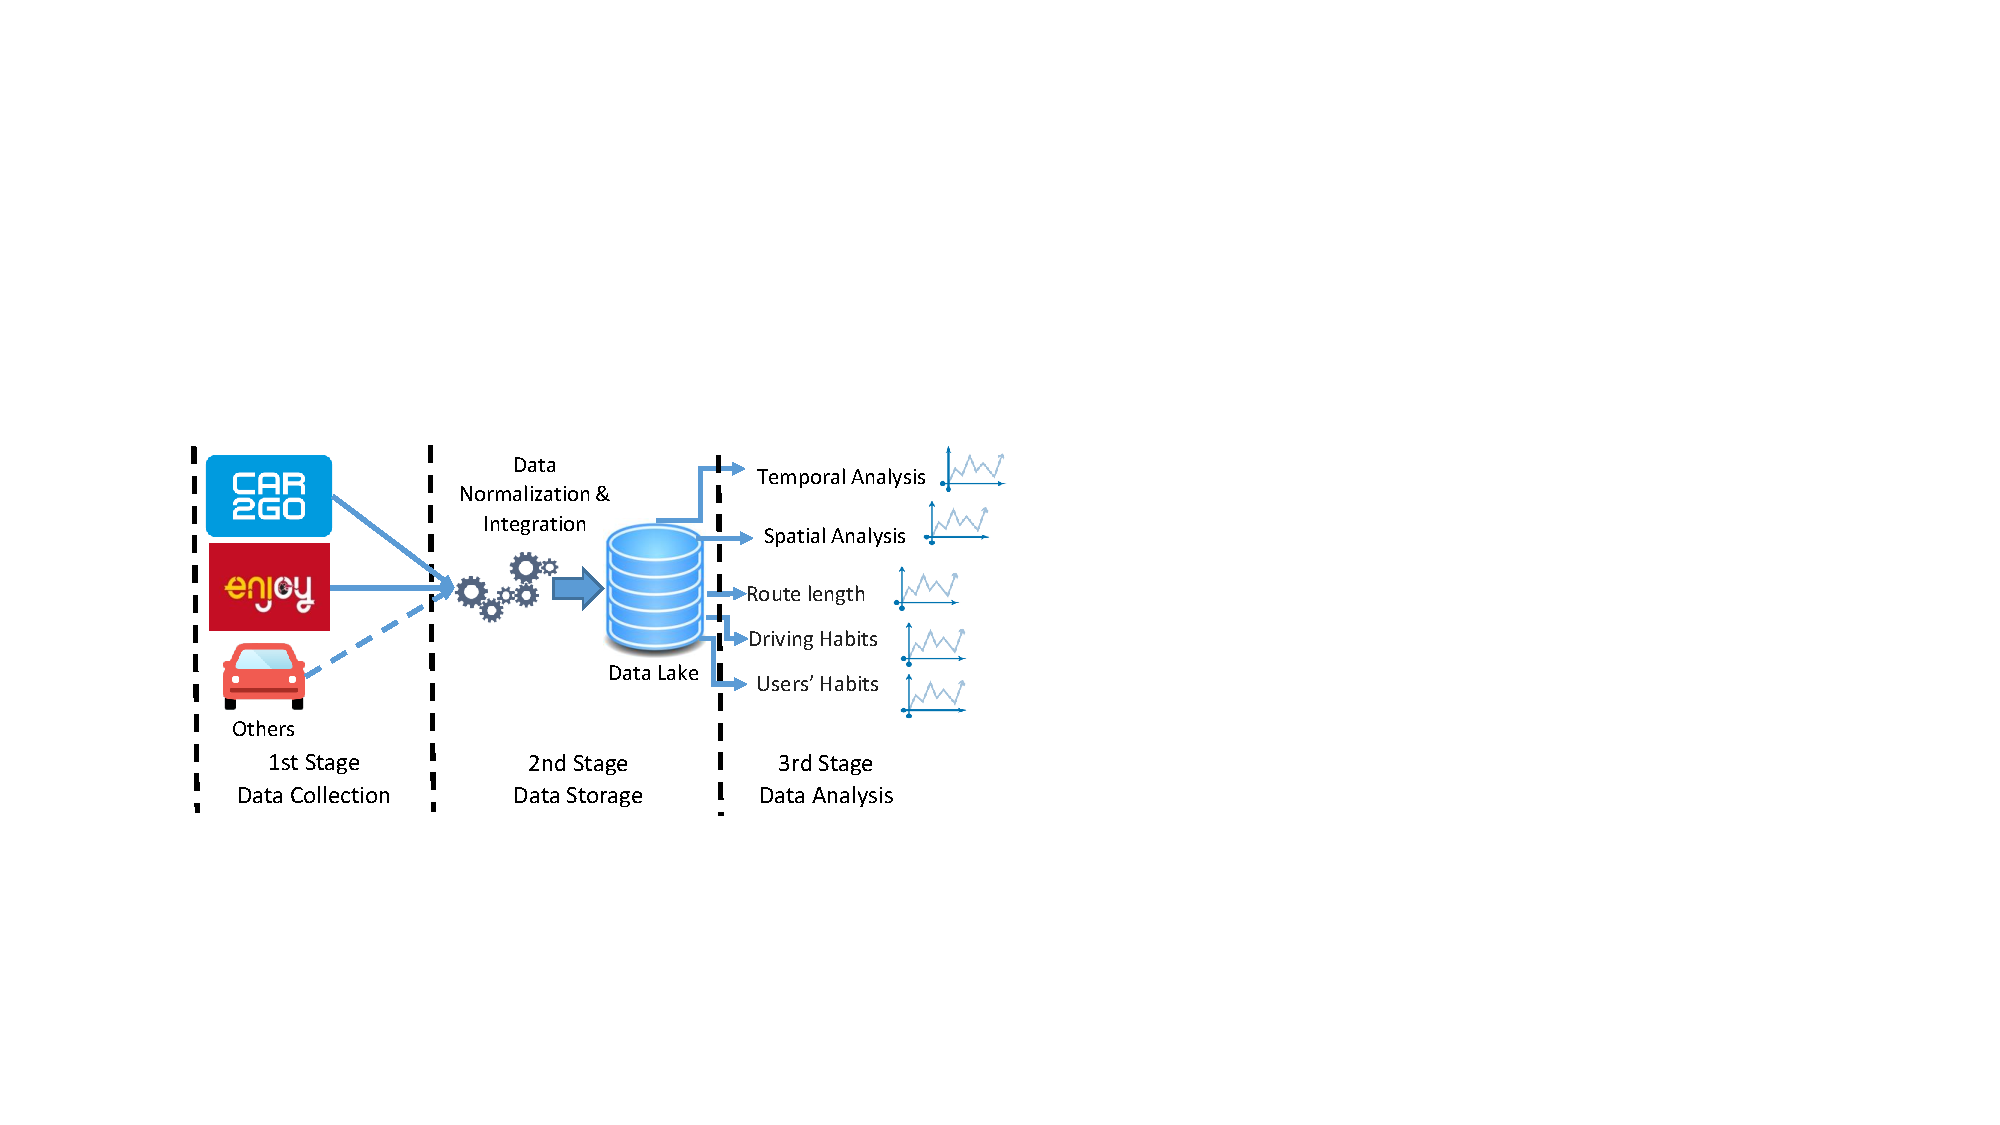
\includegraphics[trim=3cm 4.5cm 17cm 7.2cm,clip, width=0.95\columnwidth]{figures/framework_schema.pdf}
 \caption{\tool overview\label{fig:2_3_c2_framework}}
\end{figure}


In this section, I provide a description of \tool structure. Figure~\ref{fig:2_3_c2_framework} depicts the architecture of \tool, composed by a first module for the data acquisition, by a second module for data normalization and integration, and then a third  module for the data analysis.

The first module consists in the data acquisition from the car sharing platforms of interest. These typically expose information about cars' location when available for rental through a web-service approach. 

For this module I design two crawlers, one for the car2go and one for the Enjoy car sharing platforms. They retrieve, at each time instant, which cars are available in a given city.

While car2go offers public APIs~\cite{car2goAPI}, Enjoy does not provide to users such a service. For this reason I reverse engineer the Enjoy web portal. By leveraging the Chrome Developer Tools, I investigate the information exchanged with the Enjoy web portal while asking the list of available cars. Through this analysis, the software obtains both the URL used to request the list of available cars, and how fetch the data for a specific city.
Both system return the currently available cars using a JSON file.

Each time the system downloads a JSON, a \textit{snapshot} describing which cars are parked and ready for rental. Basically, the \textit{snapshot} is a list containing all cars and their attributes.

In a nutshell, a car is described by the car sharing web-service as an object annotated by several information, like plate, vehicle identification number (VIN), location, fuel level, model, etc. 
All the data represented in this object is useful for the customers e.g., to choose which car to rent.
This object is only present if the car is available, i.e., it is parked and free for a rental. Its state changes over time. In particular, a car disappears when a customer reserves and rents it, and then it reappears when the customer ends the rental (likely in a different location).


At each time $t$, the software gets the JSON snapshot $S$ listing the available cars. 
%We take a snapshot \textit{$S$} every minute to balance aggressiveness of the crawler, and time resolution. 
%At each time t, we obtain from each platform the JSON snapshot S detailing the available cars. 
The sampling period has been set to one minute, to balance aggressiveness of the crawler and a reasonable time resolution.
$S$ describes each available car with several fields, some of them being in common between the considered companies, but in general with different format.
For this study, I collect each car unique identifier and current geo-location indication.
These are obtained from the \textit{VIN} or \textit{plate} field, and the \textit{coordinates} field which describes the \textit{longitude} and the \textit{latitude} of the in-car GPS used to localize it when  parked.\footnote{The GPS coordinates are only available if a car is parked and available. There is no risk for users' privacy during rentals. In addition no user's identifier is exposed. Therefore data is totally anonymized as there is no means to know who booked a car.}
In addition to these fields, the car sharing JSON description may provide other information, e.g., the \textit{street address} corresponding to the coordinates, the \textit{fuel} level, the \textit{car interior status} the \textit{engine type}, etc. Since each platform uses its own data and format, I design a data integration step to have common names for fields containing the same information, if present.

\section{Data Normalization and Integration}
\label{sec:2_4_data_normalization}
In this second module I illustrates hoe \tool processes and consolidate each snapshot to obtain \emph{parking} and \emph{bookings} periods for each car. A \emph{parking} is time where the car is available for a user ride. On the other hand a \emph{bookings} is time elapsing two parking where the car is not tracked by the system. The intuition is to track the availability of each car on the car sharing platform, and rebuild the historic parking and booking periods over time: when a customer books a car, the latter ``disappears'' from the system. The framework records this event, with the initial time and position of a new booking. When the customer ends the booking, the car ``reappears'' in the system. The software records this event, with the final time and position of the booking. For the same car, a new parking period starts.

Harvested data is unstructured, and may grow large. Thus I leverage on \textit{MongoDB}, a NoSQL document-based database. A MongoDB database includes a set collections, i.e., groups of documents. Each document is a set of key-value pairs, organized in a JSON structure. The schema-less structure of MongoDB fits well in this work, because it can handle in the same collection documents defined with different key-value pairs. I decide to rely on such a system as I can easily manage the different field structures of providers, car2go and Enjoy in this use case. In addition, MongoDB offers a great integration with Python through the \textit{pymongo} module.

Four different collections compose the MongoDB data lake:  \textit{ActiveBookings}, \textit{ActiveParkings}, \textit{PermanentBookings}, and \textit{PermanentParkings}. 
\textit{ActiveBookings} and \textit{ActiveParkings} are collections used to store information about the current status of cars (currently booked or parked respectively). These are temporary structures that make it easier to query each car last observed status, and update it. These are also instrumentals for a real-time analysis of the system, e.g., to count how many cars are currently booked or available.
\textit{PermanentBookings} and \textit{PermanentParkings} collections store the history of past state of cars, for past bookings and parkings, respectively.

For the documents in the bookings collections I augment information by inserting also the expected route driving time, and the public transportation duration on the same origin-destination pair. These two piece of information are obtained through the Google Directions API using the initial and the final coordinates as indication of the path.

The most important fields in the \textit{ActiveBookings}, and the \textit{PermanentBookings} collections are:
\begin{itemize}
\setlength\itemsep{0.1em}
\item \textit{CarID}: the unique identifier of the car;
\item \textit{InitTime}: the initial time of the booking;
\item \textit{FinalTime}:  the final time of the booking;
\item \textit{InitCoords}:  the GPS coordinates of the booking star location, i.e., where the users picked up the car;
\item \textit{FinalCoords}:  the GPS coordinates of the parking location where the car was dropped at the end of the booking;
\item \textit{DrivingTime}: The duration of the trip, expressed in seconds, as estimated by Google Directions API, following the best path;
\item \textit{PublicTransportTime}: The duration is expressed as arrival time of the best public transport trip, as estimated by Google Directions API, minus the \textit{InitTime};
\end{itemize}

Instead, the \textit{ActiveParkings} and the \textit{PermanentParkings} collections are characterized by the following fields:
\begin{itemize}
\setlength\itemsep{0.1em}
\item \textit{CarID}: the unique identifier of the car
\item \textit{InitTime}: the initial time of the parking
\item \textit{FinalTime}:  the final time of the parking
\item \textit{Coordinates}: the GPS coordinates of the parking spot 
\end{itemize}

\begin{figure}[t!]
 \removelatexerror
 \scriptsize
  \begin{algorithm}[H]
   	\caption{Data acquisition at time $t$}
	\SetKwInOut{Input}{Input}\SetKwInOut{Output}{Output}
	\Input{$t$ - Current timestamp}
	\Input{$S$ - Available Cars (crawling result)}
	\BlankLine

	$AP$ = $Read(ActiveParkings)$ // Get previous available cars
	
	%\tcc{disappearedCars is a temporary list used to check the cars that %were visible, and that disappeared in the current crawling. In the %beginning the set will be equal to all the active Parkings}
	%$disappearedCars$ = $activeParkings$ \;
	\For(){$car_j$ in $S$}
	{
		\If{($car_j$  in $AP$)}
		{
			%\tcc{Update the parking information for that car with the %current timestamp}
			%$histogramNeighbours[final_time]$ = $current_timestamp$\;
			del $AP[car_j]$\;
		}
		\Else
		{
			$ActiveParkings.add(new~Parking(car_j,t))$\;		
			\If{($car_j$  in $ActiveBookings$)}
			{
				$FinalCoords = car_j[coords];$
				
				$ActiveBooking[car_j][FinalTime] = t$\;
				
				$InitCoords = ActiveBookings[car_j][InitCoords];$	
						
				\If{(checkCarMovement($InitCoords$,$FinalCoords$))}
				{
					$ActiveBooking[car_j][driving\_time]$ = $GoogleApi(driving,InitCoords,FinalCoords)$\;
					$ActiveBooking[car_j][PublicTranportTime]$ = $GoogleApi(public,InitCoords,FinalCoords)$\;
				}
				$MoveRow(car_j,ActiveBooking,PermanentBooking)$;
			}
			}
	}
	\For(){$car_j$ in $AP$}
	{
		$ActiveParking[car_j][FinalTime] = t$\;
		$MoveRow(car_j,ActiveParking,PermanentParking)$\;
		$ActiveBooking.add(new~Booking(car_j,t))$\;		
	}
  \end{algorithm}
   \caption{Pseudocode of the data acquisition algorithm}\label{pseudocodeCarInfoUpdate}
\end{figure}




I implemented an algorithm to extract booking and parking periods from snapshots, whose workflow is described in the pseudocode in Figure.~\ref{fig:3_2_c2_pseudocodeCarInfoUpdate}. Here I describe each  step.

I consider as inputs the snapshot $S$ and the current timestamp $t$.
Then I create a copy in the list $AP$ of parked cars observed in the previous snapshot (as stored in the $ActiveParkings$ collection) -- line 1. I need the $AP$ list to detect the cars that disappeared, i.e., have been booked at time $t$. This will be back explained later.

For each car $car_j$ in the current snapshot $S$, I check if the car is present in the $AP$ list. 
If so, it means that it did not change its status, i.e., it is still parked. Therefore, the car is removed from the $AP$ list, and nothing is changed -- lines 3-4.
Otherwise, either the car has been parked in this snapshot and the previous booking has finished, or the car is a new car added to the fleet. In both cases a new parking starts and I create a new document in the $ActiveParkings$ collection -- line 7. The \textit{new Parkings} function creates a new document, sets the $InitTime$ and $Coordinates$ keys as current timestamp and car GPS coordinates.
%with the current timestamp and the car GPS coordinates.

I next check if $car_j$ is present in the $ActiveBookings$ collection. If so, the car was booked until the previous snapshot and now it is back available. I thus finalize the previous booking and update its statistics. In particular, the tool sets the $FinalCoords$ and $FinalTime$ fields using the current car $coordinates$ and timestamp -- line 9-10. Next, I check if this booking includes an actual rental by checking if the initial position and final position differ -- line 11-12. Recall indeed that customers may simply book a car but not finalize the rental. Specifically, Enjoy (car2go) offers a grace period of 15 (20) minutes during which no charge is applied for a booking.

In case of an actual rental, I fetch the best path by i) car and ii) public transport from the  $InitPosition$ to the $FinalPosition$ of the rental. I leverage the Google Directions API for this -- line 13-14.\footnote{\url{https://enterprise.google.com/intl/it/maps/products/mapsapi.html}}
It is important to take into account that, while querying the public transportation time, the Google Directions API returns two pieces of information: how long the public transport takes to go from the initial to the final position, and the estimated arrival time. It is fundamental to use this second information because  it includes the time the user spends to reach the bus stop and wait for the bus. This is crucial, e.g., at night, when the first public transport solution may be available only several hours later.

After having processed all cars in the current snapshot, I iterate over the remaining cars in the $AP$ list. Those are the ones that were present in the previous snapshot, but not in the current, i.e., the ones the new bookings. Finally, the software adds to the previous parking period by setting the $FinalTime$ in the $ActiveParking$ collection -- line 21-22. At last, the tool creates a new booking via the \textit{new Booking} function -- line 23.


\begin{table}
	\setlength{\tabcolsep}{2.3pt}
	\centering
	\caption{Overview of car2go's data}
	\begin{tabular}{lcccc}
		\hline
		City &  City Size [$km^2$]\footnote{} & Population \footnotemark[\value{footnote}] &  Avg. Fleat & Bookings\\ 
		\hline
		\hline
		Columbus			  & 17 & 892k & 187 & 186k \\
		Florence 	  			& 34 & 372k & 220 & 333k \\
		Denver 		  			 & 36 & 727k & 312 & 348k \\
		Austin 		   			  & 31 & 964k & 315 & 377k \\
		Frankfurt 			   & 40 & 701k & 242 & 505k \\
		Toronto 				 & 49 & 3120k & 400 & 536k \\
		Amsterdam 			& 38 & 854k & 314 & 573k \\
		Montreal 				& 49 & 1704k & 429 & 606k \\
		New York City 	   & 77 & 8522k & 500 & 739k \\
		Turin 					    & 47 & 874k & 396 & 868k \\
		Munich 					 & 61 & 1464k & 478 & 916k \\
		Washington DC 	  & 64 & 705k & 563 & 919k \\
		Stuttgart 				 & 59 & 632k & 486 & 1001k \\
		Seattle 				   & 92 & 744k & 710 & 1134k \\
		Calgary 				  & 47 & 1239k & 552 & 1176k \\
		Rome 					  & 65 & 2837k & 582 & 1240k \\
		Rheinland 			   & 82 & 1688k & 648 & 1421k \\
		Vienna 					  & 72 & 1915k & 688 & 1702k \\
		Madrid 					 & 42 & 3233k & 424 & 2092k \\
		Milan 					   & 77 & 1396k & 776 & 2223k \\
		Hamburg 			  & 82 & 1833k & 812 & 2561k \\
		Vancouver 			 & 78 & 631k & 977 & 2701k \\
		Berlin 					  & 125 & 3769k & 1009 & 3091k \\
		%\\ \hline
		\hline
		\label{tab:2_3_datasummary}
	\end{tabular}
\end{table}
\footnotetext{\url{wikipedia.org}}
I let \tool scrape car2go's data  \mc{prendere le date}. In total it is possible to count about 27 million bookings spread in 23 cities. The table \ref{tab:2_3_datasummary} reports a brief resume of all the bookings, parkings present in the data lake. 

\mc{devo prendere le date anche di enjoy}



\section{Data Analysis}
The third and final stage is the data analysis phase in which analytics modules query the MongoDB and obtain statistics. I rely on the Python programming language with Pandas and the GeoPandas libraries to deal with the data, the city zone definitions, provided by transport engineers as a shapefile, a popular geospatial vector data format, and the Geographical Information Systems (GIS) for the spatial analyses. I choose Python as it offer a large number of  libraries that easily interact with the different technologies like GIS, maps and MongoDB. In particular the usage of GeoPandas allow me to easily perform geographic analysis and split the city in many areas (or zones) of any possible shapes. I present more detailed characterization in chapter \ref{chap:3_charact}.


\section{Conclusion}
In this chapter I described the software pipeline, named \tool I used to harvest and store data from real FFCS providers. 

The first stage explains the data structures and how I snapshots the system getting all the car ready for a ride. 

The seconds step illustrates the algorithm that compares consecutive snapshots detecting car status variation. Here I introduced the two fundamental car status I use to describe each car history: \textit{parkings} and \textit{bookings}. 

The third briefly opens several scenarios on the analyses of this data.



% !TEX root = ../toptesi-scudo-example.tex
% !TEX encoding = UTF-8 Unicode
%***********************************************************************
%***********************************Second Chapter
%***********************************************************************

\chapter{Dataset Characterization}
\label{chap:3_charact}
	\graphicspath{{Chapter3/}}

\section{Abstract}
\section{Abstract}
\label{sec:3_0_abstract}

The understanding of the mobility on urban spaces is useful for the creation of smarter and sustainable cities. However, getting data about urban mobility is challenging, since only a few companies have access to accurate and updated data, that is also privacy-sensitive. 

In this work, we characterize three distinct car-sharing systems which operate in Vancouver (Canada) and nearby regions, gathering data for more than one year. Our study uncovers patterns of users' habits and demands for these services. 
We highlight the common characteristics and the main differences among car-sharing systems. Finally, we believe our study and data is useful for generating realistic synthetic workloads.

\section{Introduction}
\label{sec:3_1_intro}

Mobility is one of the challenges to solve in our society and in cities, where eco-sustainability is becoming more and more important. 
Regulators and policy makers are positively looking into ``smart'' approaches to improve the current status of their urban network.  The ability to inspect data, is the first step to take informed decisions. Unfortunately, getting information about mobility patterns and human driving habits is not easy because of both technical challenges and privacy issues.

Car sharing refers to a model of car rental where customers rent a car for a short period of time, usually for a few hours or less. One of its most interesting systems is the so called \textit{Free-Floating Car Sharing (FFCS)} system. The peculiarity of this system is that customers can pick and drop the car wherever in a geo-fence area.
The most famous company is car2go which is present in 25 cities and 8 different countries, both in Europe and North America \footnote{The service is discontinued in North America since February, $29^{th}$ 2020, \url{https://www.share-now.com/ca/en/important-update/}}.

To rent a car in a modern FFCS system, users check on their smartphone, or on the FFCS website, which cars are available in the neighborhood. Then, with a simple tap they can book a car, and start/end the rental. The FFCS app contacts a web-based back-end server to fetch data about available cars, perform a booking, and accounting operations. Typically for this purpose web API are used, some of which are publicly documented~\cite{car2goAPI}. The same website and app offer information about the status of the car rental systems, and the same web API can be used to collect for free this information. In the past, this approach has been successfully used to obtain data for specific mobility studies -- see Sec.~\ref{sec:3_2_related} for more details. 
This chapter relies on the tool described in chapter \ref{chap:2_dataset}. In particular, I analyze the first chunk of data I was able to collect. I let the crawlers run for 52 days,  from December 10th 2016 to January 31st 2017. In total \tool collected more than 104,000 \textit{bookings} for car2go and 93,000 \textit{bookings} and for Enjoy. 

%and 86,000 \textit{rentals}
%81,000 \textit{rentals}

With these datasets, after a first cleaning phase where I detected entries corresponding to trips where the users actually made a ride, I characterize the FFCS service utilization with the aim to observe how people use these services, where they typically go, when, for how long the rental last, etc. Some observations are quite intuitive, e.g., people appear to be willing to use more the FFCS during weekdays and during peak-time. Counterintuitively, the rental duration and the driving distance show marginal changes over the day and weeks.

I complement the analysis by comparing the ride duration with the driving duration as suggested by Google Directions application, which the software can collect in real time for each rental. This highlights that 8.5\% of bookings last less than the Google driving time. 
This may be due to Google Directions overestimating the driving duration or, recalling that bookings  include the reservation time and the time to look for a parking spot, this may suggest that the time-based tariffs adopted by FFCS systems may encourage fast driving styles in the hope to reduce the rental cost.
I next compare the duration of the booking with the equivalent trip duration by public transport as returned again by Google Directions. I discover that rentals are 36\% shorter on average than public transport time, but  rentals start to be preferred when public transport time is higher than 10 minutes.

\tool may represents an important support tool for the investigation of car sharing users' habits. The scalable design of \tool allows the policy maker to collect data from many FFCS providers  and integrate it with other sources. This eases the analysis when taking in consideration trends and providers comparison. \tool allows the Transportation Authority to take informed decisions when planning public transport systems. This characteristic strengthens the potentiality of \tool for economical and sociological prediction and analysis. The data-driven approach, combined with other more traditional tools like surveys, represents an interesting observation point for understanding potential services improvements, both for car sharing and public transport systems. The source code of \tool  is available for research purposes.\footnote{\url{github.com/MobilityPolito/}}

The reminder of this chapter is structured as follows: Sec.~\ref{sec:3_2_related} discusses the related works. Sec.~\ref{sec:3_4_results} presents the in the following order: First, car2go and Enjoy car usage over time characterization; second, how customers drive the cars and how they move in the city; finally, users' driving habits and the correlation between booking time and the public transport time. Sec.~\ref{sec:3_5_conclu} concludes the chapter.
\mc{da rivedere}



\section{Related Work}
\label{sec:3_2_related}
%Since Free Floating approach for car sharing (FCSS) started to propagate, many researchers from different fields analyzed this topic. 
Since the diffusion of the new form of car sharing based on a free-floating approach, many researchers from different fields have been dedicating an increasing attention to the analysis of these systems.
The high demand for car sharing has opened new challenges and perspectives in research.

One of the main topics is the study of fleet relocation policies~\cite{Herrmann2014,Schulte2015,Wagner2015}. On the one hand, with respect to station-based car sharing, the flexibility of the free-floating system may limit the operator's control over the drop-off zones, but on the other hand allows smarter strategies. 
%Herrmann1024 -> car2go api into simulation environment
Herrmann, Schulte and Voß~\cite{Herrmann2014} conducted a survey to understand how the availability of cars, and so the fleet relocation, affects the utilization of the service, and to develop and evaluate user-oriented relocation strategies.
%Schulte2015 -> api car2go
Those strategies were studied again by Schulte and Voß~\cite{Schulte2015}, who introduced an approach to support the decision of vehicle relocation method to reduce costs and emissions in FFCS.
%Wagner2015 -> As one of the main contributions of this paper, we conduct an extensive case study for the city of Berlin in cooperation with a globally leading car sharing provider. Rental data of 1,200 shared vehicles was collected over a period of 1 year.
Those kind of investigations may result in a very useful support for the providers. In this direction, Wagner, Brandt and Neumann \cite{Wagner2015}, analyzed the use of car sharing in Berlin, using indicators of actractiveness of certain areas, in order to develop a methodology that is able to help in business strategies, the expansion of operative areas and to react to shifts in demand. In these works, the authors used data collected from car sharing providers, using the car2go API~\cite{Herrmann2014,Schulte2015} or by a direct cooperation \cite{Wagner2015}.

%Schmoller2015 -> The first data set obtained by the operator contains the current number of vehicles and registered members for both cities for each day of the investigation period. The second and most important data set contains the booking data of the operator for a period of two years, from November 1, 2011 to October 31, 2013
The study of the customers' behavior has been addressed by different researchers~\cite{Schmoller2015,Kopp2015,Firnkorn2012,Ciari2013,Tyndall2016}. 
Schmöller et al.~\cite{Schmoller2015} studied factors that may influence the demand of car sharing, carrying out an empirical analysis, considering FFCS in Berlin and Munich.
%Kopp2015 To collect the mobility behaviour, an active tracking approach was chosen for MyMobility
Kopp et al.~\cite{Kopp2015} inspected the behavior of two categories of users, the members of a FFCS service (DriveNow), and the people who do not use car sharing (NCS users), looking for different and distinctive mobility patterns.
%Firnkorn2012 invitation emails with links to the survey
The impact of car sharing on people's mobility was addressed by Firnkorn~\cite{Firnkorn2012}, who proposed in its work a triangulation of two methods applied in the same survey, to provide more precise measurements.
%Ciari2013
Another approach was proposed by Ciari et al.~\cite{Ciari2013}, where a simulation tool, built on MATsim, an open source project, was used to estimate travel demand for car sharing in the urban area of Zurich.
An important question that can be addressed is how this new paradigm of transport is really accessible to the people. Tyndall \cite{Tyndall2016} combined data of FFCS usage in ten US cites with demographic information, studying neighbourhood infrastructures, population distribution and their mobility habits. It has been showed that  benefits of FFCS are distributed unequally, with a shift on usage in favor of advantaged populations.

%Firnkorn2011 Based on primary data from a survey
Eco-sustainability is another important asset for car sharing services. Firnkorn and Müller~\cite{Firnkorn2011} studied the environmental effects of FFCS in Ulm, registering lower pollution levels and a reduction of private vehicle ownership.

The goal of our work is to address all these challenges from the local administration's perspective, in order to develop new transport and mobility policies.
A study of this kind was recently conducted by Wang et al. \cite{Wang2017} for the city of Seattle, where car2go was compared with public transport service.
Kortum et al. \cite{Kortum2016} remark the necessity of use data-driven approaches to help decision making, due to the lack of empirical data about free-floating car sharing usage. 
They use a dataset, obtained by InnoZ (Innovationszentrum für Mobilität und gesellschaftlichen Wandel) and containing the activity in 33 cities from 2011 to November 2015, to study the evolution in time of this mobility service. Those data, combined to demographic informations, offered an aggregated point of view, over different cities, of the growth of the car sharing service and an understanding of the main characteristics.
To the best of our knowledge, in the context of our case of study, the only work on free-floating car sharing was conducted by Ferrero et al. \cite{Ferrero2016} from an economical point of view.

The majority of the previous works \cite{Herrmann2014,Schulte2015,Wagner2015,Schmoller2015,Kopp2015,Wang2017,Kortum2016} leverage data collected in real-time or using surveys and interviews. Thanks to car2go APIs, which easily make avaiable car sharing data, a more data-driven approach is attractive for many researchers that start facing the problem of FFCS mobility analysis. Remarkably, only \cite{Kortum2016} seems to use data collected actively by different car sharing providers. While authors use information only for a specific purpose i.e., analyzing the trend of car sharing through the years, here we want to provide a broader perspective.
Our intent is indeed to offer a general purpose methodology, both scalable and easy to interact with, to help researchers and local administrations in the analysis of the mobility, harvesting data collected from FFCS platforms, but also from other online systems, like mapping and direction services. 
%We offer an engaging platform, with the couple of both pre-computed analysis and tools to develop new ones, on different operators over the city of Turin. 


%\section{Methodology}
\label{sec:methodology}


\begin{figure}[h!]
\centering
%left top right top
 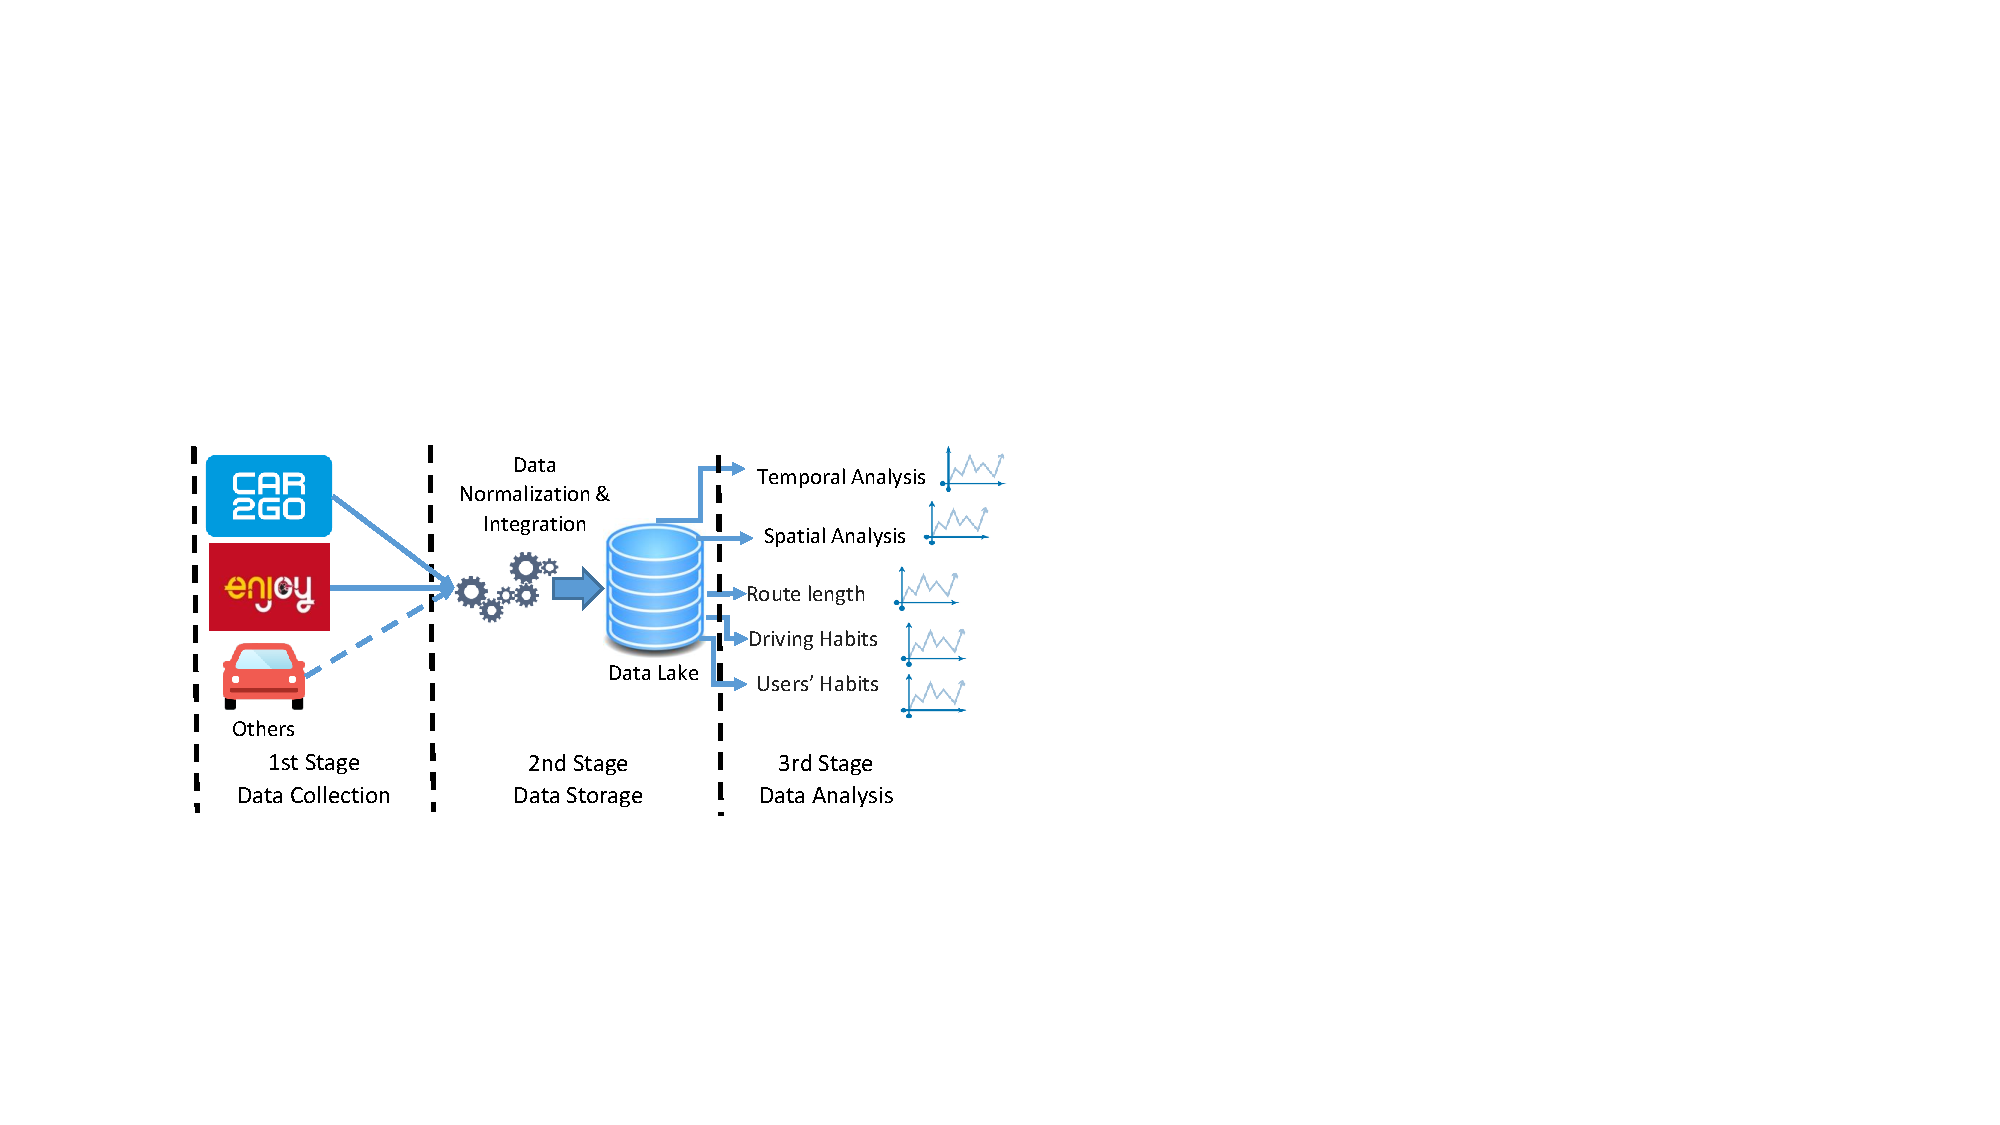
\includegraphics[trim=3cm 4.5cm 17cm 7.2cm,clip, width=0.95\columnwidth]{figures/framework_schema.pdf}
 \caption{\tool overview\label{fig:framework}}
\end{figure}



Our goal is to develop \tool, an integrated system to harvest data freely made available on the web and related to driving habits in cities. \tool offers processing capabilities to perform several analysis and extracting useful information about driving and users' behavior.


In this section, we provide a description of \tool. Figure~\ref{fig:framework} depicts the architecture of \tool, composed by a first module for the data acquisition, by a second module for data normalization and integration, and then a third  module for the data analysis.


\subsection{Data Acquisition}

The first module consists in the data acquisition from the car sharing platforms of interest. These typically expose information about cars' location when available for rental through a web-service approach. 

For this module we design two crawlers, one for the car2go and one for the Enjoy car sharing platforms. They retrieve, at each time instant, which cars are available in a given city.

While car2go offers public APIs~\cite{car2goAPI}, Enjoy does not provide to users such a service. For this reason we study and reverse engineer the Enjoy web portal. By leveraging the Chrome Developer Tools, we investigate the information exchanged with the Enjoy web portal while asking the list of available cars. Through this analysis, we obtain both the URL used to request the list of available cars, and how fetch the data for a specific city.
Both system return the currently available cars using a JSON file.

Each time we download a JSON, we discover a new \textit{snapshot} describing which cars are parked and ready for rental.

In a nutshell, a car is described by the car sharing web-service as an object annotated by several information, like plate or vehicle identification number (VIN), location, fuel level, model, etc. 
All the data represented in this object is useful for the customers e.g., to choose which car to rent.
This object is only present if the car is available, i.e., it is parked and free for a rental. Its state changes over time. In particular, a car disappears when a customer reserves and rents it, and then it reappears when the customer ends the rental (likely in a different location).


At each time $t$, we obtain the JSON snapshot $S$ listing the available cars. 
%We take a snapshot \textit{$S$} every minute to balance aggressiveness of the crawler, and time resolution. 
%At each time t, we obtain from each platform the JSON snapshot S detailing the available cars. 
The sampling period has been set to one minute, to balance aggressiveness of the crawler and a reasonable time resolution.
$S$ describes each available car with several fields, some of them being in common between the considered companies, but in general with different format.
For this study, we are interested in each car unique identifier and current geo-location indication.
These are obtained from the \textit{VIN} or \textit{plate} field, and the \textit{coordinates} field which describes the \textit{longitude} and the \textit{latitude} of the in-car GPS used to localize it when  parked.\footnote{The GPS coordinates are only available if a car is parked and available. There is no risk for users' privacy during rentals. In addition no user's identifier is exposed. Therefore data is totally anonymized as there is no means to know who booked a car.}
In addition to these fields, the car sharing JSON description may provide other information, e.g., the \textit{street address} corresponding to the coordinates, the \textit{fuel} level, the \textit{car interior status} the \textit{engine type}, etc. Since each platform uses its own data and format, we design a data integration step to have common names for fields containing the same information, if present.

\subsection{Data Normalization and Integration}

In this second module we process and consolidate each snapshot to obtain rentals and parking periods for each car. The intuition is to track the availability of each car on the car sharing platform, and rebuild the historic parking and booking periods over time: when some customer books a car, the latter ``disappears'' from the system. We record this event, with the initial time and position of a new booking. When the customer ends the booking, the car ``reappears'' in the system. We record this event, with the final time and position of the booking. For the same car, a new parking period starts.

Harvested data is unstructured, and may grow large. Thus we leverage on \textit{MongoDB}, a NoSQL document-based database. A MongoDB database includes a set collections, i.e., groups of documents. Each document is a set of key-value pairs, organized in a JSON structure. The schema-less structure of MongoDB fits well in our work, because it can handle in the same collection documents defined with different key-value pairs. We decide to rely on such a system as we can easily manage the different field structures of providers, car2go and Enjoy in our use case. In addition, MongoDB offers a great integration with Python through the \textit{pymongo} module.

Four different collections compose our MongoDB data lake:  \textit{ActiveBookings}, \textit{ActiveParkings}, \textit{PermanentBookings}, and \textit{PermanentParkings}. 
\textit{ActiveBookings} and \textit{ActiveParkings} are collections used to store information about the current status of cars (currently booked or parked respectively). These are temporary structures that make it easier to query each car last observed status, and update it. These are also instrumentals for a real-time analysis of the system, e.g., to count how many cars are currently booked or available.
\textit{PermanentBookings} and \textit{PermanentParkings} collections store the history of past state of cars, for past bookings and parkings, respectively.

For the documents in the bookings collections we augment information by inserting also the expected route driving time, and the public transportation duration on the same origin-destination pair. These two piece of information are obtained through the Google Directions API using the initial and the final coordinates as indication of the path.

The most important fields in the \textit{ActiveBookings}, and the \textit{PermanentBookings} collections are:
\begin{itemize}
\setlength\itemsep{0.1em}
\item \textit{CarID}: the unique identifier of the car;
\item \textit{InitTime}: the initial time of the booking;
\item \textit{FinalTime}:  the final time of the booking;
\item \textit{InitCoords}:  the GPS coordinates of the booking star location, i.e., where the users picked up the car;
\item \textit{FinalCoords}:  the GPS coordinates of the parking location where the car was dropped at the end of the booking;
\item \textit{DrivingTime}: The duration of the trip, expressed in seconds, as estimated by Google Directions API, following the best path;
\item \textit{PublicTransportTime}: The duration is expressed as arrival time of the best public transport trip, as estimated by Google Directions API, minus the \textit{InitTime};
\end{itemize}

Instead, the \textit{ActiveParkings} and the \textit{PermanentParkings} collections are characterized by the following fields:
\begin{itemize}
\setlength\itemsep{0.1em}
\item \textit{CarID}: the unique identifier of the car
\item \textit{InitTime}: the initial time of the parking
\item \textit{FinalTime}:  the final time of the parking
\item \textit{Coordinates}: the GPS coordinates of the parking spot 
\end{itemize}

\begin{figure}[t!]
 \removelatexerror
 \scriptsize
  \begin{algorithm}[H]
   	\caption{Data acquisition at time $t$}
	\SetKwInOut{Input}{Input}\SetKwInOut{Output}{Output}
	\Input{$t$ - Current timestamp}
	\Input{$S$ - Available Cars (crawling result)}
	\BlankLine

	$AP$ = $Read(ActiveParkings)$ // Get previous available cars
	
	%\tcc{disappearedCars is a temporary list used to check the cars that %were visible, and that disappeared in the current crawling. In the %beginning the set will be equal to all the active Parkings}
	%$disappearedCars$ = $activeParkings$ \;
	\For(){$car_j$ in $S$}
	{
		\If{($car_j$  in $AP$)}
		{
			%\tcc{Update the parking information for that car with the %current timestamp}
			%$histogramNeighbours[final_time]$ = $current_timestamp$\;
			del $AP[car_j]$\;
		}
		\Else
		{
			$ActiveParkings.add(new~Parking(car_j,t))$\;		
			\If{($car_j$  in $ActiveBookings$)}
			{
				$FinalCoords = car_j[coords];$
				
				$ActiveBooking[car_j][FinalTime] = t$\;
				
				$InitCoords = ActiveBookings[car_j][InitCoords];$	
						
				\If{(checkCarMovement($InitCoords$,$FinalCoords$))}
				{
					$ActiveBooking[car_j][driving\_time]$ = $GoogleApi(driving,InitCoords,FinalCoords)$\;
					$ActiveBooking[car_j][PublicTranportTime]$ = $GoogleApi(public,InitCoords,FinalCoords)$\;
				}
				$MoveRow(car_j,ActiveBooking,PermanentBooking)$;
			}
			}
	}
	\For(){$car_j$ in $AP$}
	{
		$ActiveParking[car_j][FinalTime] = t$\;
		$MoveRow(car_j,ActiveParking,PermanentParking)$\;
		$ActiveBooking.add(new~Booking(car_j,t))$\;		
	}
  \end{algorithm}
   \caption{Pseudocode of the data acquisition algorithm}\label{pseudocodeCarInfoUpdate}
\end{figure}




We implemented an algorithm to extract booking and parking periods from snapshots, whose workflow is described in the pseudocode in Fig.~\ref{pseudocodeCarInfoUpdate}. Here we describe each  step.

We consider as inputs the snapshot $S$ and the current timestamp $t$.
Then we create a copy in the list $AP$ of parked cars observed in the previous snapshot (as stored in the $ActiveParkings$ collection) -- line 1. We need the $AP$ list to detect the cars that disappeared, i.e., have been booked at time $t$. We will be back on this later.

For each car $car_j$ in the current snapshot $S$, we check if the car is present in the $AP$ list. 
If so, it means that it did not change its status, i.e., it is still parked. Therefore, the car is removed from the $AP$ list, and nothing is changed -- lines 3-4.
Otherwise, either the car has been parked in this snapshot and the previous booking has finished, or the car is a new car added to the fleet. In both cases a new parking starts and we create a new document in the $ActiveParkings$ collection -- line 7. The \textit{new Parkings} function creates a new document, sets the $InitTime$ and $Coordinates$ keys as current timestamp and car GPS coordinates.
%with the current timestamp and the car GPS coordinates.

We next check if $car_j$ is present in the $ActiveBookings$ collection. If so, the car was booked until the previous snapshot and now it is back available. We thus finalize the previous booking and update its statistics. In particular, we set the $FinalCoords$ and $FinalTime$ fields using the current car $coordinates$ and timestamp -- line 9-10. Next, we check if this booking includes an actual rental by checking if the initial position and final position differ -- line 11-12. Recall indeed that customers may simply book a car but not finalize the rental. Specifically, Enjoy (car2go) offers a grace period of 15 (20) minutes during which no charge is applied for a booking.

In case of an actual rental, we fetch the best path by i) car and ii) public transport from the  $InitPosition$ to the $FinalPosition$ of the rental. We leverage the  Google Directions API for this -- line 13-14.\footnote{\url{https://enterprise.google.com/intl/it/maps/products/mapsapi.html}}
It is important to take into account that, while querying the public transportation time, the Google Directions API returns two pieces of information: how long the public transport takes to go from the initial to the final position, and the estimated arrival time. It is fundamental to use this second information because  it includes the time the user spends to reach the bus stop and wait for the bus. This is crucial, e.g., at night, when the first public transport solution may be available only several hours later.

After having processed all cars in the current snapshot, we iterate over the remaining cars in the $AP$ list. Those are the ones that were present in the previous snapshot, but not in the current, i.e., the ones the new bookings. We finalize the previous parking period by setting the $FinalTime$ in the $ActiveParking$ collection -- line 21-22. At last, we create a new booking via the \textit{new Booking} function -- line 23.
% Finally, the \textit{add} function add this document to the $ActiveBooking$ collection.}


\subsection{Data Analysis}

The third and final step is the data analysis phase in which analytics modules query the MongoDB and obtain statistics. We rely on the Python programming language with Pandas and the GeoPandas libraries to deal with the data, the city zone definitions,
provided by transport engineers as a shapefile, a popular geospatial vector data format,
 and the Geographical Information Systems (GIS) for the spatial analyis. We choose Python as it offer a large number of  libraries that easily interact with the different technologies like GIS, maps and MongoDB. In particular the usage of GeoPandas allow us to easily perform geographic analysis and split the city in many areas (or zones) of any possible shapes. We describe each analytics in the next section. We present results considering the city of Turin as an example of their usage.



\section{Temporal Analyses}
\label{sec:results}

In this section I show different analysis to discover and characterize how the FFCS are used. In the first part of the section, I analyse the temporal systems characterization to understand if FFCS are actually used and when.

I consider a period from December 10th 2016 to January 31st 2017, the first reliable collected data chunk. The system observed 125,000 snapshots, about 104,000 bookings for car2go and 93,000 for Enjoy. In Turin, the fleet of car2go was composed by 394 cars, and the fleet of Enjoy was composed by 172 cars.

In order to make clear the rest of the book, it necessary to univocally define the basilar entities related to the car status in the data lake defined in the chapter \ref{chap:2_dataset}, section \ref{sec:2_4_data_normalization}.

\begin{definition}{the \textbf{Parking}}
	\label{def:parking} is the time period in which the car is present in, at least, two consecutive snapshot. Therefore that car it is available for an user reservation
\end{definition}
\begin{definition}{the \textbf{Booking}}
	\label{def:booking} is the time period in which the car is NOT present in, at least, two consecutive snapshot. There fore an user booked that vehicle or the provider temporary removed it for maintenance.
\end{definition}


\subsection{System Utilization}

\begin{figure}
\centering
 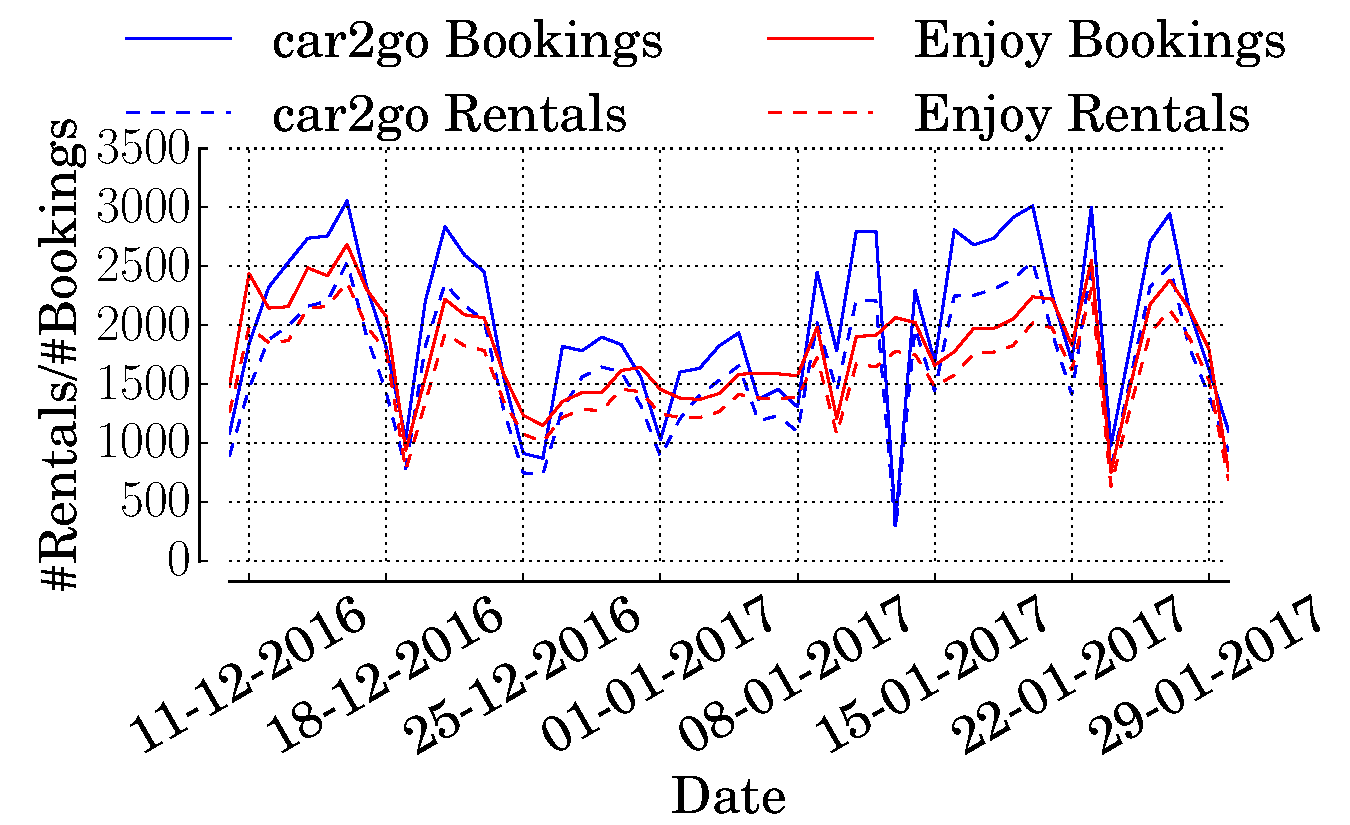
\includegraphics[width=0.85\columnwidth]{figures/bookings.pdf}
 \caption{Total number of bookings and of rentals per day for car2go and for Enjoy \label{fig:bookings}}
\end{figure}
The providers, in this case study, allows the users to \textit{reserve} a car before the ride. More in details, the provider makes the reserved car unavailable for the other users without billing the customer who reserved the car. When the reservation time (that changes for each provider), the billing mechanism starts even if the engine it is still off. The customer can cancel the reservation without any expense if it happens before the reservation time. With this mechanism, the providers would let the possibility to the users to reach the cars by foot.

Given that, it is now possible to the define:
\begin{definition}{\textbf{Reservation}}
	\label{def:reservation} A reservation it is a booking where the initial and final destination matches and the duration is lower than the provider's reservation time.
\end{definition}

\begin{definition}{\textbf{Rental}}
	\label{def:rental} A rental it is a booking where the initial and final destination are different.
\end{definition}


Starting from December 10th, Figure~\ref{fig:bookings} plots the total number of bookings and the total number of rentals recorded on each day, for car2go (blue curves), and for Enjoy (red curves). Obviously, being the latter a subset of the first, its number is always smaller. However, during some days, the discrepancy is well visible; that means that the operation of booking cancellation is not so rare.

Interestingly, firstly, both car2go and Enjoy follow a similar behaviour with the number of bookings and rentals decreasing in the Christmas period and increasing again after the Epiphany. 

Secondly, despite car2go fleet has more than twice as much cars than Enjoy (394 vs. 172), the number of car2go bookings does not show such a higher value with respect to Enjoy. With Enjoy having more bookings in some snapshots e.g., December 10th and 11th. Moreover, in some points (ecember 19th, January 24th) it is possible to detect huge drop due to the failure of our crawler. 

Moreover, some drops in bookings' values are noticeable. Those sudden changes can be addressed to some failures, in the crawlers (e.g., when all curves suddenly drop) or in the operators' web services(e.g., when only one system suffers a sudden drop).



\begin{figure}
\centering
 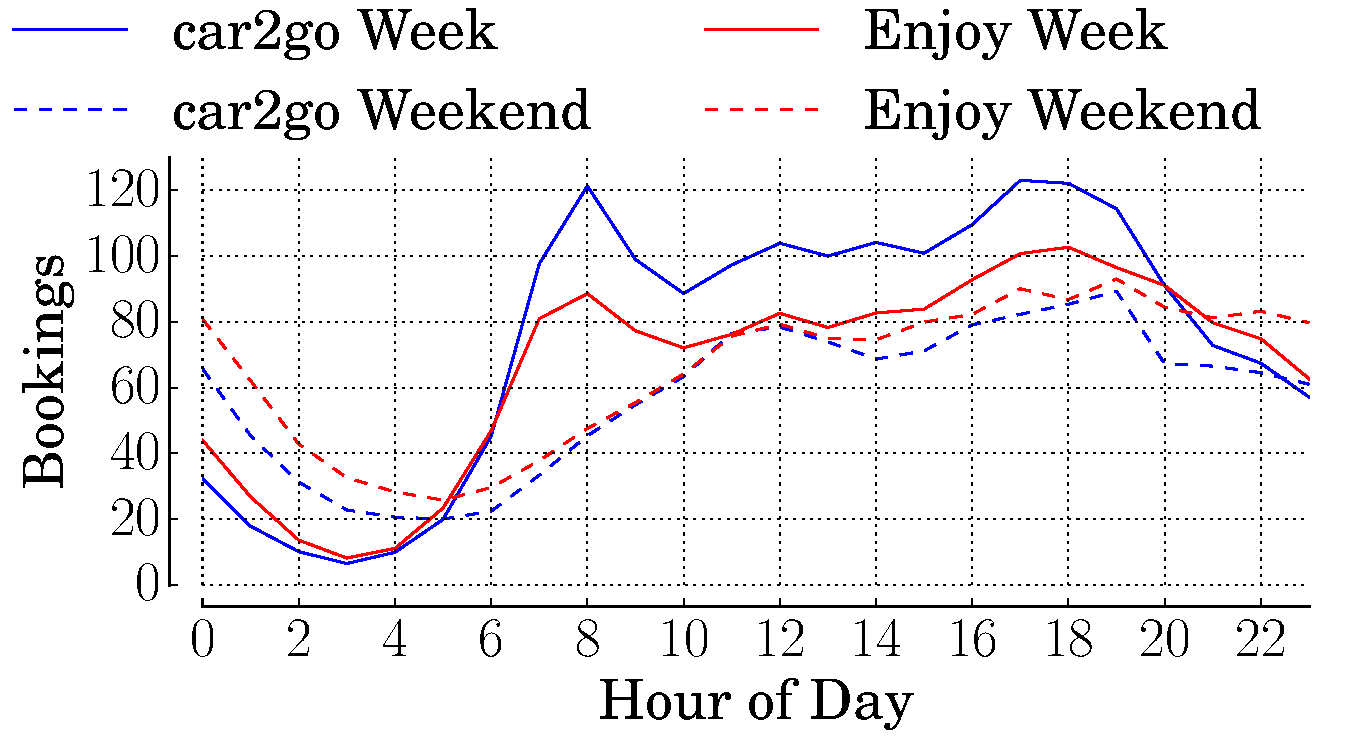
\includegraphics[width=0.85\columnwidth]{figures/bookings_day.pdf}
 \caption{Mean number of bookings in weekdays and weekends for car2go and Enjoy\label{fig:bookingsweek}}
\end{figure}

Looking at the data with a finer granularity, it is noticeable that the car sharing adoption changes during the day. To better characterize this, I separate weekdays and weekends. The figure~\ref{fig:bookingsweek} points out the trend over the day. The curves report the average number of bookings over the entire period  in each hour of the day.

Firstly, it is possible to see that weekdays and weekends have a quite different trend. During the weekend FFCS systems are more used at night with respect than weekdays, with on average at midnight of 80 and 60 bookings per hour for Enjoy and car2go. Instead, the figure shows how during the weekdays both car2go and Enjoy have their peak of usage at 8~am and between 5~pm and 7~pm. This trend can be easily explained as, during that time slots, FFCS customers use cars to go and return from work. 
As previously indicated, despite car2go has twice the number of cars than Enjoy, the system utilization of the latter is higher, with peak utilization topping to 60\%, versus 30\% of car2go. 

Even in absolute number of rentals, Enjoy shows an higher number of bookings after 8~pm during the weekdays, and always during the weekends. This can be explained by the car models adopted by the two companies. While car2go uses the compact-two seats \textit{Smart}, Enjoy fleet is composed of \textit{Fiat 500}, which are 4 seats cars. Rentals prices are instead comparable (0.24\euro/min Enjoy vs 0.25\euro/min car2go). Data suggests that Enjoy looks more appealing during the times when people prefer to share the ride, and during weekends when families and groups move. 



\section{Rides Characterization}
In this section, I give a detailed look about driving habits. In particular I compare driving distances and duration of rentals and parking duration. Finally I conclude with some insights about the variation of spatial demand, characterizing which and because some zones attract or generate more rentals with compared to other one.


\subsection{Driving patterns}


%\begin{figure}[t!]
%	\centering     %%% not \center
%	\subfloat[][ECDF of the booking duration when the booking does not produce a rental. Weekdays and weekends]
%	{\label{fig:3_5_pdf_norent}
%		\includegraphics[width=0.33\columnwidth]
%		{figures/no_rent.pdf}
%	}
%	\subfloat[][ECDF of the rental duration. Weekdays and weekends]{\label{fig:3_5_cdf_duration}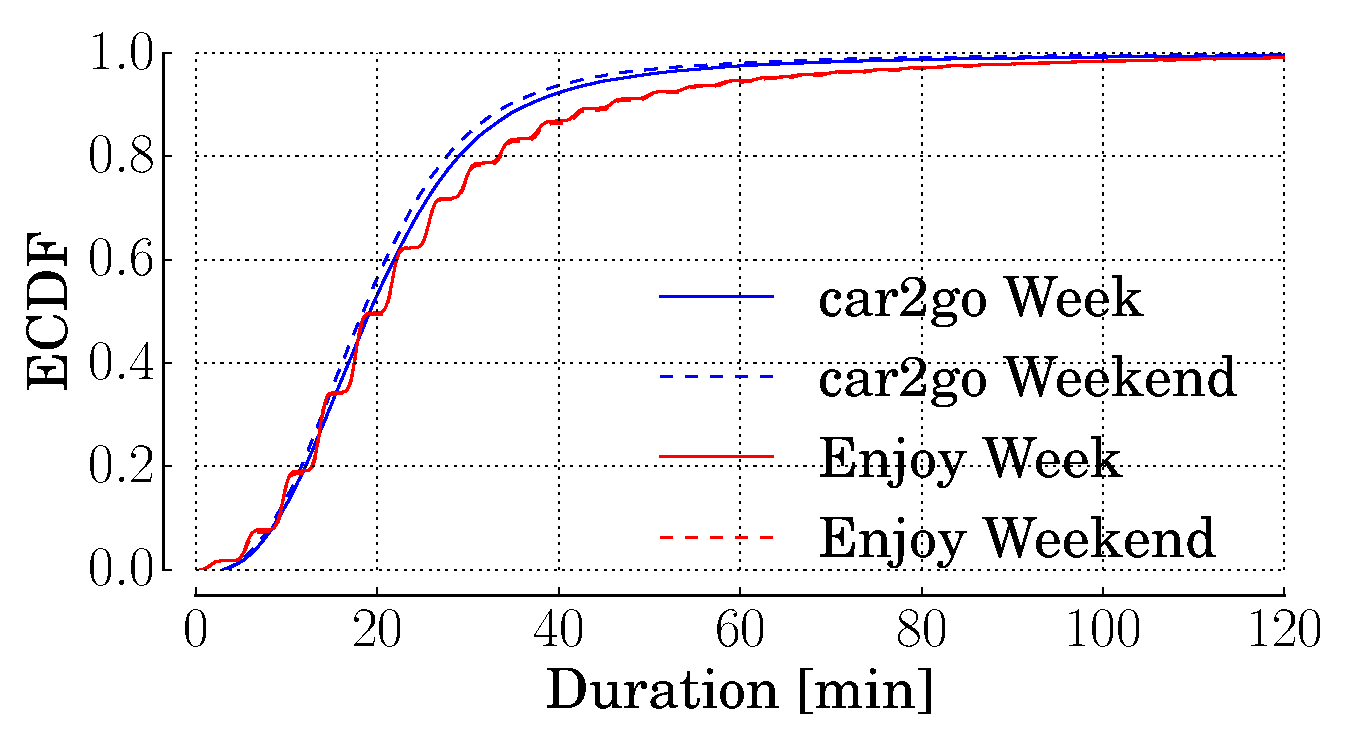
\includegraphics[width=0.33\columnwidth]{figures/duration.pdf}}
%	\subfloat[][ECDF of the rental distance. Weekdays and weekends]{\label{fig:3_5_cdf_distance}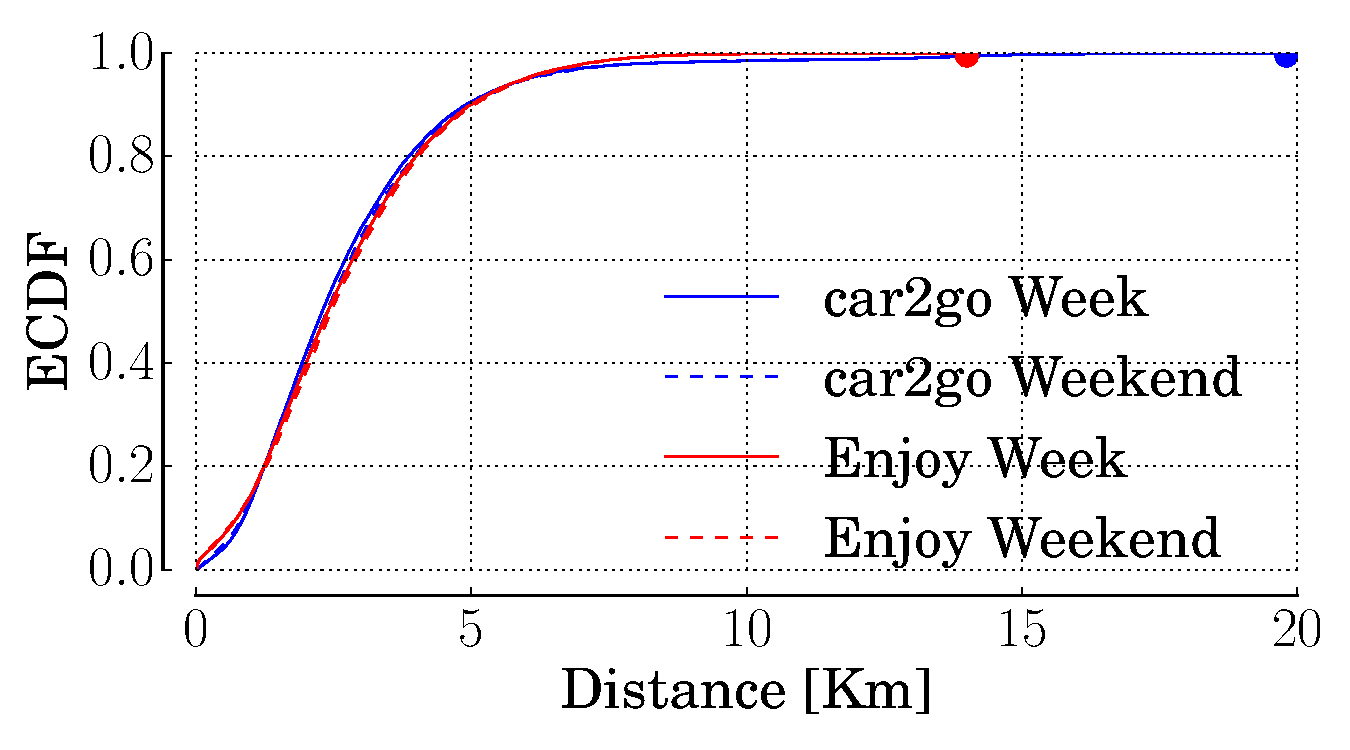
\includegraphics[width=0.33\columnwidth]{figures/distance.pdf}}
%	\caption{Users' booking and rentals habits \mc{magari immagini singole}}
%	\vspace{-3pt}
%\end{figure}


Now, I show how users tend to use FFCS systems during weekdays and weekends. I study three different aspects of users' behaviour: 
\begin{itemize}
	\item for how long users reserve the car before cancelling a booking (Figure~\ref{fig:3_5_pdf_norent})
	\item for how long users rent a car (Figure~\ref{fig:3_5_cdf_duration})
	\item how far users drive (Figure~\ref{fig:3_5_cdf_distance})
\end{itemize}

\begin{figure}
	\centering
	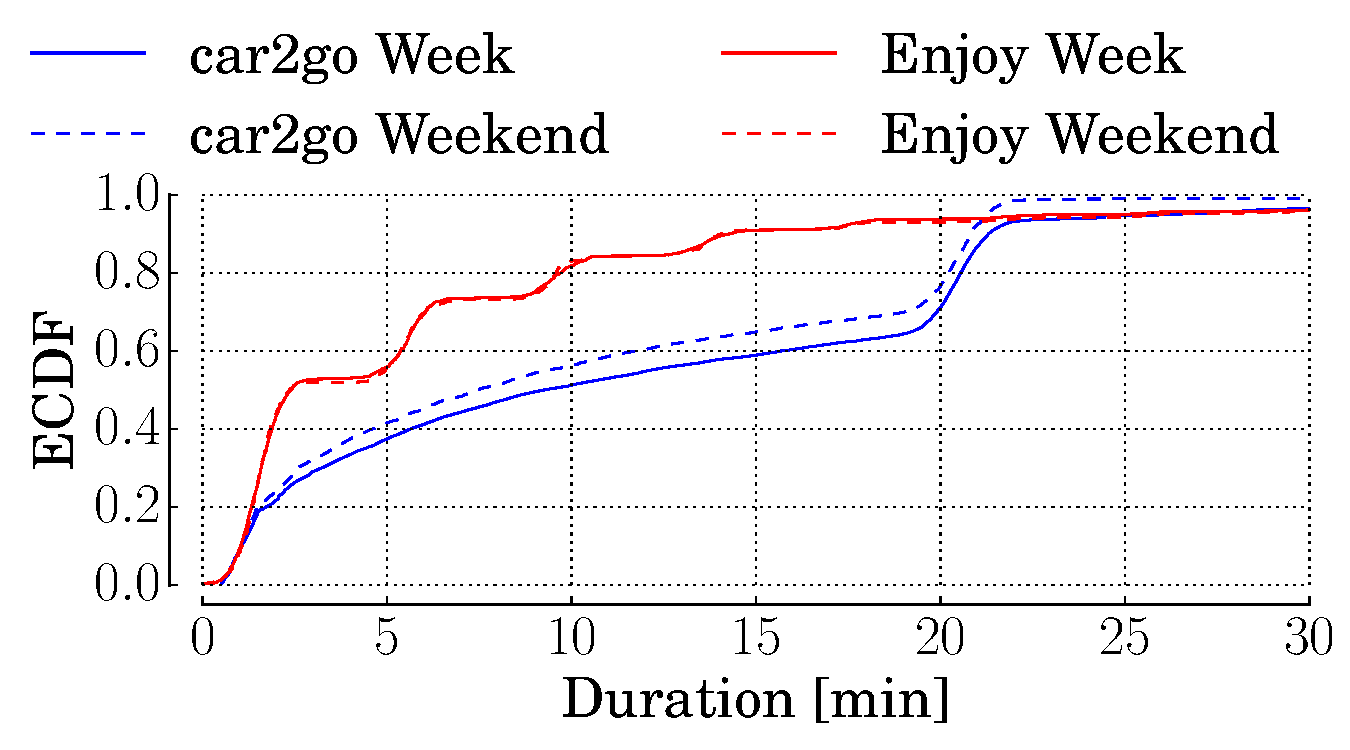
\includegraphics[width=0.85\columnwidth]{figures/no_rent.pdf}
	\caption{ECDF of the booking duration when the booking does not produce a rental. Weekdays and weekends \label{fig:3_5_pdf_norent}}
\end{figure}

First, I check if and for how long users reserve a car and then they cancel a booking. Interestingly, only a small subset of Enjoy bookings are affected by cancellation with respect to car2go bookings. In particular, the dataset presents 14.9\% of car2go and 2.9\% of Enjoy bookings cancellation. This again hints for people preferring to use the Fiat 500 offered by Enjoy, so that they hardly cancel a booking when they reserved an available vehicle. On the contrary car2go availability is higher and so it looks easier to find a closer car. People may thus cancel a previous booking when they find a closer vehicle. Another hypothesis is that car2go may be used as a ``backup'' until an Enjoy vehicle becomes free in the user's area. 

Looking at when people cancel the reservation, figure~\ref{fig:3_5_pdf_norent} shows the CDF of reservation time. Indeed, car2go tends to have a smaller percentage of cancellation within 5 minutes, with a huge step at about 20 minutes. While the first ramp can be explained as a communication error or as some sudden cancellation, the latter can be explained by the \textit{maximum free-of-charge reservation time} of car2go. Truly, users, may reserve a car up to 20 minutes without paying any fee. The same trend is not present for Enjoy which offers a \textit{maximum free-of-charge reservation time} of 15 minutes. Instead, the curve shows a peak at 2 minutes and then a decreasing trend after 15 minutes, when almost all the cancellation are already done.
One last important aspect that this picture shows is how the Enjoy curves have some steps instead of being smooth as the car2go ones. 
This hints to periodic updates on web system so that a time granularity emerges.
To shed some lights on this phenomenon, I performed some active experiments with the Enjoy web portal. The experiment consists of making a new reservation and find when our crawler detects that the car actually disappears from the set of available cars. Then, as soon as I spot the car disappearing, I cancel the reservation to detect when the car reappears in the system. Surprisingly, I discover that when we make the reservation, the car immediately disappears from the system, instead, when I cancel the reservation, the system takes between 1 and 4 minutes to actually show the car again. The presence of such an offset causes the steps in the Enjoy curves which are affected by an artificial delay. To take into account this offset all Enjoy duration have been decreased of 2.5 minutes, i.e., the average delay the Enjoy system adds. 


\begin{figure}
	\centering
	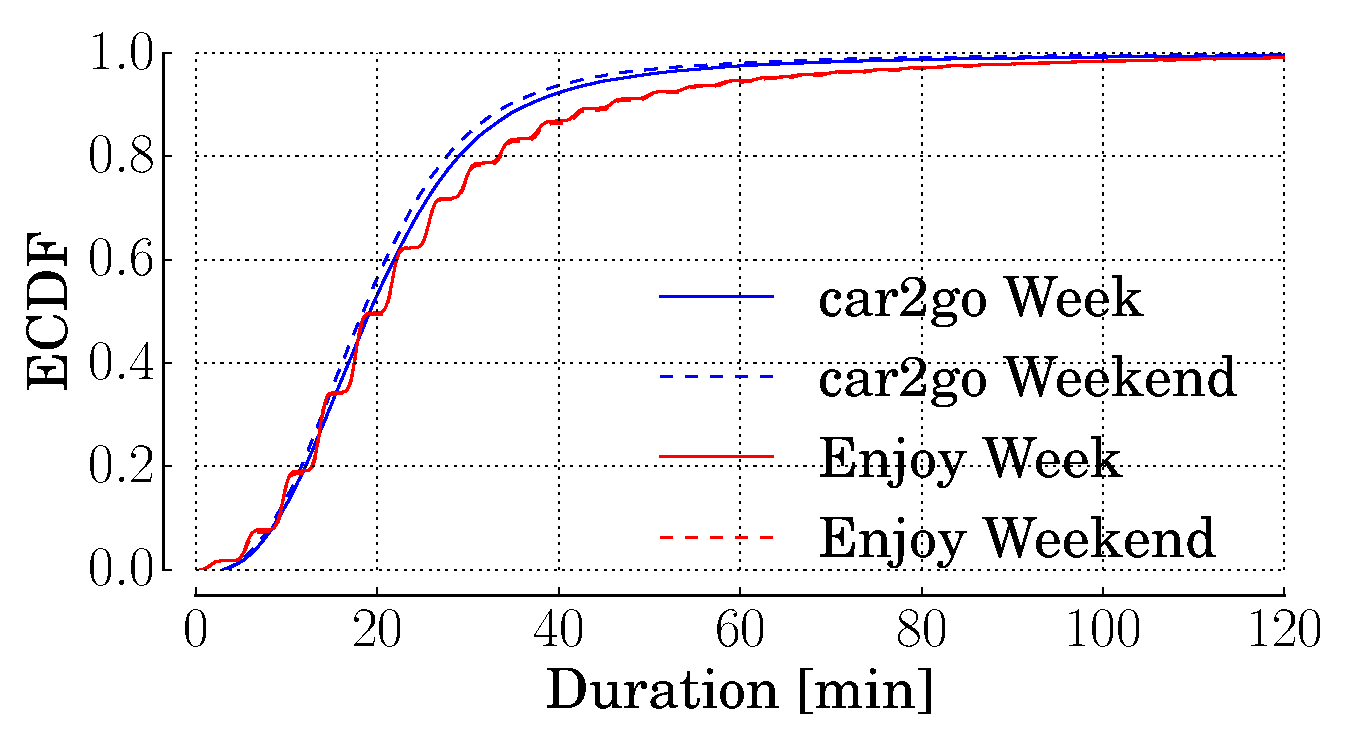
\includegraphics[width=0.85\columnwidth]{figures/duration.pdf}
	\caption{ECDF of the rental duration. Weekdays and weekends\label{fig:3_5_cdf_duration}}
\end{figure}


I next move to characterize the rental duration. Figure~\ref{fig:3_5_cdf_duration} depicts the Empirical Cumulative Distribution Function (ECDF) of the booking duration for Enjoy and car2go during the weekdays and the weekends. The plot shows how the trend tends to be equal during the weekdays and the weekends. This demonstrates that, despite the different pattern of utilization shown before, the booking duration time results similar. Secondly, the ECDFs of car2go and Enjoy are almost overlapped, highlighting how these two services tend to be used in a similar way. Indeed, most of the rentals last less than 1 hour, with 80\% of them lasting less then 30 minutes. It is important to remark that this times include also the reservation time, i.e., the time the user can reserve a car for free before driving it, and the time to find a parking place. Therefore the actual driving time may be significantly smaller.


\begin{figure}
	\centering
	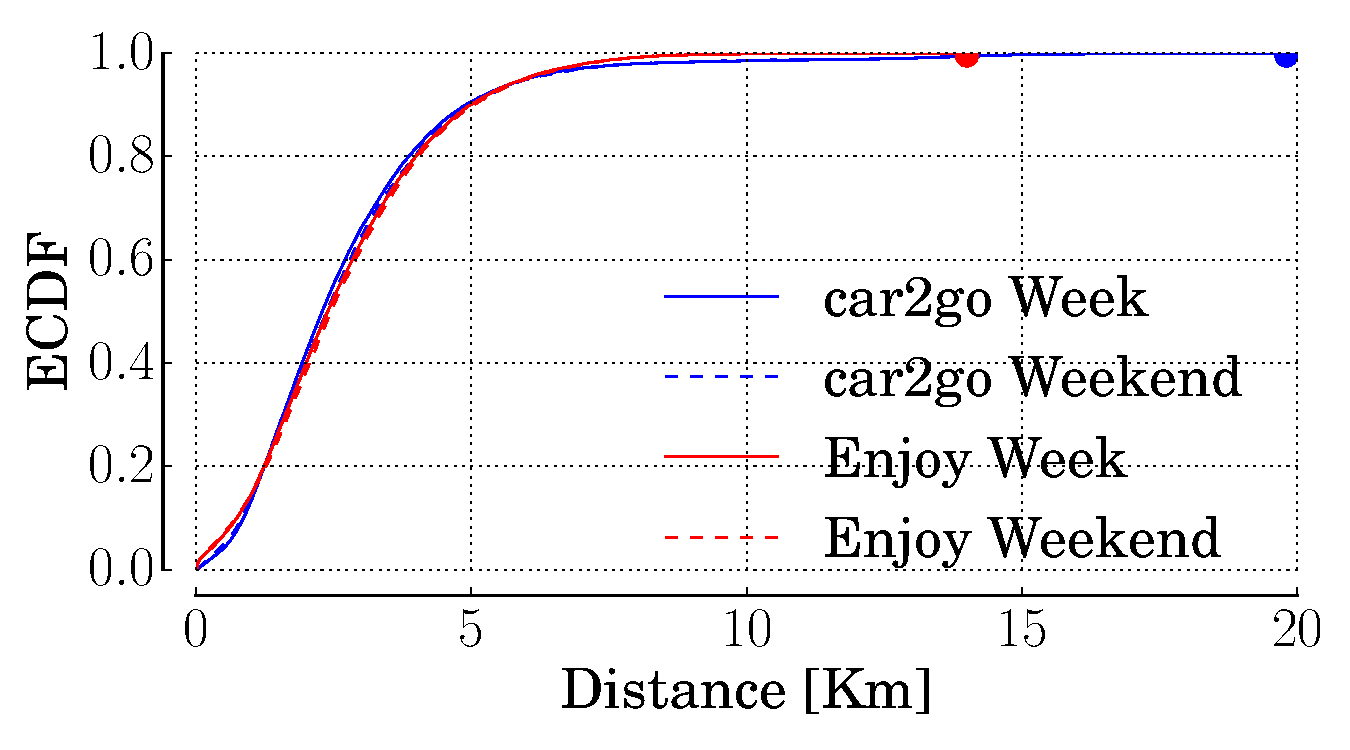
\includegraphics[width=0.85\columnwidth]{figures/distance.pdf}
	\caption{ECDF of the rental driven distance. Weekdays and weekends\label{fig:3_5_cdf_distance}}
\end{figure}


I repeat the same analysis considering the driving distance as reported in Figure~\ref{fig:3_5_cdf_distance}.
To determine the driving distance of each trip we exploit the Google Direction APIs to get the shortest path from the origin to the destination. Similarly, for the driving duration, car2go and Enjoy show a comparable behaviour, and marginal changes during weekdays and weekends. Interestingly, the graphs points out that the 90\% of the trips last less then 5~km demonstrating that most of the rentals are used for short trips both in term of time, and in term of distance. Lastly, the car2go curves saturate many km later than the Enjoy ones as highlighted by the circles. This is due to the possibility to reach the airport of Turin with the car2go cars, which is about 20 km far. 



\begin{figure}[t!]
\centering
\vspace{-10pt}
 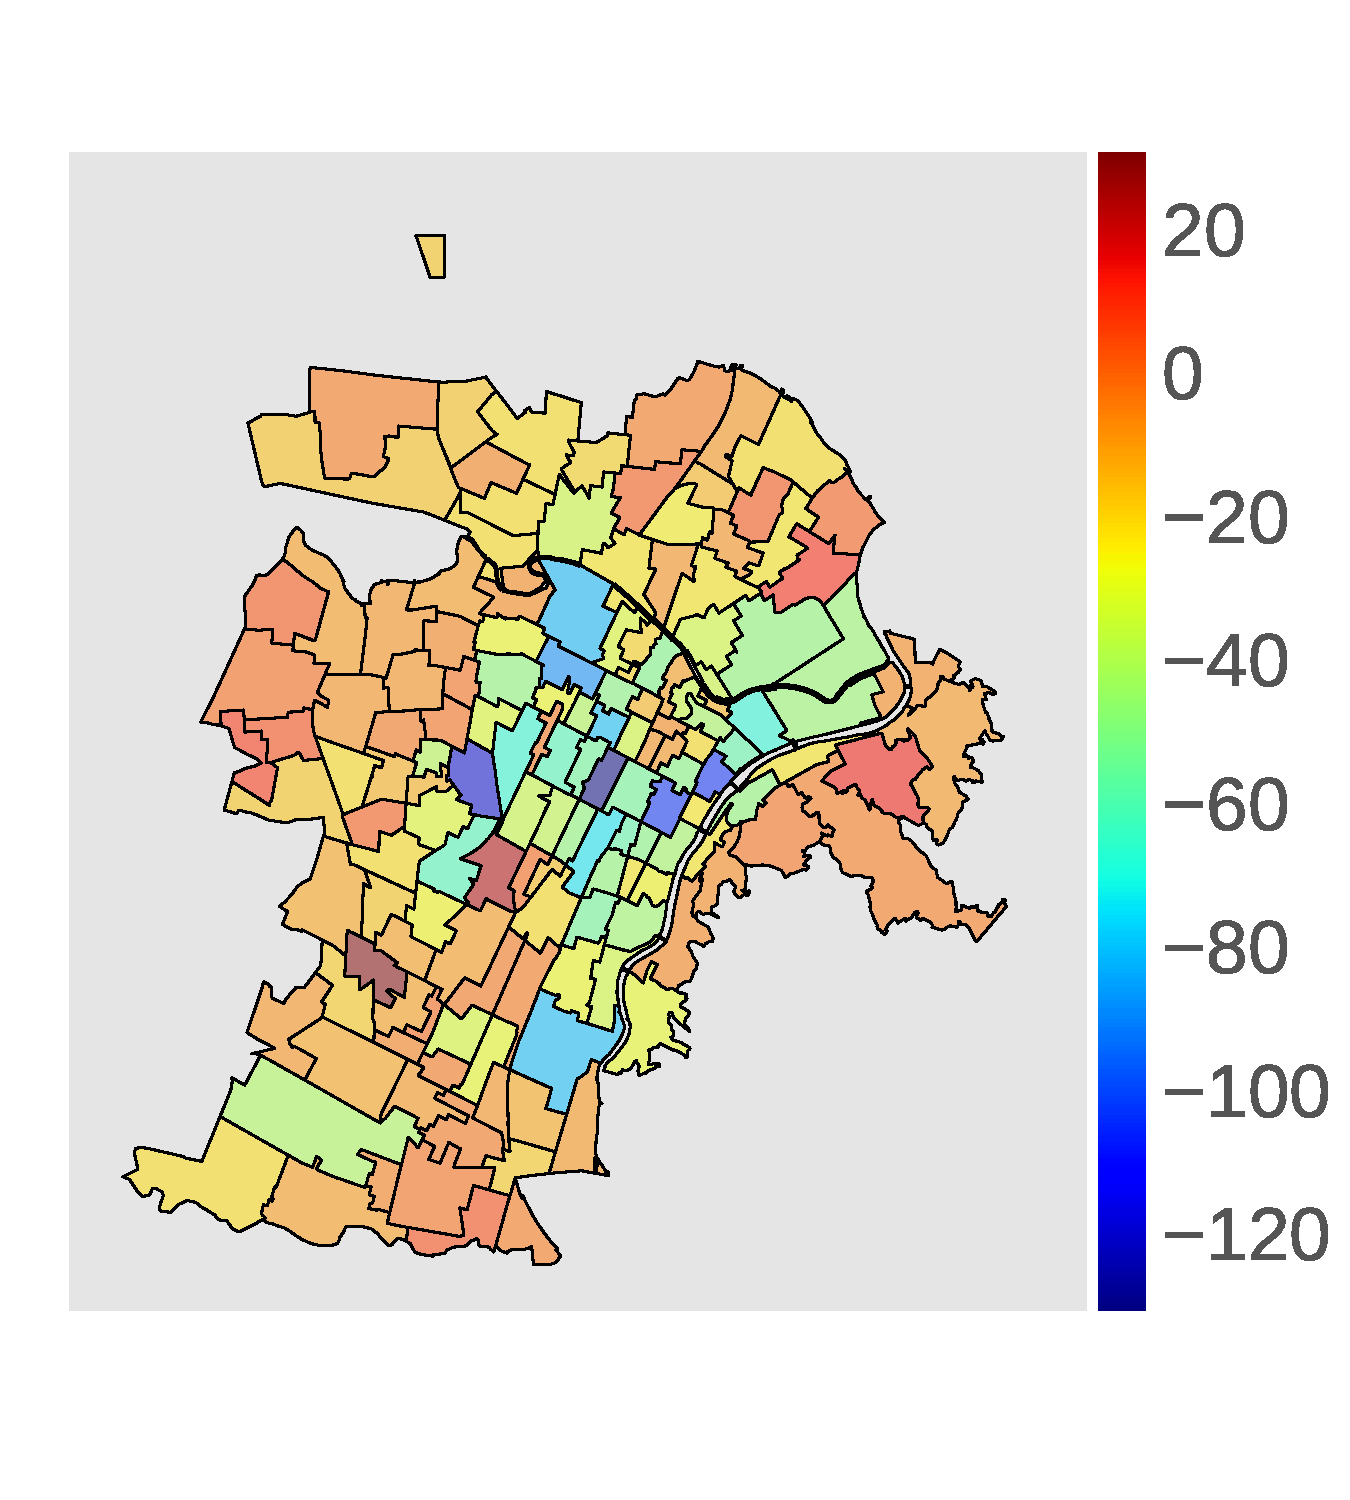
\includegraphics[width=0.72\columnwidth]{figures/clorophlet_o_minus_o1.pdf}
 \vspace{-10pt}
 \caption{Heatmap of arrival - departure per area from 7~am to 12~am vs from 5~pm to 9~pm \label{fig:3_5_heatmap_arr_dep}}
\end{figure}


\subsection{Spatial Analysis}  


In the previous section I analysed car2go and Enjoy only from a temporal point of view. In order to have a complete scenario, it is necessary to study recurrent spatial patterns. To do that I projected the initial and final coordinates on the Turin's neighbour map. Then I computed the attractiveness of each neighbour. Figure~\ref{fig:3_5_heatmap_arr_dep} shows the attractiveness of the  zones in Turin by analyzing the departure and arrival zones. For each zone I compute the difference between bookings ended in the evening [5~pm - 9~pm] and bookings ended in the morning [7~am, 12~am]. Red {areas are those} more attractive during the evening, while blue areas are more attractive in the morning. It is clear that the city center is the most popular destination for car sharing during the office hours, while the trips are sparsely ending in the suburbs during the evening.


\subsection{Users' Habits}

I now characterize how users drive and what is the correlation between public transport usage and availability.

To observe users' driving habits, I use the \textit{driving time} returned by the Google Directions APIs to {obtain} the estimated {driving} time from {rental initial position to the rental final position}. Intuitively, the {rental} time is longer than the driving time as it takes into account also the {reservation} time, and the time to find a final parking spot. Figure~\ref{fig:3_5_heatmap_driving} shows an heat map where the X axis represents the Google estimated driving time and the Y axis the actual booking time. Each cell counts the number of {observed} trips {for each (x,y) pairs}.
For the ease of representation the values are rounded by minute. The diagonal line separates the area where the booking time is lower/greater than the driving time. As expected, most of the trip falls in the area where the booking time is greater then the driving time. However, a non negligible number of trips (12.1\%) falls in the area where the booking time lasts less than the driving time. 

\begin{figure}[h!]
	\centering
	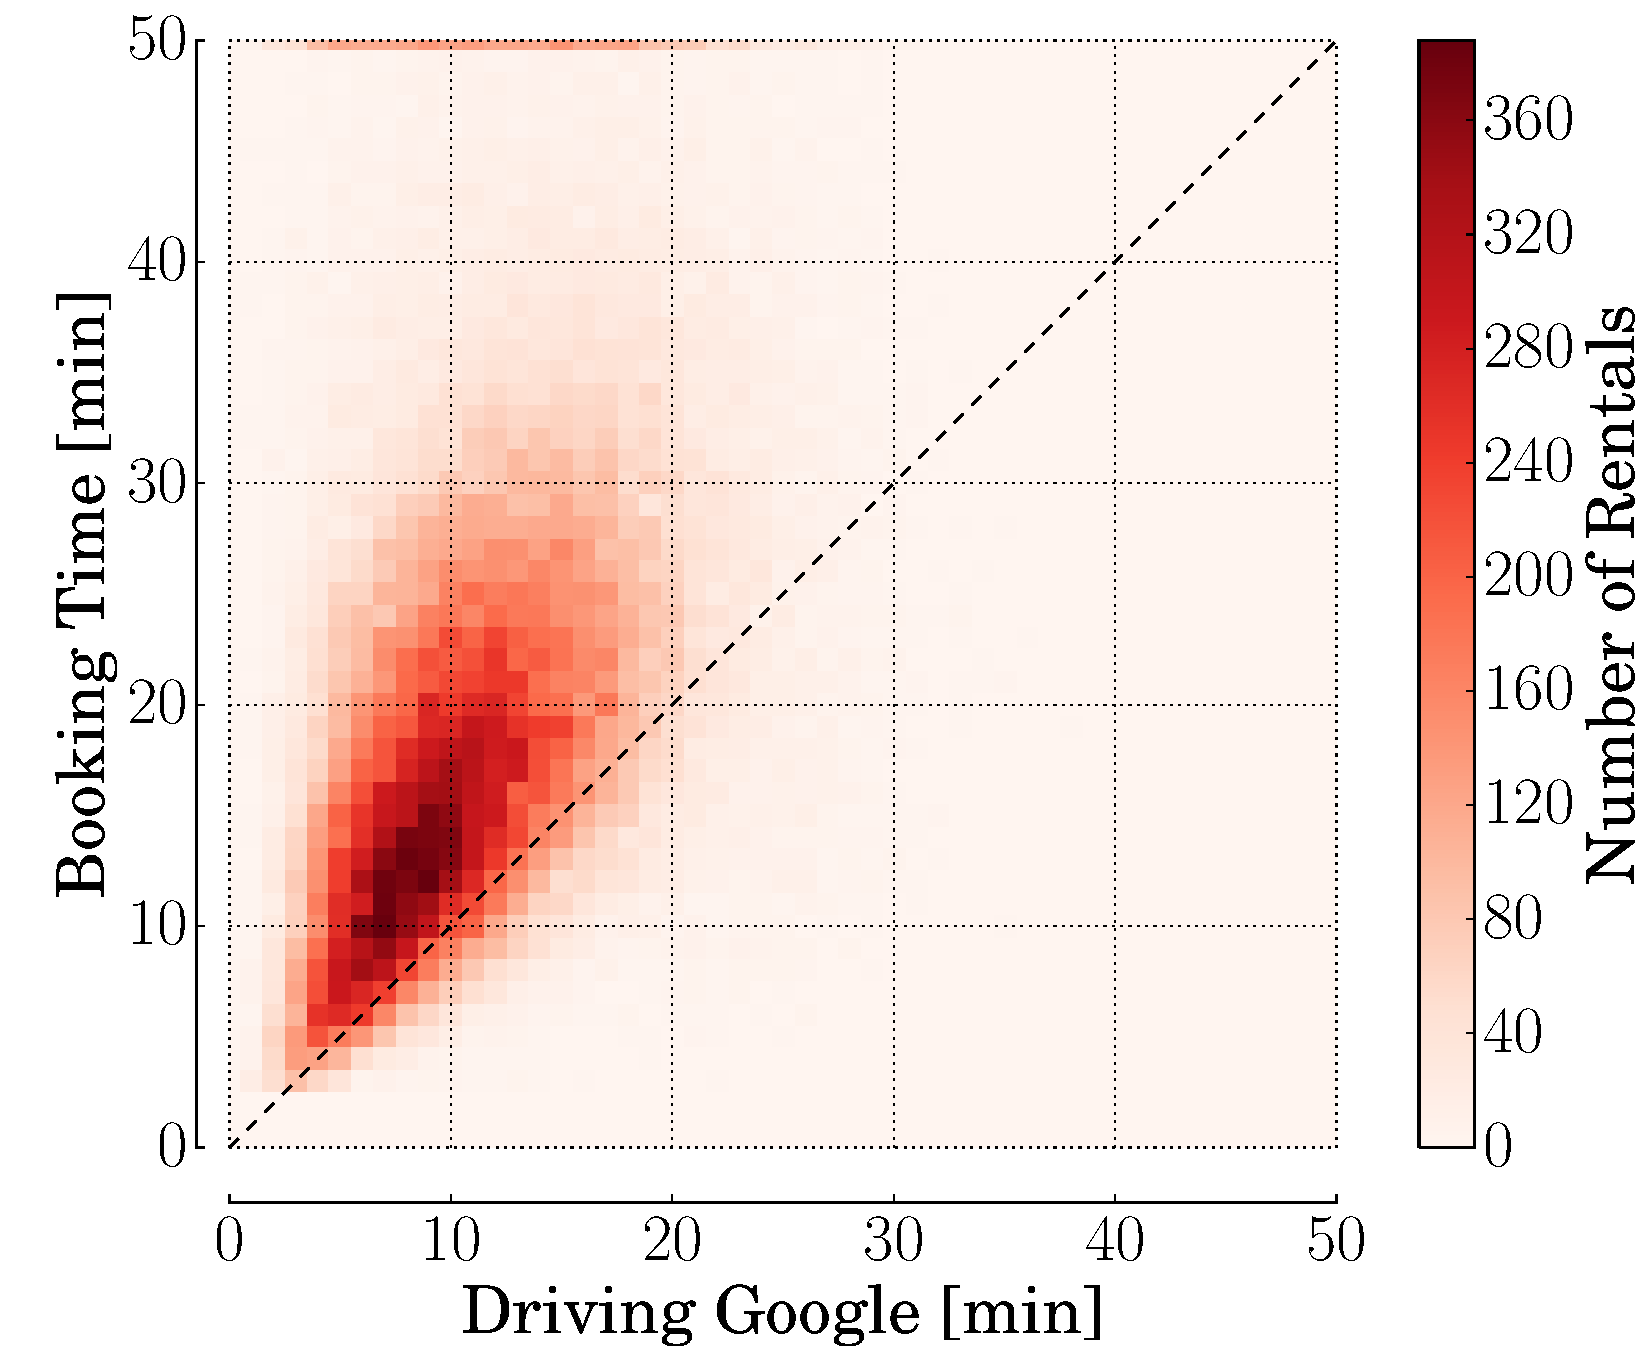
\includegraphics[width=0.85\columnwidth]{figures/car2go_faster_driving.pdf}
	\caption{Heatmap of booking time vs estimated driving time by Google\label{fig:3_5_heatmap_driving}}
\end{figure}


This may be due to several factors: Google Directions possibly overestimating the average trip duration, or users driving faster than expected.
To better quantify how much faster users drive the car in those cases, I  computed the difference between the driving time and the actual booking time. I show the Empirical Cumulative Distribution Function of such values in Figure~\ref{fig:3_5_cdf_faster_google}. It is possible to see that te most of these trips are only 5 minutes faster than the estimated driving time, with Enjoy users which seems to drive faster than car2go ones. Indeed, if the trip is more than 10 minutes faster, Google suggested a longer path to the destination, e.g., suggesting to take the highway which was much longer with respect to crossing part of the city.

This analysis hints that the current pricing policy, which depends only by the booking time, may have some drawbacks as it may encourage users to drive fast. An hybrid pricing policy, which takes into account both the time and the distance, may be effective in solving this problem, e.g., by increasing the price in case of an user drive faster than expected, or by reducing the fee in case of traffic congestion.

\begin{figure}[h!]
	\centering
	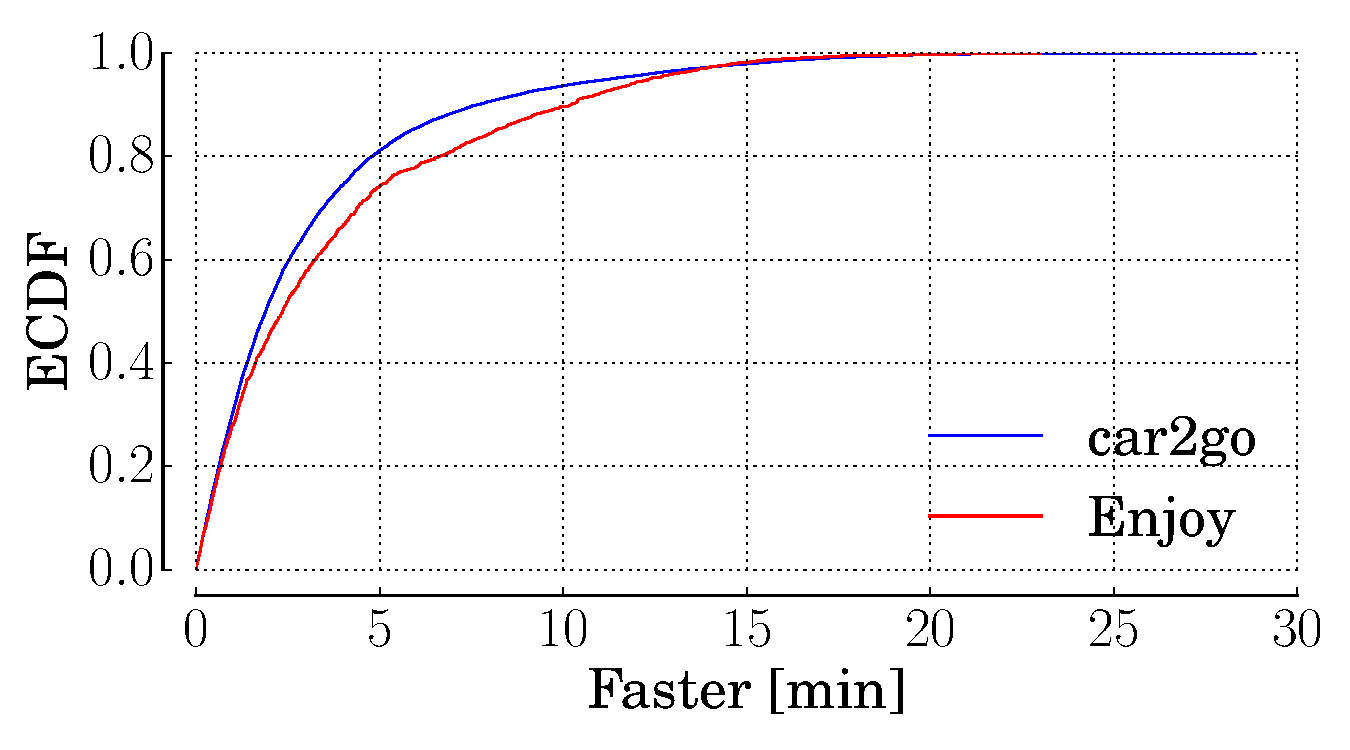
\includegraphics[width=0.85\columnwidth]{figures/faster_driving.pdf}
	\caption{ECDF of the difference between the expected driving time and the actual driving time\label{fig:3_5_cdf_faster_google}}
\end{figure}


%\begin{figure}[t!]
%\centering     %%% not \center
%\subfloat[][Heatmap of booking time vs estimated driving time by Google]{\label{fig:heatmap_driving}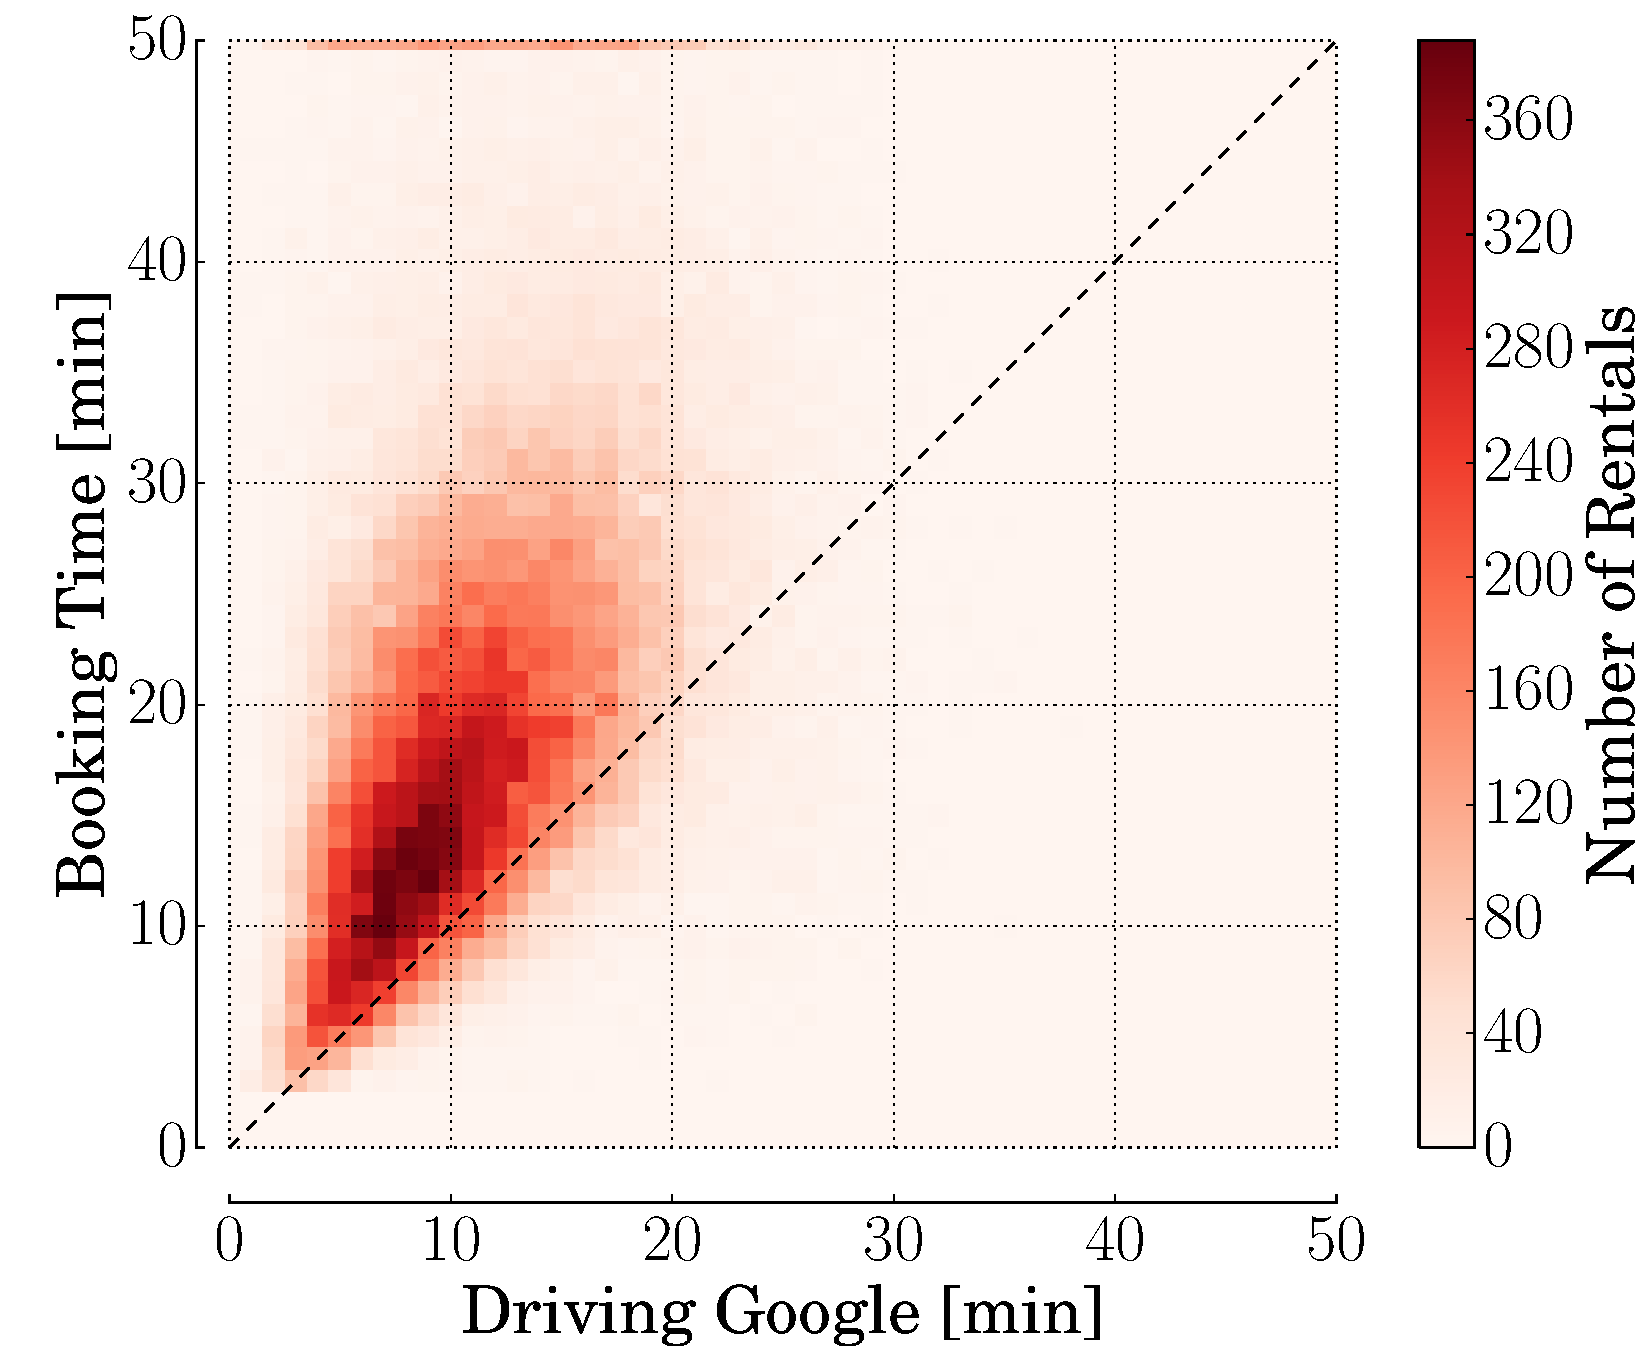
\includegraphics[width=0.5\columnwidth]{figures/car2go_faster_driving.pdf}}
%\subfloat[][ECDF of the difference between the expected driving time and the actual driving time]{\label{fig:cdf_faster_google}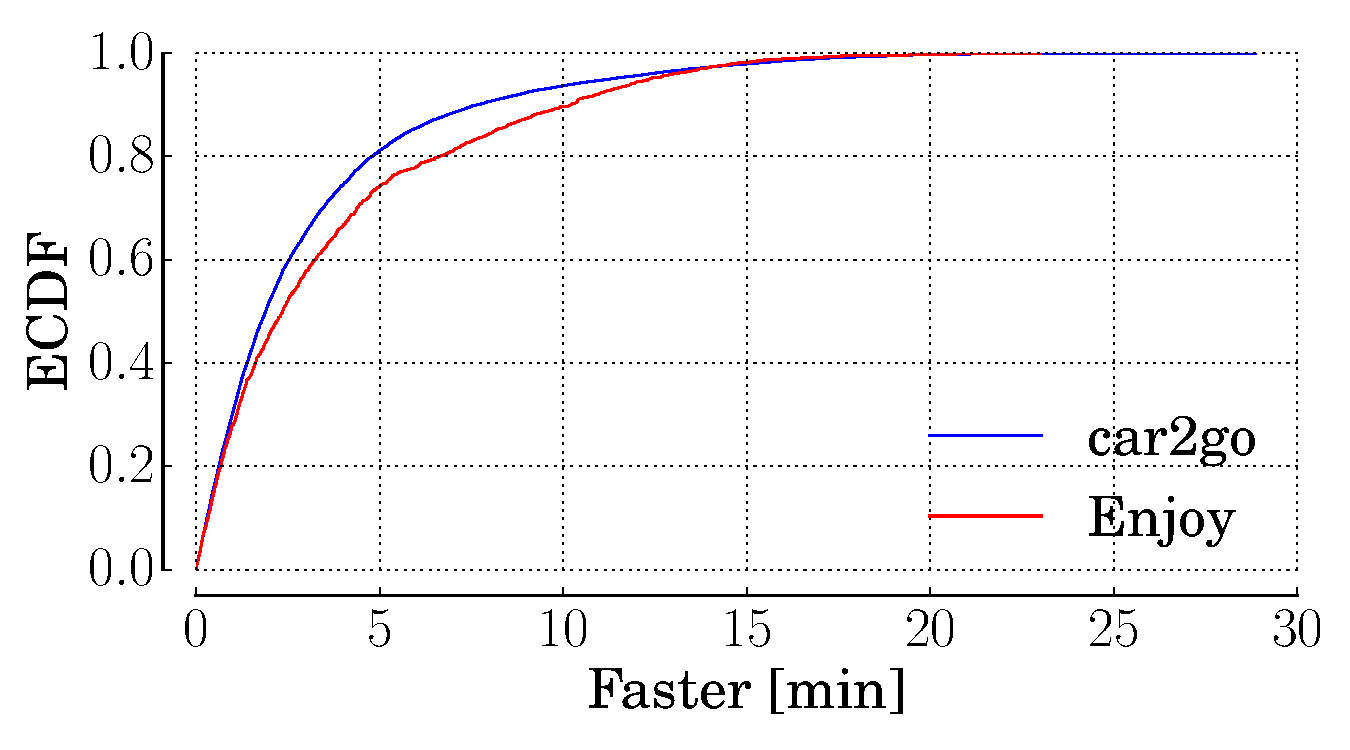
\includegraphics[width=0.5\columnwidth]{figures/faster_driving.pdf}}
%\caption{Users' driving habits}
%\end{figure}


At last, I leverage Google Directions APIs to extract public transport travel information for each vehicle's trip. I want to analyse another way of mobility in the urban area, and compare car sharing usage with respect to public transport. Results are shown in Figure~\ref{fig:3_5_public_transport}.
%The public transport duration includes both the time of travel and time of wait.
As one could expect, the majority of trips last less than public transport. The higher density is for bookings that last between 10 and 20 minutes. For longer trips, the discrepancy in terms of duration is higher, probably due to the longer path and the higher number of stops of the public transport. Conversely, I can interpret the points where the booking time is greater than  the public transport duration as trips where the customers spent a lot of time in reaching the car or finding a parking spot for the drop-off.

\begin{figure}[h!]
	\centering
	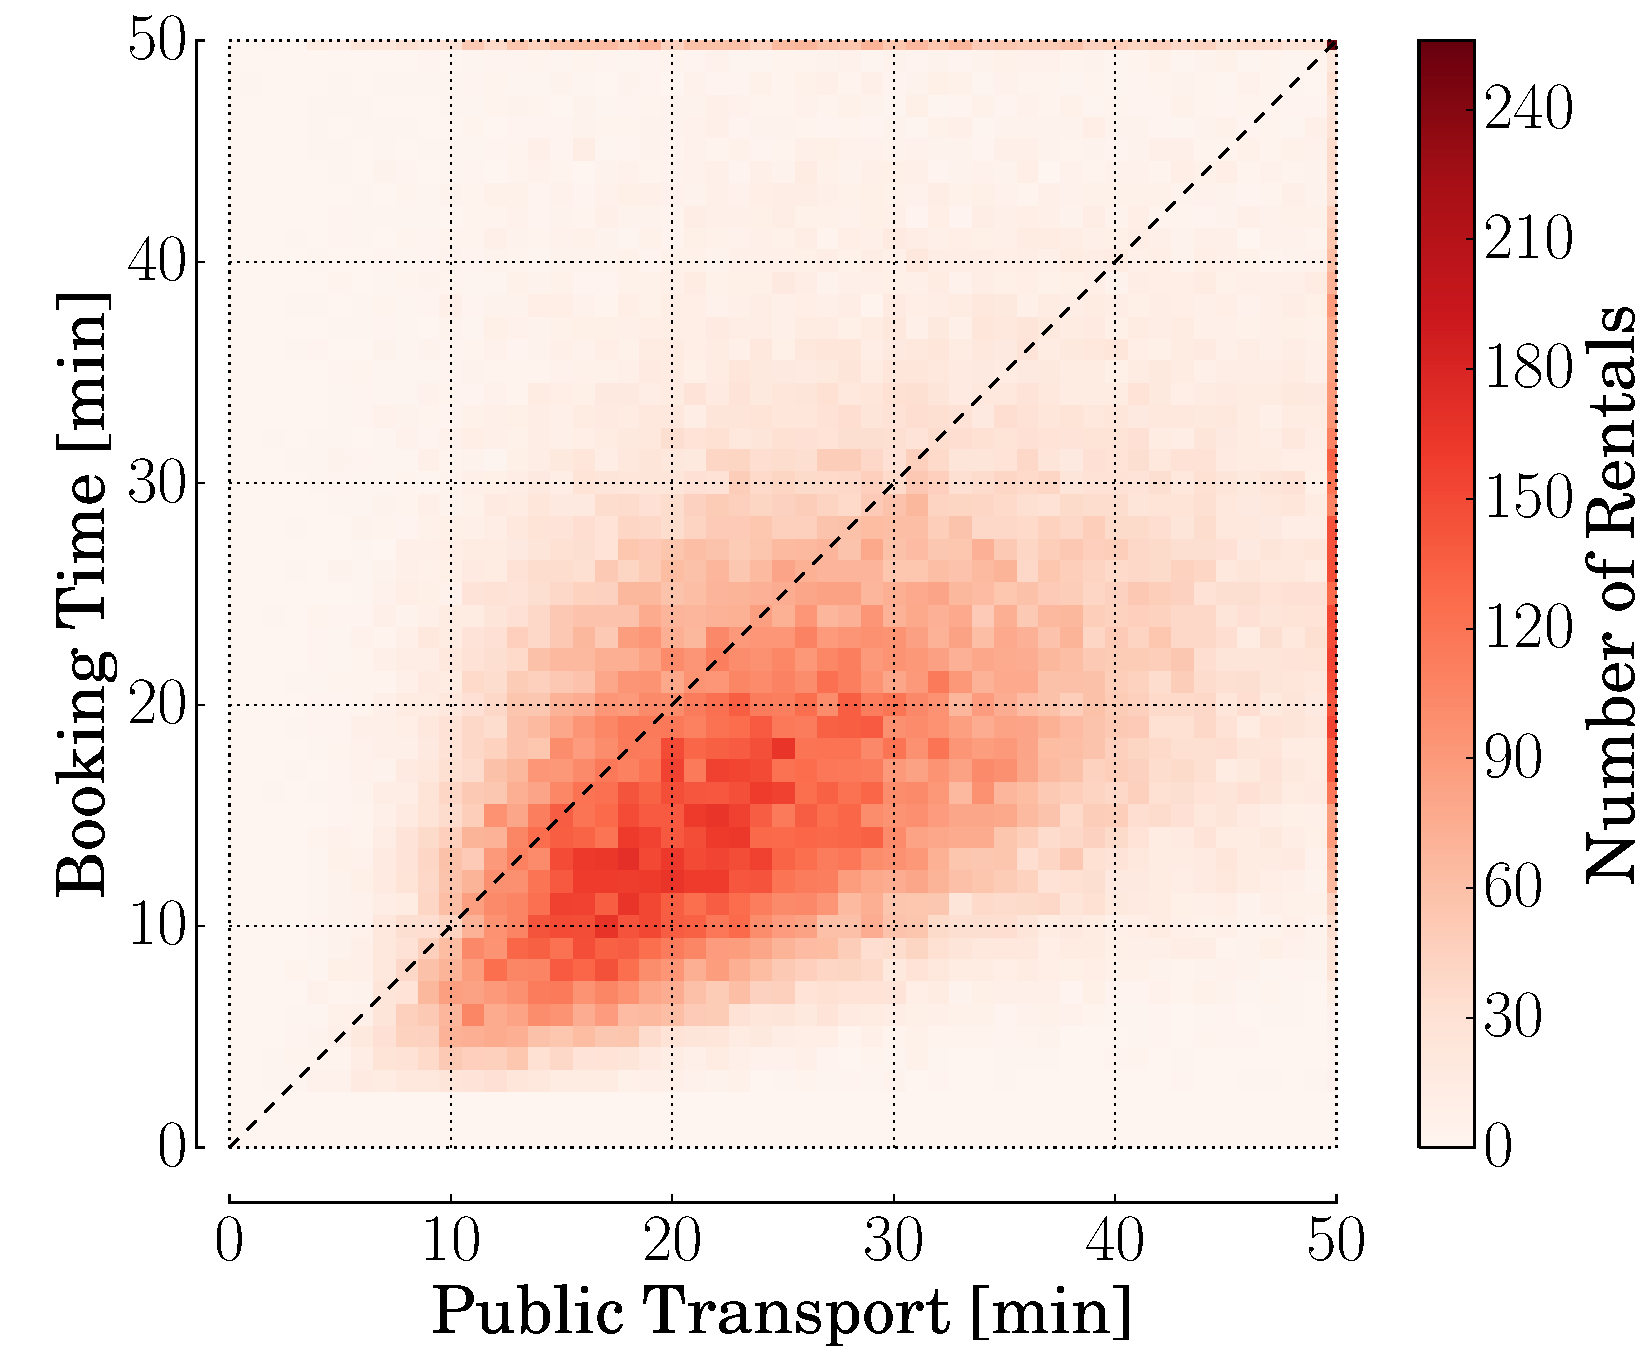
\includegraphics[width=0.85\columnwidth]{figures/car2go_faster_public.pdf}
	\caption{heatmap of the booking time  vs the estimated public transport time by Google\label{fig:3_5_public_transport}}
\end{figure}

To help to visualize the juxtaposition of car sharing and public transport, we extract from the data the probability of booking a car, conditioned to the public transport travel time. Figure~\ref{fig:pdf_transport}, reports on the X axis the public transport duration (as predicted by Google) in intervals of 5 minutes, and on the Y axis the probability of booking a car for each interval.
The distribution of probability is similar for both car2go and Enjoy. Higher values are reported for trips that can be covered by public transport between 15 and 35 minutes. Interestingly, car sharing mobility is not preferred for very short trips, while the distribution shows a significant tail for duration greater than 30 minutes. This behavior can be justified by the significant amount of time that can be saved with cars haring with respect to public transport.

\begin{figure}[h!]
	\centering
	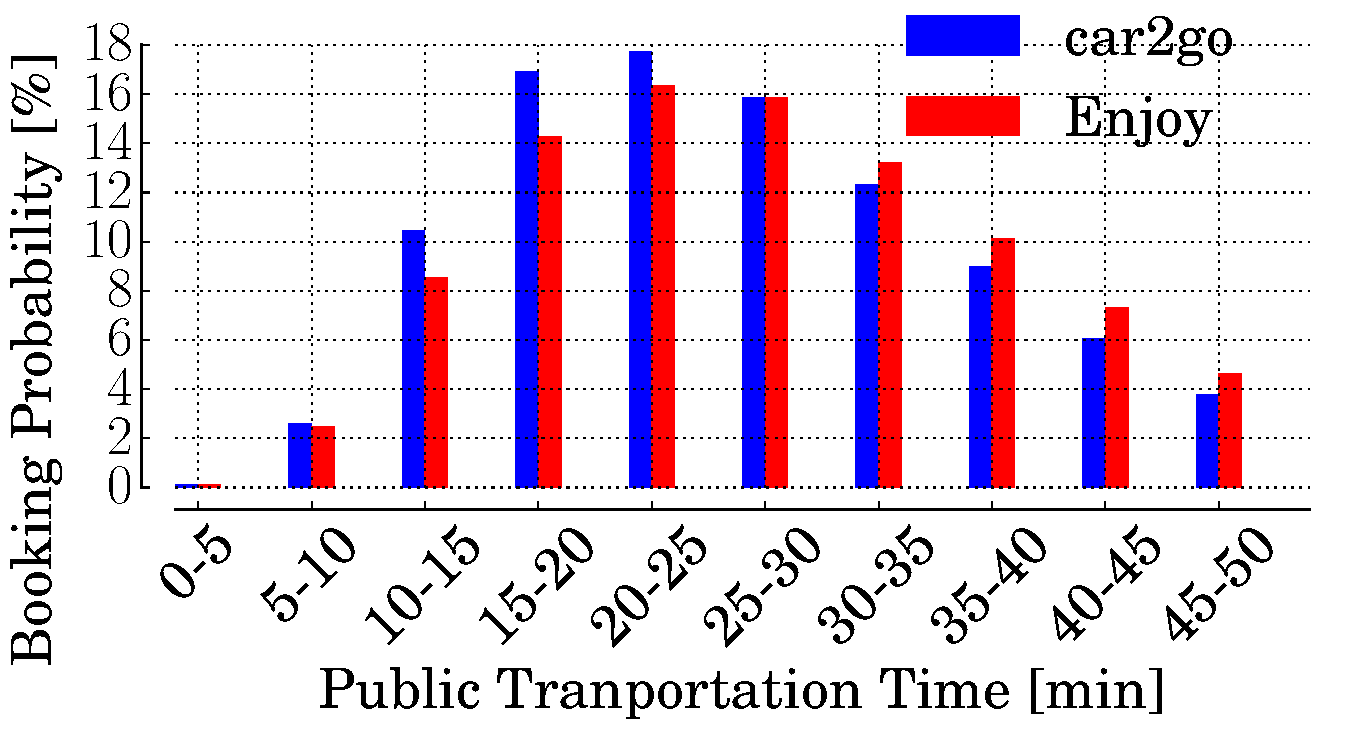
\includegraphics[width=0.85\columnwidth]{figures/public_tranport_probability.pdf}
	\caption{Public transportation vs car sharing\label{fig:3_5_public_tranport_probabilityt}}
\end{figure}
  
%  \begin{figure}[t!]
%  \centering     %%% not \center
%  \subfloat[][heatmap of the booking time  vs the estimated public tranport time by Google]{\label{fig:heatmap_transport}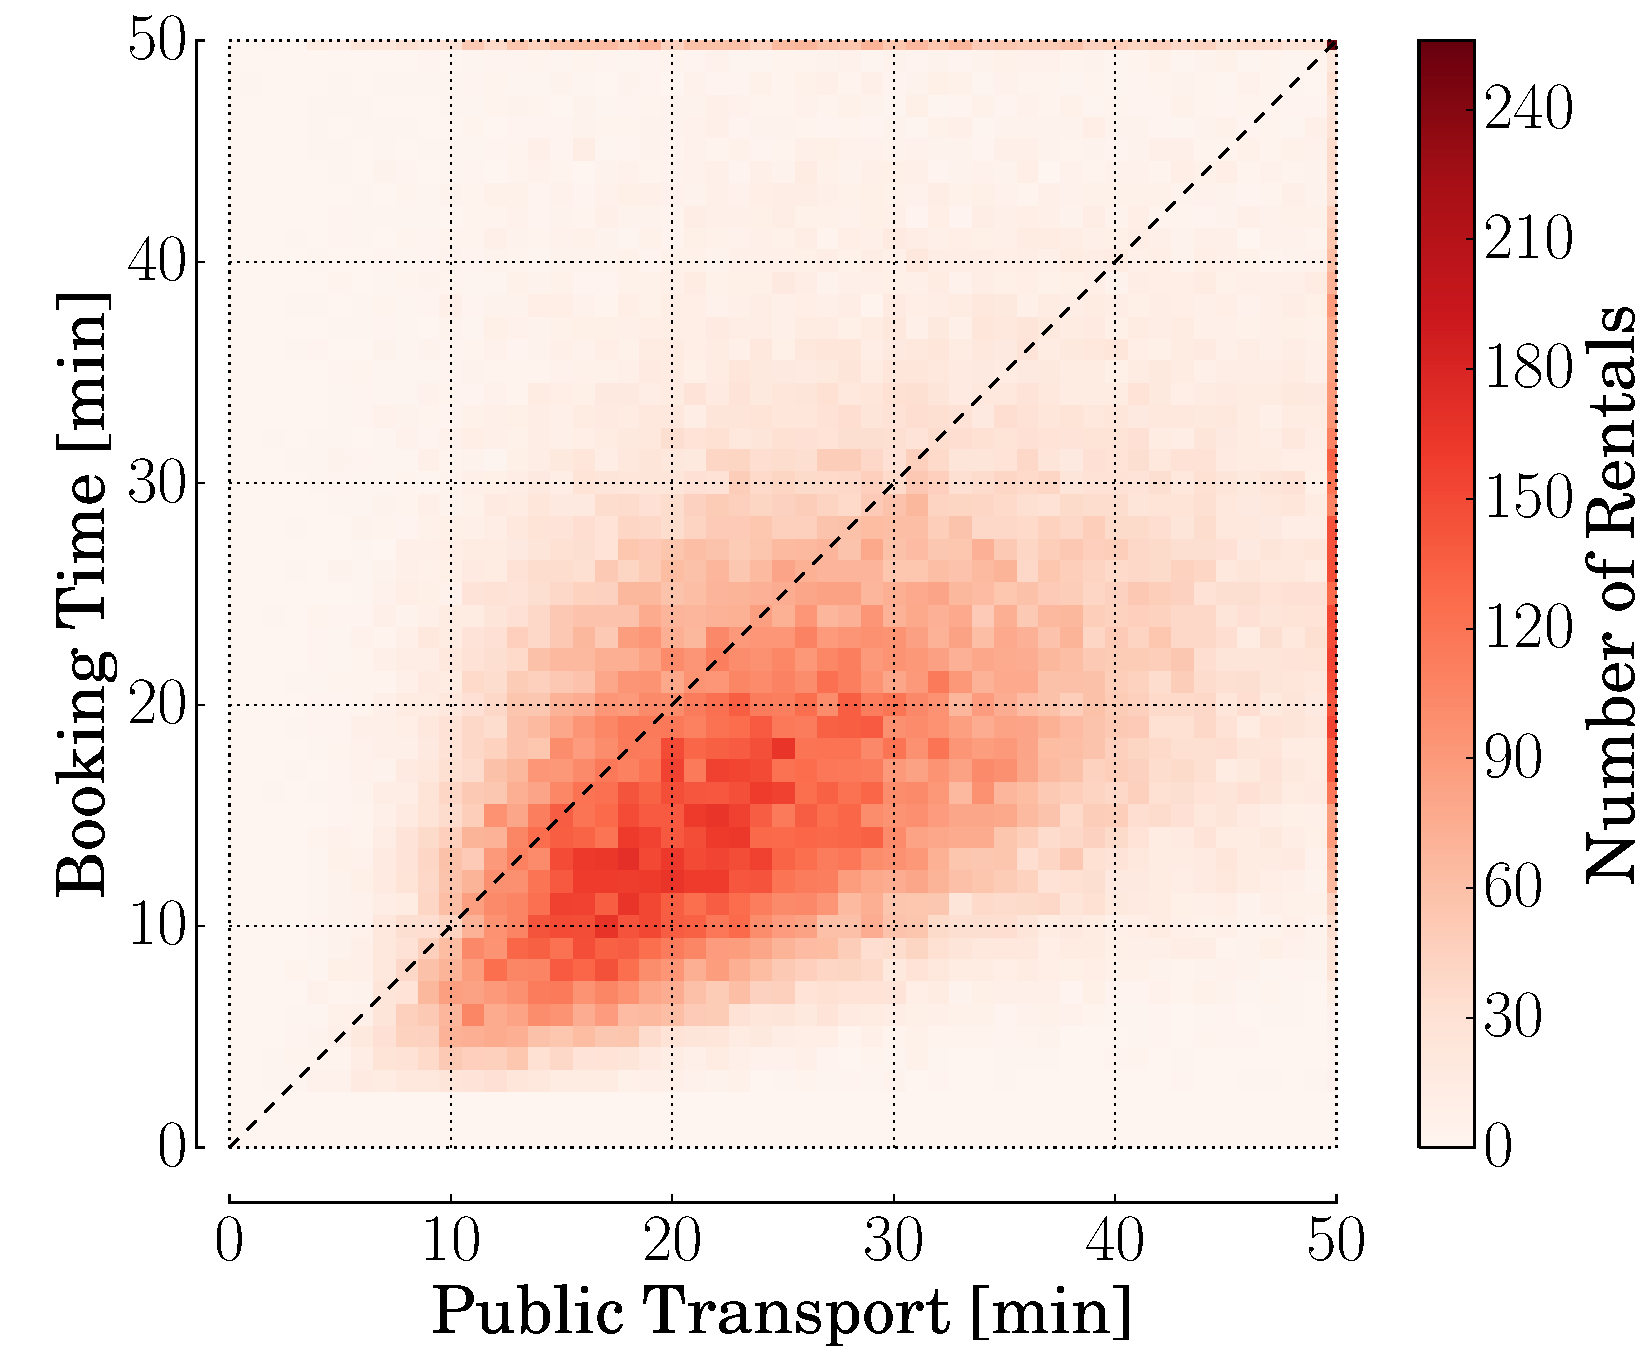
\includegraphics[width=0.5\columnwidth]{figures/car2go_faster_public.pdf}}
%  \subfloat[][Probability of using car sharing based on public transport time by Google]{\label{fig:pdf_transport}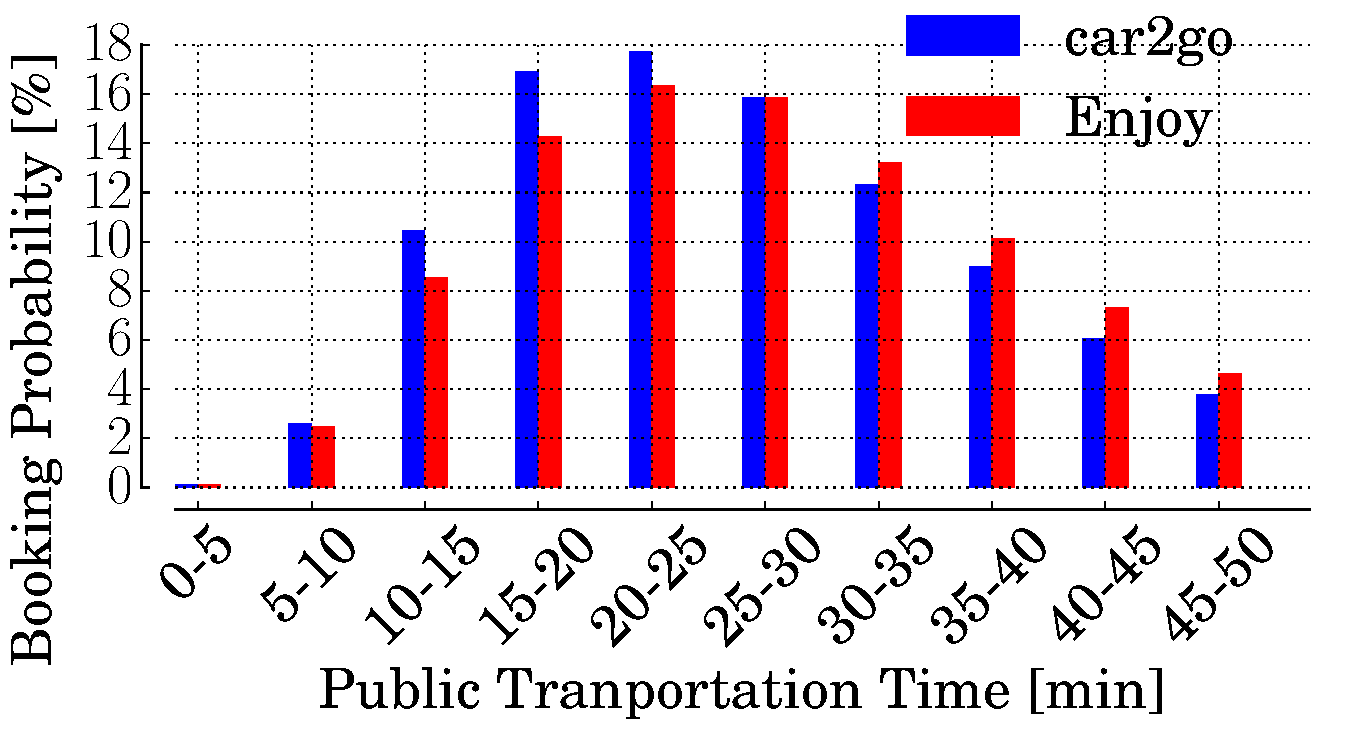
\includegraphics[width=0.5\columnwidth]{figures/public_tranport_probability.pdf}}
%  \caption{Public transportation vs car sharing \label{fig:public_transport}}
%  \end{figure}
%  
  
 
Finally, to globally understand how users tend to use the different services we report in Figure~\ref{fig:avg_comparison} the average time for: the Enjoy rentals (red curve), the car2go bookings (blue curve), the driving time (green curve), and public transport time (orange curve). To compute this value, for each hour we take all the rentals of interest, and then we compute the average value and report it. A first interesting aspect is that the average time of Enjoy is always greater then the car2go ones and for the pure driving time. Secondly, both show a similar trend with, a decreasing average duration during the night. As a consequence, it is unjustifiable ascribe this trend with traffic jam, instead, but more likely with an increase time in the reservation time and in the parking time. Finally, it is possible to appreciate how during the night the public transport takes more than 1 hour for trips which last less then 20 minutes by car. Instead, during the daytime the average public transport time get close to the car sharing time. 
%This demonstrates the goodness of the public transport system.



\begin{figure}[h!]
\centering
 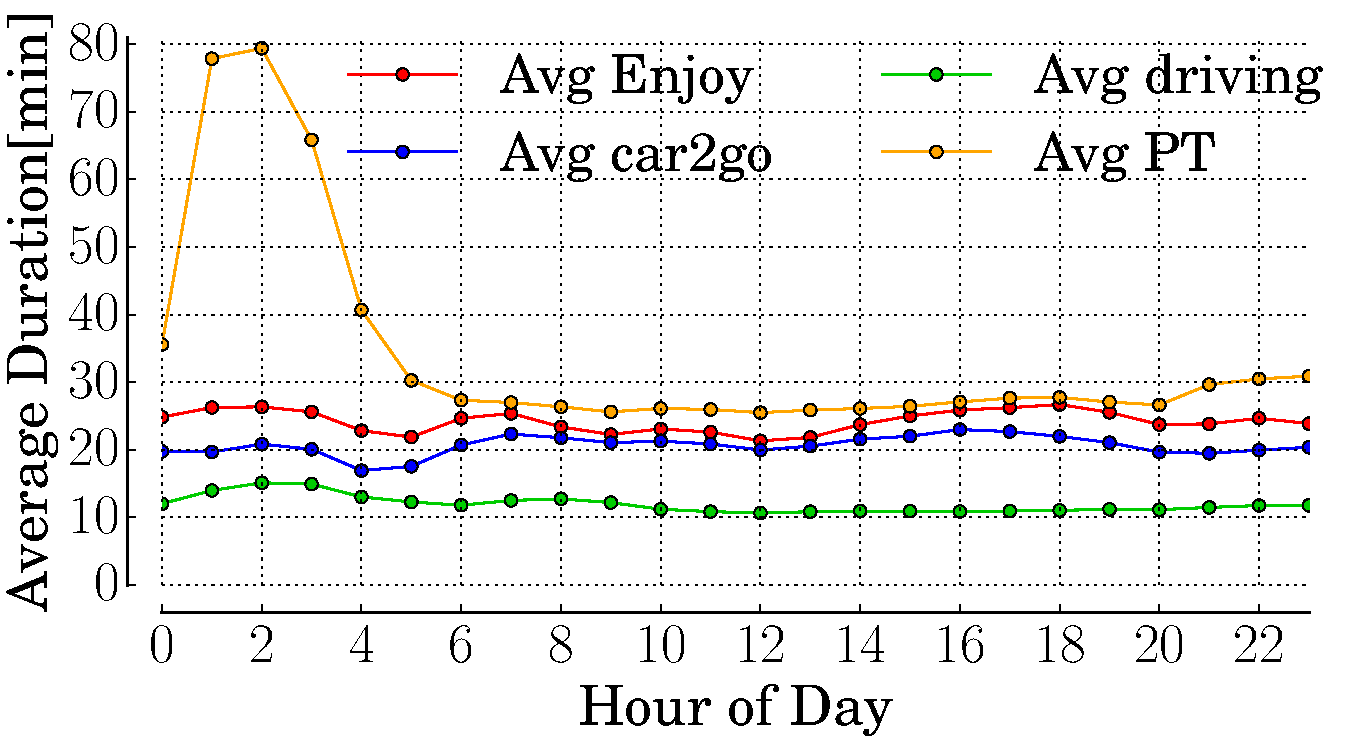
\includegraphics[width=0.85\columnwidth]{figures/average_duration.pdf}
 \caption{Average Time per transport solution per hour \label{fig:avg_comparison}}
\end{figure}



%\section{Conclusions}
\label{sec:3_conclusion}

In this chapter, I presented some analyses made possible through \tool, a platform I designed and described in chapter \ref{chap:2_dataset} to collect and store data, and able to extract higher level information from FFCS provider.

By analyzing the data, I highlighted different aspects related to the system utilization, how users move in the city in different periods of the day, and what are the users' driving habits.

This analysis demonstrated the big amount of information that it is possible to extract from well designed data collection pipelines. Indeed,  by looking the system utilization, I demonstrated that FFCS cars are frequently used for short trips which last less then 30 minutes and 5 kms. Moreover, despite Enjoy has a smaller fleet, its system utilization is frequently higher than car2go one due to the more appreciated car model it offers. Exploiting the spatial analysis, I highlighted how users tend to move during different time periods. Finally, the users' driving habits showed us that current charging policy may encourage users to drive fast. 


% !TEX root = ../toptesi-scudo-example.tex
% !TEX encoding = UTF-8 Unicode
%***********************************************************************
%***********************************Third Chapter
%***********************************************************************

\chapter{CS comparison}
\label{chap:4_cs_comparison}
	\graphicspath{{Chapter4/}}


\section{Abstract}
\label{sec:3_0_abstract}

The understanding of the mobility on urban spaces is useful for the creation of smarter and sustainable cities. However, getting data about urban mobility is challenging, since only a few companies have access to accurate and updated data, that is also privacy-sensitive. 

In this work, we characterize three distinct car-sharing systems which operate in Vancouver (Canada) and nearby regions, gathering data for more than one year. Our study uncovers patterns of users' habits and demands for these services. 
We highlight the common characteristics and the main differences among car-sharing systems. Finally, we believe our study and data is useful for generating realistic synthetic workloads.

\section{Introduction}
\label{sec:4_1_intro}

Urban mobility is a key research area, attracting several academic studies and private investments. It is intrinsically connected to a wide number of urban activities, such as the demand for communication resources. Understanding the urban mobility, specifically the traffic-related mobility with motorized vehicles, is currently acquiring more importance, in order to improve the people quality of life studyng for example road mesh planning and communication resources allocation~\cite{herrera:10, Ma:2013}.

The first step in understanding urban mobility patterns is the proper acquisition of data. Data can be obtained in several ways, e.g., by observing vehicles passing through sensors or fixed/mobile radars, by acquiring traffic data from cameras, or by the active participation of users (\textit{crowdsourcing}). However, large and heterogeneous data acquisition is still a challenge. Indeed, only a few companies have access to them and usually, they embed some random components to protect the users' privacy ~\cite{ciociolaumap}. Therefore, it is important to collect and study the available open data and generate models that can help to understand the urban mobility and the social interactions of people in the urban environment.


Many alternative transport modes contribute to urban mobility. Among them, the car-sharing paradigm is quickly growing~\cite{boldrini:16,ciociolaumap,becker2017comparing}. In a car-sharing system, people can drive a vehicle, without worrying about buying it and paying for maintenance, fuel and parking fees. %These systems have already a significant volume of users and thus are an important type of urban mobility pattern. In fact,
By 2015, more than 1.5 million users and 22\,000 shared vehicles have been counted in the Americas, and growth in usage is still expected~\cite{shaheen2016mobility}. 
Overall, car-sharing services are classified into three categories: 
\begin{itemize}
		\item the one-way services, where the vehicles are available in specific stations and the user can move a car from a station to another
		\item the two-way services, where the user must return the vehicle to the same station she/he picked up the vehicle and;
		\item the free-floating service where vehicles are not tied to stations. In this case, the users are able to start and finish their trips everywhere within an operative area and in public parking spots~\cite{boldrini:16}
\end{itemize}. 

This chapter proposes a comparison between free floating and different station based car sharing paradigms. More in details we characterized those services in order to outstanding different users' habits. We take as case of study the city of Vancouver that hosts, several car-sharing providers. Our characterization relies on data we gathered for more than a year from Modo, Evo and Car2Go \footnote{service dismissed on February 29, 2020} car-sharing services ---a two-way, a one-way and a free-floating service, respectively---.
The chapter illustrates the users' demand and usage patterns of vehicles from these services and, at a glance, the contributions are twofold: first, a characterization of three important car-sharing paradigms and, second,  a demand model for their vehicles, providing statistical distributions which describe their busy and idle periods. 
This study is important to highlight particular situations where car-sharing services are attractive and, together with data from other transport modes, to uncover trends and mobility patterns. Moreover, we also believe the collected data and the developed models can be used to generate accurate synthetic workload. As a consequence, these can contribute to the development of better capacity planning models to car-sharing systems and also to a better plan of public transport systems.
%To best of our knowledge, we are the first to jointly consider all these three types of services, leveraging their common characteristics and highlighting their peculiarities.


The remainder of this chapter is structured as follows:  Section \ref{sec:4_5_related} describes related work; Section \ref{sec:4_2_carsharing} describes details of the three car-sharing paradigms; Section \ref{sec:4_3_methodology} discusses the data collection and analysis methodology for all services; Section \ref{sec:4_4_characterization} presents the results of the characterization for each model and the comparison of them, whereas Section \ref{sec:4_6_conclusion} concludes the paper.

%The urban mobility is in essence linked with human behavior and a wide number of urban activities. Because, it is the most common way to human patterns, like work relationships and social interactions, that have a huge value in the society life. Besides that, the data collecting methods brings the opportunity to understand better this patterns, that promotes academic studies and private applications for his understands and improvement. This studies are result of a growing demand of solutions that involves allocating the most diverse resources to its optimized operation. Consequently, understanding the network of relationships and human movements that are in urban mobility can assist to characterize many human patterns~\cite{barbosa:18,herrera:10}.}

% - Cultura do compartilhamento - estou decidindo se é relevante para a pesquisa
%At the same time, there is a growing interest in a faster and cheaper access even temporarily accessing a product instead of own them. The product sharing idea is already in our society, with libraries or taxi services. Furthermore, the internet ascension shows an opportunity to the sharing marketplace of cultural sources and services growth, instead of the classic idea of own a product and all the other costs that can bring with it. This can be seen in the current impact of sharing or on-demand services, as for entertainment (Netflix, Spotify) as for mobility (Uber, Zipcar)~\cite{botsman:10}. % posso citar livros?
%Therefore, has arisen a new consumer style, based on the access, it brings new research linking this concept with real-life cases~\cite{bardhi:12}. % Tenho que referenciar isso melhor

%There are many solutions for the best approach of urban mobility. Car-Sharing is a business model that has received increased attention. In this system, the user can schedule the utilization of a sharing vehicle for a similar use of a private car, without worrying with parking fees, maintenance or other taxes that a private car have. Previous research shows that these systems have already a large number of users and a great potential to be an important solution to urban mobility in comparison with other most common solutions~\cite{shaheen:16}.

\section{Related Work} 
\label{sec:3_5_related}

%ONE-WAY CS
Prior works on one-way car-sharing services revealed some important characteristics of these services as its usage patterns and their impact on the urban centers~\cite{becker2017comparing, ciari2014modeling, martin2011impact, boldrini:16}. For example, one-way car-sharing systems are mostly used in dense urban areas with good public transportation system~\cite{stillwater2009carsharing}. Young people with a higher education level are more attracted to use this service~\cite{burkhardt2006attracted}.  Moreover, several works also confirm positive impacts on the actual transport system, such as the reduction on traffic and emission of pollutants~\cite{cervero2004city,martin2011impact}, the increase of free parking spots and in the use of public transport~\cite{shaheen2010carsharing}.
These prior works also reveal that one-way car-sharing services are used for long journeys and shopping~\cite{ciari2014modeling}. In most cases, at least two passengers use the vehicle~\cite{becker2017comparing}. Finally, these works also reveal interesting features about the fleet of electric cars. For instance, vehicles remain parked in central regions for lower periods than in suburban regions, directly impacting the autonomy of the vehicles~\cite{boldrini:16}.

%FREE-FLOATIN CS
Previous works also point out the differences between the free-floating and the one-way model services. Indeed, the free-floating vehicles are often used for shorter periods, presenting commuting trips and a considerable number of trips to airports~\cite{ciari2014modeling}, \cite{becker2017comparing} \cite{coccacar}. Typically, free-floating vehicles carry a single user~\cite{becker2017comparing} and this user presents fast driving habits~\cite{ciociolaumap}. Finally, the free-floating model also presents a periodical usage: during the mornings, central areas of the city are the main destination, while during the evening, suburban areas are reached more~\cite{ciociolaumap}. 
Despite the flexibility of the free-floating and one-way model, previous works have not observed a clear difference in users preferences between them~\cite{ciari2014modeling}. On the other hand, some works have identified that these services attract different users classes, exposing the fact that free-floating models and station-based models must be treated separately~\cite{becker2017comparing}.

%OUR PRIOR WORK AND DIFFERENCES
To the best of our knowledge, only our prior works characterize the  two-way car-sharing service model~\cite{rooke2018caracterizacao,rooke:19}. 
More precisely, in \cite{rooke2018caracterizacao} we first characterize the usage patterns and the demands of \textit{Modo},\footnote{http://www.modo.coop/} a car-sharing service that operates in Vancouver (Canada) and nearby regions. We present a simple model that represents the demand for vehicles in this car-sharing system, presenting statistical analysis to parametrize this model. Then, in \cite{rooke:19}, we further explore this two-way car-sharing service model, by evaluating two distinct periods and also present a spatial analysis of the vehicle demands. Our results evidence long travel duration, and many cancellations which produce a low utilization factor of the system. Moreover, the two-way system usage presents a strong relationship with the public transport system, as well as with regions nearby points of interests, such as public universities and commercial centers~\cite{rooke:19}.  In~\cite{coccaopt,coccacar} we analyzed free-floating car-sharing data in different cities and propose models and optimization methods in order to efficiently use electric cars.  
%In the current work, we expand our studies, taking into account simultaneously the three car-sharing. %categories in the same city. %We study these services, characterizing their user behavior (i.e., the demand and usage patterns) observing the main similarities and differences between them. Moreover, in the current work, we jointly provide a spatial-temporal analysis and, we believe the data we provide and the models we develop can be useful to generate accurate synthetic workload which in turn, can be used as a substrate to the simulation and the design of new systems.
%In sum, we provide an in-depth characterization of car-sharing services, including service temporal, spatial-temporal and, user behavior characteristics. 
We are not aware of studies that jointly study the three types of services in the same city, leveraging their common characteristics and highlighting its particularities as we are doing in the present work.

\section{Car-sharing systems} 
\label{sec:3_2_carsharing}

The first concepts of car-sharing systems date back to 1948, although the basic principles of such service were consolidated during the 1970s~\cite{harms1998emergence}.  The key idea behind car-sharing systems is that a fleet of cars is shared by several users that drive the cars whenever they need without owning it. Car-sharing differs from classic car rental because it is a self-service based service, and vehicles can be rented for shorter fractions of times (usually minutes). 
At the beginning of the 1990s, along with the emerging problems of large urban centers, high fuel prices, traffic congestion, high emission of pollutants, the idea of sharing vehicles started to become popular~\cite{becker2017comparing}. Since then, car sharing has been the subject of academy studies~\cite{millard2005car}. Understanding the dynamics of these services provides valuable insights into how people move in urban centers. This information can give support to precise and efficient urban planning, ranging from traffic planning or the design of communication infrastructures.

The car-sharing can be either station-based or the free-floating. The station-based can be divided into \textit{one-way services} and \textit{two-way services}. Station-based models require that a user pick up the vehicle she/he will use at a given base station. The user, in turn, may leave the vehicle at any of the base stations scattered throughout the service coverage region (i.e., one-way car-sharing service), or she/he may be obliged to return the vehicle to the station of origin (i.e., two-way car-sharing service). On one hand, the two-way model requires simpler logistics and infrastructure compared to other models. Its implementation can be performed faster and at a lower cost. 
On the other hand, the one-way model may be more flexible and cost-efficient to users than a classical rental. For example, in case there is a base station near to the final user destination, she/he may leave the car at the station while performing other tasks. The time the vehicle is parked is not charged, incurring to lower costs to users. However, a parked vehicle may be reserved by another user. 
The free-floating model does not require any fixed station. In other words, users reserve a car, parked into non-reserved spots in the streets. By the end of the use, users may leave vehicles at any location in a predefined area. Notably, free-floating model eliminates the limitations that station-based models hold, making the experience more flexible and closer to private-owned vehicles~\cite{ciari2014modeling}.

Figure~\ref{fig:diagrama} presents an abstract model that describes the possible states of a vehicle in any of the three car-sharing systems.
Intuitively, a car can be in use (i.e., \textit{busy}) or \textit{idle}. A \textit{busy} vehicle is \textit{rented}, meaning that someone is paying for it during this period. On the other hand, \textit{idle} vehicles may be \textit{unavailable} (i.e., during a maintenance process), \textit{available}, which means someone can reserve or it, or \textit{reserved}. 
% MC-old: More precisely, a vehicle is \textit{available} at the car-sharing system. In case a user pick-up this vehicle (i.e., rent it), its state changes from \textit{available} to \textit{rented}. In case a user reserves a vehicle, its state changes from \textit{available} to \textit{reserved}. Note that, a reservation of a vehicle is usually not charged and then, we consider this vehicle as idle.
% When a vehicle is \textit{available}, a user can pick-up it. In this case the status changes from \textit{available} to \textit{rented}. Instead if the users reserves the car (a preemption on the car with respect to the other users) the vehicle state switches from \textit{available} to \textit{reserved}. Note that a reservation of a vehicle is usually not charged and then, we consider this vehicle as idle.
% When \textit{reserved}, a user may pick-up the vehicle, and the vehicle status changes from \textit{reserved} to \textit{rented}. However, a user may also cancel a reservation and then the vehicle status goes back to \textit{available}.
% Without loss of generality, we consider a vehicle is \textit{unavailable} when it is either on maintenance or out of service.%) case it was previously available. %Finally, a vehicle in a given state may return to the previous one or, directly be stated as \textit{available}.
% As we will see in the next Section, not always the data contains the plain information about which of the four states the vehicle is. We will need to infer it by making some assumptions. 
The state in which the car is ready for a customer is \textit{available}. In this situation, the user can reserve the car and subsequently begins the ride or start to drive the vehicle instantaneously. In the first case the state changes from \textit{reserved} and then \textit{rented} while in the second case the state switches into \textit{rented} directly. When the customer concludes the rent the vehicle state moves from \textit{rented} to \textit{available} returning ready for another rent. Notice that if a user reserves the car and then cancels the reservation the vehicle state moves from \textit{reserved} to \textit{available} without assuming the state \textit{rented}. If a vehicle is not in one of the previous three states, then it is \textit{unavailable}, e.g., it is out of service. As we will see in the next Section, not always the data contains plain information about which of the four states the vehicle is. We will need to infer it by making some assumptions deducing the car state by filtering the rentals according to the duration and the possible driven distance.

\begin{figure}[tbh]
\centering
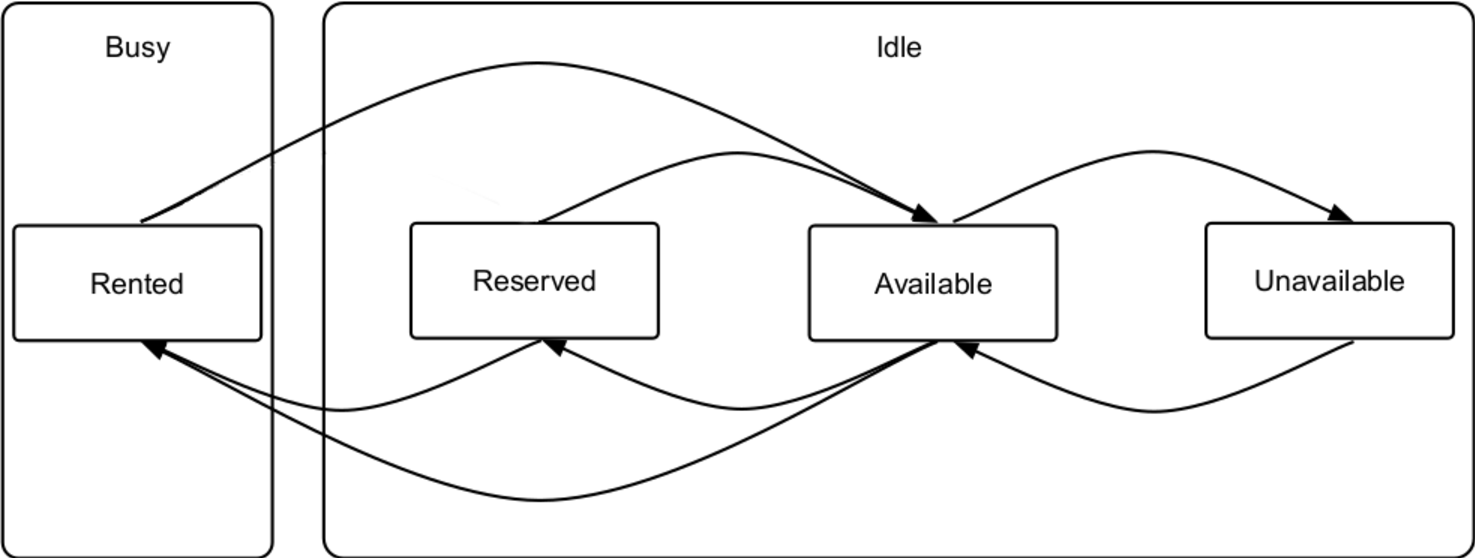
\includegraphics[width=1\textwidth]{imagens/diagrama_v4.pdf}
\caption{Possible states of a vehicle in a car-sharing system.}
\label{fig:diagrama}
\end{figure}

\section{Datasets and crawling methodology} 
\label{sec:3_4_methodology}

%FLEET OF CS systems
Our work relies on usage data from three car-sharing services: Modo, Car2Go, and Evo. These services operate in several cities and countries. We focus on data from the Vancouver area, where all these three services operate. Modo fleet is composed of combustion, electric and hybrid cars; Car2go offers combustion cars and finally, Evo supplies only hybrid vehicles. For each service, we collected both users' trips and fleets composition. In total, we observed more than 680 cars for Modo, 1\,200 for Car2go, and 1\,000 for Evo.

% DATA COLLECTION
For all the three services, we collected vehicle status minute-by-minute, through public Application Programming Interfaces (APIs) or, directing accessing their service information web-page. We can get some values like vehicle ID and position.  In short, through the Modo API\footnote{Modo API, \url{http://modo.coop/api/}} we can obtain the station of a vehicle and the period it is available, reserved or running.
The data we get from Evo\footnote{Evo public portal, \url{https://www.evo.ca/api/Cars.aspx}} information page allow us to check the remaining fuel  (in percentage) of a vehicle and its location. Finally, Car2go APIs\footnote{Car2go API, \url{https://www.car2go.com/api/tou.htm }} output is similar to the Evo's one. 
Data from Evo and Modo comprises five months, ranging from March 1st, 2018 to July 16th, 2018. Car2Go data comprises thirteen months, ranging from  December 31st, 2016 to January 31st, 2018. It is important to notice that, to not violate the users' privacy, the providers do not expose any users' personal information. Moreover, the companies do not track the cars during a trip so we do not know exactly the travel path, but only the start/end positions and the duration of travel.

All measurements used in our analyses are publicly available the following trace repository:
\url{http://netlab.ice.ufjf.br/index.php/carsharingdata/}

%In the following, we further explain each service crawling methodology and the data we use in our analysis.

%In Modo, we infer the reservation period by the availability intervals and the minute-by-minute collect, whereas Evo and Car2Go data allow us to exactly trigger the moments in which the users begin and over their trips, with a precision of one minute, just monitoring the state of all cars. 


\subsection{Modo crawling methodology and data summary}


%%%%%%%%%%%%%%%%%%%%%%%%%%%%%%%%%%%%%%%%%%%%%%%%%%5

%MODO data collection
The Modo data collection process was conducted with a crawler that uses its public API. 
First, we request to the Modo API the list of all vehicles of the service. 
Then, minute by minute, we request the status of each of these vehicles. Each request returns the schedule of a vehicle, informing the periods it will be available for the next 24-hours. Moreover, it returns the vehicle location, i.e., the station with its identifier. 
Note that Modo API does not return specific vehicle status, nor any information that could be used to identify users of the system. We uncover if a vehicle is busy or idle based on its reservation period and the current observation time. In other words, we collect several vehicle schedules and compare each other.
Figure~\ref{fig:capturas} illustrates the process of collecting data for a given vehicle. Each data sample corresponds to a request to the API in the order they occur. Data sample \#1 is the result of the API request at minute 1 ($t=1$), data sample \#2 is the result of the API request at minute 2 ($t=2$), etc. At each data sample, the blue dot represents the time a vehicle will be available. We highlight three possible situations:

\begin{itemize}
\item First, as shown in Figure~\ref{fig:capturas}(a), at $t=1$ a given vehicle is shown reserved up to $t=5$.  At $t=2$, the new request to the Modo API still show us that the vehicle will be available only at $t=5$. Each of the following requests to the API confirms the booking period. At the time $t=6$, we perform a request to the API and the vehicle is no longer booked. In sum, we are able to infer that someone booked the vehicle before or at $t=1$, and returned it to the station at $t=5$.

\item Second, as shown in Figure~\ref{fig:capturas}(b), at $t=1$  the Modo API returns that a given vehicle is reserved up to $t=6$.  However, in this case, a request at $t=5$ shows the vehicle is no longer reserved. In this case, we can infer that the user returned the vehicle earlier to the station which means she/he used the vehicle only up to $t=5$.

\item Finally, as shown in Figure~\ref{fig:capturas}(c), the user may extend the booking period. More precisely, at $t=1$ the given vehicle is reserved up to $t=5$. At the third request, we note that the vehicle will no longer be available at $t=5$ but $t=6$. The following API requests confirm the use of the car until $t=6$.
\end{itemize}


\begin{figure}[!htb]
\centering
    \begin{minipage}[b]{0.25\linewidth}
      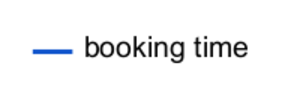
\includegraphics[height=0.8cm]{modo_methodology/time.pdf}
    \end{minipage}\hspace{-5mm}
    \begin{minipage}[b]{0.25\linewidth}
      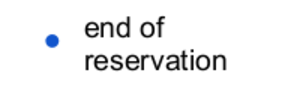
\includegraphics[height=0.8cm]{modo_methodology/point.pdf}
    \end{minipage}

    \medskip
    \begin{minipage}[b]{0.32\linewidth}
    \centering
     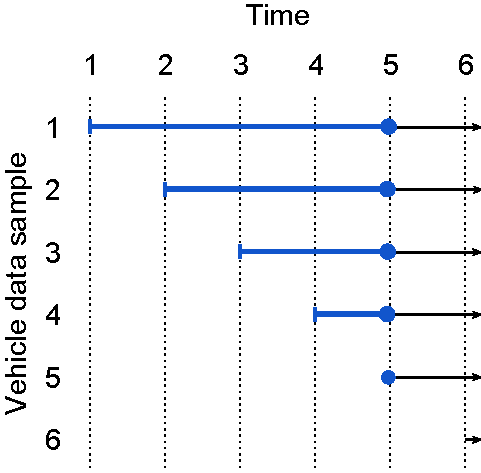
\includegraphics[width=30mm]{modo_methodology/Normal_Situation.pdf}
     {\\(a) Normal \\situation}
    \end{minipage}
    % \hspace{5mm}
    \begin{minipage}[b]{0.32\linewidth}
     \centering
     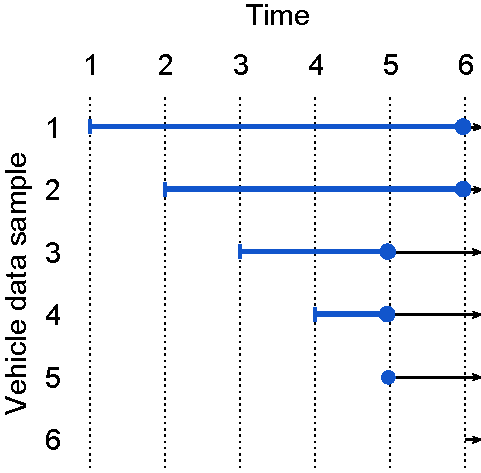
\includegraphics[width=30mm]{modo_methodology/Cancelation_Situation.pdf}
    %  \vspace*{-3mm}
     {\\(b) Anticipated vehicle return}
    \end{minipage}
    %\hspace{1cm}
    %\hspace{5mm}
    \begin{minipage}[b]{0.32\linewidth}
    % \vspace{5mm}
     \centering
     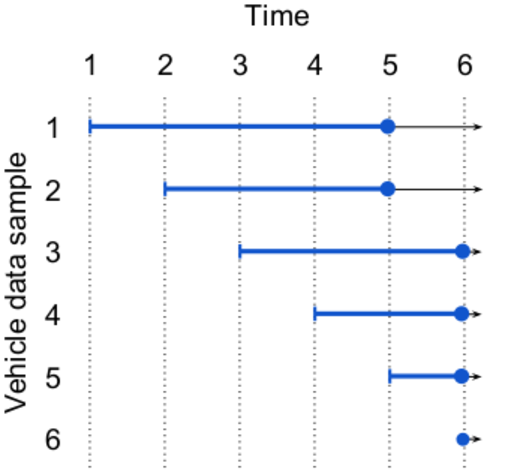
\includegraphics[width=30mm]{modo_methodology/Consecutive_without_legend.pdf}
     {\\(c) Extended travel situation}
    \end{minipage}
    \caption{Possible vehicle status during the Modo crawling. In (a) a normal booking and usage situation; (b) a cancellation situation; (c) a consecutive booking situation.}
    \label{fig:capturas}
\end{figure}

Besides, we also collect base stations location, vehicle models and whether the vehicle is electric or hybrid. 
Table~\ref{table:dataModo} summarizes the data we have collected from Modo. We stored 134 millions of records in 5 months, from a fleet of 682 vehicles distributed in 528 stations, each of them with one or more cars. The stations are located in Vancouver, Canada, and its neighbor cities. This data allows us to analyze more than %149 thousands of booking records and 
98\,000 travels.\footnote{Data are available on http://netlab.ice.ufjf.br/index.php/carsharingdata/}
% \footnote{Data will be available for researchers upon request.}

\begin{table}[tbh]
\centering
\scriptsize
\begin{tabular}{llr}
%\multicolumn{2}{l}{Description}                     & Amount \\ 
\hline
\multicolumn{2}{l}{\# of Collected Records}  & $\approx$ 134\,000\,000\\
\multicolumn{2}{l}{\# of Booking Records} & 149\,732  \\
\multicolumn{2}{l}{\# of Travels Records} & 98\,915   \\
\multicolumn{2}{l}{\# of Stations} & 528    \\\hline   
\multirow{3}{*}{\# of Vehicles}       & - Common    & 530 \\
                                      & - Hybrids  & 148 \\
                                      & - Electrical & 4 \\
                                      \hline
\end{tabular}
\caption{Summary of the Modo dataset.}
\label{table:dataModo}
\end{table}


%%%%%%%%%%%%%%%%%%%%%%%%%%%%%%%%%%%%%%%%%%%%%%%

\subsection{Evo crawling methodology and data summary}

Evo does not offer a public API to researchers. For this reason, we collect data which is publicly available at its web portal. Minute by minute, we retrieve a list of all system vehicles. Moreover, we request service snapshots, describing which vehicles are parked, where they are parked and if they are available to travel. 
We process all snapshots of the system to infer the moments a vehicle is busy (rented) or idle (parked at a station). During a snapshot, if a vehicle is listed among the system vehicles but it is not parked at any station, we infer it is in use. Then, we set-up the travel starting point as the last station the vehicle was parked. Analogously, the travel ending point will be the next station the vehicle appears in a future snapshot. The total travel time is accounted for as the difference between these snapshots times. 
For each travel we identify, we also record the end-to-end path, according to the Google Maps API. In this way, we are also able to calculate the estimated travel, taking into account the local traffic conditions. Clearly, this estimation does not take into account the car-sharing client behavior and, as a consequence, differ from the real travel time we also store. 
One may reserve a car in Evo and cancel this reservation, within a thirty minutes range, without any charges. Thus, we infer the number of cancellation in Evo by filtering short travels (i.e., $<$ 30 minutes) where the start and end points are the same. To accommodate GPS imprecision, we consider a 3~meters threshold. 
Table~\ref{table:dataEvo} summarizes the data we collect from Evo.
%In short, we collected more than 10 million records and 1 million travels, of a fleet with more than a one thousand vehicles and 130 stations. 
Note that this service does not need a large number of stations because the user can park the car in some public park spots in the service area, that is called home zone (Vancouver and its neighbor cities).

\begin{table}[htb]
\centering
\scriptsize

\begin{tabular}{llr}
%\multicolumn{2}{l}{Description} & Amount\\ 
\hline
\multicolumn{2}{l}{\# of Collected Records} & 142\,853\,500
\\
\multicolumn{2}{l}{\# of Travels Records} &  644\,887\\
%1\,232\,262\\
\multicolumn{2}{l}{\# of Stations}  & 130  \\\hline
\multicolumn{2}{l}{\# of Vehicles} & 1\,237
%1\,003 
\\\hline
\end{tabular}
\caption{Summary of the Evo data collection.}
\label{table:dataEvo}
\end{table}

\subsection{Car2Go crawling methodology and data summary}

Car2Go offers APIs providing information about available cars at the moment of the request. Each API request returns, among other information, the car unique ID, its position and other fields which specifically describe the car status. Therefore the API response is semantically equivalent to the Evo's one. In this way, we applied the same methodology to gather and store the Car2go data too.

There are two main events, which changes the car status, clearly observable from the data. Considering the current time instant $t_i$: 
\begin{itemize}
     \item if in $t_i$ the car is present in the API response and at time $t_{i+1}$ it is not, that car passes from available to rented. %It represents a parking event finish and a booking.
     \item if in $t_i$ the car is \emph{not} present and at time $t_{i+1}$ it reappears in the API reply, that car passes from rented  to available. It represents a booking finish and a parking beginning.  Indeed, for privacy constraints, the position of the car during a booking is not available.
\end{itemize}

Notice that from a single rented status is impossible to estimate the traveled distance: by computing the Euclidean or Haversine 
distance we obtain only a lower bound of the real travel distance which is practically too optimistic to be used as a primary travel estimation. To improve this estimation we attach to each entry the distance provided by the Google Maps API. 
As in Evo's methodology, we infer the number of cancellations by filtering short travels where the start and end points are very close. Table~\ref{table:dataCar2Go} summarizes Car2go dataset. We have more than one million travels in our thirteen months of data. As a free-floating service, Car2Go does not have stations but it has an operation zone, that covers a large area of Vancouver city and North-Vancouver. 

\begin{table}[htb]
\centering
\scriptsize
\begin{tabular}{llr}
%\multicolumn{2}{l}{Description} & Amount\\ 
\hline
\multicolumn{2}{l}{\# of Travels Records} & 1\,095\,577\\
%1\,340\,053\\
\multicolumn{2}{l}{\# of Vehicles} & 1\,077
%1\.273 
\\\hline
\end{tabular}
\caption{Summary of the Car2Go data collection.}
\label{table:dataCar2Go}
\end{table}

\section{Car-sharing services characterization} 
\label{sec:4_4_characterization}

In this section, we first present temporal characterization of the three services (Section~\ref{sec:temporal_characterization}). Then, we describe the services spatial-temporal characteristics (Section~\ref{sec:spatial-temporal}). Finally, we present users' behavior (Section~\ref{sec:user-behavior}).

\subsection{Temporal characteristics}\label{sec:temporal_characterization}


\begin{figure}
	\centering
	\subfloat[\centering Two-way Modo Weekdays]{{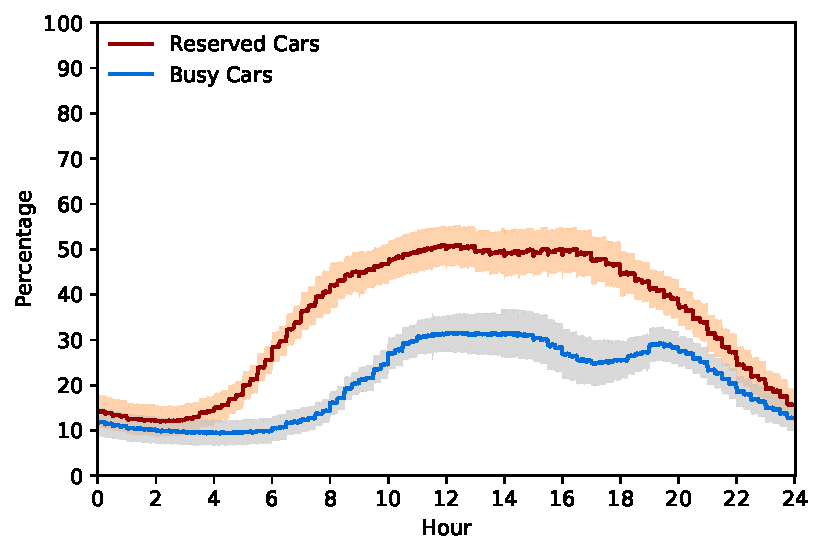
\includegraphics[width=0.46\columnwidth]{modo_inTravel/weekdays.pdf}} \label{fig:modo_wd}}%
	\qquad
	\subfloat[\centering Two-way Modo Weekends]{{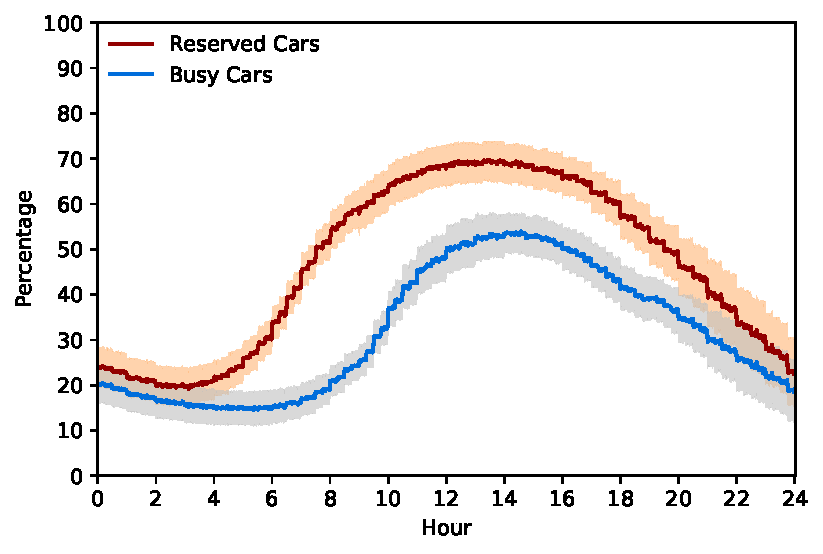
\includegraphics[width=0.46\columnwidth]{modo_inTravel/weekends.pdf}} \label{fig:modo_we}}%
	\caption{Modo Minute-by-minute mean value (plus/minus standard deviation) for  the  percentage of busy (blue curve) and reserved cars (red curve), for weekdays and weekends}
	\label{fig:4_4_modo_busy}%
\end{figure}


\begin{figure}
	\centering
	\subfloat[\centering One-way Evo Weekdays]{{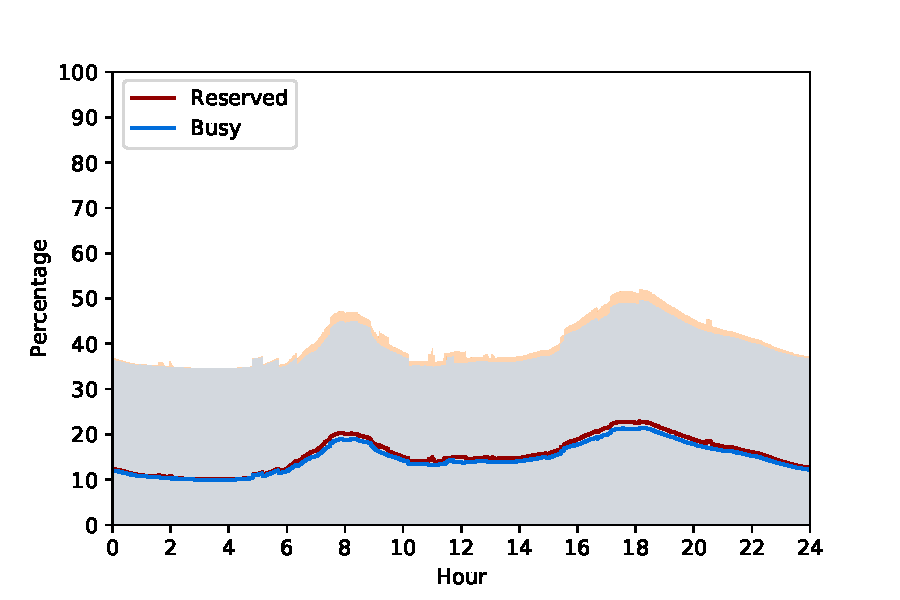
\includegraphics[width=0.46\columnwidth]{evo_inTravel/weekdayslim.pdf}} \label{fig:evo_wd}}%
	\qquad
	\subfloat[\centering One-way Evo Weekends]{{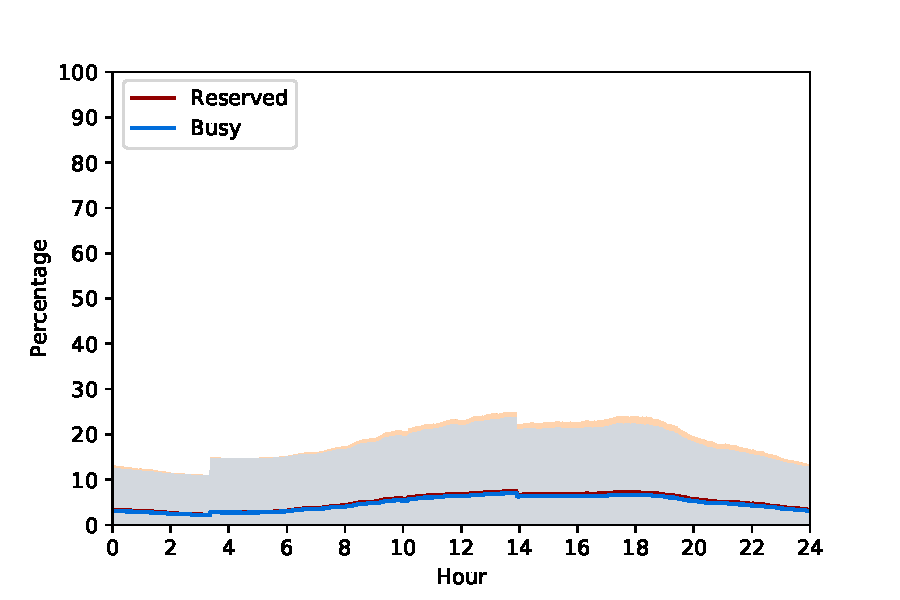
\includegraphics[width=0.46\columnwidth]{evo_inTravel/weekendslim.pdf}} \label{fig:evo_we}}%
	\caption{Evo Minute-by-minute mean value (plus/minus standard deviation) for  the  percentage of busy (blue curve) and reserved cars (red curve), for weekdays and weekends}
	\label{fig:4_4_evo_busy}%
\end{figure}

\begin{figure}
	\centering
	\subfloat[\centering Free floating car2Go Weekdays]{{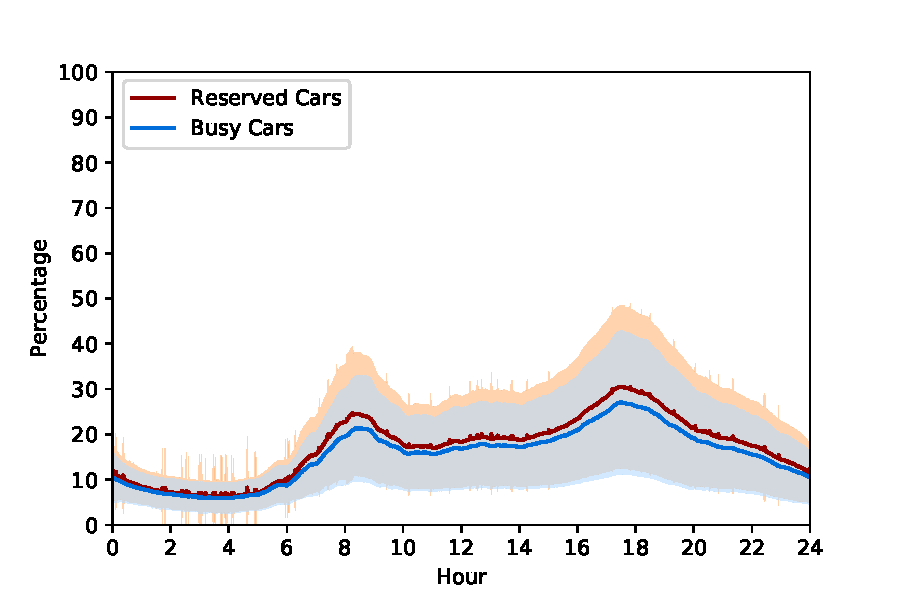
\includegraphics[width=0.46\columnwidth]{car2go_inTravel/weekdayslim.pdf}} \label{fig:c2g_wd}}%
	\qquad
	\subfloat[\centering Free floating car2Go Weekends]{{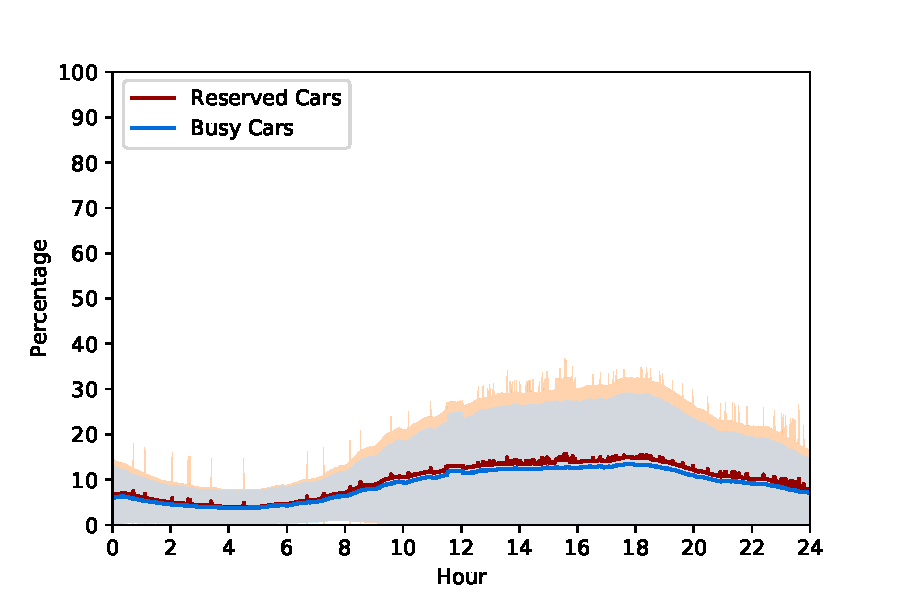
\includegraphics[width=0.46\columnwidth]{car2go_inTravel/weekendslim.pdf}} \label{fig:c2g_we}}%
	\caption{car2go Minute-by-minute mean value (plus/minus standard deviation) for  the  percentage of busy (blue curve) and reserved cars (red curve), for weekdays and weekends}
	\label{fig:4_4_c2g_busy}%
\end{figure}

%PRENSENTATION OF FIGURE
Figures~\ref{fig:4_4_modo_busy}, \ref{fig:4_4_evo_busy} and \ref{fig:4_4_c2g_busy} show the service daily demand pattern. In all plots, the blue and red solid lines refer to a minute-by-minute mean value over the studied period for the percentage of busy and reserved cars, respectively, for each service. The plots show also the standard deviation from the mean as the smoothed gray and orange background areas around the mean. On the left of each pair of figures (figures \ref{fig:modo_wd}, \ref{fig:evo_wd} and \ref{fig:c2g_wd}) is presented the demand pattern during working days, while on the (figures \ref{fig:modo_we}, \ref{fig:evo_we} and \ref{fig:c2g_we}) is shown the demand for weekends (Saturdays, Sundays, and festivities). 

%Overall, this figure highlights four main insights about the daily demand for the three services: (i) all of them present differences between weekdays and weekends; (ii) Modo has a distinct demand pattern when compared to the other two services; (iii) the number of cancellations is considerable in Modo and; (iv) the variation on demand, considering all analyzed period is small for Modo, but it is large for Evo and Car2go.

%DESCRIPTION OF INSIGHTS OF FIGURE
All three services present two peaks of demand during weekdays and only one during the weekends. During weekdays, for Evo and Car2Go, the one-way and free-floating services, the peaks of demand occur about 8~AM and 6~PM whereas for Modo, the two-way service, these peaks occur around 2~PM and 7~PM.
Moreover, note that for Evo and Car2Go, weekdays demand is higher than during weekends. On the other hand, for Modo, we observe just the opposite. 
Mostly, Modo users are regulars and present weekly/daily/hourly subscription. In this sense, they tend to reserve cars at the same hour, for regular periods, which explains Modo lower variation. For a given moment, we consider the relative difference between the reserved and busy cars as the cancellations of the system. Modo presents up to 60\% of cancellations, while the other two services present no more than 5\%. 
%For Modo, during weekdays, the cancellations often occur during all the day, including on the peak hours. During weekends, on the other hand, the number of cancellations is lower in the Modo peak of use. \lv{Not completely true from the plot}



\begin{figure}[htb]
\centering
    \begin{minipage}[b]{0.45\linewidth}
    \centering
     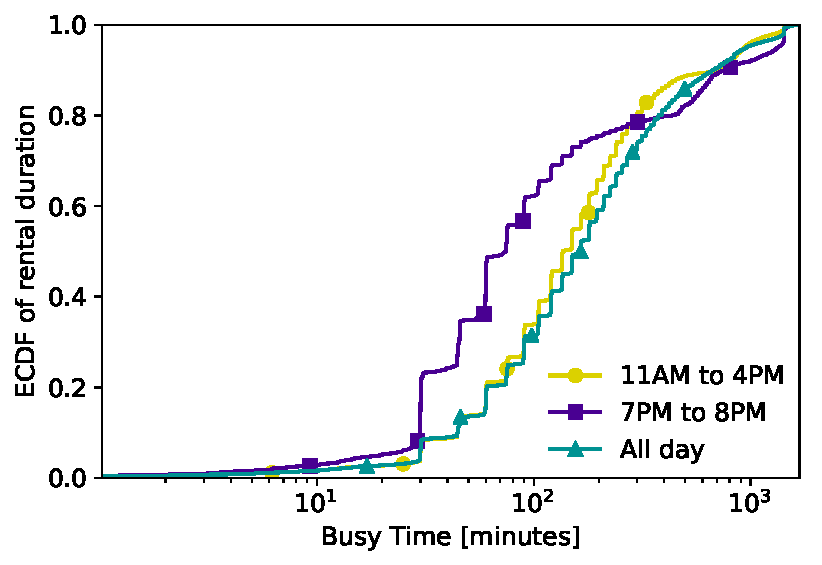
\includegraphics[width=59mm]{modo_cdfs/modo_tarde_noiteCDF_rebuttal.pdf}
     {\\(a) Two-way Modo}
    \end{minipage}
    \hspace{5mm}
    \begin{minipage}[b]{0.45\linewidth}
     \centering
     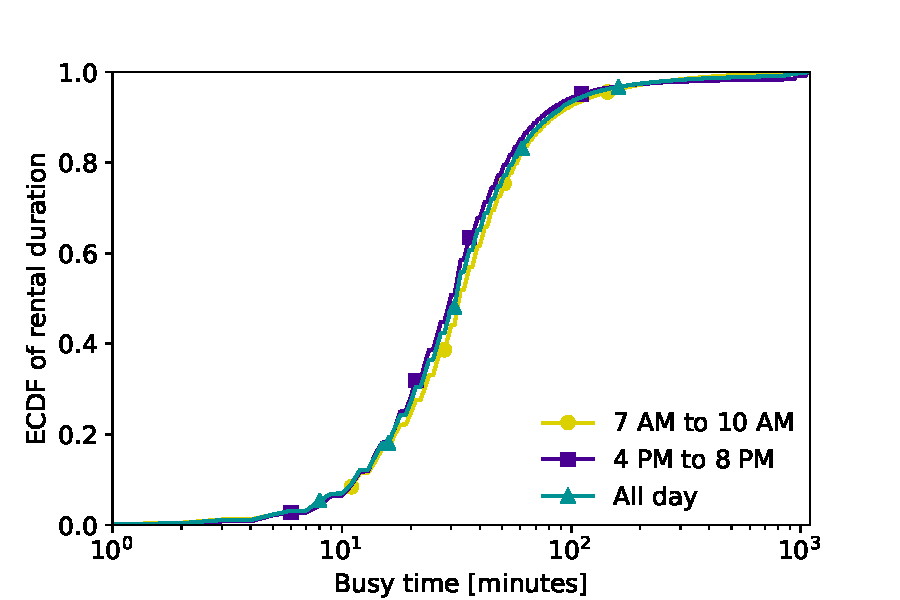
\includegraphics[width=65mm]{evo_cdfs/evo_tarde_noiteCDF_rebuttal.pdf}
     \vspace*{-3mm}
     {\\(b) One-way Evo}
    \end{minipage}
    %\hspace{1cm}
    %\hspace{5mm}
    \begin{minipage}[b]{0.45\linewidth}
    \vspace{5mm}
     \centering
     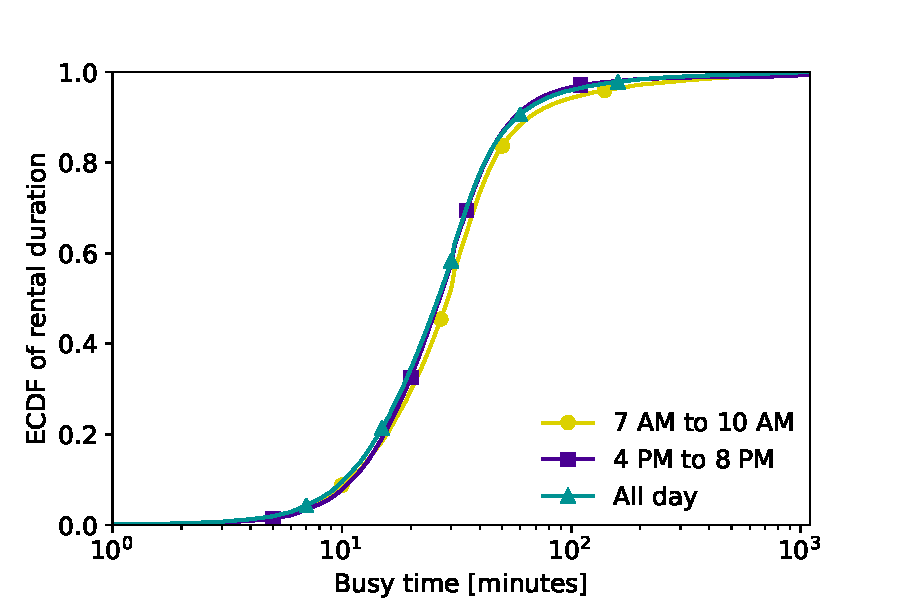
\includegraphics[width=65mm]{car2go_cdfs/c2g_tarde_noiteCDF_rebuttal.pdf}
     {\\(c) Free floating Car2Go}
    \end{minipage}
    \caption{Cumulative distribution function of vehicle busy time during a weekday.}
    \label{fig:cdfs_picos}
\end{figure}

%DESCRIPTION OF FIGURE
Figure~\ref{fig:cdfs_picos} presents the Empirical Cumulative Distribution Function (ECDF) of vehicles busy time, i.e., the rental duration, during load peaks of the day. In this case, we evaluate the load periods from 7~AM to 10~AM and from 4~PM to 8~PM for free-floating and one-way, from 11~AM to 4~PM and 7~PM to 8~PM for two-way, and also all-day data for the three services. 

%INSIGHTS OF FIGURE
As for the demand, Evo and Car2Go present similar behaviour, which is different from Modo. For Modo it is possible to observe at least 80\% of vehicles rentals presents more than 1 hour of occupation, with more than 10\% of rentals that last for more than 15 hours. On the other hand, Evo and Car2Go usually present shorter rentals, with no more than 10\% of vehicles busy for more than one hour. 
In sum, the most notable differences between these services occur due to their business model. Indeed, Modo presents a strict policy, where users must pick-up a car and leave it at the same station. However, Modo presents a flexible policy regarding cancellations. The other two services, only allow users to cancel the rent of a vehicle up to 30 minutes after its booking.


%%%%%%%%%%%%%%%%%%%%%%%%%%%%%%%%%%%%%%%%
\subsection{Spatial-temporal characteristics}
\label{sec:spatial-temporal}


%modo
\begin{figure}[hhh!!]
\centering
   \begin{minipage}[b]{0.3\linewidth}
   \centering      
         \begin{minipage}[b]{\linewidth}
           \hspace*{-0.9cm}
           \centering
           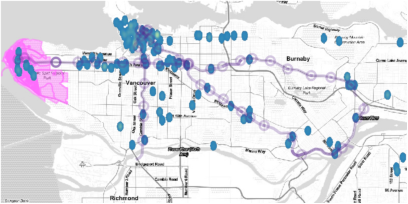
\includegraphics[width=42mm]{modo_heatmaps/min/0.pdf}
           {\\(a) 0~AM to 1~AM}
         \end{minipage}
         %\hspace{3mm}
         \begin{minipage}[b]{\linewidth}
           \centering
           \hspace*{-0.9cm}
           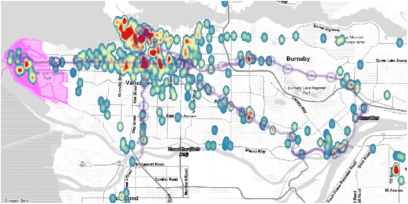
\includegraphics[width=42mm]{modo_heatmaps/min/8.pdf}
           {\\(c) 8~AM to 9~AM}
         \end{minipage}
         \begin{minipage}[b]{\linewidth}
           \centering
           \hspace*{-0.9cm}
           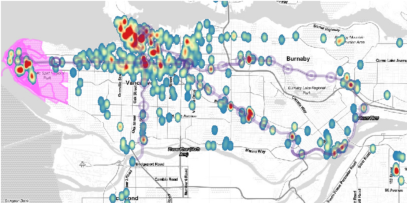
\includegraphics[width=42mm]{modo_heatmaps/min/16.pdf}
           {\\(e) 4~PM to 5~PM}
         \end{minipage}
   \end{minipage}
   \hspace{3mm}
   \begin{minipage}[b]{0.3\linewidth}
   \centering
         \begin{minipage}[b]{\linewidth}
           \centering
           \hspace*{-0.1cm}
           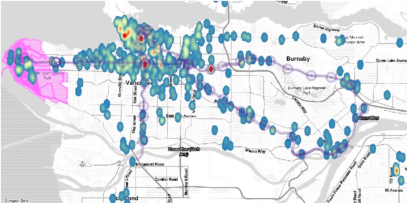
\includegraphics[width=42mm]{modo_heatmaps/min/4.pdf}
           {\\(b) 4~AM to 5~AM}
         \end{minipage}
         %\hspace{3mm}
         \begin{minipage}[b]{\linewidth}
           \centering
           \hspace*{-0.1cm}
           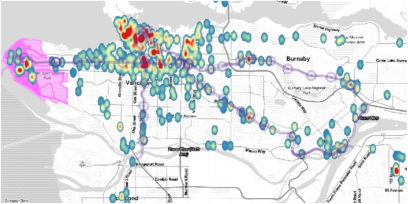
\includegraphics[width=42mm]{modo_heatmaps/min/12.pdf}
           {\\(d) 12~AM to 1~PM}
         \end{minipage}
         \begin{minipage}[b]{\linewidth}
           \hspace*{-0.1cm}
           \centering
           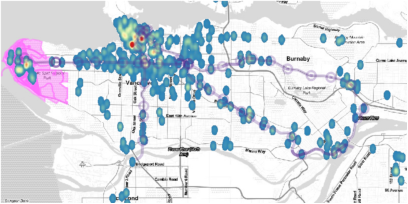
\includegraphics[width=42mm]{modo_heatmaps/min/20.pdf}
           {\\(f) 8~PM to 9~PM}
         \end{minipage}
   \end{minipage}
   \begin{minipage}[b]{0.1\linewidth}
   \centering
   		 \hspace*{12mm}
   		 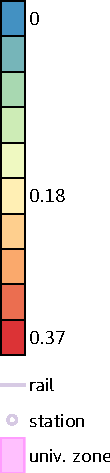
\includegraphics[width=12mm]{modo_heatmaps/legenda_modo.pdf}
         \vspace{17mm}
   \end{minipage}
   %\hspace{1cm}
   \caption{Spatial-temporal service demand for two-way service Modo.}
   \label{fig:heat_modo}
\end{figure}

%evo
% Não é o definitivo
\begin{figure}[hhh!!]
\centering
   \begin{minipage}[b]{0.3\linewidth}
   \centering      
         \begin{minipage}[b]{\linewidth}
           \hspace*{-0.9cm}
           \centering
           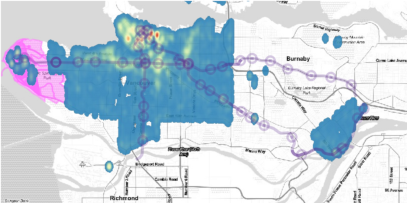
\includegraphics[width=42mm]{evo_heatmaps/min/hora0.pdf}
           {\\(a) 0~AM to 1~AM}
         \end{minipage}
         %\hspace{3mm}
         \begin{minipage}[b]{\linewidth}
           \centering
           \hspace*{-0.9cm}
           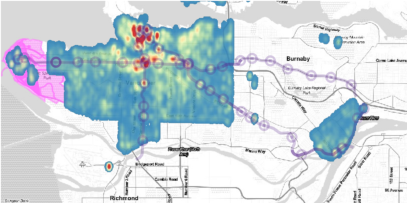
\includegraphics[width=42mm]{evo_heatmaps/min/hora8.pdf}
           {\\(c) 8~AM to 9~AM}
         \end{minipage}
         \begin{minipage}[b]{\linewidth}
           \centering
           \hspace*{-0.9cm}
           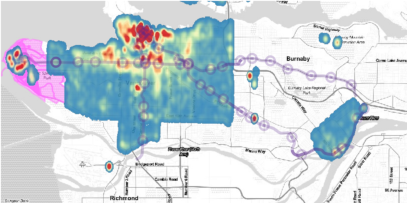
\includegraphics[width=42mm]{evo_heatmaps/min/hora16.pdf}
           {\\(e) 4~PM to 5~PM}
         \end{minipage}
   \end{minipage}
   \hspace{3mm}
   \begin{minipage}[b]{0.3\linewidth}
   \centering
         \begin{minipage}[b]{\linewidth}
           \centering
           \hspace*{-0.1cm}
           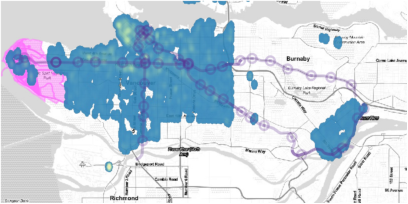
\includegraphics[width=42mm]{evo_heatmaps/min/hora4.pdf}
           {\\(b) 4~AM to 5~AM}
         \end{minipage}
         %\hspace{3mm}
         \begin{minipage}[b]{\linewidth}
           \centering
           \hspace*{-0.1cm}
           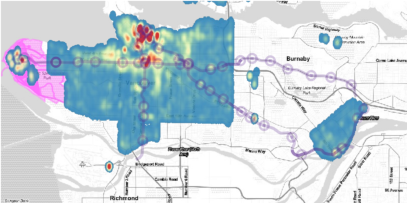
\includegraphics[width=42mm]{evo_heatmaps/min/hora12.pdf}
           {\\(d) 12~AM to 1~PM}
         \end{minipage}
         \begin{minipage}[b]{\linewidth}
           \hspace*{-0.1cm}
           \centering
           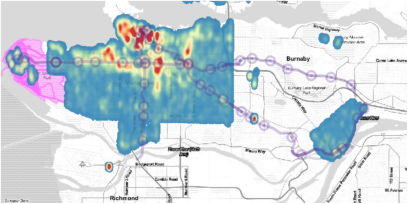
\includegraphics[width=42mm]{evo_heatmaps/min/hora20.pdf}
           {\\(f) 8~PM to 9~PM}
         \end{minipage}
   \end{minipage}
   \begin{minipage}[b]{0.1\linewidth}
   \centering
   		 \hspace*{12mm}
   		 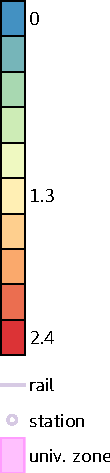
\includegraphics[width=12mm]{evo_heatmaps/legenda_evo.pdf}
         \vspace{17mm}
   \end{minipage}
   %\hspace{1cm}
   \caption{Spatial-temporal service demand for one-way service Evo.}
   \label{fig:heat_evo}
\end{figure}

% car2go
\begin{figure}[hhh!!]
\centering
   \begin{minipage}[b]{0.3\linewidth}
   \centering      
         \begin{minipage}[b]{\linewidth}
           \hspace*{-0.9cm}
           \centering
           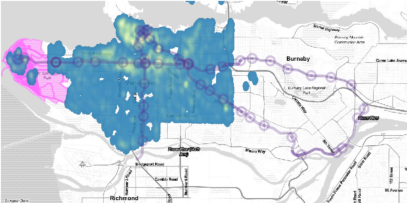
\includegraphics[width=42mm]{car2go_heatmaps/min/0.pdf}
           {\\(a) 0~AM to 1~AM}
         \end{minipage}
         %\hspace{3mm}
         \begin{minipage}[b]{\linewidth}
           \centering
           \hspace*{-0.9cm}
           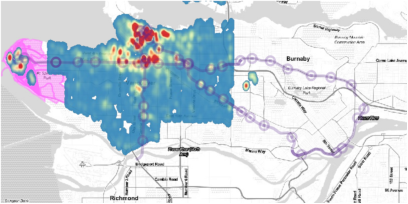
\includegraphics[width=42mm]{car2go_heatmaps/min/8.pdf}
           {\\(c) 8~AM to 9~AM}
         \end{minipage}
         \begin{minipage}[b]{\linewidth}
           \centering
           \hspace*{-0.9cm}
           \includegraphics[width=42mm]{car2go_heatmaps/min/16.pdf}
           {\\(e) 4~PM to 5~PM}
         \end{minipage}
   \end{minipage}
   \hspace{3mm}
   \begin{minipage}[b]{0.3\linewidth}
   \centering
         \begin{minipage}[b]{\linewidth}
           \centering
           \hspace*{-0.1cm}
           \includegraphics[width=42mm]{car2go_heatmaps/min/4.pdf}
           {\\(b) 4~AM to 5~AM}
         \end{minipage}
         %\hspace{3mm}
         \begin{minipage}[b]{\linewidth}
           \centering
           \hspace*{-0.1cm}
           \includegraphics[width=42mm]{car2go_heatmaps/min/12.pdf}
           {\\(d) 12~AM to 1~PM}
         \end{minipage}
         \begin{minipage}[b]{\linewidth}
           \hspace*{-0.1cm}
           \centering
           \includegraphics[width=42mm]{car2go_heatmaps/min/20.pdf}
           {\\(f) 8~PM to 9~PM}
         \end{minipage}
   \end{minipage}
   \begin{minipage}[b]{0.1\linewidth}
   \centering
   		 \hspace*{12mm}
   		 \includegraphics[width=12mm]{car2go_heatmaps/legenda_car2go.pdf}
         \vspace{17mm}
   \end{minipage}
   %\hspace{1cm}
   \caption{Spatial-temporal service demand for free-floating service Car2Go.}
   \label{fig:heat_car2go}
\end{figure}

Figures~\ref{fig:heat_modo}, \ref{fig:heat_evo} and \ref{fig:heat_car2go} present heat-maps of the hourly\footnote{Due to space constraints, we only show one-hour period every four hour.} mean number of busy vehicles in a given location, considering analyzed period. In the case of Modo, a location refers to a fixed station. In the case of the other two services, the maps present clustered travel records where users pick-up or leave a vehicle. To cluster these points the algorithm uses a 400\,m radius as a reference, forming a region close to a neighborhood. Rangin radius from 100\,m to 1000\,m, leads to similar results. 

First, all three services present a large demand in the downtown area and the university zone. Note that the demand in downtown for all three services is low during the night, starts increasing at 4-5 AM, reaches its peak during office working hours and reduces by the end of the day. In this case, users usually pick-up cars to their daily tasks, as go to work and shopping. During the night, usage increases in the surroundings of the city, the university zone, and neighborhoods with leisure facilities (such as bars). 
Modo presents a distinct demand pattern. Indeed, Modo has fixed stations located along with the existing public transport system, especially the Expo Line and Millennium Line. For this reason, it is possible to highlight a strong relationship between the existing public transport system and the car-sharing system demand. On the other hand, the other two services are more flexible. Users can rent a car almost anywhere. In this sense, despite the major demand in downtown, it is present a widespread demand all over the city.

Figures~\ref{fig:matrixEvo} and \ref{fig:matrixCar2Go} detail the spatial-temporal demand for Evo and Car2Go by presenting their origin-destination matrix mapped on 31 city areas as defined by the metropolitan city of Vancouver. To enhance the visual effects, we normalized the previous heat-maps values to a scale between 0-1, using the min-max method. Moreover, due to space constraint, this work shows the origin-destination matrix at a specific hour, i.e., at 4\,PM.
In general, the users tend to start and end a trip at the same location. It appears that during working days, users tend to use a shared car  returning it to the same region where they start (likely where they are working or living). However, for both services, a non-negligible probability to spread services along all city area is noticeable. 
Moreover, we also note that some regions serve as hubs. This is more notable for Evo service. As shown in Figure~\ref{fig:matrixEvo}, the downtown area serves as a hub to start trips to almost all other regions. The opposite (a high tendency to start a trip ending at downtown) trend is not present. As a consequence, service may become unbalanced and, from time to time, service maintenance should relocate vehicles from a region to another, to accommodate the daily demand.

\begin{figure}[tbh]
\centering
\includegraphics[width=0.85\columnwidth]{destination_matrix/hour16.png}
\caption{Origin-destination matrix for one-way service Evo (from 4~PM to 5~PM).}
\label{fig:matrixEvo}
\end{figure}
%
\begin{figure}[tbh]
\centering
\includegraphics[width=0.85\columnwidth]{car2go_destination_matrix/hour16.png}
\caption{Origin-destination matrix for free-floating service Car2Go (from 4~PM to 5~PM).}
\label{fig:matrixCar2Go}
\end{figure}


%%%%%%%%%%%%%%%%%%%%%%%%%%%%%%%%%%%


\subsection{User behavior characteristics}
\label{sec:user-behavior}


Vehicles busy and idle periods direct impacts service revenue. Indeed, the longer the busy period is and the lower the idle period of a vehicle is, the more profitable the car will be. Therefore, the work characterizes the busy and idle periods of vehicles for all three services. In this analysis, are considered all the vehicles and all the trips lasting less than 90 minutes, which corresponds to more than 99.5\% records. 
For each service, we identified the statistical distribution that best fits the actual data (busy and idle period). For this purpose, we tested more than 40 well-known statistical distributions. More in-depth, for each component of the model, the parameters of the distribution that most closely approximate the data are determined using the Maximum Likelihood Estimation (MLE) method. After defining the parameters of each component of the model, the ten distributions with shorter Kolmogorov-Smirnov distance (continuous distributions) or lower least square error (discrete distributions) concerning the data are chosen. Finally, we chose the top three common distributions to each car-sharing service. These choices are also validated with a visual assessment of the curve fitting.

Figure~\ref{fig:busy_all_eCDF} shows the Cumulative Distribution Function of vehicle busy time.  Modo, Evo and Car2Go busy time and their best statistical distribution fitting are shown in blue, red and yellow, respectively. For all three services, the Inverse~Gamma\footnote{Cumulative distribution function (CDF) of the Inverse~Gamma distribution: $F(x, a, \beta, \delta) = \frac{1}{\Gamma(a)}\int_{1/\left((x-\beta)/\delta\right)}^{\infty}t^{a-1}e^{-t}dt$}, 
the Burr\footnote{Cumulative distribution function (CDF) of the Burr distribution: $F(x,c,d,\beta,\delta)=\left(1 + \left((x-\beta)/\delta\right)^{-c}\right)^{-d}$}, 
and Mielke's Beta-Kappa\footnote{Cumulative distribution function (CDF) of the Mielke's Beta-Kappa distribution: $F(x,k,s,\beta,\delta) = \frac{\left((x-\beta)/\delta\right)^{k}}{(1+\left((x-\beta)/\delta\right)^{s})^{(k*\frac{1}{s})}}$} 
distributions present a  good fitting to the empirical data, with similar MLEs.  
Table~\ref{table:fit_busy} summarizes the parameters of the distributions of the busy time for each statistical distribution.
Despite all three services present the same statistical distribution fitting, 
the two-way service (i.e., Modo), presents a clear shift to right on its curve when compared to the other two services, as shown in Figure~\ref{fig:busy_all_eCDF}. As we previously discussed, the median busy time on Modo is more than one hour longer than the median busy time for the other services. 
Users in Modo must return cars to the same station they originated travels. As a consequence, they tend to perform longer tasks. On the other hand, with the other two services users tend to do a longer number of shorter travels.

Finally, Figure~\ref{fig:idle_all_eCDF}, presents vehicle idle periods distribution.  Power~log~normal\footnote{Cumulative distribution function (CDF) of the Power~log~normal distribution: $F(x,c,s,\beta,\delta)=1-\left(\frac{1}{\sqrt{2\pi}}\int_{-\infty}^{-log((x-\beta)/\delta)/s}e^{-t^{2}/2}dt\right)^{c}$}, Burr and Mielke's~Beta$-$Kappa distributions best fit the idle data, for all three datasets. Table~\ref{table:fit_idle} presents the distribution parameters. 
Again, Modo presents a distinct behavior from the other two services. The longer idle period for Modo vehicles corroborates to our previous observations. Indeed, the demand for car-sharing varies over the city during a day. While users in Evo and Car2Go can park anywhere, they contribute to spreading cars over the city. For example, at least 75\% of cars in Modo remains idle for periods longer than 2 hours. For the other two services, no more than 20\% of vehicles remains idle for the same period.

In sum, our analysis shows that the free-floating and one-way car-sharing systems have similar characteristics. They are mostly used for short/medium period travels, while the two-way system is mostly used for medium to long travels. 
Moreover, Evo and Car2Go dynamically spread car over the city, turning the car's idle periods shorter. The longer number of shorter travels, associated with the shorter idle periods, may indicate a more profitable service.

\begin{figure}[tbh]
   \centering
   \includegraphics[width=0.85\columnwidth]{images_test/CDF_Fit_final.pdf}
   \caption{Cumulative distribution function of vehicle busy time.}
   \label{fig:busy_all_eCDF}
\end{figure}


\begin{table}
\centering
\setlength{\tabcolsep}{2.3pt}
	\begin{tabular}{lll}
	\hline
	\multirow{3}{*}{Modo}   & Inv.Gamma       & a = 1.7032,  $\beta$ = -38.5120,  $\delta$ = 278.8487                        \\
	                        & Burr                & c = 1.5651, d = 1.0327,  $\beta$ = -1.8893, $\delta$ = 163.0525 \\
	                        & Mielke & k = 1.59745, s = 1.5687,  $\beta$ = -1.6713, $\delta$ = 164.9877 \\ \hline
	\multirow{3}{*}{Evo}    & Inv.Gamma       & a = 2.0674, $\beta$ = -4.7928, $\delta$ = 63.4382                          \\
	                        & Burr                & c = 1.8332, d = 1.5078, $\beta$ = -0.1855, $\delta$ = 23.5794   \\
	                        & Mielke & k = 2.7305, s = 1.8336, $\beta$ = -0.1125, $\delta$ = 23.7291 \\ \hline
	\multirow{3}{*}{Car2Go} & Inv.Gamma       & a = 2.7688, $\beta$ = -4.9702, $\delta$ = 75.2494                           \\
	                        & Burr                & c = 2.3869, d = 64.2072, $\beta$ = -12.5240, $\delta$ = 5.7419   \\
	                        & Mielke & k = 37.8163, s = 2.3450, $\beta$ = -10.9187, $\delta$ = 9.6407   \\ \hline
	\end{tabular}
\caption{Distributions parameters of the busy time fit curves. The $\beta$ and $\delta$ are key parameters to adjust the location and scale of the distributions.}
\label{table:fit_busy}
\end{table}

\begin{figure}
   \centering
   \includegraphics[width=0.85\columnwidth]{images_test/CDF_Fit_idle_final.pdf}
   \caption{Cumulative distribution function of vehicle idle time}
   \label{fig:idle_all_eCDF}
\end{figure}


\begin{table}
\centering
\setlength{\tabcolsep}{2.3pt}
	\begin{tabular}{lll}
	\hline
	\multirow{3}{*}{Modo}   & PLogNorm       & c = 118.7142, s=3.6088,  $\beta$=0.7191,  $\delta$=3780209.5149                     \\
	                        & Burr                & c = 1.9865, d = 0.3860,  $\beta$ = -7.7229, $\delta$ = 1105.5853 \\
	                        & Mielke & k = 0.8898, s = 1.5390,  $\beta$ = -1.4862, $\delta$ = 860.6790 \\ \hline
	\multirow{3}{*}{Evo}    & PLogNorm       & c = 0.0723, s = 0.7003,  $\beta$ = -0.6723,  $\delta$ = 1.8246                          \\
	                        & Burr                & c = 0.6931, d = 3.7574, $\beta$ = -0.4881, $\delta$ = 2.3713   \\
	                        & Mielke & k = 2.7161, s = 0.5882, $\beta$ = -0.2800, $\delta$ = 0.9725 \\ \hline
	\multirow{3}{*}{Car2Go} & PLogNorm       & c = 4.8747, s = 3.3741,  $\beta$ = 0.7134,  $\delta$ = 1334.7243                           \\
	                        & Burr                & c = 0.7714, d = 0.7337, $\beta$ = 0.7166, $\delta$ = 53.9727   \\
	                        & Mielke & k = 0.5743, s = 0.8826, $\beta$ = 0.7166, $\delta$ = 68.1029   \\ \hline
	\end{tabular}
\caption{Distributions parameters of the idle time fit curves. The $\beta$ and $\delta$ are keyword parameters to adjust the location and scale of the distributions.}	\label{table:fit_idle}

\end{table}



\section{Conclusions} 
\label{sec:3_6_conclusion}

In this article, we characterized three distinct car-sharing systems which operate in  Vancouver  (Canada)  and nearby regions. Our study, using data of more than one year of real trips, uncovers patterns of users’ habits.  We provided a characterization of the different car-sharing services, including spatial-temporal usage. Finally, we highlighted the main differences and the common characteristics of these services.

We showed that in Vancouver in 2017 the one-way and free-floating services were used similarly. They present shorter travels when compared to the two-way service. All three services present peaks of demand during the day. During working days, these peaks occur at around 8\,AM and 6\,PM, while in weekends, peaks are distributed in the afternoon. The two-way service we analyze presents a considerable number of booking cancellations and a higher vehicle idle time. This indicates a low utilization of the vehicles, likely due to their business model. Indeed, one-way and free-floating services allow users to pick-up a car and leave it anywhere in the city, dynamically satisfying the floating demand. 
We also highlight the strong relationship with the public transportation system, as well as with points of interests such as public universities and commercial centers.  Finally, we believe the characterization we provide may be used as a substrate for urban centers planning.

\section*{Acknowledgements}

The authors would like to thank CAPES, CNPq, FAPEMIG for their financial support in this research.

% !TEX root = ../toptesi-scudo-example.tex
% !TEX encoding = UTF-8 Unicode
%***********************************************************************
%***********************************Fourth Chapter
%***********************************************************************

\chapter{Simulator}
\label{chap:5_simulator}
	\graphicspath{{Chapter5/}}


%\section{Abstract}
in this chapter I describe mainly the simulator ...

\section{Introduction}
The aim of this work is to find a methodology to convert combustion engine FFCS into electric one using real data. In order to do that,  I developed an event-driven simulator able to replicate the users' FFCS mobility patterns created from the data collected with the tools described in chapters \ref{chap:2_dataset} and \ref{chap:4_cs_comparison}. 

In order to give a main idea, the simulator takes as input a real trace composed by a ordered set of rentals, an operative area composed by adjacent squares zones of 0.025 $km_2$, the set of charging station and their placement, a car model and a fleet size. By consuming the trace, the simulator computes trip by trip the amount of energy needed to travel the proper distance and moves the designed car from the starting point to the chosen destination.

During the simulations, the software computes several metrics in order to measure to proper size the charging infrastructure and how it is refleceted as user discomfort, i.e. in terms of number of plugging operation.

Those metrics are heavily influenced by the some environmental parameters like the number and the distribution of charging station. For this reason I proposed three placement strategies related to users' driving patterns. 

Moreover, an electric vehicle fleet needs a proper return policy to manage the battery state of charge. Indeed, the long charging time implies a smart car release, especially in zones having a charging station. The simulator takes in account this aspect too and compares different car return strategy.

This chapter is organized as follow: section \ref{sec:5_2_modelling} describes the the algorithm behind the simulator, section \ref{sec:5_3_mh_placement} illustrates the charging stations placement, section \ref{sec:5_4_return_policy} explains how I modelled the provider return policed that customers have to follow, section \ref{sec:5_5_kpi_scenario} explains the metrics taken in account and measured by the simulator and finally \ref{sec:5_6_conclusion} concludes the chapter proposing a work resume.

\section{Electric car sharing simulator}
\label{sec:5_2_modelling}

The goal is to study different design choices for electric car sharing systems. For this, I developed a flexible event-based simulator that allows us to compare different algorithms and tune their parameters while collecting metrics of interest. The simulator consumes a trace composed by a subset of rentals collected in \ref{chap:2_dataset}. In this way, by implementing an electric car consumption, I am able to model an electric FFCS provider that exactly replicate customers' temporal and spatial demand.
% Simulations are based on the actual traces collected from operative FFCS providers in each city. This allows to factor all spatial and temporal characteristics of actual FFCS customers habits.

\subsection{Simulation model}

The simulator replicates the behaviour of a fleet of electric cars, which are moving in the city. Each car is characterized by its location, and the current status of battery charge. The simulator takes as input a pre-recorded trace of rentals characterized by the start and end time, and initial and final geographic coordinates.

In more details, each trip $i \in \mathcal{I}$  is characterized by its start and end time, $t_{s}(i)$ and $t_{e}(i)$, and origin and destination coordinates, $o(i)$ and $d(i)$. For simplicity, I divide the city area into squared zones, of side 500\,m as before. Then, I associate with each position one and only one zone $O(i)=zone(o(i))$ and $D(i)=zone(d(i))$. We assume a charging station $cs$, composed of $k$ poles, can be placed at the center of a given zone $z\in \mathcal{Z}$, so either $cs(z)=1$ if the station is present, or $cs(z)=0$ otherwise. $N=\sum_{z\in \mathcal{Z}}cs(z)$ is the total number of zones equipped with charging stations, with 
$K=N\cdot k$ the total number of poles.


Additionally, it is present a set $\mathcal{A}$ of cars, with its cardinality $\left\vert{\mathcal{A}}\right\vert$ obtained by the trace. Each car $a\in \mathcal{A}$ at time $t$ is characterized by its position $p(a,t)$, its zone $P(a,t)=zone(p(a,t))$, and the residual battery capacity $c(a,t)\in[0,C]$, with $C$ being the maximum nominal capacity.

Generally speaking, the simulator processes each rental event $i$ in temporal order. When a \emph{rental-start} event $i$ is processed at time $t=t_{s}(i)$, the simulator chooses randomly one of the most charged available car in the closest zones to the initial position zone $O(i)$. In formulas, we get a car $\bar{a} \in \mathcal{A}$ such that:
\[
c(\bar{a},t) \geq c(\hat{a},t)\ \forall \hat{a} \in \argmin_{a \in A} {dist(O(i), P(a,t))}.
\]
Basically, the simulator mimics the normal behaviour of FFCS customers that use their smartphone to rent the closest car from their position and are worried about vehicle range~\cite{RangeAnxiety}. Notice that this behaviour is independent from whether the car is at a pole being charged or not.
Then, the simulator schedules the event \emph{rental-end} and it makes the car unrentable. When the rental ends fires, all the statistics about the rented car are updated (like battery consumption and new destination). Obviously, the simulator is able to manage all the events, like battery depletion or unavailable cars nearby the rental starts. 

In output, the simulator produces several statistics about system usage and user-related discomfort metrics related to the electric vehicle plugging procedures. 

\subsection{Modelling of rental event}
%A \emph{rental-end} event is then scheduled using the trace final time $t_{e}(i)$ and desired destination location $d(i)$.

When a \emph{rental-start} event $i$ is processed at time $t=t_{s}(i)$, and the simulator looks for a car in the initial position zone $O(i)$. If one or more cars are present, it selects (one among) the most charged car, i.e, get the car $a\in \mathcal{A}$ such that
\[
P(a,t) = O(i) \, \land \, c(a,t) \geq c(a',t)\ \forall a'\mid P(a',t) = O(i),
\]
independently whether the car is at a pole being charged or not.\footnote{We choose this policy because people are worried about vehicle range~\cite{RangeAnxiety}.}

If any car is available, the simulator selects the closest zone to $O(i)$ containing an available car, mimicking the normal behaviour of FFCS customers that use their smartphone to rent the closest car from their position. If any vehicle is present in the 8 eight neighbouring zones, the rental is marked as {\it infeasible}.
A \emph{rental-end} event is then scheduled using the trace final time $t_{e}(i)$ and location $d(i)$.

When car $a$ rental-end event is processed at time $t_{e}(i)$, the simulator makes as available the car in the real position $p(a,t_{e}(i))$. The arrival zones might correspond to the one present in the \emph{rental-end} event, or it might be necessary to manage a slightly user's re-routing due to vehicle plugging procedures. The policies to decide when and how plug the car are described in section \mc{define sezione}. Once the car is released, the simulator updates the battery State of Charge (SoC) by consuming an amount of energy proportional to the real trip distance:
\begin{eqnarray*}
	c(a,t_{e}(i)) = \nonumber \hspace{0cm}   \max{(c(a,t_{s}(i)) - Energy(p(a,t_{s}(i)), p(a,t_{e}(i))), 0)} 
\end{eqnarray*}

%\[
%c(a,t_{e}(i)) = \max{(c(a,t_{s}(i)) - Energy(p(a,t_{s}(i)), p(a,t_{e}(i))), 0)}
%\]
with $Energy(\cdot)$ that models the energy consumed to go from the car origin $p(a,t_{s}(i))$ to the car destination $p(a,t_{e}(i))$.
In case $c(a,t_{e}(i)) = 0$, the trip $i$ is declared {\it infeasible}. 
The discharged car $a$ still performs further trips, all marked as infeasible, until it reaches a charging station.



\section{Meta-Heuristic Charging Stations Placement}
\label{sec:5_3_mh_placement}
In this sections I explain the ratio behind the charging station placement. Indeed, in the previous section I described the structure and simulation policies, while now I define an important environmental variable that will be deeply studied in chapters \mc{references}. I remind that from the rental booking trace, I extrapolate the service area and I divide it into square zones of 500 m of side length. Then, using the number of parking or the average parking time for each zone, the simulator choose which zones equip with a charging station.

\subsection{Problem formalization}
Given a number of charging station $N$, the first objective is to place them in the city area so to let all rentals feasible, i.e., to find a charging stations placement so that
\[
c(a,t_e(i))>0\ \forall a \in \mathcal{A}, \forall  i \in \mathcal{I}
\]
Since I do not make any assumption on the set of trips $\mathcal{I}$, I cannot know a-priori if a solution exists and provide an analytical general solution. Moreover the number of candidate solutions increases as the binomial coefficient ${\left\vert{\mathcal{Z}}\right\vert}\choose\ N$, making ineffective to numerically compute all possibilities. Instead, I will provide a class of greedy algorithms and analyse the performance in our specific cases of $\mathcal{I}$.
In details, each zone $z\in\mathcal{Z}$ is assigned a likelihood $l_z \geq 0$.
We then solve the problem of finding the subset of $N$ zones that maximizes the total likelihood. In formulas, 
$$\max \sum_{z\in\mathcal{Z}} cs(z)l_z$$

subject to:
$$\sum_{z\in\mathcal{Z}} cs(z) = N$$
$$cs(z)\in \{0,1\},  \forall z \in \mathcal{Z}$$

The above optimization problem can be solved by greedily choosing the top $N$ zones, ordered in decreasing likelihood. We compare the performance of different placement algorithms based on different definition of the likelihood.
\begin{itemize}
	\item{\it Random placement}: $l_z$ is an independent and identical distributed random uniform variable, so that charging stations result placed at random;
	\item{\it Average parking time}: $l_z$ is the average parking duration in $z$ as recorded in the trace;
	\item{\it Total number of parkings}: $l_z$ is the total number of parking events recorded in $z$ in the trace;
%	\item{\it Total parking time}: $l_z$ is the total parking time accumulated in $z$ by all cars recorded in the trace. In each zone, it is the product of the two previous metrics.
\end{itemize}
Those heuristics are driven by the intuition that placing charging stations in those zones where cars are parked for long time (average parking time) or frequently parked (total number of parkings) could improve system performance.


\begin{figure}[th]
	\centering     %%% not \center
	\subfloat[\centering Turin]{{\includegraphics[width=0.22\columnwidth]{figures/Torino_AvgTime.pdf}}\label{fig:5_4_ap_turin}}
	\quad
	\subfloat[\centering Vancouver]{{\includegraphics[width=0.30\columnwidth]{figures/VancouverAvgParking.pdf}}\label{fig:5_4_ap_vancouver}}
	\quad
	\subfloat[\centering Berlin]{{\includegraphics[width=0.4\columnwidth]{figures/BerlinoAvgParking.pdf}}\label{fig:5_4_ap_berlin}}%
	\caption{Distribution of average parking time in Turin, Vancouver and Berlin}
	\label{fig:5_4_heatmap_avgparking}
\end{figure}

I order to show the differences between the likelihoods $l_z$ criteria, figures \ref{fig:5_4_heatmap_avgparking} where $l_z$ is depicted for Turin (\ref{fig:5_4_ap_turin}), Vancouver (\ref{fig:5_4_ap_vancouver}) and Berlin (\ref{fig:5_4_ap_berlin}). The first two cities were deeply characterized in chapters \ref{chap:3_charact} and \ref{chap:4_cs_comparison}, while Berlin, as I will show, presents some interesting spatial distribution. In all the figures, in particular, the more the zone is red, the higher is $l_z$. It means that the \emph{redest} zones will be the first to host a charging station.

In first approach it is possible to se how, in all figures, the heuristic \textit{Average parking time} is mainly spread in city peripheries. It means that the cars spend a lot of times parked far from city centre. This peculiarity can be imputed to commuting patterns: as figure \ref{fig:bookingsweek} points out, two peaks are present in the users' demand. In particular the evening peak catches the back-home commuting which, usually is directed to high-density residential area located in periphery. This, joint with the low business-days night demand, leads to users to leave cars parked in that areas all night long.


\begin{figure}[th]
	\centering     %%% not \center
	\subfloat[\centering Turin]{{\includegraphics[width=0.22\columnwidth]{figures/Torino_NParkings.pdf}}\label{fig:5_4_np_turin}}
	\quad
	\subfloat[\centering Vancouver]{{\includegraphics[width=0.30\columnwidth]{figures/VancouverMaxParking.pdf}}\label{fig:5_4_np_vancouver}}
	\quad
	\subfloat[\centering Berlin]{{\includegraphics[width=0.4\columnwidth]{figures/BerlinoMaxParking.pdf}}\label{fig:5_4_np_berlin}}%
	\caption{Distribution of number of parking in Turin, Vancouver and Berlin}
	\label{fig:5_4_heatmap_numparking}
\end{figure}

Figure \ref{fig:5_4_heatmap_numparking} depicts the number of parking in each zone, for Turin (\ref{fig:5_4_np_turin}), Vancouver (\ref{fig:5_4_np_vancouver}) and Berlin (\ref{fig:5_4_np_berlin}). Reminding that more parkings means an higher zone attractiveness,
 it is possible to notice how the zones with the highest number of parking concentration zones are delimited in particular areas. For example figure \ref{fig:5_4_np_turin} shows how most frequented areas are downtown in correspondence of the two main train stations and the airport. A similar pattern can be spot in figure \ref{fig:5_4_np_vancouver}. Contrary, Berlin presents at least three actractive areas. This is mainly due to the biggest operative area and, probably, to the differentiation of business areas.

This brief catheterization shows how  different cities can have different spatial characterization and thus different charging station placements. However those characterization will be deepened in chapters \mc{captoli}.


\section{Users' Plugging Policy}
\label{sec:5_4_return_policy}
One of the most challenging points of electric FFCS is to deal with the discomfort derived by plug in operations. This operation is more time consuming with compared to the normal filling up procedure of combustion engine cars. Therefore, the providers have to deal with users' selfishness and trying to stimulate their willingness.  
In this Section, we define different policies that the electric FFCS may enforce, and different probabilistic behaviors of customers. 

\subsection{Car charging policies}
When returning the car, the customer may connect the car to a pole in a station, hence charging the car battery and possibly deviating the real destination from the desired one. I modelled the following policies:
\begin{itemize}
	\item{\it Free Floating}: the customer must connect the car to a charging pole if and only if it is available in the desired final zone $D(i)$;
	\item{\it Forced}: cars must be connected to a pole when the percentage of battery charge at the end of the rental $i$ would go below a certain threshold $\pi$, i.e., $(c(a,t_{s}(i)) - Energy(p(a,t_{s}(i)), d(i))) \cdot 100/ C\leq  \pi $. This implies the customer can be \textit{rerouted} to the closest zone to the desired one $d(i)$, if no free pole exists in the zone; %Battery consumption takes into account the additional traveled distance.
	\item{\it Hybrid}: the customers follow the forced policy; they may  also choose to connect to a charging pole available in the desired ending zone $D(i)$ with probability $w\in [0,1]$;
	%if the $c(a,t)\leq\pi$, cars must be returned to the closest recharging zone to $d(i)$.
\end{itemize}

The \textit{Free Floating} policy never obliges the customer to bring the car far from the desired ending location, even in case battery is close to exhaustion. It used as benchmark, in order to understand until when the users might rent car without any restriction/
\textit{Forced} mandates to connect cars to a charge station only when energy runs low, thus trying to protect from battery exhaustion.
\textit{Hybrid} introduces the level of customers willingness to collaborate, named with $w$. $w=0$ is equivalent to the Forced policy, while $w=1$ adds to the Forced policy the Free Floating policy,  thus always connecting the car to a charging pole if available in their final position zone. The users' willingness should be $w$ should be intended as the probability that a user can collaborate with the provider, dropping the car in a charging station. The $w$ variability can by justified like provider incentive bonus like car2go free minutes after a car filling up.



\section{Key Performance Indicators and Simulation Scenario}

In this section, I describe which are the simulation outputs and the scenario with which I performed the analyses. In particular I focused the attention on minimum requirements to system sustainability and measuring of users discomfort. 

\subsection{Performance metrics and parameters}

The simulator measures metrics that are  key to assess in the quality of experience for the customers:
\begin{itemize}
	\item \emph{Infeasible trip}: measures if a trip $i$ performed by a car $a$ ends with a completely discharged battery, i.e., when $c(a,t_{e}(i))= 0$;
	\item \emph{Charge event}: indicates a trip $i$ that ends with putting in charge the car, implying the burden to drive to the pole position, and plug the car;
	\item \emph{Reroute event}: a trip $i$ where the customer is rerouted to a zone different from the  desired destination because forced to charge the car $a$, i.e., $P(a,t_{e}(i))\neq D(i)$;
	\item \emph{Walk distance}: distance between the desired final location $d(i)$ and the actual final position $p(a,t_{end}(i))$.
\end{itemize}

The number of infeasible trips are critical, and the system shall be engineered so that they never happen. Other performance metrics shall be minimized. 
In addition to the above metrics, the simulator collects statistics about car battery charge level $c(a,t)$, and fraction of time a battery stays under charge.

\subsection{Simulation scenario}

I used this simulator to study the impact on the number of zones that are equipped with charging stations $N$, and the number of poles $k$ of each charging station.

I consider in each city a fleet that has a number of cars equal to the one observed in the trace. Electric cars have the same nominal characteristics as the Smart ForTwo Electric Drive, i.e., $17.6\,kWh$ battery, for $135\,km$ of range, with a discharge curve $Energy()$ that is proportional to the travelled distance ($12.9\,kWh/100\,km$). \footnote{\url{https://www.smart.com/uk/en/index/smart-electric-drive.html}} 
Charging stations have $k=4$ low power ($2\,kW$) poles each. These are cheap to install and a good compromise between costs, power requested, and occupied road section. We model a simple linear charge profile (complete charge in 8 hours and 50 minutes in our case). At last, the initial car position, only affecting the simulation transient, is chosen randomly.

The simulator, written in Python, takes less then 5 seconds to complete a single simulation for a given city and parameter set. 
Due to the large number of simulations, we run them in parallel. Each simulation produces 100\,MB of detailed logs, that we process on a Big Data cluster of 30 nodes using PySpark.%\footnote{\url{http://spark.apache.org/docs/latest/api/python/\#}}.

\section{Conclusion}\label{key}
\label{sec:5_6_conclusion}
In this chapter I described a FFCS electric mobility simulator I developed. Starting from the data collected with the software described in chapter \ref{chap:2_dataset} I created trace of rental events, describing the system allocated users' demand. 

More in details, the simulator allocates a set of cars, characterized by battery capacity and power consumption per kilometres. Then consumes the rental trace, marking the car unavailable after a \textit{rental-start} event and updating the final battery state of charge when a \textit{rental-end} event is processed. Moreover, the simulator is in charge to place the charging station according three heuristics: random, preferring zones having a grater parking time and zones having the higher number of parkings. Finally it takes in account the different policies with which the users have to return the car.

When the trace is consumed, this simulator computes several key performance indicators measuring the proper system infrastructure allocation and users' discomfort to deal with an electric vehcile
% !TEX root = ../toptesi-scudo-example.tex
% !TEX encoding = UTF-8 Unicode
%***********************************************************************
%***********************************fifth Chapter
%***********************************************************************

\chapter{Metaherustic charging station placement in 4 cities}
\label{chap:6_4cities}
	\graphicspath{{Chapter6/}}

\section{Abstract}

Car sharing is a popular means of transport in smart cities, with the free floating paradigm which lets the customers autonomously pick and drop available cars. This freedom impose several challenges and trade-off in the design of an electrical version of this type of car sharing. 

In this paper we study the design of an electric free floating car sharing system for four cities by leveraging actual rental traces. We analyze via accurate simulations the impact of i) the charging station placement, and ii) return policies.
Our traces composed by millions of rentals in different cities world wide located, captures the non-stationary and highly dynamic nature of usage patterns of customers.

Considering charging station placement, we demonstrate how it is better to place charging stations within popular parking area (e.g., downtown), even if parking duration is short. We show how by smart placing and handful number of charging stations (below 10\% of city zones) the system can self-sustain itself. 
These results are obtained also thanks to customers' willingness to collaborate by voluntarily returning the car to a nearby charging station.

Our results help car sharing provider comparing possible alternative design solution, i.e.,  the adoption of simple relocation policies that would move cars that need a charge only, a promising solution to limit discomfort for customers due to rerouting. The same could be achieved by considering giving incentives to customers. We offer all data and tools used in this paper to foster further studies in these directions.



\section{Introduction}
\label{sec:intro}

Nowadays mobility is a very important challenge for our society, with strong implications on pollution in large cities where more eco-sustainable solutions are positively seen as a mean to improve the current situation.
Along with the usage of public transport, the sharing mobility such as bike sharing, car pooling and car sharing, can help to address this problem. In this work,  we focus on the design of an electric car sharing system, where customers rent a car for moving within the city limits for short periods of time. We focus on the so called Free Floating Car Sharing (FFCS) system where customers are free to pick and return the car wherever they like, inside a geo-fenced area.
Electric car sharing systems need an infrastructure of recharging stations, whose design requires ingenuity~\cite{PlacementAndPowergrid,placementAustin,mipCSPpechino}. 
Two are the main problems that need to be faced: i) the charging station placement problem, i.e., how many and where to install charging stations; and ii) the return policy customers have to follow at the end of the rental, i.e., in which cases asking the customer to return the car to a charging station.

Data is fundamental to answer these design questions. In this work, we base our study on the availability of millions of actual rentals we collected from currently in use FFCS systems. In the past we focused on the study of the city of Turin (Italy)~\cite{taormina}. Here, we generalize our approach to other cities in different countries, while extending and deepening our findings. In this paper, we leverage real FFCS data related to the city of Vancouver (Canada), Berlin (Germany), Milan, and Turin (Italy).
Our data naturally factors the non-stationarity of FFCS systems including millions of actual rentals. Armed with this, we study and compare the performance of a hypothetical equivalent car sharing system based on electric vehicles.  While in the past some works have proposed solutions for the design of electric FFCS~\cite{FM15,WB15} and for a smart placement of charging stations, we are among the first to take a data driven approach for the design of electric car FFCS systems~\cite{ChargingStationForVehicularNetworks,mipCSPpechino,PlacementAndPowergrid,placementAustin}.

First, we characterize how customers actually use FFCS transport means in different cities and countries. Results show a similar usage with an high utilization during commuting time and very different spatial distributions. Rental duration and driving distance are quite short (less than 20-30 minutes, for less than 5\,km in median). More interestingly, we observe peripheral zones where cars are left parked for long time, and busy areas where instead the parking duration is much short and dynamic.

Armed with these facts, we compare charging station placement policies that exploit the knowledge of typical parking zones and duration. We first assume a pure Free Floating system, where customers return the car in a charging station only if present at their actual destination.
Results show that placing the charging stations in those areas where cars stay parked for long time performs badly. Instead, placing charging station in those areas where cars are frequently parked and rented, e.g., near train stations and working areas, guarantees much better performance. This is consistent in all cities.

Next, we study different return policies, where customers are asked to return the car to a charging station in case the battery level decreases below a minimum threshold. This collaborative policy reduces the cost of the charging infrastructure by a factor of 2 or more with respect to a pure opportunistic free floating solutions. Equipping just 8\% of charging zones with 4 poles of 2\,kW would guarantee a electric car FFCS equivalent to the one currently in use.
This with minimal impact on the customer satisfaction, measured by the number of times customers are forced to drive to a charging station and the distance they have to walk back to the desired destination.

At last, we compare system design alternatives to check whether is better to place a lot of charging poles in very few areas, or rather to spread a lot charging stations with few poles in many areas. Results demonstrate that both extreme solutions perform badly, with best performance when installing charging stations with  5 to 20 poles in popular areas. This has benefits also on the power grid used to supply power to the recharging areas.

We believe results presented in this paper, guided by actual usage pattern for FFCS customers, are very important for regulators and policy makers, as well as for researchers working in this area. In an effort to allow reproducibility and extend our results, we make both dataset and simulator publicly available.\footnote{\url{https://github.com/michelelt/sim3.0}}

After quickly discussing related work in Section~\ref{sec:related}, we present and characterize data in Section~\ref{sec:data}, and the simulation model and tool in Section~\ref{sec:Modelling}. Section~\ref{sec:freefloating} discusses the impact of charging stations placement policies, while Section~\ref{sec:results} compares return policies. Section~\ref{sec:resPoles} presents the impact of concentrating or spreading charging stations in the city. Finally Section~\ref{sec:conclusion} concludes the paper.


\section{Related work}
\label{sec:related}

The diffusion of the free floating approach to car sharing leaded to an increasing attention by many researchers, with  analyses of
these systems and their extension to electrical vehicles. 
The studies performed  in 2011 by Finkorn and M\"{u}ller \cite{Firnkorn2011,FM12} are the first attempts to analyze benefits of FFCS for the population. Their results on customers' behavior, like traveled distances, are similar to ours, and our first work~\cite{ciociolaumap}.
Later works \cite{Car2GoGlobalAnalysis,CSandSocial,Schmoller2015} also collected data and analyzed the mobility patterns of customers and differences among cities.

The introduction of electrical vehicles for private and public transportation, brought the problem of placing the electric charging stations. Authors in \cite{ChargingStationForVehicularNetworks} show the benefits of placing charging stations with different power according to the customer parking duration. 
Few data driven studies address the charging station placement, either by respectively minimizing  cost of installation, power loss and maintenance  \cite{PlacementAndPowergrid,mipCSPpechino}, or by minimizing the customers' walked distances necessary to reach a charging pole\cite{placementAustin}. 

After a survey among FFCS customers in Ulm (Germany), authors of \cite{FM15}  investigate the positive influence and feasibility of an electric FFCS systems.
Lastly, authors of \cite{WB15} study the relocation of electric cars in FFCS, since few charging stations may be blocked by completely charged vehicles. 

Previously, in~\cite{taormina}, I performed several analysis about how to design an electrical FFCS in the city of Turin. In~\cite{maui} I introduced a first optimization of electric charging stations placement. In this work, I extend both works, by considering 4 cities as case study, and studying a new set of return policies to observe the impact of the willingness of customers to contribute to the system sustainability. I further extend our work by discussing the benefits of using charging hubs.

In this work I should be among the first to validate a data driven approach for dimensioning an electric FFCS system, by analyzing and optimizing different metrics impacting customer experience in different cities word wide located.

%try to merge all the approaches coming from the previous works in order to design an electric free floating car sharing system. We will demonstrate that, using Turin as case of study, it is possible to obtain a charging station placement able to guarantee an car sharing services based on electric vehicles.


%, focus on the Then the authors of  started delving into study, enriching the analysis with a users' trip dataset. They characterized Car2go service, pointing out how the customers' habits are different among cities. 

%Instead, Kortum et al. \cite{CSandSocial} used as dataset the trip recorded from all the providers that they was able to collect. They provided a system trend description for different cities and they tried to infer on some deduction using data like population density, land use or median income in that cities.  


















\section{Data collection and characterization}
\label{sec:6_2_data}

Here I characterize system usage in all the case of study cities, focusing on those metrics that are instrumental for the design of FFCS systems based on electric vehicles and highlighting the non-stationary patterns. 

%\subsection{Data collection and filtering}
%\label{par:coll_and_filter}
%The modern FFCS provider like Car2go, DriveNow or GoGet use information systems to expose the position of the available cars through web services. Customers access these to check  which cars are available for a rental by using a smartphone app. For instance, Car2go offers public Application Programming Interface (API) \footnote{car2goAPI, \url{https://www.car2go.com/api/tou.htm} service subject to approval by car2Go. Approval granted in Sept. 2016 and discontinued in Jan. 2018.} to access the information about the system status. We use these APIs to collect data about actual rentals occurred over time following a streaming approach. First, we get the operative area for each city, i.e., the zone where cars can be rented and returned. The operative areas remain constant for several months.
%Next, we collect a snapshot every minute reporting the positions of all cars available for a rental, for each city. From each snapshot we save the car plates (used as car identifier) and its geographic coordinates.
%
%We developed UMAP~\cite{UMAP}, a software able to process these snapshots and rebuild, for each car, the history in terms of \emph{bookings} and \emph{parkings}.\footnote{UMAP can be downloaded from \url{https://github.com/MobilityPolito/UMAP}}
%A booking is an event describing a possible car rental $i$, characterized by the starting and final position $o(i)$ and $d(i)$, and starting and ending time $t_s(i)$ and $t_e(i)$. A parking describes a period of time when the car was parked and available for rentals; it is characterized by the location and the starting and final time. In a nutshell, we process the snapshots of the available cars and derive booking periods by observing which cars are available at each snapshot.
%Given a car, when it ``disappears'' from a snapshot, it means that someone has booked it -- so that the car is not available for other customers. A new booking is started. When the same car ``reappears'' back later on, it means someone has returned it. The booking is then ended.
%
%Not all bookings correspond to actual rentals:
%(i) a customer can book a car, and cancel the booking later on;
%(ii) the data collection may suffer from outages, so that some snapshots may miss some available cars;
%(iii) cars may go in maintenance, so that they disappear and never come back (or return after a long time).
%We developed data cleaning and filtering rules to extract actual \textit{rentals} from bookings. A booking is considered a valid rental if:
%(i) it lasts at least 3 minutes;
%(ii) the ending position is at least 700\,m far from the staring position, with both positions inside the city operative area;\footnote{This to account for possible errors in the GPS fixing, and to remove rentals started and ended in different cities.};
%(iii) its duration is smaller than 1\,h. These thresholds have been selected by domain knowledge of the data -- see~\cite{UMAP} for more details.
%Bookings that do not correspond to rentals are then merged with parkings events (since the car did not move).
%
%We started to collected data in December 2016 in all the 22 cities in which Car2go is present, and stopped our collection in February 2018. Overall, we obtained more than 28 millions rentals and parkings that we leverage for our studies.

\subsection{Temporal characterization}
I collected the data with the software described in chapter \ref{chap:2_dataset}. Reminding that not all bookings correspond to an actual rental because:
\begin{itemize}
	\item a customer can book a car, and cancel the booking later on;
	\item the data collection may suffer from outages, so that some snapshots may miss some available cars;
	\item cars may go in maintenance, so that they disappear and never come back (or return after a long time)
\end{itemize}
%(i) a customer can book a car, and cancel the booking later on;
%(ii) the data collection may suffer from outages, so that some snapshots may miss some available cars;
%(iii) cars may go in maintenance, so that they disappear and never come back (or return after a long time).
I developed data cleaning and filtering rules to extract actual \textit{rentals} from bookings. A booking is considered a valid rental if:
\begin{itemize}
	\item it lasts at least 3 minutes;
	\item the ending position is at least 700\,m far from the staring position, with both positions inside the city operative area;\footnote{This to account for possible errors in the GPS fixing, and to remove rentals started and ended in different cities.};
	\item its duration is smaller than 1\,h. These thresholds have been selected by domain knowledge of the data -- see~\cite{UMAP} for more details.
	\item \mc{rivedere capitolo appropriato con vari link, e linkare anche le def}
\end{itemize}
Bookings that do not correspond to rentals are then merged with parkings events (since the car did not move).

%I started to collected data in December 2016 in all the 22 cities in which Car2go is present, and stopped our collection in February 2018. Overall, we obtained more than 28 millions rentals and parkings that we leverage for our studies.

In this work I focus the analysis from September to November 2017 in four city: Turin (Italy), Milan (Italy), Berlin (Germany), Vancouver (Canada).
Overall, the case study dataset has more than 1 million rental events that describe the typical usage patterns of FFCS customers. 


\begin{figure}[t]
    \begin{center}
        \begin{subfigure}{\textwidth}
            \includegraphics[width=\columnwidth]{figures/bookings_per_day.pdf}
            \caption{Number of rentals per day.}
            \label{fig:rentals_per_day}
        \end{subfigure}
         \begin{subfigure}{\textwidth}
             \includegraphics[width=\columnwidth]{figures/aggBookginfsPerHour.pdf}
             \caption{Average number of rentals per hour.}
             \label{fig:rentals_per_hour}
         \end{subfigure}
         \caption{Rental trends in different cities.}
         \label{fig:rentals_trends}
\end{center}
\end{figure}


\begin{figure}[t]
%     \begin{center}
            \begin{subfigure}{\textwidth}
            \includegraphics[width=\columnwidth]{figures/CDF_aggregate_RentalsDuration.pdf}
           % \caption{CDF of driving duration}
            %\label{fig:cdf_driving_duration}
\vspace{-0.3cm}
        \end{subfigure}\\
        \begin{subfigure}{\textwidth}
             \includegraphics[width=\columnwidth]{figures/CDF_aggregate_RentalsDistance.pdf}
           %  \caption{CDF of driving distance}
            % \label{fig:cdf_driving_distance}
\vspace{-0.3cm}
         \end{subfigure}\\
         \begin{subfigure}{\textwidth}
             \includegraphics[width=\columnwidth]{figures/CDF_aggregate_ParkingsDuration.pdf}
           %  \caption{CDF of parking duration}
            % \label{fig:cdf_parking_duration}
         \end{subfigure}
         
         \caption{Car Sharing usage habit characterization.}
         \label{fig:cdf_characterization}
% \end{center}
\end{figure}

To give the intuition of the system, I first provide a characterization of actual usage patterns by current FFCS customers in each city. I focus first on the temporal characteristics.
Figure~\ref{fig:rentals_trends} reports the rental trend. More in details, figure~\ref{fig:rentals_per_day} shows the number of recorded rentals for each day in the considered period. Usage similarity is striking, with Milan, Berlin and Vancouver that have more rentals per day than Turin. This intense usage, justify the difference in fleet size between the cities, with these three having at least twice as much cars with respect to Turin (see Tab.~\ref{tab:summary}). These first results highlights the importance of extending our previous work to other cities than Turin. A second interesting aspect is the presence of a weekly pattern: in correspondence of the weekends the number of rentals drops of about 30\%. This is justified by the fact that during the working days cars are used for commuting. Moreover, non-stationary events due to holidays or strikes are visible, e.g., October 6th in Milan due to a public transport strike.\footnote{The sudden fall around the October $2^{th}$ is due to system outage that caused a lack of data.} 

\begin{figure*}[t!]
    \begin{center}
        \begin{subfigure}{\textwidth}
		    \begin{center}
            \includegraphics[width=0.495\columnwidth]{figures/BerlinoAvgParking.pdf}
            \includegraphics[width=0.495\columnwidth]{figures/BerlinoMaxParking.pdf}                
            \captionsetup{justification=centering}
            \caption{Berlin: average parking time (left) and total number of  parkings (right).}
            \label{fig:heatmap_Berlin}
            \end{center}
        \end{subfigure}
        \begin{subfigure}{\textwidth}
		    \begin{center}
            %\vspace{20pt}
            \includegraphics[width=0.495\columnwidth]{figures/VancouverAvgParking.pdf}
            \includegraphics[width=0.495\columnwidth]{figures/VancouverMaxParking.pdf}
            \captionsetup{justification=centering}
            \caption{Vancouver: average parking time (left) and total number of parkings (right).}
            \label{fig:heatmap_vancouver}
            \end{center}
        \end{subfigure}
          \caption{Heat map of average parking time and total number of parking. The warmer the color, the higher the value.}
         \label{fig:heatmaps}
\end{center}
\end{figure*}

To deeply analyze customers' habits, I detail the average number of rentals per hour in figure~\ref{fig:rentals_per_hour}, separately per working-days (WD, solid line) and per weekends (WE, dashed line). Each curve reports the number of rentals for each hour, considering the average number over the same hour in the dataset.
Firstly, notice the usage peaks during commuting times. These happen at different times for different cities, e.g., 8am for Turin, Milan and Berlin vs 7am for Vancouver, following local commuting habits. Secondly, notice how the evening and night usage tend to be larger during  weekends than working days. This reflects the different usage patterns at night, when cars are used to reach areas dense of pubs and nightlife.
At last, observe again the different patterns in different cities. For instance, the average number of rentals in Vancouver and Berlin during weekend mornings is higher than during working days. This does not happen in Italian cities. The charging station placement design must thus weight this different needs and non-stationary patterns.


Given the goals of deriving guidelines for charging station placement policies, I focus now on the characterization of three important metrics:
(i) for how long customers rent a car,
(ii) how far they drive,
(iii) how long cars usually stay parked.
The former two metrics guide the battery discharging properties, while the latter metric is fundamental to understand battery charging opportunities. Given the data-set does not have any information on car position during a rental, I compute the travel distance by assuming the customer went directly from the origin to the destination. This is indeed compatible with the duration of rentals (see below). I use Google Map service to compute a correcting factor to be applied on the euclidean distance, \mc{citare sezione apposita}. 


Figure~\ref{fig:cdf_characterization} reports the Cumulative Distribution Function (CDF) of the rentals duration (top), driving distance (middle) and parking duration (bottom).
The size of the city has a clear impact, with Turin that has the shortest trips, and Berlin the longest. 
Rental duration is in general very short, leading to the intuition that drivers tend to minimize the rental time (and cost). Traveled distance is fundamental to understand the battery consumption: The maximum driving distance sets the minimum battery charge to sustain that trip. Looking at the middle plot in digure~\ref{fig:cdf_characterization}, I observe that in Berlin the longest trips are twice as long as the longest trips in other cities. Therefore, the same battery constraints would not fit for all cities. 

Overall, the limited travelled distance and rental duration suggest people use the car just for the time strictly needed to reach their destinations. Trips are limited by the service area and are thus typically within 15\,km (25\,km for Berlin).

At last, bottom plot of figure~\ref{fig:cdf_characterization} details the duration of the parking periods. Interestingly, 50\% of parkings lasts less than 22 minutes in Berlin, testifying a very high system utilization. In Turin, the median grows to 42 minutes, still showing that most cars are parked for short time. Yet, the long tail of the CDF (note the log scale on x-axis) suggests that there is a sizeable fraction of parkings that last for 5 or more hours. Cars parked in the periphery typically at night, where the demand is lower, belongs to this fraction.
\begin{table}[h!]
\begin{center}
\scriptsize
\caption{Main characteristics of data.\label{tab:summary}}
\setlength\tabcolsep{5pt} % default value: 6pt reduce cell padding
\begin{tabular}{|l|l|l|l|c|c|c|c|c|l|}
\hline
\!\multirow{3}{*}{City} &\!\multirow{3}{*}{Rental}\!& \multirow{2}{*}{Fleet} &  \multicolumn{2}{|c|}{Rental}  &  \multicolumn{2}{|c|}{Rental}  &  \multicolumn{2}{|c|}{Parking}  &\!\multirow{3}{*}{Zones}\!\\ 
 &  & \multirow{2}{*}{Size}  & \multicolumn{2}{|c|}{Time~[min]}  & \multicolumn{2}{|c|}{Dist.~[km]} & \multicolumn{2}{|c|}{Time~[h]} &    \\ \cline{4-9} %&  \multirow{2}{*}{Size[GB]}
 & &  &\!Avg\!&\!Med\!&\!Avg\!&\!Med\!&\!Avg\!&\!Med\!& \\ \hline
\hline
       \!Torino       & 125k & 377 & 21 & 20 & 3.96 & 3.36 & 3:17 & 0:42 & 261 \\ \hline
\!Milano       & 320k & 739 & 25 & 24 & 4.15 & 3.66 & 2:21 & 0:24 & 549 \\ \hline
\!Berlino      & 342k & 900 & 29 & 28 & 6.22 & 5.24 & 2:23 & 0:22 & 833 \\ \hline
\!Vancouver\!  & 317k & 941 & 26 & 24 & 4.70 & 3.98 & 2:54 & 0:22 & 532 \\ \hline

\end{tabular}
\end{center}
\end{table}


\textbf{Takeaway:} car sharing usage is time heterogeneous and non stationary. However, many patterns can be identified. FFCS customers tend to use the system mostly during commuting time and for short trips.

\subsection{Spatial characterization}
\label{sec:dataspace}
The choice of charging station placement has to balance two main factors: place them where cars are (i) frequently parked -- so to maximize the opportunity for charging; and where cars (ii) stay parked for long time -- so to maximize the charging time. Knowing the zones within the city where cars are left parked is fundamental. For this I divide the operative area described in section \ref{sec:5_3_mh_placement}
%For this, we divide the operative area of each city into squared zones, obtained with a grid of 500\,m of side. For each zone, we compute the total number of parkings and the average parking time. 

Figure~\ref{fig:heatmaps} shows the above metrics for Berlin and Vancouver using a heat map -- with blue and red corresponding to the minimum and maximum values, respectively. Focus on Berlin first - figure~\ref{fig:heatmap_Berlin}. Left plot shows the average parking time. Results clearly show that cars stay parked for very short time in busy downtown areas, while cars stay parked for longer time in the periphery (corresponding to the head and tail of the CDF in figure~\ref{fig:cdf_characterization}, respectively).

Conversely, right plot depicts the total number of parkings recorded in each zone. It clearly shows that areas where the majority of rentals/parkings occurs correspond to zones downtown where people frequently drive, drop the car, and then someone else re-rent the same car. 

In a nutshell, in busy areas, the average parking time is short, and number of rentals and parkings recorded is high. This reflects the specific usage of FFCS according to which cars move to downtown areas in the morning, then are rented to move within central areas, and finally are driven back to the periphery at the end of the day.
Similar results apply to all cities -- see Fig.~\ref{fig:heatmap_vancouver} which details Vancouver statistics.

In the following I leverage this knowledge obtained by actual data, to compare the design of and optimize different charging station placement policies.


\textbf{Takeaway:} Periphery zones are characterized by a long parking time, while central areas are characterized by many parkings which last a short time.




%\section{Electric car sharing simulator}
\label{sec:Modelling}

Our goal is to study different design choices for electric car sharing systems. For this, we developed a flexible event-based simulator that allows us to compare different algorithms and tune their parameters while collecting metrics of interest. Simulations are based on the actual traces collected from operative FFCS providers in each city. This allows us to factor all spatial and temporal characteristics of actual FFCS customers habits.

\subsection{Simulation model}

We simulate a fleet of electric cars, which move in the city. Each car is characterized by its location, and the current status of battery charge.  The simulator takes as input a pre-recorded trace of rentals characterized by the start and end time, and initial and final geographic coordinates.

In more details, each trip $i \in \mathcal{I}$  is characterized by its start and end time, $t_{s}(i)$ and $t_{e}(i)$, and origin and destination coordinates, $o(i)$ and $d(i)$. For simplicity, we divide the city area into squared zones, of side 500\,m as before. We associate with each position one and only one zone $O(i)=zone(o(i))$ and $D(i)=zone(d(i))$. We assume a charging station $cs$, composed of $k$ poles, can be placed at the center of a given zone $z\in \mathcal{Z}$, so either $cs(z)=1$ if the station is present, or $cs(z)=0$ otherwise. $N=\sum_{z\in \mathcal{Z}}cs(z)$ is the total number of zones equipped with charging stations, with 
$K=N\cdot k$ the total number of poles.


We have a set $\mathcal{A}$ of cars, with its cardinality $\left\vert{\mathcal{A}}\right\vert$ obtained by the trace. Each car $a\in \mathcal{A}$ at time $t$ is characterized by its position $p(a,t)$, its zone $P(a,t)=zone(p(a,t))$, and the residual battery capacity $c(a,t)\in[0,C]$, with $C$ being the maximum nominal capacity.

The simulator processes each rental event $i$ in temporal order. 
When a \emph{rental-start} event $i$ is processed at time $t=t_{s}(i)$, we choose randomly one of the most charged  available car in the closest zones to the initial position zone $O(i)$. In formulas, we get a car $\bar{a} \in \mathcal{A}$ such that:
\[
c(\bar{a},t) \geq c(\hat{a},t)\ \forall \hat{a} \in \argmin_{a \in A} {dist(O(i), P(a,t))}.
\]
Basically, we mimic the normal behavior of FFCS customers that use their smartphone to rent the closest car from their position and are worried about vehicle range~\cite{RangeAnxiety}. Notice that this behavior is
independent from whether the car is at a pole being charged or not.




A \emph{rental-end} event is then scheduled using the trace final time $t_{e}(i)$ and desired destination location $d(i)$.

When a \emph{rental-start} event $i$ is processed at time $t=t_{s}(i)$, we look for a car in the initial position zone $O(i)$. If one or more cars are present, we select (one among) the most charged car, i.e, get the car $a\in \mathcal{A}$ such that
\[
P(a,t) = O(i) \, \land \, c(a,t) \geq c(a',t)\ \forall a'\mid P(a',t) = O(i),
\]
independently whether the car is at a pole being charged or not.\footnote{We choose this policy because people are worried about vehicle range~\cite{RangeAnxiety}.}


% %However, this hypothesis helps the charging stations to be emptied when cars are charged: for a more realistic approach, real user behavour should be better evaluate in future work.
If no car is present, we select the closest zone to $O(i)$ containing an available car, mimicking the normal behavior of FFCS customers that use their smartphone to rent the closest car from their position.
A \emph{rental-end} event is then scheduled using the trace final time $t_{e}(i)$ and location $d(i)$.

When car $a$ rental-end event is processed at time $t_{e}(i)$, we return the car in a real position $p(a,t_{e}(i))$, chosen according to the behavior described in Section \ref{subsec:policies}. The simulator updates the battery charge status by consuming an amount of energy proportional to the real trip distance:
\begin{eqnarray*}
	&& c(a,t_{e}(i)) = \nonumber
	 \\
	&& \hspace{0cm}   \max{(c(a,t_{s}(i)) - Energy(p(a,t_{s}(i)), p(a,t_{e}(i))), 0)} 
\end{eqnarray*}

%\[
%c(a,t_{e}(i)) = \max{(c(a,t_{s}(i)) - Energy(p(a,t_{s}(i)), p(a,t_{e}(i))), 0)}
%\]
with $Energy(\cdot)$ that models the energy consumed to go from the car origin $p(a,t_{s}(i))$ to the car destination $p(a,t_{e}(i))$.
In case $c(a,t_{e}(i)) = 0$, the trip $i$ is declared {\it infeasible}. 
The discharged car $a$ still performs further trips, all marked as infeasible, until it reaches a charging station.

\subsection{Car charging policies}
\label{subsec:policies}

When returning the car, the customer may connect the car to a pole in a station, hence charging the car battery and possibly deviating the real destination from the desired one.

In this Section, we define different policies that the electric FFCS may enforce, and different probabilistic behaviors of customers. 
We investigate the following policies:
\begin{itemize}
 	\item{\it Free Floating}: the customer must connect the car to a charging pole if and only if it is available in the desired final zone $D(i)$;
 	\item{\it Forced}: cars must be connected to a pole when the percentage of battery charge at the end of the rental $i$ would go below a certain threshold $\pi$, i.e., $(c(a,t_{s}(i)) - Energy(p(a,t_{s}(i)), d(i))) \cdot 100/ C\leq  \pi $. This implies the customer can be \textit{rerouted} to the closest zone to the desired one $d(i)$, if no free pole exists in the zone; %Battery consumption takes into account the additional traveled distance.
 	\item{\it Hybrid}: the customers follow the forced policy; they may  also choose to connect to a charging pole available in the desired ending zone $D(i)$ with probability $w\in [0,1]$;
 %if the $c(a,t)\leq\pi$, cars must be returned to the closest recharging zone to $d(i)$.
\end{itemize}

The \textit{Free Floating} policy never obliges the customer to bring the car far from the desired ending location, even in case battery is close to exhaustion.
\textit{Forced} mandates to connect cars to a charge station only when energy runs low, thus trying to protect from battery exhaustion.
\textit{Hybrid} balances the two policies, with $w$ that measures the level of customers willingness to collaborate. $w=0$ is equivalent to the Forced policy, while $w=1$ adds to the Forced policy the Free Floating policy,  thus always connecting the car to a charging pole if available in their final position zone.

\subsection{Charging stations placement}

Given a number of charging station $N$, our first objective is to place them in the city area so to let all rentals feasible, i.e., to find a charging stations placement so that
\[
c(a,t_e(i))>0\ \forall a \in \mathcal{A}, \forall  i \in \mathcal{I}
\]
Since we do not make any assumption on the set of trips $\mathcal{I}$, we cannot know a-priori if a solution exists and provide an analytical general solution. Moreover the number of candidate solutions increases as the binomial coefficient ${\left\vert{\mathcal{Z}}\right\vert}\choose\ N$, making ineffective to numerically compute all possibilities. Instead, we will provide a class of greedy algorithms and analyze the performance in our specific cases of $\mathcal{I}$.
In details, each zone $z\in\mathcal{Z}$ is assigned a likelihood $l_z \geq 0$.
We then solve the problem of finding the subset of $N$ zones that maximizes the total likelihood. In formulas, 
$$\max \sum_{z\in\mathcal{Z}} cs(z)l_z$$

subject to:
$$\sum_{z\in\mathcal{Z}} cs(z) = N$$
$$cs(z)\in \{0,1\},  \forall z \in \mathcal{Z}$$

The above optimization problem can be solved by greedily choosing the top $N$ zones, ordered in decreasing likelihood. We compare the performance of different placement algorithms based on different definition of the likelihood.
\begin{itemize}
  \item{\it Random placement}: $l_z$ is an independent and identical distributed random uniform variable, so that charging stations result placed at random;
  \item{\it Average parking time}: $l_z$ is the average parking duration in $z$ as recorded in the trace;
  \item{\it Total number of parkings}: $l_z$ is the total number of parking events recorded in $z$ in the trace;
  \item{\it Total parking time}: $l_z$ is the total parking time accumulated in $z$ by all cars recorded in the trace. In each zone, it is the product of the two previous metrics.
\end{itemize}
As discussed in Section~\ref{sec:dataspace}, the last three heuristics are driven by the intuition that placing charging stations in those zones where cars are parked for long time (average parking time) or frequently parked (total number of parkings) could improve system performance.

\begin{figure*}[t!]
    \begin{center}
       \includegraphics[width=0.49\textwidth]{figures/legenda2.pdf}
    \end{center}
    \begin{center}
        \begin{subfigure}{0.49\textwidth}
            \includegraphics[width=\columnwidth]{figures/Torino_zonesVsDeaths_algorithms_acs-4_tt-25_policy-FreeFloating.pdf}
            \caption{Turin}
            \label{fig:zone_vs_deaths_torino}
        \end{subfigure}
         \begin{subfigure}{0.49\textwidth}
             \includegraphics[width=\columnwidth]{figures/Milano_zonesVsDeaths_algorithms_acs-4_tt-25_policy-FreeFloating.pdf}
             \caption{Milan}
             \label{fig:zone_vs_deaths_milano}
         \end{subfigure}
         \begin{subfigure}{0.49\textwidth}
             \includegraphics[width=\columnwidth]{figures/Berlino_zonesVsDeaths_algorithms_acs-4_tt-25_policy-FreeFloating.pdf}
             \caption{Berlin}
             \label{fig:zone_vs_deaths_berlino}
         \end{subfigure}
         \begin{subfigure}{0.49\textwidth}
             \includegraphics[width=\columnwidth]{figures/Vancouver_zonesVsDeaths_algorithms_acs-4_tt-25_policy-FreeFloating.pdf}
             \caption{Vancouver}
             \label{fig:zone_vs_deaths_vancouver}
         \end{subfigure}         
 	\caption{Percentage of unfeasible trips as function of charging station number, for different placement algorithms and city. Placing charging stations where cars are frequently parked is much better than where cars stay parked for long time.}
         \label{fig:deathsVsZones_algorithm}
\end{center}
\end{figure*}

\subsection{Performance metrics and parameters}

The simulator measures metrics that are  key to assess in the quality of experience for the customers:
\begin{itemize}
 	\item \emph{Infeasible trip}: measures if a trip $i$ performed by a car $a$ ends with a completely discharged battery, i.e., when $c(a,t_{e}(i))= 0$;
 	\item \emph{Charge event}: indicates a trip $i$ that ends with putting in charge the car, implying the burden to drive to the pole position, and plug the car;
 	\item \emph{Reroute event}: a trip $i$ where the customer is rerouted to a zone different from the  desired destination because forced to charge the car $a$, i.e., $P(a,t_{e}(i))\neq D(i)$;
 	\item \emph{Walk distance}: distance between the desired final location $d(i)$ and the actual final position $p(a,t_{end}(i))$.
 \end{itemize}

The number of infeasible trips are critical, and the system shall be engineered so that they never happen. Other performance metrics shall be minimized. 
In addition to the above metrics, the simulator collects statistics about car battery charge level $c(a,t)$, and fraction of time a battery stays under charge.

\subsection{Simulation scenario}

We focus on key design parameters, i.e., the charging station placement and return policies.
We then study the impact on the number of zones that are equipped with charging stations $N$, and the number of poles $k$ of each charging station.

Table~\ref{tab:summary} summarizes the dataset main characteristics.
We consider in each city a fleet that has a number of cars equal to the one observed in the trace. Electric cars have the same nominal characteristics as the Smart ForTwo Electric Drive, i.e., $17.6\,kWh$ battery, for $135\,km$ of range, with a discharge curve $Energy()$ that is proportional to the traveled distance ($12.9\,kWh/100\,km$). \footnote{\url{https://www.smart.com/uk/en/index/smart-electric-drive.html}} 
Charging stations have $k=4$ low power ($2\,kW$) poles each. These are cheap to install and a good compromise between costs, power requested, and occupied road section. We model a simple linear charge profile (complete charge in 8 hours and 50 minutes in our case). At last, the initial car position, only affecting the simulation transient, is chosen randomly.

Our simulator, written in Python, takes less then 5 seconds to complete a single simulation for a given city and parameter set. 
Due to the large number of simulations, we run them in parallel.
Each simulation produces 100\,MB of detailed logs, that we process on a Big Data cluster of 30 nodes using PySpark.%\footnote{\url{http://spark.apache.org/docs/latest/api/python/\#}}.


\section{Impact of charging station placement}
\label{sec:freefloating}

\subsection{Simulation setup}
In this section I run several accurate simulation through the simulator described in chapter \ref{chap:5_simulator}. More in detail for each city, I built the trace replicating the start and end rentals, with a fleet size reported in table \ref{tab:summary}. Those particular simulation deeply studied the pro and cons of different provider settings like charging stations placement and car return policy.

In particular the main provider side performances is the percentage of \textit{infeasible trips} (trips where the battery completely run out before to reach the destination). From an user point of view, I measure the \textit{discomfort metrics}, the metrics that may be seen as extra work from the user side. They namely are the \textit{charge events}, \textit{percentage of reroutings}, \textit{average plug time} and the \textit{average walking distance}. 

The best configuration is the one that zeroes the \textit{infeasible trips} and minimizes all the others metrics.

\subsection{Results}

I consider, initially,  the Free Floating return policy (described in section\ref{sec:5_4_return_policy}), and study the impact different charging station placement policies. The aim is to check what would be the minimum number of charging stations to install to sustain a FFCS system based on electric vehicles that is equivalent to the one currently in use.

Figure~\ref{fig:deathsVsZones_algorithm} shows the performance of the different placement algorithms in terms of percentage of infeasible trips  with respect to  the number of charging stations $N$ for each city. Each charging station has $k=4$ poles. Bottom x-axis reports the percentage of equipped zones with respect to the total, while top x-axis reports the actual number, different for each city.

It is possible observe notably different performance for different placement algorithm.
First, the average parking time placement policy (\textit{Avg time} - purple line) has very poor performance in all the cities.
Even a simple random choice sometimes performs better (\textit{Mean rnd} - green line, obtained as the average of 10 random instances). 
However, in Milan -- figure.~\ref{fig:zone_vs_deaths_milano} -- and Berlin -- figure~\ref{fig:zone_vs_deaths_berlino}, the random placement results the worst. This is due to the larger number of zones, which makes the space of available solutions much larger.

Second, the total parking time  (\textit{Tot time} - black line) and total number of parkings (\textit{Num parking} - red line) perform similarly and consistently better than other policies. A 10\% coverage in Turin, 11\% in Milan, 23\% in Berlin\%, and 13\% in Vancouver lead to about 2\% of infeasible trips. 
In all the city but Berlin it is possible to reach a negligible percentage of infeasible trips with just 15-18\% of charging zones. Instead, in Berlin it is possible still have some infeasible trips with 30\% of charging zones. Recalling that with the designed it is possible travel 135\,km \ref{sec:5_5_kpi_scenario}, the presence of infeasible trip is explained by looking the rental distance presented in~\ref{fig:cdf_characterization}. Trips in Berlin can be as long as 39\,km. Therefore, with only 4 long-trips which do not end in a charging station area, the battery could run out the energy.

The overall trends confirm the intuition of why the recharging stations placement algorithm is of primary importance. \textit{Avg time} placement favors peripheral zones where few trips end, and where cars stay parked for long time, sometime longer than the time required for a complete charge, (see left heat maps~figure~\ref{fig:heatmap_Berlin} and figure~\ref{fig:heatmap_vancouver}). On the contrary, \textit{Num parking} and \textit{Tot time} favour city center areas, where cars are frequently parked for short time (see right heat maps in ~figure~\ref{fig:heatmap_Berlin} and figure~\ref{fig:heatmap_vancouver}). 

\textbf{Takeaway:} Placing charging stations in areas where cars stay parked for long time is not convenient. Placing charging stations in areas which allow many cars to recover the (little) energy consumed in the (short) trips results in a much better policy.

Given this, the total number of parking is the placement algorithm and it will be used for the rest of the chapter. 



\begin{figure}[t!]
    \begin{center}
            \includegraphics[width=0.95\columnwidth]{figures/DeathsVsZones_city.pdf}
         \caption{Infeasible trips when comparing the Free Floating vs Forced return policies. Forcing customer to charge when $c<\pi$ drastically improves performance.}
         \label{fig:zone_vs_deaths_FF_N}
\end{center}
\end{figure}

\section{Impact of return policy}
\label{sec:results}


\begin{figure}[t!]
  \begin{center}
	 \includegraphics[width=0.49\textwidth]{figures/legenda.pdf}
  \vspace{-1cm}
  \end{center}
    \begin{center}
         \begin{subfigure}{0.49\textwidth}
             \includegraphics[width=\columnwidth]{figures/cut_Vancouver_DeathsVsZones_Policy_44_tt-25_100_4.pdf}
             \caption{Vancouver}
             \label{fig:zone_vs_deaths_vancouver_willingness}
         \end{subfigure}         
         \begin{subfigure}{0.49\textwidth}
             \includegraphics[width=\columnwidth]{figures/cut_Berlino_DeathsVsZones_Policy_44_tt-25_100_4.pdf}
             \caption{Berlin}
             \label{fig:zone_vs_deaths_berlino_willingness}
         \end{subfigure}
         \caption{Impact of customer willingness to cooperate $w$. Albeit the small impact, the higher $w$ is, the better it is.}
         \label{fig:zone_vs_deaths_willingness}
\end{center}
\end{figure}
I now investigate the impact of the different return policies described in section \ref{sec:5_4_return_policy}. In particular, I quantify the implications of asking customers to return the car to a different zone than the desired one when the battery is below a critical level.

\subsection{Impact on infeasible trips}

Figure~\ref{fig:cdf_characterization} has already showed that trips are typically limited. This is instrumental to choose a proper minimum charging threshold $\pi$. In particular $\pi$ must guarantee to cover the maximum trip distance and the corresponding energy being consumed. For instance, a maximum distance of 20\,km correspond to about 15\% of battery capacity for the considered car model. In the following, I take a conservative approach and set the minimum battery charge threshold $\pi=25\%$. To make results comparable, I keep the same threshold also for Berlin, where the maximum traveled distance grows to 39\,km, i.e., suggesting $\pi\geq 30\%$. Here the choice is not conservative.

As before, I focus on the infeasible trips percentage with respect to $N$. I compare the results for the Free Floating and the Forced policies. 
Figure~\ref{fig:zone_vs_deaths_FF_N} shows the results. The Forced policy (solid lines) performs much better with respect to the original Free Floating policy (dashed lines). In a nutshell, adopting a policy which mandates customers to charge the car when battery level gets below a threshold drastically reduces the number of infeasible trips, even with a handful of  charging stations. Indeed, in all cities is present a negligible percentage of infeasible trips ($< 0.1 \%$) with more than 8\% of zones equipped with charging stations.

\begin{figure*}[t!]
    \begin{center}
        \begin{subfigure}{\textwidth}
		    \begin{center}
       		    \includegraphics[width=0.49\textwidth]{figures/legenda.pdf}
                \vspace{-0.1cm}
       	    \end{center}
            \includegraphics[width=0.33\textwidth]{figures/cut_Torino_AmountRechargePercVsZones_Policy_44_tt-25_100_4.pdf}
            \includegraphics[width=0.33\textwidth]{figures/cut_Torino_ReroutePercVsZones_Policy_44_tt-25_100_4.pdf}
            \includegraphics[width=0.33\textwidth]{figures/cut_Torino_AvgWalkedDistanceVsZones_Policy_44_tt-25_100_4.pdf}
            \caption{Turin}
            \label{fig:zone_vs_metric_torino}
        \end{subfigure}
         \begin{subfigure}{\textwidth}
            \includegraphics[width=0.33\textwidth]{figures/cut_Milano_AmountRechargePercVsZones_Policy_44_tt-25_100_4.pdf}
            \includegraphics[width=0.33\textwidth]{figures/cut_Milano_ReroutePercVsZones_Policy_44_tt-25_100_4.pdf}
            \includegraphics[width=0.33\textwidth]{figures/cut_Milano_AvgWalkedDistanceVsZones_Policy_44_tt-25_100_4.pdf}
             \caption{Milan}
             \label{fig:zone_vs_metric_milano}
         \end{subfigure}
         \begin{subfigure}{\textwidth}
         	\includegraphics[width=0.33\textwidth]{figures/cut_Berlino_AmountRechargePercVsZones_Policy_44_tt-25_100_4.pdf}
            \includegraphics[width=0.33\textwidth]{figures/cut_Berlino_ReroutePercVsZones_Policy_44_tt-25_100_4.pdf}
            \includegraphics[width=0.33\textwidth]{figures/cut_Berlino_AvgWalkedDistanceVsZones_Policy_44_tt-25_100_4.pdf}
             \caption{Berlin}
             \label{fig:zone_vs_metric_berlino}
         \end{subfigure}
         \begin{subfigure}{\textwidth}
        	\includegraphics[width=0.33\textwidth]{figures/cut_Vancouver_AmountRechargePercVsZones_Policy_44_tt-25_100_4.pdf}
            \includegraphics[width=0.33\textwidth]{figures/cut_Vancouver_ReroutePercVsZones_Policy_44_tt-25_100_4.pdf}
            \includegraphics[width=0.33\textwidth]{figures/cut_Vancouver_AvgWalkedDistanceVsZones_Policy_44_tt-25_100_4.pdf}
             \caption{Vancouver}
             \label{fig:zone_vs_metric_vancouver}
         \end{subfigure}         
         \caption{Charge events percentage (left), re-route events percentage (middle) and walk distance averaged over re-routed trips (right),  per city. Increasing $w$ benefits the customers' experience by reducing the re-routing events significantly, but increasing the charging events.}
         \label{fig:zone_vs_metric}
\end{center}
\end{figure*}

I now focus on the impact of the willingness $w$ in the Hybrid policy. I want to understand if the more altruistic are the customers, the higher are the benefits for the system.

Figure.~\ref{fig:zone_vs_deaths_willingness} details the percentage of infeasible trips with a different willingness probability for Vancouver and Berlin. Turin and Milan are similar to Vancouver and not reported for the sake of brevity. The figures show that increasing $w$ has very little impact on the percentage of infeasible trips. Only by looking at the insets that offer a zoom in log-scale, it is possible to observe that an increasing willingness reduces infeasible trips, which are however already a marginal percentage of trips. This is due to the higher average battery level, obtained by supposing the Free Floating policy on the not of the Forced one.
In Berlin, some infeasible trips are still present even when 30\% of zones are equipped with charging stations. This is due to the maximum length of the trips, confirming the need to increase the threshold $\pi$. 
%This confirms that to eliminate the possibility of infeasible trips in Berlin, $\pi$ should be increased.

\textbf{Takeaway:} Asking customers to return the car to a charging station when the battery level goes below a minimum level drastically improves system efficiency. With just 8\% of zone covered by charging stations, the systems becomes in all the cities almost self-sustained.

\subsection{Impact on customer experience}

As there is no strong evidence that the overall system would perform better with customers' altruistic behaviour, here I check benefits on the customer experience. Forcing a customer to park in a charging station can be annoying, because the customer has to reach the charging station, and lose time to plug and unplug the car to and from the pole. Even worse, re-routing customers to other zones for charging increases the distances they have to walk to reach their desired destination.
In the following, I measure the customer's experience through the KPIs described in \ref{sec:5_5_kpi_scenario}.

Figure.~\ref{fig:zone_vs_metric} reports, for each city, and for different willingness the percentage of charge events (left plots), the percentage of re-route events (middle plots), and the average walk distance when re-routed (right plots). In all graphs the shaded area highlights the infeasible region, i.e., when infeasible trips are higher than 0.1\% in at least a case. The lack of charging zones creates artifacts here. 

Focus first on the charge percentage - leftmost plots. When the number of charging stations is close to the minimum, most poles are occupied by cars that have been forced to charge. This leaves little room for opportunistic charges, and there is little impact of $w$. For increasing number of charging stations, the opportunity to find a free pole in $o(i)$ increases. Thus, the higher is $w$, the higher are the recharging events. Correspondingly, the average battery charge increases -- see Fig.~\ref{fig:zone_vs_soc_vancouver}.

Interestingly, the charge percentage decreases for a selfish customer ($w=0$), reaching about 5-8\% for sufficiently large number of charging stations. This corresponds to the average number of charges per car that guarantees minimum battery charge of 25\%. Indeed, given the average rental distance of 5\,km (Table~\ref{tab:summary}) and battery range of 100.5\,km (at the net of the safety threshold $\pi$), a car could sustain on average 20 normal trips before needing to charge.  

Move now to the percentage of re-routing events - middle plots in figure.~\ref{fig:zone_vs_metric}. Two important effects are visible. First, re-routing probability decreases as expected: the more the stations are, the more likely customers find a charging station at their desired final zone. With selfish behaviour ($w=0$), the fraction of re-routing events remains large even for large $N$.
Second, the more collaborative are customers, the better it is for the entire system. With half of customers that return voluntarily the car to charging station if present in their final destination, for Milan, Turin and Vancouver the re-routings are less than 1\% with 18\% of charging zones. These can be handled by a relocation policy, i.e., the system could take care to charge those less than 1\% of cars whose battery level is close to $\pi$. Note that this corresponds to maximum 53 relocation events per day. Instead, for Berlin the number of re-routing remains larger than 3\%, mainly due to its larger size.



At last focus on the average walk distance when the car is re-routed -- rightmost plots in figure.~\ref{fig:zone_vs_metric}. When forced to charge to a different zone than the desired one, customers would be asked to drive far, a likely unacceptable penalty unless mitigated by offering incentives to customers, e.g., offering a free rental when re-routed.\footnote{The noise for large $N$ is due to the very small number of re-routing events.} Notice that by increasing the number of charging stations, the walked distance is reduced, but not linearly. This is also due to the fact that charging stations are not placed uniformly in space, following the number of parking heuristic. 



Therefore, I would like to have $w=1$ to reduce (far) re-routings and infeasible trips, and $w=0$ to reduce charging events. In an attempt to take into consideration both aspects, I compute the (global) walk distance averaged over all trips. This considers the penalty due to (i) the re-routing events, and (ii) the walk distance when charging in a pole of the desired final destination (pole distance would be 150\,m, on average).
Figure.~\ref{fig:zone_vs_wwd_vancouver} reports this general average walk distance for Vancouver. For more than 10\% of zones with charging stations, with all the policies customers have to walk on average less than 400\,m.
%. This considers the penalty due to (i) the rerouting events, and (ii) for opportunistically charging to a pole in the final zone.
%For the second case, we need to compute the average in-zone distance from the recharging stations (placed at the center) and all possible destinations within the same zone. Assuming a square of $500\,m$ side, the average distance from the center is about $150\,m$.
When the number of charging station is low, increasing $w$ reduces the average walking distance, since opportunistic charges reduce re-routing events. However, increasing the number of charging zones increases the cost of always driving to a pole in the same zone. In the case of Vancouver, after 23\% of zones, the best policy switches from $w=1$ to $w=0$. Therefore, the policy to use may be different according to the number of charging stations. Overall, for all the four cities and 10\% of zones, and choosing the policy with $w=1$, customers in average walk less than 200\,m to reach their desired destination.

\textbf{Takeaway:} Hybrid policy significantly reduces the number of times the customer has to drive to a charging station in a different zone than the desired one. However, it increases the number of times the customer parks at a charging station and has to plug the car to the pole. Therefore, one must  be cautious when weighting these results and designing the return policies which impact the customers. 


\begin{figure}[t!]
    \begin{center}
	    \includegraphics[width=0.47\textwidth]{figures/legenda.pdf}
    \vspace{-0.1cm}
    \end{center}
    \begin{center}
        \begin{subfigure}{0.47\textwidth}
            \includegraphics[width=\columnwidth]{figures/cut_Vancouver_AvgSOCVsZones_Policy_44_tt-25_100_4.pdf}
            \caption{Average State of Charge - the higher the better.}
            \label{fig:zone_vs_soc_vancouver}
        \end{subfigure}
         \begin{subfigure}{0.47\textwidth}
            \includegraphics[width=\columnwidth]{figures/cut_Vancouver_TravelWithPenlatyVsZones_Policy_44_tt-25_100_4.pdf}
             \caption{Global average walk distance - the lower the better.}
             \label{fig:zone_vs_wwd_vancouver}
         \end{subfigure}
         \caption{Details of the average battery charge status and global average walk distance for Vancouver. Other cities have similar results.}
         \label{fig:discomoft_metrics_vancouver}
\end{center}
\end{figure}





\begin{figure}[t!]
    \begin{center}
        \begin{subfigure}{0.49\textwidth}
            \includegraphics[width=\columnwidth]{figures/50_Deaths_vsZones_ACS}
            \caption{Infeasible trips - the lower the better.}
            \label{fig:zoneACS_vs_IT}
        \end{subfigure}
                  \begin{subfigure}{0.49\textwidth}
            \includegraphics[width=\columnwidth]{figures/50_AvgTimeInStation_vsZones_ACS.pdf}
             \caption{Average time spent plugged to a pole.}
             \label{fig:zoneACS_vs_plug}
         \end{subfigure}        
           \begin{subfigure}{0.49\textwidth}
            \includegraphics[width=\columnwidth]{figures/50_ReroutePerc_vsZones_ACS}
             \caption{Reroute events percentage - the lower the better.}
             \label{fig:zoneACS_vs_Reroute}
         \end{subfigure}        
         \begin{subfigure}{0.49\textwidth}
            \includegraphics[width=\columnwidth]{figures/50_AvgWalkedDistance_vsZones_ACS.pdf}
             \caption{Average walk distance for rerouted trips - the lower the better.}
             \label{fig:zoneACS_vs_awd}
         \end{subfigure}
         \caption{Impact of pole distribution among zones. Concentrating all poles in very few hubs performs poorly, as well as placing single pole charging stations.}
         \label{fig:zoneACS}
\end{center}
\end{figure}

\section{How to distribute poles in stations}
\label{sec:resPoles}

In the previous sections, we have assumed charging stations with $k=4$ poles each. Here, we study the impact of installing charging station with a larger or smaller number of poles each. We keep the total number of charging poles $K=kN$ constant, and equally distribute them in a varying number of charging stations $N$. In other words, we check if it is better to have (i) big charging hubs with many poles (one single hub corresponds to $N=1$, with $K$ poles), or (ii) a very large number of charging stations each with one pole ($N=K$, $k=1$).
We call {\it pole spread percentage} the percentage of zones in which poles are distributed among, i.e., $100N/K = 100/k$. For example, pole spread percentage 5 corresponds to 20 poles per zone ($k=20$), spread percentage 10 corresponds to 10 poles per zones, etc. up to spread 100 that corresponds to a single pole per each charging zone ($N=K$ and $k=1$).

For each of the four cities we pick a constant number of charging poles $K$, corresponding to a percentage of 7\% of charging zones when $k=4$.\footnote{Each city has a different $K$, producing a different number of infeasible trips.} Then, we distribute the poles evenly among different numbers of $N$ zones, chosen according to the highest number of parkings (as in the previous Sections). 
We consider the Hybrid policy with $w=0.5$ and simulate the  resulting system. 

From top to bottom, Fig.~\ref{fig:zoneACS} reports percentage of infeasible trips, the average time cars are plugged to a charging pole (even if they are completely charged), the percentage of rerouted trips,  and the average walk distance for rerouted trips. 
Colors refer to different cities and the x-axis reports the spread percentage. 
%For instance the leftmost point corresponds to a single hub where all $K$ poles are located. The rightmost point corresponds to having $N=K$ zones, each with a single pole. 
%Dots highlight those fraction for which all zones have the same number of poles, i.e., where $(K/N)=k \,\land\, mod(K,N)=0$. 
Note that with $k=4$, as in the previous experiments, we have a spread percentage of 25\% for all the cities.

%Results are striking. 

Focus first on Fig.~\ref{fig:zoneACS_vs_IT}. With spread percentage going below 5\%, hence concentrating poles in very few hubs, the number of infeasible  trips quickly grows to non negligible values. Even Turing and Milan suddenly suffer of a sizable percentage of infeasible trips.
The lowest values are obtained with spread between 5 and 20, meaning that increasing the number of poles per charging station in the $[5-20]$ range helps the system to sustain.
For instance, placing stations with $k=6$ poles lets Vancouver sustain all trips. 
Conversely, spreading a lot of charging stations, each equipped with one pole is also not optimal. Poles are occupied for long time by cars that customers tend to not rent, since located in non-popular areas, as can been seen by the (too) high plugged time in Fig.~\ref{fig:zoneACS_vs_plug}.

%Fig.~\ref{fig:zoneACS_vs_plug} shows the average time spent plugged to a charging station, during a charge event.

Fig.~\ref{fig:zoneACS_vs_Reroute} shows the percentage of reroutings. Here we also observe that it is better to have a low spread percentage.
For the region where we have negligible infeasible trips (spread between 5 and 20), the percentage of reroutings increase both because poles start to be located in less popular destination, and because cars are charged for less time (see Fig.~\ref{fig:zoneACS_vs_plug}).

Lastly, we show walk distance for rerouted trips in Fig.~\ref{fig:zoneACS_vs_awd}. As expected, the walk distance slowly decreases with spread percentage. Indeed, when customers are rerouted, they can return the cars in more areas, likely closer to their desired destination. Only when single poles are used, the walk distance increases again. This is justified by cars that stay attached to poles for (too) long time, reducing the availability of free poles, thus forcing customers to drive further away.

%First, concentrating poles in few hubs performs poorly. In all cities, the infeasible trips suddenly grow by one or more order of magnitude as seen in Fig.~\ref{fig:zoneACS_vs_IT} (note the log y-scale). 

%This inefficiency is due to several effects: 
%(i) Since customers rent cars in the closest zone from their actual position, they tend to pick cars that are freely parked in the city area, and not those cars parked in the hub. 
%(ii) As such, a lot of cars stay connected for long time at the poles in the hub -- see Fig.~\ref{fig:zoneACS_vs_ACS}. This reduces the number of free poles.
%(
%(ii) When a car needs to be charged ($c(a,t)<\pi)$), there is a sizable probability of having all poles being busy - thus making it impossible to charge the car. 

%. A such, the number of available poles is smaller, rerouting customers far away (Fig.~\ref{fig:zoneACS_vs_awd}), and increasing the chance to run out of battery (Fig.~\ref{fig:zoneACS_vs_IT}).

Therefore, the best trade-off is hard to detect and depends from city to city. 
%obtained with spread factors $k\in[5,10]$, 
In general, it looks better to concentrate poles only in those zones where cars are frequently rented and returned, so to increase the chance to find a free pole, and let the battery quickly charge before the next rental makes the pole free again. %Infeasible trips are thus minimized. The only drawback is the high walk distance in case of rerouting (Fig~\ref{fig:zoneACS_vs_awd}). As previously suggested, the impact of this could be reduced by adopting some relocation policy, and giving incentives to customers.

Note that both extreme solutions of pole spread percentage would also cause the highest installation and operating expenditures. The single hub solution would require to have a huge amount of power at disposal in a single location. While the single pole solutions would largely increase the installation cost and the occupied road section.

\textbf{Takeaway:} Choosing the number of poles per zone must consider different factors. Concentrating all charging poles in very few hubs, or spreading them among all city areas performs badly. The intermediate solutions look beneficial, and must be carefully weighted also considering the cost of installing charging stations.






\section{Conclusion}
\label{sec:conclusion}

Designing an electric vehicle free floating car sharing system leads to many interesting problems and trade-offs.
In this work, we built on actual rental traces to study via accurate simulations the impact of i) the charging station placement, and ii) return policies. 
Considering charging station placement, I demonstrated that it is better to place charging stations within popular parking area (e.g., downtown), even if parking duration is short.

We have shown that a FFCS solution with electric vehicles can almost sustain itself, even with very few charging stations (8-10\% of city zones). These results are obtained also thanks to customers' collaboration by returning the car to a nearby charging station, or whenever the battery level drops below a target threshold.

Car sharing providers shall take into account the trade-off between usability, costs and benefits for the customers. 
The results hint for possible alternative design solution, i.e.,  the adoption of simple relocation policies that would move cars that need a charge only, a promising solution to limit discomfort for customers due to re-routing enforcement. This could be achieved by considering giving incentives to customers.


% !TEX root = ../thesis.tex
% !TEX encoding = UTF-8 Unicode
%***********************************************************************
%***********************************sixth Chapter
%***********************************************************************

\chapter{Charging station placement optmization}
\label{chap:7_cs_optimization}
	\graphicspath{{Chapter7/}}

\section{Abstract}
%Self-contained abstract of no more than 100 words MA HO VISTO CHE NEGLI ALTRI PAPER NE USANO CIRCA 180, outlining the aims, scope and conclusion of the paper. Three to five keywords must be included.
%Ora siamo a 209

In this work we consider the design of a Free Floating Car Sharing (FFCS) system based on Electric Vehicles. We face the problems of finding the optimal placement of charging stations, and the design of smart car return policies, i.e, how many and where to place charging stations, and whether to ask or not customers to return the car to a charging pole.

We leverage actual data containing rentals performed by Car2Go customers. We obtain information for several months worth of actual trips in the city of Turin, our use case.
Via trace driven simulations, we replay the exact same trips while simulating electric car based FFCS, to accurately gauge battery discharging and recharging.
With this, we compare different charging station placements, also driven by optimisation algorithms. Moreover, we observe the impact of collaborative or selfish car return policies.

Results are surprisingly: just as few as 13 charging stations (52 poles) guarantee a fleet of 377 vehicles running in a 1 million inhabitant city to work flawlessly, with limited customer's discomfort.
We believe our data driven methodology helps researchers and car sharing providers discerning different design solutions. For this, we make available all data and tools to foster further studies in these directions.


\section{Introduction}
\label{sec:7_1_intro}

%1) IMPORTANZA DI PASSARE A MOBILITA CONDIVISA E A VEICOLI ELETTRICI
%\lv{1) IMPORTANZA DI PASSARE A MOBILITA CONDIVISA E A VEICOLI ELETTRICI}

Mobility and pollution are challenging problems in our cities. Private vehicles, still  important urban transportation means, are among the major contributors to both congestion and air pollution. Because of this, smart and shared mobility are seen as a key component to reduce emissions and traffic~\cite{Firnkorn2011}.
Given a fleet of cars, Free Floating Car Sharing (FFCS) systems allow customers to pick and drop a shared car everywhere inside an operative area, thus reducing the number of private cars and increasing the number of available parking spots.
The conversion from internal combustion cars into Electric Vehicles (EVs) is seen as the next big opportunity to drastically reduce pollution inside urban areas~\cite{FM15}. However, the design of a system based on electric cars entails the deployment of a charging station network~\cite{plugPowers}.

%%%%2) PROBLEMI DI FFCS E OBIETTIVI GENERALI
%\lv{2) PROBLEMI DI FFCS E OBIETTIVI GENERALI}

In this work, I tackle the design of an electric FFCS system. This is a challenging problem, given charging constraints which impact car availability, and the cost of the infrastructure setup and maintenance.
The design of the charging station infrastructure requires thus ingenuity to maximise customers' comfort, and minimise cost for the operator~\cite{PlacementAndPowergrid,placementAustin,mipCSPpechino}. 

Two are the main problems that need to be faced: i) the charging station placement problem, i.e., how many and where to install charging stations; and ii) the return policy customers have to follow at the end of the rental, i.e., in which cases to ask the customer to return the car to a charging station. In this chapter I face both the above problems. Notice that the number of charging stations is directly related to system installation costs.

Data is fundamental to answer these questions. While in the past some works have proposed solutions for the design of electric FFCS~\cite{FM15,WB15}, this work is among the first to take a complete data-driven approach~\cite{PlacementAndPowergrid,placementAustin,mipCSPpechino,ChargingStationForVehicularNetworks,3_RickenbergGebhardtBreitner_2013,5_SonnebergKune_2015} in an electric FFCS. 

%I start by describing the system we implemented to collect real data from the FFCS systems currently in use in the city of Turin  (Italy), which we consider as a test case. Despite being based on internal combustion engine cars, this data perfectly captures the actual usage patterns of regular customers~\cite{UMAP}. This naturally factors the desired origin and destination of trips and the time varying demand, including special events such as sport matches or strikes.

I start by leverage the data collected from more than 2 months of rentals in 2017 with the software described in chapter \ref{chap:2_dataset}. I remind to the characterization done in sections \ref{sec:3_2_results} and \ref{sec:5_3_mh_placement}

Then, relying on the simulator described in chapter \ref{chap:5_simulator}, I replicate the exact same events recorded in the traces to accurately mimic actual customers' habits. It simulates the usage of each EV, its battery consumption and charging, while considering different design parameters. With this, I run thorough simulations to understand the implication of the design choices, such as charging station placement algorithms, and car return policies.

Reminding that section \ref{sec:6_5_freefloating} shows that placing the charging stations in those areas where cars stay parked for long periods performs worse than a totally agnostic random placement. Instead, placing charging station in those areas where cars are frequently parked even for short periods guarantees  better performance.

Starting from that I gauge the benefits of considering collaborative car return policies, where customers voluntarily or forcibly return the car to a charging station in case the battery level decreases below a  threshold like the authors of \cite{2_FlathIlgWeinhardt_2012} proposed. This kind of return policies are inspired by the user-relocation model presented in \cite{1_BrendelBrennecke_2015, 6_BrendelLichtenberg_2017,7_BrendelRockenkamm_2015,8_Wagner2015DataAF}, where the relocation is driven by the presence of parking and charging stations and not by the demand areas.
% can be seen as a forced user-relocation: the provider maintains the fleet balanced by imposing to the users to park in the charge point. 
It is possible to observe that this halves the number of charging stations required to sustain the system. However, this increases customer's discomfort, in terms of number of times customers have to return the car to a charging station, at the cost of additional distance from their desired final destination. 

To solve this tension, I further optimise the placement of the charging station by means of global optimisation algorithms. I, 
implement and validate two algorithms: a hill-climb local search and a genetic algorithm, both tuned to minimise system cost and customer's discomfort. 
%%%%4) general results
%\lv{4) general results} 
Results are surprising: just equipping 5\% of the city area with charging stations guarantees the system to self sustain, with no cars ever running out of battery in two months of trips.
This corresponds to install only 13 charging stations in the whole city of Turin, which has 1 million inhabitants. 
Furthermore, the placement found by the genetic algorithm guarantees only 4\% of re-routing events, with the customers parking the car, on average, within 90\,m from their desired final destination.

I believe results presented in this paper, guided by actual usage pattern for FFCS customers, are very important for regulators, policy makers, car sharing providers, as well as for researchers working in this area. This data driven approach provides novel opportunities to guide the design of electric car sharing system, where the realistic figures provided by data allow investigating solutions that  meet both customer requirements and limit system costs. 

After discussing related work in Section~\ref{sec:7_2_related}, I present the methodology I adopted to collect data and characterise the data-set in Section~\ref{sec:7_3_data}.
 In  Section~\ref{sec:7_4_modelling} I describe the simulation model, its parameters and metrics of interest. Section~\ref{sec:7_5_placement} presents the different placement heuristics and the algorithms I design to optimise the placement.  Section~\ref{sec:7_6_herustic_placement} discusses the impact of simple charging stations placement policies and return policies, while Section~\ref{sec:7_7a_heuristic_vs_opt} reports the results of the optimisation and their validation. Section~\ref{sec:7_8_discussion} discusses limitations and future work, before drawing conclusions in Section~\ref{sec:7_9_conclusion}.


\section{Related works}
\label{sec:7_2_related}


The diffusion of the free floating approach to car sharing led to an increasing attention by many researchers, with many analyses of these systems and their extension to electrical vehicles. The studies performed in 2011 by Finkorn and M\"{u}ller~\cite{Firnkorn2011,FM12} are the first attempts to analyse benefits of FFCS for the population. Their results on customers' characterisation, like travelled distances and rental duration, are similar to what pointend out in previous chapters.

Later works~\cite{Car2GoGlobalAnalysis,Kortum2016,Schmoller2015} also collected data and analysed the mobility pattern of customers and differences among cities. While providing insights on usage patterns, these works do not discuss the implications on Electric Vehicles based FFCSs. I  also introduced UMAP, described in chapter \ref{chap:2_dataset}, a system to harvest data by crawling FFCS websites. Here I use, again, the traces collected with UMAP to drive the system design.

The introduction of EVs for private and public transportation brought the problem of the design of the electric charging station infrastructure.
After a survey among FFCS customers in Ulm (Germany), authors of~\cite{FM15}  investigated the positive influence and feasibility of an electric FFCS systems.
Authors in~\cite{ChargingStationForVehicularNetworks} show the benefits of placing charging stations with different capacity according to the car parking duration. 
Authors of~\cite{bi2017simulation} presents a simulation study similar to ours, but using random models to generate random trips rather than actual traces. Their algorithms tend to place charging stations along frequently used streets, so to let drivers top up the battery in 10 minutes.

Few data driven studies address the charging station placement,  by respectively minimising  cost of installation, power loss and maintenance~\cite{taormina,PlacementAndPowergrid,mipCSPpechino}, or by minimising the customers' walked distances necessary to reach a charging pole~\cite{placementAustin}.  
In \cite{PlacementAndPowergrid}, authors study the impact on the power distribution grid, with limited focus on FFCS performance. Authors of~\cite{mipCSPpechino} instead focus on charging station design to minimise customers' anxiety. 
With compared to chapter \ref{chap:6_4cities}, where I presented a study of charging station placement based on actual data, while here I build upon this work, a more in depth study that includes global optimisation algorithms, never considered before.

\reviewed{Other works focus on station-based car sharing systems. Authors of~\cite{3_RickenbergGebhardtBreitner_2013} present algorithms to place the parking stations in a two-way scenario. They consider a combustion engine fleet, and solve the problem by considering real data from operative car sharing systems. The same authors propose a similar methodology considering a one-way scenario and electric vehicles~\cite{5_SonnebergKune_2015}. Here they use synthetic data and other socio-economic information to estimate the demand. Both works have similar goals, but are limited to station-based car sharing.}

\reviewed{Considering return policies, an interesting data driven research is presented in~\cite{2_FlathIlgWeinhardt_2012}. The authors focus on station-based car sharing system with electric vehicles, finding that the best policy is to charge a car only when its state of charge goes below t.a minimum threshold. This is similar to the return policies I consider in this paper.}


\reviewed{Other works focus on FFCS with EVs to study the revenue considering a demand-supply scenario for energy~\cite{4_Eisel_2015},  introducing policies to free charging stations when occupied by fully charged cars~\cite{WB15}, maximising revenue by moving cars in areas of high-demand~\cite{8_Wagner2015DataAF}, or providing incentives to customers to balance fleet~\cite{1_BrendelBrennecke_2015,6_BrendelLichtenberg_2017,7_BrendelRockenkamm_2015}.
This works are orthogonal to the one presented in this chapter.}

To the best of my knowledge, this work is among the first to take a completely data driven approach for designing an electric FFCS system by optimising different metrics impacting customer experience. 


\section{Methodology}
\label{sec:7_3_data}
In this section I briefly recall data collection pipeline and the simulation scenario adopted in this chapter, which basically replicates what I described in chapter \ref{chap:6_4cities}.

\subsection{The dataset}
The dataset I use for the following analyses is collected through the software described in chapter \ref{chap:2_dataset}. The subset sampling is the same performed in section \ref{sec:6_2_data}. Figure \ref{fig:7_3_ECDFs} recalls the main features of collected trips. In particular, in Turin, the 95\% of rentals covers less than 10 km and the 95\% of parking lasts less than 12 hours. 

\begin{figure}[th]
	\centering
	\subfloat[][CDF of travelled distances. X-axis is logarithmic.]
	{
		\label{fig:7_3_cdf_distance}
		\includegraphics[width=0.45\columnwidth]{figures/CDF_distance.pdf}
	}
	\subfloat[][CDF of parking durations. X-axis is logarithmic, and limited to 2 days.]
	{
		\label{fig:7_3_cdf_duration}
		\includegraphics[width=0.45\columnwidth]{figures/CDF_duration.pdf}
	}
	\caption{Characteristics of the trips in our data-set.}
	\label{fig:7_3_ECDFs}
\end{figure}

\mc{introdurre qui gli spatial patterns}

\begin{figure}[th]
    \centering     %%% not \center
        \subfloat[][Number of Parkings.]
            {
            \label{fig:7_3_hm_max-parking}
            \includegraphics[width=0.35\columnwidth]{figures/Torino_NParkings.pdf}
            }
        \subfloat[][Average Parking Time.]
            {
            \label{fig:7_3_hm_avg-time}
            \includegraphics[width=0.35\columnwidth]{figures/Torino_AvgTime.pdf}
            }
    	\caption{Heatmaps showing (a) number of parkings per zone  and (b) average parking time per zone. Warmer areas have larger values. \mc{magari mettere quella con la scala }}
    	\label{fig:7_3_data_car}
\end{figure}

Figure \ref{fig:7_3_hm_max-parking} shows the heatmap of the total number of parkings in each city zone. The warmer the colour is, the more frequently cars are parked here. The hot areas correspond to the city centre which exhibits the highest number of parkings. Customers rely on car sharing for travelling and moving downtown, a working area full of shops and restaurants. The zones with more parkings are close to the train stations, where 47 parking events per day are observed on average.

Figure \ref{fig:7_3_hm_avg-time} shows the heatmap of the average parking time for each zone. Peaks are on borders of the operative area, where parking events last more than 24 hours. Few cars reach these peripheries  and rest unused for long time (see also rightmost part of Fig. \ref{fig:7_3_cdf_duration}). The lower values are registered in the downtown, where cars stay parked only for 85 minutes on average.

%On the contrary, few parkings are observed in the suburbs (down to less than 1 event per day), where people likely return home in the evening~\cite{UMAP}. 

%\section{Data collection and characterisation}
%\label{sec:7_3_data}
%
%Obtaining mobility data is fundamental in the design of transport systems. Nowadays, the diffusion of ICT technologies makes collecting actual usage data much simpler. Here, we present our approach to collect data from currently running FFCSs. For this, we designed and engineered \tool~\cite{UMAP}. It is composed by three modules: a data acquisition, a data normalisation and integration, and a data characterisation and analysis module. \tool is freely accessible as open source at~\cite{MicheleGithub}.
%
%\subsection{Data Acquisition}
%
%The first step consists in the data acquisition from the FFCS platform of interest. Each platform exposes information through a web-service that lets customers find positions of cars when available for rental. 
%\tool implements crawler-modules that harvests these web-service to collect, at periodic time instant, which cars are available. For now, we have developed crawlers for two FFCS providers, Car2Go and Enjoy, both offering services in Italy. For Car2Go,  we rely on their public APIs~\footnote{Car2Go API, \url{https://www.car2go.com/api/tou.htm}, service subject to approval by Car2Go. Approval granted in September 2016, service disconnected in January 2018.}, while for Enjoy we implemented a custom crawler by reverse engineering API. In both cases, the system returns the currently available cars using a JSON document, for each city in which they are present.
%\tool takes periodic \textit{snapshots} describing which cars are parked and ready for rental.
%
%In a nutshell, a car is described as an object annotated by information like plate, vehicle identification number (VIN), fuel level, model, parked location, etc. 
%This is instrumental for the customers, e.g., to choose which car to rent.
%This object is only present if the car is available, i.e., it is parked and free for a rental. When a customer reserves and rents it, the object disappears, and reappears later when the customer ends the rental, likely in a different location.
%
%\tool takes a snapshot $S(t)$ every minute, a reasonable time resolution to capture car rental and return events, while avoiding overloading the servers.
%In particular, we extract 
%the \textit{VIN} or \textit{plate} field to uniquely identify a car, the parking \textit{coordinates} reported with \textit{longitude} and \textit{latitude} by the in-car GPS, and the \textit{fuel} level of the car.\footnote{The GPS coordinates are only available if a car is parked and available. There is no risk for users' privacy during rentals. In addition no user's identifier is exposed. Therefore data is totally anonymized as there is no means to know who booked a car.}
%
%We started collecting data with \tool in December 2016, and we have collected more than a year of data in all the 22 and 5 cities where Car2Go and Enjoy offer service, respectively. 
%
%\subsection{Data Normalisation and Integration}
%
%In this second module we process and consolidate each snapshot $S(t)$ to obtain \textit{booking} and \textit{parking} periods for each car. The intuition is to track the availability of each car, and rebuild the history of parking and booking periods over time: when some customer books a car at time $[t-1,t)$, the latter ``disappears'' from the system starting from $S(t)$. We identify this events, and record it by creating a new booking, and setting the start time ($t_s=t$) and the start position. When the customer ends the booking, the car ``reappears'' in the system in $S(t2), t2>t$. We record this event, by setting the end time ($t_e=t2$) and end position of the booking. After that, for the same car, a new parking period starts, hence we record a new parking event with its initial time ($t_s=t2$) and its position. When the car ``disappears'' again in $S(t3),t3>t2$, we record end time ($t_e=t3$) of the parking event, and we start recording a new booking.
% 
%Next, we define a procedure to filter bookings and to obtain actual \textit{rentals}. The FFCS allows customers to reserve a car prior the actual rental starts. In case the customer cancels the reservation, the car becomes available, creating a booking in our data-set, for which no rental actually ever happened. Conversely, some bookings last for several days or weeks, e.g., due to a car going offline, or under repair. At last, the back-end system may sometimes fail, generating spurious bookings. \tool filters these artefacts to obtain actual {rentals}: Initial  and final positions must be at least 500\,m far apart, booking duration must be greater than 3 minutes, and shorter than 1 hour. %After filtering, our Turin dataset contains about 125\,000 actual rentals.
%
%At last, we need to estimate the possible driving path and length from the knowledge of only the initial and final position. Euclidean distance between starting and ending coordinates of the trip represents a lower bound of the real driven distance, since cars have to follow the topology of the city and traffic laws. To estimate the real driving distance, we apply a corrective factor, that we obtain again from data. In more details, given a rental, we use the information returned by the Google Directions API related to the best driving path from the  initial to the final position of the rental.~\footnote{\url{https://developers.google.com/maps/documentation/distance-matrix/}, freely available for a limited number of queries.} Then, we compute the ratio between the returned driving distance, and the euclidean distance. \reviewed{We collect this information at time the trip end is observed.}\footnote{Google Directions API factor eventual traffic congestion at different time of the day. As such, we include its impact in our model.}
%We repeat this for about 10\,000 trips, observing the distribution of the ratio which ranges between 1 and 2, with most of values around the median value of 1.4. We use the latter value as corrective factor to obtain the driving distance from the euclidean distance.
%
%In this work, \reviewed{we consider 8 weeks between September and  November 2017 for the Car2Go provider to optimise the charging station placement. We collected about 190\,000 bookings that generated 125\,000 actual rentals from the 377 cars of the Car2Go fleet in Turin. To verify the robustness of the solution, we use other two traces collected in June-July 2017 and December 2017-January 2018}.
%
%\reviewed{Our data takes into account all the rentals, also in presence of special events generating a higher demand (like strikes, sport events, concerts, etc.). Therefore our data captures both normal daily traffic patterns, and anomalies.}
%
%In the following, we provide a quick characterisation of the data, which is instrumental to guide the design of the charging station placement algorithms.
%
%\subsection{Data characterisation}
%
%First focus on the characterisation of the (estimated) distance travelled during rentals. This figure is interesting since it is directly related to the minimum amount of charge an electric car shall have to complete a trip.
%Fig. \ref{fig:cdf_distance} shows the empirical Cumulative Density Function (CDF) of the distances covered over all rentals. 97\% of the trips covers less than 10~km, roughly corresponding to the operative area diameter in Turin. The remaining 3\% are trips to and from the airport, up to 19 km far away.\footnote{The Turin airport has a reserved parking for Car2Go vehicles. It is about 15 km far away from the city centre. Distances for trips to the airport, reached by a straight highway, are not corrected.}
%
%Next, we investigate the parking duration. This figure is interesting since it is related to the amount of charge a parked car obtains when attached to a charging station.
%Fig. \ref{fig:cdf_duration} illustrates the empirical CDF of parking duration. Interestingly, more than half of the parking events lasts less than 1 hour. This is due to the high utilisation of cars in FFCS, especially during business hours.
%Conversely, 10\% of the parking events lasts more than 8 hours, with some cars that are left parked for days. The former are probably due to overnight parkings, while the latter hint for some cars parked in areas with few customers.
%
%\begin{figure}[th]
%    \centering
%        \subfloat[][CDF of travelled distances. X-axis is logarithmic.]
%        {
%            \label{fig:cdf_distance}
%            \includegraphics[width=0.45\columnwidth]{figures/CDF_distance.pdf}
%        }
%        \subfloat[][CDF of parking durations. X-axis is logarithmic, and limited to 2 days.]
%        {
%            \label{fig:cdf_duration}
%            \includegraphics[width=0.45\columnwidth]{figures/CDF_duration.pdf}
%        }
%        \caption{Characteristics of the trips in our data-set.}
%        \label{}
%\end{figure}
%
%
%Next, we analyse how parking habits are different in the city area. For this, we divide the service operative area using a grid of squared zones of 500x500 meters, obtaining 261 zones covering Turin.
%For each zone, we compute the total number of parkings recorded and the average parking time.
%
%
%Fig. \ref{fig:hm_max-parking} shows the heatmap of the total number of parkings in each city zone. The warmer the colour is, the more frequently cars are parked here. The hot areas correspond to the city centre which exhibits the highest number of parkings. Customers rely on car sharing for travelling and moving downtown, a working area full of shops and restaurants. The zones with more parkings are close to the train stations, where 47 parking events per day are observed on average.
%On the contrary, few parkings are observed in the suburbs (down to less than 1 event per day), where people likely return home in the evening~\cite{UMAP}. 
%
%Fig. \ref{fig:hm_avg-time} shows the heatmap of the average parking time for each zone. Peaks are on borders of the operative area, where parking events last more than 24 hours. Few cars reach these peripheries  and rest unused for long time (see also rightmost part of Fig. \ref{fig:cdf_duration}). The lower values are registered in the downtown, where cars stay parked only for 85 minutes on average.
%
%The large spread of parking density and duration challenges the decision on where to place charging stations. Indeed, if placed in areas where cars are frequently parked but for short time (e.g., city centre), batteries would get little charge. If placed in areas where few cars stay parked for long time (e.g., suburbs),  cars will be fully charged cars but occupying the station for long time.
%
%\begin{figure}[th]
%    \centering     %%% not \center
%        \subfloat[][Number of Parkings.]
%            {
%            \label{fig:hm_max-parking}
%            \includegraphics[width=0.35\columnwidth]{figures/Torino_NParkings.pdf}
%            }
%        \subfloat[][Average Parking Time.]
%            {
%            \label{fig:hm_avg-time}
%            \includegraphics[width=0.35\columnwidth]{figures/Torino_AvgTime.pdf}
%            }
%    	\caption{Heatmaps showing (a) number of parkings per zone  and (b) average parking time per zone. Warmer areas have larger values. }
%    	\label{fig:data_car}
%\end{figure}



\section{Simulation scenarios }

\label{sec:7_4_modelling}

The goal is to study different design choices for electric car sharing systems, based on collected data. For this, we developed a flexible event-based simulator that allows us to compare different algorithms and tune  parameters while collecting metrics of interests.

\subsection{Simulation parameters}

Through the simulator widely described in chapter \ref{chap:5_simulator}, I simulate a fixed fleet of electric cars. Each car is characterised by its parking location, and the current status of battery charge. 
The simulator takes as input the pre-recorded data-set of rentals, i.e., the trace, characterised by the start and end time, and initial and final geographic coordinates.

Depending from the return policy, the customer may connect the car to a charging pole. , namely \textit{Free Floating}, \textit{Needed} and \textit{Hybrid}. The \textit{Free Floating} policy never obliges the customer to bring the car far from the desired ending location, even in case battery charge is close to exhaustion. \textit{Needed} mandates to connect cars to a charge station only if battery runs low, thus trying to protect from battery exhaustion. \textit{Hybrid} mixes the two policies letting customers opportunistically recharge the battery whenever they park close to a charging station. More information in section \ref{sec:5_4_charging_policies}.

\reviewed{Notice that policies similar to \emph{Needed} have been introduced in~\cite{2_FlathIlgWeinhardt_2012}, where the system make the users charge the car considering the battery state of charge, the instantaneous electricity cost,  and the user's range anxiety.}



\subsection{Key Performances Indicators}
\label{sec:7_4_metrics}

I measure the following metrics, defined in section \ref{sec:5_5_simulation_scenario} that I identify having influence in the customers' quality of experience:
\begin{itemize}
	\item \textit{InfeasibleTrips\%}: percentage of infeasible trips due to completely discharged battery observed during the whole simulation;  
	\item \textit{Charges\%}: percentage of trips where the customer connects the car to a charging pole, implying the burden to plug the car;
	\item \textit{Reroutings\%}: percentage of trips where the customers are rerouted to a zone different from their original destination because they are forced to charge the car;
	\item \textit{WalkedDistance}: walked distance from the desired destination.
\end{itemize}

Infeasible trips are critical, and the system shall be engineered so that they never happen. Other performance metrics shall be minimised. 
In addition to the above metrics, the simulator collects statistics about car battery charge level, and fraction of time a battery stays under charge. 

The key design parameters that I focus on are (i) number of zones $Z$ which are equipped with a charging station; (ii) the locations of charging stations within the city; (iii) adopted return policies.

I consider the following scenario: the fleet has a constant number of cars equal to 377 (the same as observed in the trace).  Electric cars have the same nominal characteristics as the Smart ForTwo Electric Drive, i.e., $17.6\,kWh$ battery, for $135\,km$ of range, with a discharge curve that is proportional to the travelled distance ($12.9\,kWh/100\,km$).\footnote{\url{https://www.smart.com/uk/en/index/smart-electric-drive.html}} 
Charging stations have 4 low power ($2\,kW$) poles each. These are cheap to install and a good compromise between costs, power requested, and occupied road section. I model a simple linear charge profile (complete charge in 8 hours and 50 minutes in the case of study).




\section{Strategies for charging station placement}
\label{sec:7_5_placement}

The main objective of this paper is to assess what is the best charging station placement. Assuming that we have $Z$ zones and $N$ charging stations, there are ${N}\choose{Z}$ possible placement solutions, which makes it prohibitive to find exhaustively the optimal solution. For this reason we evaluate different approaches. The first one uses domain knowledge acquired by characterising the data about current usage to propose heuristics. The second instead, uses two different data-driven simulation-based optimisers.

\subsection{Heuristic placements}

Each zone $z$ is assigned a likelihood $l_z$. We greedily choose the top $Z$ zones, according to three likelihood definitions:
\begin{itemize}
\item{\it Average parking time}: $l_z$ is the average parking duration in $z$ as measured in the trace; the stations will be located in the areas where cars stay parked the longest time, hence with more probability to fill-up the battery during a charging event;
\item{\it Total number of parkings}: $l_z$ is the total number of parking events recorded in $i$ in the trace; hence the stations will be located in the areas with more parking events. Likely, more cars will be charged;
\item{\it Random placement}: $l_z$ is an independent and identical distributed random uniform variable. As such, recharging stations result placed at random over the city area;
\end{itemize}
The first two heuristics are driven by the intuition to place charging stations in those zones where cars are likely to be parked for long time, or frequently. The latter is presented as a baseline for comparison. Referring again to Fig.~\ref{fig:hm_max-parking} and~\ref{fig:hm_avg-time}, the charging stations will be located in the zones with warmer colours, respectively for total number of parkings and average parking time policy.

\subsection{Simulation based advanced optimisation strategies}\label{sec:optmizers}

Given the complexity of the optimisation problem and the humongous space of possible solution, we investigate the adoption of meta-heuristics, a class of global optimisation algorithms~\cite{RA09}. These algorithms explore the space of possible solutions in smart ways, looking for better solutions while avoiding getting trapped into local minima.

In our case, the evaluation of a solution requires the simulation of two months of rentals, which is performed in approximately 5 seconds on a high-end machine. It is then important to consider that we have limited resources in the choice of meta-heuristics to consider. 
The class of optimisation problems where the number of solutions (i.e., fitness evaluations) have to be limited as much as possible lies in the so called expensive-optimisation~\cite{RA09,FP09}. 
%This optimisation concerns simulation-based problems in which computational analyses are expensive in terms of time and resources \cite{RA09}.
%This field demands fast algorithms for solving optimisation problems using as few function evaluations  as possible. 
In the literature, there are several architectures and algorithms suitable for global optimisation in tough numerical problems~\cite{FP09}, with direct-search class algorithms that explicitly target expensive-optimisation problems. %Several nature-based techniques have been developed. In particular, genetic algorithms~\cite{GO89}, proved to work well when dealing with discrete variables functions. 

In our work, we consider a simple local-search algorithm based on a hill-climb method, and a more complex and powerful genetic algorithm. We explicitly design both algorithms with the perspective of reducing the number of simulations. Both are implemented in our open-source tools~\cite{MicheleGithub}.

We consider the single-objective case, i.e., algorithms have to minimise a single fitness function $f$ defined as follow:
%reported Eq.~\ref{eq:fitness}.
% \begin{equation} 
$$f = M \cdot InfeasibileTrips\% + WalkedDistance$$
% \label{eq:fitness}
% \end{equation}

As commonly done in linear programming, $M$ is a number big enough to make the first addend always larger than the second.
In this way, \textit{InfeasibleTrips\%} has to be minimised first. Secondly, the algorithms starts minimising the \textit{WalkedDistance\%}. In a nutshell, we look for solutions that make all trips feasible, and only then we target the customers discomfort, i.e., reducing the walked distance. 
As we will better show in the next section, reducing \textit{WalkedDistance} will naturally help in reducing also \textit{Charges\%} and \textit{Reroutings\%}. Indeed, in its definition, the walked distance weights both these metrics.


\subsubsection{Hill-climbing local search}

Hill-climbing methods belong to the family of local search algorithms and are a popular choice because they are fast, simple to implement, and requires limited computational resources. They are iterative algorithms that start with an arbitrary solution, then attempt to find a better solution by making incremental changes to the solution. If the change produces a better solution, it is selected as current solution. Incremental changes are then made to the latter, until no further improvements can be found.
For non-convex problems, like the one here faced, these methods will find only local optima, from which it would be impossible to escape. 
Local optima are not necessarily the globally best possible solution.

Our hill-climbing algorithm is very similar to the coordinate descent version~\cite{CoordinateDescent}.
We start from the best configuration found among the three heuristics.
At each iteration, the algorithm randomly picks a charging station, and moves it in a empty neighbouring zone, i.e., north, south, east and west adjacent zones. All other charging stations are left untouched. If there is a direction of improvement, we perform a line search along the best direction, i.e., we keep moving the same station along the same direction. When no improvement is possible, we take another charging station at random, and try to move it as before.
When no improvement is found after a complete cycle of all charging station, a local minimum is reached and the algorithm exits. We also stop the local search after a maximum number of visited solutions.

In our implementation, we check multiple neighbours in parallel. Moreover, the algorithm keeps memory of all tested configurations, hence avoiding useless and expensive simulations. For details see~\cite{MicheleGithub}. 
In our experiments, on average the optimisation reaches convergence within 1\,500 maximum tested solutions. 

%Coordinate descent successively minimizes along coordinate directions to find the minimum of a function. 
%Coordinate descent is based on the idea that the minimization of a multivariable function can be achieved by minimizing it along one direction at a time, i.e., solving univariate (or at least much simpler) optimization problems in a loop

\subsubsection{Genetic optimiser}

Genetic algorithms are a particular class of evolutionary algorithms inspired by the natural evolution~\cite{GO89}. They are known to work well when dealing with discrete variable functions, as in our case. 

Genetic algorithms start creating a random population of a given number of individuals. In our case, each individual corresponds to a random placement of charging stations. A mating pool is created from the initial population, then the offspring is generated by crossover and mutation operations. Crossover mixes the genes from different individuals picked at random, i.e., a child is created from the union of the genes of both parents. To keep the number of genes (i.e., charging stations) constant, random genes are removed so that at the end $Z$ are left.
Mutation instead moves a single charging station in a random empty zone. During crossover operation, some genes may mutate with low probability ($P\{mutation\}=0.02$ in our case).

The presence of clones is avoided by the algorithm, which discards the copies, thus encouraging the exploration of the search space and saving precious resources. The algorithm estimates the quality of each new individual computing the fitness function $f$, i.e., by running an entire simulation.

As by natural selection, the best individuals survive to the next generation, while the worst individuals are suppressed. 
The optimisation loop continues until the maximum number of generations is reached (200 in our case).

If the diversity of available genes, i.e., the total number of distinct charging stations in the whole population, decreases too much without improvements, we increase the population genetic diversity by increasing the mutation probability ($P\{mutation\}=0.2$ in this case). This randomises the evolution. More details about the algorithm can be found in our open-source implementation~\cite{MicheleGithub}.

The algorithm is amenably suitable for parallel implementation since the fitness of each individual belonging to a specific generation can be analysed separately from the others. Another advantage of genetic algorithms is the widespread exploration of the solution space, while local search algorithms tend to explore only limited portion of the space.

In our experiments, we set the initial population to 100, with 50 new individuals created at each generation by crossover. Most of the optimisations ended within 100 generations, i.e., 5\,000 overall solutions are evaluated through simulation.

%\section{Heuristic placements impacts and return policies}
\label{sec:7_6_heurstic_placement}

\subsection{Heuristic charging station placements impact}

In this first set of experiments I evaluate which heuristic placement performs better.
Firstly, for each heuristic we consider the simple opportunistic \textit{Free Floating} car return policy, i.e., customers always return the car in the desired zone, and connect it to a charging pole if available. The goal is to check if this simple return mechanism is sustainable with electric cars, and gauge the impact of the three different heuristics for the charging station placement.
 
Figure.~\ref{fig:7_6_deathsVsZones_algorithm} recalls from section \ref{sec:6_5_freefloating} the performance in terms of infeasible trip percentage versus an increasing percentage of charging zones, ranging from  1\% to 30\%. In Turin, this corresponds to install from 2 to 78 charging stations overall (reported in the top x-axis). 

\begin{figure}[ht]
	\centering
	\includegraphics[width=0.9\columnwidth]{figures/Torino_FF_deaths_probs.pdf}
	\caption{Percentage of unfeasible trips as function of charging stations (percentage and number of city zones), for the different heuristic placements.}
	\label{fig:7_6_deathsVsZones_algorithm}
\end{figure}

\begin{figure}[ht]
	\centering
	\includegraphics[width=0.5\columnwidth]{figures/CDF_parking_time_per_algorithm.pdf}
	\caption{CDF of the time spent by a car at a charging station (Z=40), for \textit{Num parking} and \textit{Avg time} placement algorithms. }
		\label{fig:7_6_CDF_parking_time_per_algorithm}
\end{figure}

The intuition of why such a striking difference is given by the different properties of areas where the heuristics place charging stations. \textit{Avg time} placement favours peripheral zones where few trips ends, and where cars stay parked for long time (see Fig. \ref{fig:7_3_hm_avg-time}). On the contrary, \textit{Num parking} favours city centre areas, where cars frequently are parked for short time (see Fig. \ref{fig:7_3_hm_max-parking}). Indeed, in the whole simulation, for $Z=40$ ($\approx 15\%$ of zones), only 7\,430 charges have been recorded for \textit{Avg time}, compared with 47\,628 charges of the \textit{Num parking}.
Even if plugged time is shorter, the \textit{Num parking} policy allows the cars to charge the (little) energy consumed during the (short) trips.
Moreover, as shown in figure. \ref{fig:7_6_CDF_parking_time_per_algorithm} the \textit{Avg time} placement generates much longer plugged times, often much longer than the time needed for a full charge. Therefore, many cars occupy the charging poles when they are already charged, preventing other cars to use those poles and increasing the number of infeasible trips. 

In a nutshell the best approach among these three heuristics is to place charging stations in the central areas, in which the parkings last less but are more frequent. For this reason, we will use the \textit{Num parking} placement algorithm as best heuristic for the remaining of the paper.



\subsection{Impact of return policy}

I now investigate the impact of the three different return policies. We quantify the implications of forcing customers to return the car to a different zone than the desired one, when the battery is below a critical level (i.e., below the percentage threshold $\alpha=25\%$ of full battery capacity).

We focus again on the infeasible trip percentage with respect to the charging station coverage.
Fig. \ref{fig:deathsVsZones_policy} shows results, with \textit{Num Parking} placement. \textit{Needed} and \textit{Hybrid} policies perform much better than the opportunistic \textit{Free Floating}.
In details, \textit{Hybrid} and \textit{Needed} guarantee to successfully conclude all trips with just $Z=11$ and $Z=15$ charging zones, respectively (4.2\% and 5\% of the zones), while \textit{Free Floating} reaches this goal only at $Z=60$  (23\% of zones).
In a nutshell, adopting a policy which mandates customers to charge the cars when battery level gets low drastically reduces the number of infeasible trips, even with a handful of  charging stations.

\begin{figure}[ht]
	\centering
	\includegraphics[width=0.95\columnwidth]{figures/Torino_H_N_FF_deaths_probs.pdf}
	\caption{Percentage of infeasible trips for different zone coverage percentage analysing the return policies. The inset highlights where the infeasible trips go to 0.}
	\label{fig:deathsVsZones_policy}
\end{figure}

\begin{figure}[ht]
    \centering     
    \subfloat[][Percentage of trips ending with a charge.]
    {
        \includegraphics[width=0.45\textwidth]{figures/Taormina_Torino_AmountRechargePerc.pdf}
        \label{fig:recharge_perc}
    }
    \subfloat[][Rerouted trips percentage.]
    {
        \includegraphics[width=0.45\textwidth]{figures/Taormina_Torino_ReroutePerc.pdf}
        \label{fig:reroute_perc}
    }
    \subfloat[][Walked distance, averaged over all trips.]
    {
        \includegraphics[width=0.45\textwidth]{figures/Taormina_Torino_TravelWithPenlaty.pdf}
        \label{fig:global_weighted_distance}
    }
    
    \caption{Metrics of interests when comparing Hybrid and Needed return policy (Max parking placement adopted).}
    \label{}
\end{figure}

\subsubsection{Customers' discomfort}
%questa e' una subsection della scelta della policy, non una a parte

Forcing customers to charge batteries, even at cost or rerouting them has clearly an impact on their comfort. Indeed, forcing a customer to park in a charging station can be annoying, because of the burden of reach the charging station, and losing time to plug to and unplug the car from the pole. Even worse, rerouting customers to the closest zone for charging increases the distances they have to walk to reach the desired destination. 

Fig. \ref{fig:recharge_perc} reports the percentage of trips that end by charging the car. Shaded area highlights the infeasible region, where the lack of charging zones create artefacts. Focusing on the feasible region instead, the two curves start with similar values, but then they diverge. Interestingly, the percentage of charges decreases for the \textit{Needed} policy, getting as low as 8\%. This suggests a better usage of each single charge, i.e., the battery fills up and does not need frequent charges. 
%This happens when few stations are present and all of them can be occupied. Hence some cars will not be charged despite they would need to. 
Conversely, the \textit{Hybrid} policy increases steadily the fraction of trips where customers have to plug to a pole. This because the higher $Z$, the higher the probability of ending the trip in a zone with a free charging pole.

Fig. \ref{fig:reroute_perc} represents the rerouting percentage in function of charging stations coverage.
Rerouting probability decreases as expected: the more the stations are, the more likely customers find a charging station at their desired final zone. Yet, the two policies have different performance. The \textit{Hybrid} policy is less likely to reroute customers. In fact, by opportunistically connecting the car to a charging pole if available, the average battery charge is high, thus decreasing the rerouting probability. With more than 7\% of charging zones, the percentage of rerouting is already lower than 1\% for \textit{Hybrid} policy.
In a nutshell, \textit{Hybrid} policy significantly reduces the number of times the customer has to drive to a charging station in a different zone than the desired one. However, it increases the number of times the customer parks at a charging station and has to plug the car to the pole. Therefore, one must be cautious when weighting these results and designing return policies which impact the customers' comfort. 

Whenever the system forces a customer to park the car in a charging station, customers may be routed far from their desired destination. If the charging station is not in the final destination zone, the customer has to walk by at least 500\,m to reach their final destination. Even in case the charging station is found inside the final zone, the customer will have to park at the charging station, instead of the desired destination. 
For this reason, we evaluate the average distance the customers have to walk to reach their actual final destination. 
In details, when the customers suffer rerouting, we evaluate the actual distance between the charging station and the final destination. When they end in a charging zone and plug the car, we count an average distance of 150\,m. Finally, if the customers do not charge the car, we assume they arrived at their final destination directly.

Results are shown in Fig. \ref{fig:global_weighted_distance}.
Consider the feasible region. The \textit{Needed} policy exhibits a decreasing trend (from 280 m to 60 m). On the contrary, the \textit{Hybrid} policy first exhibits a decrease (minimum of 50 m at 8\% of charging zones), but then it slowly increases till it overtakes the \textit{Needed} policy. 
This is due to the fact that with few charging stations (6-15\%) the number of charges is limited ($<$ 30\%, see Fig. \ref{fig:recharge_perc}) by the availability of charging stations. Instead, when this number grow, the opportunistic \textit{Hybrid} policy 
forces the customer to walk more times within the ending zone.
To this extent, the \textit{Needed} policy performs better. 

Even if the values of walked distances seem very small, remember that they are averaged over all trips. Restricting to the few long walks due to rerouting (not reported for the sake of brevity), the walked distance that we observe ranges from 2\,200\,m to 1\,500\,m, with similar behaviours for the two policies. 
Recall that the charging station placement algorithm likely places stations mainly in the city centre. Therefore, the charging stations are concentrated in a small area, so that rerouting from the suburbs significantly affects the walked distance when rerouted. This gives hope for further optimisation, as we will see in the next section.

Given the very few rerouting of the \textit{Hybrid policy}, one can envision a system which directly takes care of those very few cars that need a battery charge, i.e. by relocating vehicles. For instance less than 3 cars per day would need to be relocated with 15\% coverage or higher.

In summary, with \textit{Hybrid} policy, less than 15\% of zones guarantees all trips to be feasible, reduces the walked distance, asks for few rerouting events, at the cost of moderately high percentage of times (40\%) customers are asked to charge the battery.






\section{Meta-heuristic optimisation of the charging station placement}
\label{sec:7_7a_opt}

In section \mc{indicare sezione},  I pointed out how \textit{Num Parking} placement heuristic works better than the other two.
Weighting also charges and re-routing, the \textit{Hybrid} policy shows better performances than \textit{Needed}. For this reason, in this section, I focus on the \textit{Hybrid} return policy with charging stations covering less than 15\% of the zones. I further optimise this scenario by running the meta-heuristic placement algorithms, and comparing the results with the \textit{Num Parking} placement. 
Optimisation with \textit{Needed} return policies are briefly discussed in \ref{sec:7_7b_needed}, where very similar results are obtained.  


The hill-climbing local search, here abbreviated in \textit{Local Search}, uses \textit{Num Parking} placement as initial solution. The \textit{Genetic} algorithm creates a totally new solution without exploiting any previous knowledge. 
Recall that both algorithms are designed to find the best charging stations placement that guarantee 0 infeasibile trips, and to minimise the overall distance the customer has to walk to reach the final destination.


\begin{figure}[th]
    \centering     %%% not \center
    \subfloat[][Percentage of infeasible trips.  Y-Axis is logarithmic.]
    {
      \includegraphics[width=0.45\textwidth]{figures/Hybrid_Deaths.pdf}
        \label{fig:7_7a_optimized_deaths}
    }
    \subfloat[][Average walked distance.]
    {
        \includegraphics[width=0.45\textwidth]{figures/Hybrid_TravelWithPenlaty.pdf}
        \label{fig:7_7a_optimized_penaly}
    }    
    \label{fig:7_7a_optimized_metrics}
    \caption{Objective metrics to minimise in the optimisation - with \textit{Hybrid} return policy.}
\end{figure}

\begin{figure*}[t!]
	\begin{center}
		\begin{subfigure}{0.49\textwidth}
			\includegraphics[width=\columnwidth]{figures/Hybrid_AmountRechargePerc.pdf}
			\caption{Average state of charge.}
			\label{fig:7_7a_recharge}
		\end{subfigure}
		\begin{subfigure}{0.49\textwidth}
			\includegraphics[width=\columnwidth]{figures/AvgSOC_comparison}
			\caption{Average state of charge.}
			\label{fig:7_7a_asoc_Needed}
		\end{subfigure}
	
		\begin{subfigure}{0.49\textwidth}
			\includegraphics[width=\columnwidth]{figures/Hybrid_ReroutePerc.pdf}
			\caption{Rerouted trips percentage.}
			\label{fig:7_7a_reroute}
		\end{subfigure}
		\begin{subfigure}{0.49\textwidth}
			\includegraphics[width=\columnwidth]{figures/Hybrid_AvgWalkedDistance.pdf}
			\caption{Rerouted trips percentage.}
			\label{fig:7_7a_awd}
		\end{subfigure}         
    \caption{\textit{Genetic} and \textit{Local Search} optimisation results for metrics of interests (\textit{Hybrid} return policy adopted).}
	\label{fig:7_7a_hybrid_optimization}
	\end{center}
\end{figure*}


Figure.~\ref{fig:7_7a_optimized_metrics} reports the two target metrics, for all the optimised configurations.
Firstly, in figure.~\ref{fig:7_7a_optimized_deaths} I compare the infeasible trip percentage. \textit{Num Parking} solution (blue line) has already good performance, reaching 0 with 4.2\% of the equipped zones. 
The \textit{Local Search} (orange line) and the \textit{Genetic} (green line) algorithms are able to further reduce the minimum percentage of zone to equip to guarantee no infeasible trips: 3.8\% by the \textit{Local Search}, and to 3.5\% with the \textit{Genetic} algorithm, $Z=10$ and $Z=9$ zones respectively.


Figure.~\ref{fig:7_7a_optimized_penaly} reports the walked distance. Focusing in the feasible region, the \textit{Genetic} algorithm confirms the best performance, reducing the distance from more than 200\,m to 136\,m when 4.2\% of the zones are equipped with charging stations, and reaching just 30\,m at 13\%. 


In figure.~\ref{fig:7_7a_hybrid_optimization} I further study the new solutions on other metrics.
Figure \ref{fig:7_7a_recharge} reports the percentage of trips ending in a charging station. The more charges are performed, the more time the customer has to spend time plugging/unplugging the car. By minimising the walked distance, I also reduce this metric, since a trip ending with a charge corresponds to 150\,m of penalty.
Here, the \textit{Local Search} follows the same trend as the \textit{Num parking} with a strong rise. The \textit{Genetic} algorithm shows much better results, from 9\% to 14\% of trips ending with a charge -- half of those found with other solutions. 
This improvement highlights the better placement of the charging stations.
Focus now on figure. \ref{fig:7_7a_asoc}, which reports the average state of charge of the car battery. 
No major difference are observed here, with all curves almost overlapping up to 7\% of the zones.

In a nutshell, the solution found by the \textit{Genetic} algorithm lets customers charge much less frequently, while keeping the average state of charge very similar. Consider next figure \ref{fig:7_7a_reroute}, which details the percentage of reroutes. It is possible to see how the trend is the opposite with respect to the previous ones. Here, the \textit{Genetic} optimised solution show a little higher re-routing percentage than the \textit{Num parking}. In particular, the \textit{Genetic} algorithm reaches 1.3\% of reroutes, while \textit{Num parking} decreases down to 0.2\% of reroutes. Indeed, the \textit{Genetic} algorithm places charging stations not only where most rentals ends, but also so to decrease the customers' average walked distance, i.e., in those places where likely cars are not so frequently parked but that can be quickly reached in case of re-routing.
To understand the importance of this difference, in figure~\ref{fig:7_7a_awd} I evaluate the walking distance a customer has to walk because she suffered a reroute.  
The \textit{Genetic} algorithm is able to push the walked distance below 1\,km, while the \textit{Local Search} generates marginal improvements.
In a nutshell, despite customers are rerouted more frequently, on average, they walk for a shorter, and  more bearable, distance.


In conclusion, a smart placement of the charging stations is better under different perspectives.  The \textit{Genetic} solution, tailored on the data of the usage behaviour, allows us to improve both the system performance, and customers' discomfort, in particular by greatly reducing the number of times they have to charge, and the distance they have to walk.


\subsection{Charging station placement visualisation}

\begin{figure}[h!]
    \centering     %%% not \center
    \subfloat[][Number of Parkings.]
    {
        \includegraphics[width=0.3\columnwidth]{figures/NP_hybrid_18_Torino_placement.pdf}
        \label{fig:7_7a_hm_max-parking_3}
    }
    \subfloat[][\textit{Local Search}.]
    {
        \includegraphics[width=0.3\columnwidth]{figures/LS_hybrid_18_Torino_placement.pdf}
        \label{fig:7_7a_hm_local3}
    }
    \subfloat[][\textit{Genetic} algorithm.]
    {
        \includegraphics[width=0.3\columnwidth]{figures/GN_hybrid_18_Torino_placement.pdf}
        \label{fig:7_7a_hm_genetico3}
    }
    \caption{Different placement of 18 zones (7\% of the total) for (a) Number of parkings per zone, (b) \textit{Local Search}  and (c) \textit{Genetic} solution. Darker areas have larger values.}
    \label{fig:7_7a_maps}
\end{figure}

To give a feeling about the differences in the solutions found by different algorithms, figure.~\ref{fig:7_7a_maps} reports the solutions obtained with 7\% of the zones equipped with charging stations (i.e., $Z=18$ zones).   

\textit{Num parking} solution, figure~\ref{fig:7_7a_hm_max-parking_3}, places most of the charging stations in downtown area and near the main train stations. 
\textit{Local Search}, figure~\ref{fig:7_7a_hm_local3}, still has many zones in common with \textit{Num parking}, the solution it started from. It just spreads some charging station to cover also some remote zones.
The \textit{Genetic} algorithm, figure.~\ref{fig:7_7a_hm_genetico3}, shows very few zones in common with \textit{Num parking}. Charging stations are spread all over the city, still with more density in the city centre. 
 

\subsection{Validation of optimised configurations}

\begin{figure}[t]
    \centering     %%% not \center
    \subfloat[][Percentage of infeasible trips. Y-Axis is logarithmic.]
    {
        \includegraphics[width=0.45\columnwidth]{figures/Deaths_comparison.pdf}
        \label{fig:7_7a_inf_validation}
    }
    \subfloat[][Walked distance, averaged over all trips.]
    {
        \includegraphics[width=0.45\columnwidth]{figures/TravelWithPenlaty_comparison.pdf}
        \label{fig:7_7a_walked_validation}
    }

    \caption{Performance of the optimised configuration, tested on other 2 months long data-sets.}
    \label{fig:validation}
\end{figure}

The optimised solutions presented in the previous section are built through data-driven simulations. Hence they might over-fit the data of the specific considered period and not be robust to customers' habit changes. To validate those findings, I test the output placement configurations by using independent test traces, different from the one used to run the optimisation. 
I rely on two traces collected in Turin in two different periods of the year: one in summer, from June to July 2017; the other in winter, from December 2017 to January 2018. I focus on these two periods since in summer and near Christmas holidays the users may exhibit different habits (e.g., customers may rent the cars to go to parks and swimming pools during summer). These anomalies may represent a challenge for the optimised configurations.
In the summer trace I record about  100\,000 rentals, while in the winter one 128\,000 rentals (respectively 8\% less and 3\% more with respect to the September/October trace). I compute the best station placement considering the September and October 2017 trace, and test system performance using the summer and winter traces.  

Figure~\ref{fig:validation} compares results. I consider both \textit{Local Search} and \textit{Genetic} algorithms.
In almost all cases, differences are negligible, showing that the solution is robust. For example, for 13\% of zones and considering \textit{Genetic} algorithm, the walked distance on the tests are just 2\,m above those in the trace used for optimisation. Notice how in June and July the \textit{Local Search} behaves worse than other cases: this is possibly due to the different mobility patterns in summer, while the Local Search solution could still be too related to the number of parkings in September-October. On the other hand, the solution found by the global genetic algorithm is robust.


%This is an appendix
\section{Placement optimisation for \textit{Needed} return policy}
\label{sec:needed}

 
 \begin{figure}[h]
     \centering     %%% not \center
    \subfloat[][Percentage of infeasible trips. Y-Axis is logarithmic.]
    {
        \includegraphics[width=0.45\textwidth]{figures/Needed_Deaths.pdf}
        \label{fig:optimized_deaths_Needed}
    }     
     \subfloat[][Walked distance, averaged over all trips.]
     {
         \includegraphics[width=0.45\textwidth]{figures/Needed_TravelWithPenlaty.pdf}
         \label{fig:wwd_Needed}
     }
     \caption{Objective metrics to minimise in the optimisation - with \textit{Needed} return policy}
    \label{fig:optimized_metrics_needed}
 \end{figure}
 
Here  we briefly report the results for the optimisation experiments of the \textit{Needed} policy.
We followed the same procedure explained in Sec.~\ref{sec:opt} for the \textit{Hybrid} return policy. As in that case, the genetic algorithm is able to largely optimise the solution, as reported in Fig.~\ref{fig:optimized_metrics_needed}, with \textit{local searches} stuck in local minima. 
In particular, for the walked distance (Fig.~\ref{fig:wwd_Needed}), the genetic algorithm is able lower it from 136\,m to 45\,m at 13\% of zones. Still, it doesn't reach the performance of the \textit{Hybrid} policy, i.e., 30\,m at 13\% of zones.


%Fig.~\ref{fig:optimized_deaths_Needed}, the infeasible trips perform better with the \textit{Genetic} and the \textit{Local search} getting to zero infeasible trips with \dg{4.3}\% and \dg{7.7}  respectively.
%Looking at the walked distance in Fig.~\ref{fig:wwd_Needed}, we can see that both optimizers perform much better with respect to the \textit{Num Parking} getting lower than 100 m. 

  \begin{figure}[t]
     \subfloat[][Charges percentage.]
     {
         \includegraphics[width=0.45\textwidth]{figures/Needed_AmountRechargePerc.pdf}
         \label{fig:recharge_Needed}
     }
    \subfloat[][Average state of charge.]
    {         
        \includegraphics[width=0.45\textwidth]{figures/AvgSOC_comparison_N}
        \label{fig:asoc_Needed}
    }     
     \subfloat[][Rerouted trips percentage.]
     {
         \includegraphics[width=0.45\textwidth]{figures/Needed_ReroutePerc.pdf}
         \label{fig:reroute_Needed}
     }
     \quad
     \subfloat[][Walked distance when rerouted.]
     {
         \includegraphics[width=0.47\textwidth]{figures/Needed_AvgWalkedDistance.pdf}
         \label{fig:awd_Needed}
     }
     \caption{\textit{Genetic} and \textit{local search} optimization results for metrics of interests (\textit{Needed} return policy adopted).}
     \label{fig:opt_needed}
 
\end{figure}
 
Fig~\ref{fig:opt_needed} reports the other user discomfort metrics.
The two optimisation algorithms reduce the charge events (Fig~\ref{fig:recharge_Needed}).
%The \textit{Genetic} algorithm shows the best performance with a probability the lowest probability of 6\% when 13\% of the zones are equipped with charging stations. 
%Since the car are recharged less frequently with respect to the \textit{Hybrid} policy it is interesting to evaluate the impact on the \textit{Average Stage of Charge}. Fig.~\ref{fig:asoc_Needed} reports this metric for the different placement algorithms.  As we expected, the \textit{Average Stage of Charge} is lower with respect to the \textit{Hybrid policy}. Interestingly, for both optimized solutions this value saturate almost immediately at \dg{55}\% in the feasible region. Moreover, despite in Fig.~\ref{fig:recharge_Needed} we saw that in the optimized solutions we recharge less frequent the car, 
However,  the average state of charge (Fig.~\ref{fig:asoc_Needed}) is always higher in the optimised solutions than in the \textit{Num parking} configuration. This further demonstrates that a smarter placement allows the car to get more energy for each charge.
%with an opposite trend with respect to Fig~\ref{fig:recharge_Hybrid},
%Finally, we evaluate the users discomfort metrics in terms of rerouting probability and the average distance an user has to walk when rerouted.
Fig.~\ref{fig:reroute_Needed} reports the rerouting percentage for the different algorithms. As expected, the values are larger than with the \textit{Hybrid} policy, since no opportunistic charge is performed. 
%This different is particularly evident when a few charging stations are present e.g., with 5\% of charging stations the rerouting are \dg{14}\% for the \textit{Num parking} heuristic, \dg{14}\% for the \textit{Local search}, and \dg{6}\% for the \textit{Genetic} algorithm. 
However, the genetic algorithm is able to quickly reach a small value of reroutings, hence better exploiting every charge possibility. 
%without showing further improvements while increasing the percentage of charging stations applied. 
Finally, we analyse the distance a user has to walk when rerouted (Fig.~\ref{fig:awd_Needed}). Here, with respect to the \textit{Hybrid} policy case, the \textit{local search} shows larger deviations from the \textit{Num parking}. The genetic algorithm reaches values of about 800\,m, even below the ones reached with the \textit{Hybrid} policy.

In conclusion, within this range of zones equipped with charging stations, a smart placement with the \textit{Needed} policy approaches the \textit{Hybrid} policy results.  
%Therefore, anche se gli utenti non sono tutti collaborativi, il sistema va bene lo stesso se ottimizzato.



 
 
 
 




\section{Discussion and Implication}
\label{sec:discussion}

The mobility model we use for optimising the placement of charging station reflects customers habits. However, there are other aspects of car sharing system design that one could consider. In the following, we briefly discuss two of them.

\subsection{\textbf{Scalability}}

We built the events trace from real rentals in the analysed city. By using this data we use simulations to study placement solutions which cope with the current amount of traffic and usage of the FFCS. While in a short term this solution is optimal, we have no guarantee whether it will be valid in the future in case of a strong increase in the car sharing usage, e.g., when popularity increases by orders of magnitude. To tackle this problem, we can still leverage rental data to infer a model about car sharing usage patterns in time and space, where the demand can be easily controlled by increasing the frequency of rentals. This model can then be used to create synthetic traces with an increasing car sharing demand, and use simulations to assess overall system performance. As such, the methodology we designed is generic and could be used to study different \textit{What-If} cases.

Directly linked to the scalability problem, another important aspect is the possibility to add new charging stations when car sharing demand changes. 
By analysing the data collected by UMAP, our methodology can be used to consider the greedy placement of new charging stations on the top of those already present.

\subsection{\textbf{Economical Aspects}}


Economical aspects play too a key role in the placement decision process. In this work, we decided to study only the feasibility of the EV based FFCS system design by considering as few charging stations as possible, leaving for a next step the detailed cost estimation. The cost of the infrastructure creation and management can largely vary depending on different variables such as country, city, incentives. 
Related to this first class of costs, authors in~\cite{USAInstallCost} give a first estimation of installation cost, which can be of up to 5\,500~USD per pole in the USA. 
While analysing these costs and developing a business plan, it is also important to evaluate which parties could be interested on running a business around it, e.g., either the municipality or a third party company could offer the infrastructure as a service to FFCS providers and other customers with electric vehicles.  

The second group of variables consider the earnings models and the variable costs of the FFCS provider, like energy and cars. This kind of data requires a careful analysis to get a reliable estimation. Authors in~\cite{8_Wagner2015DataAF} suppose a marginal profit of 75\% of the fare considering a FFCS provider in the city of Vancouver. However, to correctly estimate the net profit several aspects need to be considered, such as the fee per minute, the actual duration of the rental costs and incentives for reroutes.

Given that, we are currently working on a more complete model to better study the economical impact of electrification by including in the simulator a precise cost model. 


\section{Conclusions}
\label{sec:conclusion}

Designing an electric free floating car sharing systems leads to many interesting problems and trade-off between usability, costs and benefits for the customers. 
In this work, we built on actual rental traces to study via accurate simulations the impact of different charging stations placement and charging policies. 
We considered Turin as a case study, using 2 months of rentals recorded from a currently operational FFCS that we use to run trace driven simulations.

%More in details we defined a meta-heuristic algorithm placing the charging stations. Then we minimised the system leaks and users discomfort through an hill climb local search algorithm, after we compared those result with the optimisation coming from a genetic algorithm and finally we validated our output placement with a different trace.

We have shown that few charging stations are enough to make the system self-sustainable. Important is the customers collaborations, so that they voluntarily returns to the cars to charging stations when available
Our data driven results show that just $5\%$ of the city zones that are equipped with charging stations (13 in total, 52 poles) make all trips feasible with an electric car fleet. Moreover, through a charging station placement based on a genetic optimisation algorithm, it is possible to minimise the discomfort for the customers that would be (rarely) asked to bring the car for charging. For example, with 18 charging stations (72 poles in total), on average a customer would walk only 40\,m to reach its desired destination. 
\reviewed{While these numbers will change in different cities, the data driven approach we propose naturally fits the global optimisation algorithm that is able to optimise placement while considering complex customers habits.}



%These results are obtained also thanks to the users collaboration by returning the car to a nearby charging station, and whenever the battery level drops below a target threshold.

%the performances of the meta-heuristic placement are improved by the optimisation algorithms. 
%The system can auto-sustain itself with a smaller number of charging stations, 3.8\% with a local search and 3.5\% of zones with genetic algorithm (respectively 9 and 10 zones).
%Both algorithm tried to move the charging stations from downtown to high population density areas.
%Finally we have validated our results using a different trace with a different users' patterns (in the same city with the same fleet size) pointing out how the algorithms was not overfitted: the stability condition was reached by adding 3 zones, while the difference of walked distance is 2 m only. 

%For instance our results show how the intuition coming out the data observation might be still improved using basic optimisation algorithms leading to conditions in which systems sustainability and users' discomfort are improved. 

We leave for future work the simulations of scenarios with new technologies, such as deployment of faster charging poles and larger batteries, and the scalability in terms of number of customers and fleet size.
We believe that our approach, based on data and accurate simulations is very promising to design and understand electric FFCS systems in future smart cities, provided actual data is available.

% !TEX root = ../toptesi-scudo-example.tex
% !TEX encoding = UTF-8 Unicode
%***********************************************************************
%***********************************Seventh Chapter
%***********************************************************************

\chapter{Geo spatial prediction}
\label{chap:8_prediction}
	\graphicspath{{Chapter8/}}



\section{Abstract}
Free Floating Car Sharing (FFCS) services are a flexible alternative to car ownership. These transportation services show highly dynamic usage both over different hours of the day, and across different city areas. 
In this work, we study the problem of predicting FFCS demand patterns -- a problem of great importance to an adequate provisioning of the service. We tackle both the prediction of the demand i) over time and ii) over space. 
We rely on months of real FFCS rides in Vancouver, which constitute our ground truth. We enrich this data with detailed socio-demographic information obtained from large open-data repositories to predict usage patterns. 
Our aim is to offer a thorough comparison of several machine learning algorithms in terms of accuracy and easiness of training, and to assess the effectiveness of current state-of-art approaches to address the prediction problem.
Our results show that it is possible to predict the future usage with relative errors down to 10\%, and the spatial prediction can be estimated with relative errors of about 40\%.
Our study also uncovered the socio-demographic features that most strongly correlate with FFCS usage, providing interesting insights for providers interested into opening service in new regions.

This work is mainly extracted from my paper \textit{On Car-Sharing Usage Prediction with Open Socio-Demographic Data}, published on the journal Electronics on January 2020 (\cite{cocca2020predictions}). The entire work was carried in collaboration with the Universidade Federal do Minas Gerais, Belo Horizonte, Brazil. My contribution are mainly related data collection, data augmenting and spatial analyses in sections \ref{sec:8_3_data_collection}, \ref{sec:8_3_datasetoverview} and \ref{sec:8_5_spatial analyses}.

\mc{in questo capitolo tengo il we tranne nella caratterizzazione degli open data e nelle spatial analyses}




\section{Introduction}
\label{sec:8_1_introduction}

% Why car sharing is important.
Transportation in urban areas is among the top challenges to improve people's quality of life and to reduce pollution. Historically, private vehicles have been the preferred mode of transportation. Orthogonally, governments invest in public transportation systems to offer alternatives to reduce traffic and pollution. With the rise of the sharing economy, we are now witnessing a transition towards new forms of shared mobility, which have spurred the interest of both the research community and the private companies.

Car sharing is an evolution of the classic car rental model. Here, users can rent cars on-demand for a short period, e.g., a twenty-minute trip across town. In particular, Free Floating Car Sharing (FFCS) services allow customers to rent and return the cars everywhere inside a operative area in a city. Customers book, unlock and return the car by using an application on their smartphones. One such service is Car2go~\footnote{\url{https://www.car2go.com/}}, which currently operates in several cities around the world. In the FFCS implementation, of which Car2go is an example, the provider bills the user only for the time spent driving, with simple minute-based fares which factors all costs. Some studies demonstrate that a massive adoption of car sharing service can improve mobility as well as reduce costs and pollution~\citep{12_LitmanCSbenefits,14_firnkorn2011will,14_firnkorn2012selling}.


To properly design and manage a FFCS service, a provider needs to know the demand for cars over different periods of the day, and over the different areas of the city.  The prediction of FFCS demand patterns is thus fundamental for an adequate provisioning of the service. Armed with good predictions, the provider can better plan long term system management, e.g., whether to extend the operative area to those neighborhoods with expected customer growth. Similarly, it can implement short term dynamic relocation policies to better meet the demand in the next hours~\citep{17_ciari2016evaluating,coccacar,coccaopt}.

%What we did? dataset 
In this work we investigate the usage dynamics of a real FFCS service. We aim at assessing how state-of-the-art machine learning algorithms can help FFCS providers and policy makers in predicting the demand, both over time and across different spatial regions.
More specifically, we leverage a dataset of real rides from cities where Car2go is offering its FFCS service. We consider as a case study the city of Vancouver, Canada, the city with the highest demand for cars in our dataset. We rely on more than 1 million rentals covering 9 months in 2017~\citep{UMAP}.
We augment the dataset by exploiting a rich and heterogeneous open dataset, namely the 2016 Vancouver Municipality census.\footnote{\url{https://opendata.vancouver.ca/pages/home/}} 
This second dataset comprises more than 800 features, which detail very diverse information about shops in each neighborhood, weather conditions, residents, rate of emergency calls throughout the day, etc. The goal is to first assess to which extent it is possible to predict the FFCS demand over time and space, and second, which of the features have a higher prediction power.

%What we did? temporal prediction
The work focuses on two scenarios.
In the first scenario, we investigate how to predict the demand for cars in the future considering past usage.  This is fundamental for managing the FFCS fleet both in the short term (e.g., implementing relocation policies during service peak time), and in the long-term (e.g., to properly match the fleet size to the future system growth).
To this end, we analyse machine learning algorithms that are considered state of art, from simple Linear Regression and traditional Seasonal Auto Regressive Integrated Moving Average (SARIMA) models, to Random Forests Regression (RFR), Support Vector Regression (SVR) and latest approaches based on Long Short-Term Memory Neural Network (NN)~\citep{brockwell2016introduction,Bishop:2006}. With the increasing complexity of these models, we aim at assessing not only how they perform in our target prediction task, but also to which extent one would need to embrace a complex model (such as NNs are) or rather simpler and more informative models (like linear regression and RFR are).


%What we did? spatial prediction with socio-demographic data
In the second scenario, I correlate socio-demographic indicators with FFCS demand. 
I predict the demand of cars in a neighborhood without past data, using only socio-demographic data. 
This problem is often referred to as a green field or cold start approach. In this case, the operator is interested in knowing what is the expected system usage in a new neighborhood (or even a new city) based only on socio-demographic data. 
We map the FFCS demand to Vancouver neighborhoods, and associate them to the socio-demographic data coming from the official Vancouver census. I then use machine learning techniques to highlight the relationship between demographics and customers' mobility.  

We aim at answering the following research questions: i) Using modern machine learning methodologies, and armed with a rich socio-demographic data, would one be able to predict the temporal mobility patterns in a city?  
And ii) which would be the most important socio-demographic data to use for this task?


Through a series of experiments, we show that the temporal prediction of rentals can be solved with errors as low as 10\%. Interestingly, Random Forest Regression turns out to perform stably better than the other models, including Neural Networks, for this task.
When considering the mobility prediction using only socio-demographic data, we obtain errors in the 40-50\% range. While this performance may not be accurate enough for a precise planning, this prediction still would be useful for operators willing to decide, e.g., to which new areas of the city to extend their service.  Interestingly, our models allow us also to observe what features are the most useful for the prediction problem, a precious information for providers and regulators that wish understand FFCS systems -- to decide, for instance, in which new cities to start a service (green field problem). 
This work suggests, for example, that the density of people commuting by walk and the number of emergency calls in a neighborhood are important factors for predicting the number of rentals that will start there. 
%\dt{
We note that emergency calls are used as a proxy for human activity, i.e., the more human activity the larger the number of emergency calls. Given this assumption, we can leverage the information about the volume of emergency calls to improve prediction at different time of the day.
%} 
AS for the temporal prediction, knowing the weather conditions in the near future would improve prediction too. 

After overviewing the related work in Section~\ref{sec:8_2_related_works}, we describe the data collection methodology we adopt in Section~\ref{sec:8_3_data_collection}. Section~\ref{sec:8_3_datasetoverview} provides a characterization of the datasets, while Section~\ref{sec:8_4_regression} and Section~\ref{sec:8_5_spatial analyses} provide details about the methodologies and results for the temporal and spatial prediction, respectively. Finally, Section~\ref{sec:8_6_conclu} summarizes our findings.

\section{Related work}
\label{sec:8_2_related_works}

% Related works on traffic demand modelling  and prediction
With the easiness of collecting data and the ability to build and train off-the-shelf machine learning solutions, researchers have started applying data driven approaches in the context of transportation.
Previous work~\citep{2_okutani1984dynamic} addressed traffic modelling and prediction with real traffic data, and proposes strategies to improve congestion prediction using Kalman filters, showing how traffic is stationary in time.  
Other studies~\citep{3_clark2003traffic} proposed new approaches, based on a multivariate extension of non-parametric regression, to predict traffic patterns, with the goal of counteracting traffic congestion. 
While similar in spirit, our work focuses on FFCS services explicitly, and uses a much richer dataset as well as more advanced machine learning algorithms.

% Related works on car sharing usage and prediction
Focusing on car sharing, early work focused on estimating demand using activity-based micro-simulation to model how agents move around in a city~\citep{Ciari2013}. 
Later on, as data from operative car sharing platforms became available, researchers started using real data to analyze mobility demand. For instance, previous work~\citep{catalano2008car,Firnkorn2011} proposed a demand model to forecast the modal split of the urban transport demand. Similarly, other studies~\citep{Firnkorn2012} investigated the Mobility-as-a-Service market, where FFCS is one of the implementations, and pointed out how FFCS supply can push the users to avoid purchasing a new car, which would lead to a reduction of $CO_{2}$ emission. Yet, none of these prior studies focused on car sharing demand prediction. 

Along the same lines, other studies~\citep{becker:17} made a large survey covering a Swiss station-based car sharing service. The results confirmed that FFCS is preferred as a fast alternative to public transportation and the subscription depends on the car sharing implementation (business model). 
Previous work~\citep{17_ciari2016evaluating} also proposed a simple binary logistic model for predicting car sharing subscribers in Switzerland, considering the relationship between potential membership and service availability. This relationship was then used to identify areas with unmet demand, that is, areas where new car sharing stations could be placed. 

Other studies~\citep{schmoller2014analyzing,Schmoller2015} conducted a detailed characterization of a car sharing system in Munich and Berlin. Similarly to our work, they identified features correlated with the demand for shared cars in the target cities. However, our work differs from their in the sense that we here analyze a much larger set of features, including demographics and economic data, and consider multiple prediction models. We focus on demand prediction, facing both time and space dimensions, and provide a thorough comparison and guidelines for future directions.

In our previous work~\citep{VancouverCS}, we analyzed in depth the usage of different car sharing systems in Vancouver. Based on this data, we developed a model of FFCS usage and built a simulator to design new systems based on electric vehicles~\citep{coccacar}. In particular, we tackled the charging station placement problem, showing that the optimal placement requires few stations to satisfy charging requests in different cities~\citep{coccaopt}.  

%\dt{
To the best of our knowledge, we are the first to face the demand prediction problem in Free Floating Car Sharing Systems tackling both the temporal and spatial prediction with a real world heterogeneous dataset. The demand prediction problem (or its variations) has been tackled in other domains~\citep{He:2019,Hulot:2018}, we here focus on multiple prediction tasks (long-term, short-term) accross different aspects (temporal and spatial) on the car sharing domain.


Furthermore, while previous work~\citep{wang2017deepsd} focused on the temporal prediction of car sharing demand in a very short-term basis (demand prediction in the next few minutes), in this work we focus on the problem at different time scales. We also compare several prediction strategies and analyze how the temporal prediction problem relates to the spatial prediction one.
Moreover, we are the first to use a very heterogeneous dataset including dozens of features to tackle the prediction problems. This allows us to provide insights on which of those features are the most important ones to solve our prediction problems as well as to have a broader perspective on the challenges involved in car sharing prediction.
%}


\section{Data gathering methodology}
\label{sec:data_collection}

%In this section we overview the methodology we adopted to obtain the actual usage data from the FFCS provider, and the open data provided by the Vancouver Municipality.

\subsection{FFCS data collection}

%How car2Go works
We collect data from Car2go, a popular FFCS system that offers its services in more than 25 cities and 3.6 million customers in 2019.
In a nutshell, Car2go works as follows. The system knows the position of all cars (available or not) in the fleet. A customer looks for and reserves an available car by using a smartphone application, after which he or she can drive the car. At the end of the ride, the customer parks and returns the car by notifying the FFCS system via the smartphone application. The system records the new position of the car, and makes it available for other customers.

%How we can collect data
Car2go allows developers to interact with their services through a public Application Programming Interface (API).\footnote{The use of the Car2go API (\url{https://www.car2go.com/api/tou.htm}) is subject to approval by Car2go. We got the approval in September 2016 and  continued to collect data until January 2018.}
With this API, we can retrieve the current position of available cars in a given city. Each car is identified by its plate, and it is possible to identify rentals by simply performing periodic queries. In our previous work, we developed a system for collecting data from Car2go's API~\citep{UMAP}.
This same system, called Urban Mobility Analysis Platform (UMAP) is used in this work. It allows us to systematically collect precise data about car rentals in all cities where Car2go offers its service.
More specifically, UMAP queries the Car2go API every minute to get the currently available cars. It then rebuilds the history of rentals of each car, identifying \textit{bookings} and \textit{parkings}. A \textit{booking} is the time period in which a car is booked by a customer (or in maintenance). Conversely, a \textit{parking} is the time period during which a car has been available for a ride to users.  

Since customers can reserve a car and then cancel the reservation afterwards without actually renting it, we consider a \textit{rental} a booking having (i) distance between starting and final locations greater than 500 meters; (ii) travel duration shorter than 1 hour. In a nutshell, we discard those bookings which where not converted into rentals (i.e., when the user reserved the car without actually driving it), and those rentals where the car disappears for long periods (i.e., possibly due to maintenance). We refer the reader to previous work~\citep{UMAP} for a detailed analysis of these implementation decisions.

Here we focus on Car2go rentals recorded in Vancouver during 10 months of 2017. We chose the city of Vancouver as a case study for two reasons. First, among the cities where Car2Go offers its service Vancouver is the city the highest number of rentals per day. Second, because of the amount of open data made available by the Vancouver municipality. In total, we collect more than 1 million rentals that we use as ground truth to train and test machine learning algorithms to predict service demand across time and space.


%other data sources
\subsection{Socio-demographic, weather and other open data}

In addition to information about rentals in the city of Vancouver, we also use socio-demographic data as input to car usage prediction algorithms.
Specifically, we consider the Vancouver census open data, which\footnote{\url{https://opendata.vancouver.ca/pages/home/}} divides the city in 22 official neighborhoods. Our work uses this same spatial division. 
For each neighborhood, the census dataset provides detailed socio-demographic information such as number of residents in a given age range, their income, household compositions, and commuting habits. The census also reports information about services that are located in the neighborhoods, e.g., shops, bus stops, and parking places. In total, the census presents more than 800 socio-demographic and other spatial features. Among those, we manually selected 83 features that might be related to human mobility.\footnote{The list of features is available at \url{https://opendata.vancouver.ca/pages/census-local-area-profiles-2016-attributes/}} 
In addition, we also consider i) the distance to downtown -- computed as the distance from the neighborhood to the downtown neighborhood (considered as the central area);\footnote{We use the neighborhoods central points for distance computation.} ii) an indicator of human activity, measured by the number of emergency calls per time bin (obtained from the Vancouver census);   and iii) the hourly weather for Vancouver -- as directly available from the OpenWeather project.\footnote{\url{https://openweathermap.org/history-bulk}} 
For each of the 22 neighborhoods, we normalize each numerical feature by the area of the neighborhood. 
Our goal is to include a superset of features possibly correlated with human mobility and thus car rental prediction, so as to provide the machine learning algorithms with an input dataset as rich and diverse as possible to learn from.

%\mgm{Not sure if I got it correctly. The open data website has 800+ features. Among those -- We focus only on the "Census local area profiles 2016 attributes" link in the footnote? that page lists 56 features ... so???}\mc{the censuns has 800+ features like number of native shwaili's speakers (one for each know language), numper of people having a certain degree. I excluded all of them. More aver the features realted to human mbiloity are separated between male and female but I kept only the total and not the divsion per gender \url{https://www12.statcan.gc.ca/census-recensement/2016/dp-pd/prof/details/page.cfm?Lang=E&Geo1=CMACA&Code1=933&Geo2=PR&Code2=59&Data=Count&SearchText=Vancouver&SearchType=Begins&SearchPR=01&B1=All&TABID=1}}




\section{Dataset overview}
\label{sec:datasetoverview}

We first provide an overview of the data at our disposal offering insights into the diversity and heterogeneity present both in the temporal and spatial FFCS usage patterns as well as in the socio-demographic data.  

\subsection{FFCS temporal characterization}

%
\begin{figure}
\begin{center}
            \includegraphics[width=0.65\columnwidth]{figures/temporal_characterization/BookingsHourAnalysisPeriod.pdf}
             \caption{Time series of starting rentals in September 2017 aggregated per hour. The difference in the total number of time bins and the actual number of hours in the month are due to missing data (crawler failures).}
            \label{fig:time_series}
    \end{center}
\end{figure}
%
\begin{figure}
    \begin{center}
        \begin{subfigure}{0.65\columnwidth}
            \includegraphics[width=\columnwidth]{figures/temporal_characterization/AverageBookingsPeriod.pdf}
             \caption{Boxplots of number of rentals starting in each time bin
             \vspace{0.5cm}}
             \label{fig:rentals-per-period}
        \end{subfigure}
        \begin{subfigure}{0.65\columnwidth}
            \includegraphics[width=\columnwidth]{figures/temporal_characterization/AverageBookingsWeekday.pdf}
             \caption{Boxplots of number of rentals starting in each day of the week}
             \label{fig:rentals-per-weekday}
        \end{subfigure}
        \caption{Temporal characterization of number of rentals. Boxplots highlighting the variability over the day for the same time bin of the day (top plots), and over different days (bottom plots).}
    \end{center}
\end{figure}


We start by showing the temporal evolution of rentals over time.  Figure~\ref{fig:time_series} shows the total number of starting rentals per hour in the whole city during part of September 2017. Even if we can spot some periodicity, there is a lot of variability that makes the prediction problem not straightforward. 
For our analyses, from now on we aggregate rentals both in time  and in space. Specifically, given a neighborhood we consider the fraction of rentals \textit{starting} and \textit{ending} there. We aggregate the time series of rentals into 7 time bins per each day, namely from midnight to 6am (night period), and then every 3 hours. 
This time granularity is typically used for system design and control~\citep{schmoller2015empirical}. The rationale is to provide the FFCS company that actionable information on the demand for cars, e.g., to schedule car maintenance or implement relocation policies. A one-hour period is often too short for the company to be able to respond to changes in demand.

To give more details about the variability of the data, Figure~\ref{fig:rentals-per-period} shows boxplots of the  numbers of rentals starting in each time bin. 
Each boxplot represents the quartiles of the distribution, with outliers shown as points.\footnote{We consider as outliers measures that are outside the mean $\pm$ 2.698 times the standard deviation range.} 
The series shows large variability, with peaks during early mornings (6am-9am) and afternoon (3pm-6pm and 6pm-9pm), and with low values during nighttime (12am-6am). 
Figure~\ref{fig:rentals-per-weekday} shows boxplots of the total number of rentals grouped per day of the week. The number of rentals peaks on Fridays, with significantly lower values registered on Sundays and Mondays. 
Again, we observe a quite sizeable variability over the days, as observed by in the sizes of the boxplots. 
Such variability in the number of rentals hints at the fact that prediction models have to be able to deal with sizeable temporal variations in the demand for cars.

\subsection{FFCS spatial characterization}

We now take a closer look into  how these numbers vary across 
different areas of the city. Rather than providing a complete characterization of the origin/destination matrix (which is outside the scope of this work), we here focus on particular examples to showcase the spatial variability in the demand for cars. We focus on  the morning and afternoon peak time bins (6am-9am and 6pm-9pm). 
For each neighborhood we compute the \textit{net flow} defined as the difference between the number of rentals starting from that neighborhood, and the number of rentals arriving at that neighborhood during the specified time period. We consider the cumulative net flow in September 2017. 
Figure~\ref{fig:flows} depicts the results with a heat map. Darker red neighborhoods mean that arrivals exceed departures, i.e., the neighborhood is attracting vehicles. Conversely, lighter colors imply that more vehicles are departing from that neighborhood than arriving in it. Numbers identify different neighborhoods.
The downtown business area (number 3) attracts a lot of rides in the morning period (Figure~\ref{fig:morning_flow}), while the opposite pattern is seen during the afternoon period (Figure~\ref{fig:afternoon_flow}). 
In general, we can assert that the FFCS demand is higher in the peak hours, and the cars flow towards downtown in the morning and towards residential areas in the afternoon. 
This is clearly visible in Figure~\ref{fig:net_flow} which reports the net flow for two neighborhoods for each hour of the day, namely the downtown neighborhood (number 3), and the Grandview-Woodland (number 21) neighborhood, a residential area close to downtown.

\begin{figure}
\begin{center}
        \begin{subfigure}{0.65\columnwidth}
            \includegraphics[width=\columnwidth]{figures/data_coll_char/morning_flow_n.pdf}
            \caption{6am - 9am rental net flow
            \vspace{0.5cm}}
            \label{fig:morning_flow}
        \end{subfigure}
         \begin{subfigure}{0.65\columnwidth}
             \includegraphics[width=\columnwidth]{figures/data_coll_char/afternoon_flow_n.pdf}
             \caption{6pm - 9pm rental net flow}
             \label{fig:afternoon_flow}
         \end{subfigure}
 	\caption{Heatmap of net flow for each neighborhood in Vancouver. The more the area is red, the higher are the arrivals with respect to the departures. Neighborhood numbering is shown (from 0 to 21) }
    \label{fig:flows}
    \end{center}
\end{figure}

\begin{figure}
    \centering 
    \includegraphics[width=0.65\columnwidth]{figures/data_coll_char/flows_per_zone.pdf}
    \caption{Total net flow in September 2017 for  Downtown (neighborhood 3) and Grandview-Woodland (neighborhood 21)  over different hours of the day}
    \label{fig:net_flow}
\end{figure}



\subsection{Socio-demographic and weather data characterisation}

We now provide some examples of the socio-demographic and open data. Figure~\ref{fig:weather-per-day} reports the weather condition during the month of September 2017. Being it a categorical variable, we assign to each weather condition a different value on the y-axis. As expected, the weather conditions change over time quite frequently. Moreover, no visible correlation is found when comparing the weather conditions with the number of rentals in Figure~\ref{fig:time_series}. 

Similarly, Figures~\ref{fig:richness-per-zone} and ~\ref{fig:calls-per-zone} show the number of high-income households and the number of emergency calls per day for each neighborhood, respectively. Also in this case, it is hard to see any clear correlation with the net flow per neighborhood reported in Figures~\ref{fig:flows}. 
The scenario is similar considering other socio-demographic features.

Despite the non-linear correlations between the socio-demographic data and rentals, it is possible that the combination of multiple features help the prediction of car rentals, as we will discuss in the next sections. 
This is exactly what the machine learning algorithms aim at, i.e., building a model from data, leveraging correlation from multiple variables that, considered together, carry enough information to predict system usage.
Thus, we let the machine learning model decide if and how to factor different features in the prediction model.

\begin{figure}
    \centering
    \includegraphics[width=0.8\columnwidth]{figures/temporal_characterization/WeatherPeriod2.pdf}
     \caption{Time series of weather conditions per hour during September 2017. Each point in the plot represents an occurred weather type.}
     \label{fig:weather-per-day}
\end{figure}


\begin{figure}
    \begin{center}
        \begin{subfigure}{0.65\columnwidth}
            \includegraphics[width=\columnwidth]{figures/data_coll_char/Richness_80k+.pdf}
             \caption{Maximal income range density per neighborhood
             \vspace{0.5cm}}
            \label{fig:richness-per-zone}
        \end{subfigure}
        \begin{subfigure}{0.65\columnwidth}
            \includegraphics[width=\columnwidth]{figures/data_coll_char/emergencies.pdf}
             \caption{Emergency calls per day in each neighborhood}
            \label{fig:calls-per-zone}
        \end{subfigure}
        \caption{Heatmap of a sample of demographic (top) and socio-demographic (bottom) data at our disposals. These two samples look quite correlated.}
        \label{}
    \end{center}
\end{figure}

%\lv{Correlation between number of bookings and certain characteristics (young couples, no kids, etc). The motivation for this is that the carsharing company needs to move cars to certain regions of the city, and this information may help in finding which are those regions.}

\section{Temporal predictions of rentals}
\label{sec:8_4_regression}

In this section, we describe the task of predicting the number of rentals in the whole city at a given time in the future. Eventually, the same methodology could be applied for each neighborhood. 
This prediction can exploit historical data, i.e., given the time series of rentals in the past, predict the number of rentals in the future. 
If only the past time series are used, the problem falls in the univariate regression class, i.e., the prediction is based only on past data of the same target variable.
Let $x(t)$ be the target variable, i.e., the number of rentals at time $t$.
In the case of prediction with historical data, we predict 
\[
x(t+j)=f(x(t),x(t-1),\ldots, x(t-k)), \, j>0,
\]
as a function $f()$ of the past $k+1$ data points of $x$ itself. $j$ is the horizon of the prediction.

%If we also have other information, we can build a more generic model to consider the dependence to other variables. 
%We want to predict
if other information are present, it possible to predicict a more generic model to consider the dependence to other variables
The goal is to predict
\[
x(t+j)=g(y_1,y_2,\ldots, y_l), \, j>0,
\]
where $\{y_i\}$ are different variables -- possibly other time series themselves (including $x$) -- and $g$ is the model that allows to predict $x$ at time $t+j$.
This problem is a multivariate regression problem, where multiple features are used to predict the target variable $x$.

Considering the time horizon of the prediction, it is possible to formulate two versions of the problem: predict the long-term or short-term usage. In the first case, we build and train a single model using all available data to predict the system usage in the next months.
In the short-term version, we target the prediction of the next time bin $t+1$ only, i.e., $j=1$. In this second case, we build and update a new model at each time bin by adding the latest recorded number of rentals to the training set as soon as it becomes available. 

Both predictions are important for the car sharing provider. For instance, the long-term predictions are important for the company to know if their fleet size is enough to keep up with the expected demand. The short-term is important for the company to know when to take a car down for maintenance, or when and where cars should be eventually relocated to those neighborhoods where the demand is expected to increase shortly. While for long-term prediction we use the time series of the rentals and information about day of the week and hour of the day, for short prediction we can use also the near future weather condition information.  
%\ju{This is NOT TRUE!! WEATHER IS ALWAYS USED!!!}


This work, we consider discrete time, i.e., we split time into fixed size time intervals as defined in the aggregation step -- see Section~\ref{sec:8_3_datasetoverview}. We then build and train several machine learning models to tackle each aforementioned problem. The goal is to compare algorithms in terms of accuracy of the prediction and complexity of the model.
At last, we are also interested in considering models that are interpretable, i.e., that allow us to understand which are the most important features that affect car sharing usage in large cities.
We evaluate all models considering three metrics: APE (absolute percentage error), MAPE (mean absolute percentage error), and RMSE (root mean square error) over the validation set. The APE is defined as
\[
APE=100\sum_{t_i\in V} \frac{\mid x(t_i) - \hat{x}(t_i)\mid}{x(t_i)},
\]
where $V$ is the validation set, $ x(t_i)$ is the actual value of the data at moment $t_i$ and $\hat{x}(t_i)$ is the predicted value. The MAPE is then given by
\[
MAPE=\frac{1}{|V|} \times APE.
\]
And the RMSE is defined as
\[
RMSE = \sqrt{\frac{1}{|V|}\sum_{t_i \in V}{\Big(x(t_i) - \hat{x}(t_i)\Big)^2}}.
\]

\subsection{Prediction models}

We use off-the-shelf machine learning models both for the long-term and short-term scenarios. We evaluate univariate models: a simple baseline (BL) approach, the autoregressive moving average (ARIMA) and the seasonal autoregressive moving average (SARIMA) algorithms. 
Univariate models do not account for the influence of other time-variant factors such as weather conditions, time of day, number of emergency calls, etc. 
To account for that, we also investigate the performance of linear regression, random forests Regression (RFR), Support Vector Regression (SVR), and long-term short-term memory neural networks (NN).

We add categorical features (the day of the week and weather, for instance) to these algorithms in order to improve on the univariate models. Following correct practices~\citep{jain1990art}, we represent each categorical feature as many binary variables, one for each category. For example, when representing a given weather type, the corresponding binary variable will be set to $True$ while all the other weather-related variables to $False$.
We used the algorithms implementation in Python libraries \texttt{scikit-learn}\footnote{\url{https://scikit-learn.org/}}~\citep{scikitlearn} and Keras\footnote{\url{https://keras.io/}}. 
%The code for the analysis is publicly available\footnote{\url{https://github.com/dougct/carsharing-prediction}}. 
For details about each model, we refer the reader to~\citep{Bishop:2006}. 
%\dt{
In this implementations, we started with the library's default hyperparameters and conducted a grid search in order to find a set of such parameters that worked well with the described models. We report the range of the grid search along with the description of the models below.
%}


\textbf{Baseline.} A simple approach to determine $x(t+j)$ in a time bin is to take the average number of rentals in the same time bins in the available past days. 
We compare all the prediction models to this baseline. 

\textbf{ARIMA.} ARIMA (autoregressive integrated moving average) is widely used to predict time series data.  ARIMA models are a combination of autoregressive models with moving average models. The creation of an ARIMA model involves specifying three parameters $(p, d, q)$. The $d$ parameter measures how many times we have to differentiate the data to obtain stationary data. After determining $d$, we use sample partial auto correlation function to get the value $p$. Finally, we determine the order $q$ by looking at the sample auto correlation function of the differentiated data. 
For simplicity, we restricted the grid search to find the best parameters values to the range $[0, 3]$. The combination that gave the best results is $(p, d, q) = (2, 0, 1)$.


\textbf{SARIMA.} A SARIMA model incorporates the seasonality (periodicity) of the data into an ARIMA model, enhancing its predictive power. For instance, when modeling a time series, it is often the case that the data has a daily, weekly, or monthly periodicity. We used previous ARIMA model with an additional explicit daily seasonal component ($p=7$ as the number of time bins in a day in this case). 

\textbf{Linear Regression.} We fit a linear model, by finding the coefficients that multiply each feature. 

\textbf{SVR.}  In the experiments, we use a Support Vector Regression (SVR) model with the following combination of parameters, which produced the best results among the values we tested: $C = 1000$, $\gamma = 0.1$, and $\epsilon = 0.1$, with the RBF kernel. 
%\dt{
The values for the parameters $\gamma = 0.1$, and $\epsilon = 0.1$ were evaluated in the range $[0, 1]$, and for the $C$ parameter we considered the range $[1, 10000]$, using exponential steps. The value 1000 was chosen once it provided a reasonable balance between model performance and generality.
%}

\textbf{RFR.} Random Forest Regression is an ensemble learning method that can be used  for regression. The decision is based on the outcome of many decision trees, each of which is built with a random subset of the features. One advantage of random forests over linear regression is that the forest model is able to capture the non-linearity. Another advantage of RFR is that they are interpretable models, i.e. they offer a ranking of the most important features for the prediction problem. Here, we use 50 decision trees\footnote{Here, interpretable refers to the fact that it is possible to understand the decision taken by the classification model. However, interpretability has not to be confused with explainability, which refers to the motivations of the decision. The latter is only possibly via domain knowledge.}. 
%\dt{
In this model, we used the default library parameters, but we evaluated it with different numbers of trees, for which the results are shown in the next sections.
%}

\textbf{Neural Networks.} We also consider a  Long Short-Term Memory (LSTM) Neural Network  model. LSTMs have a memory that helps capturing past trends in the data, which may favor the prediction task. We experimented with several different architectures. The best results were obtained with a three layer architecture where the input layer has 64 neurons (one for each feature), the dense layer has 4 neurons, and the output layer has one neuron. %\dt{
We tested different configurations for the architecture: the number of neurons was varied in the range $[4, 128]$ for the first layer, and in the range $[4, 32]$ for the second layer. Because of the nature of the task (regression and not classification), the number of neurons in the third layer was set to one.
%}
In the experiments, to balance prediction accuracy and training time, the model was trained for 50 epochs. As we will see, increasing the number of epochs to more than 50 has no significant effect (less than 1\% reduction in the MAPE, on average) on the performance of the model.



\subsection{Long-term predictions -  Results}

Here we predict the FFCS demand for cars in the future months given a model built on the previous months. We use in the experiments the nine months of 2017 of car sharing usage of Vancouver. 
Given the volume of rentals in the training period, we try to predict the number of rentals in the validation period. For that, we use a  model that is trained once and then used to perform all the predictions in the validation period. 
The training set consists in the volume of rentals for the first six months, and the validation data consists of volume of rentals for the next three months.

Table~\ref{tab:8_4_results-stationary-models} shows the average mean absolute percentage error (MAPE), the standard deviation of the APE, and the RMSE for each of the prediction models.
%\ana{it is missing to cite the other measures.} 
The models that rely only on the time series (ARIMA and SARIMA) are able to capture some patterns in the data, as their performance is considerably better than the baseline. However, the multivariate models perform better, with Random Forest Regression reaching the best performances. In figure~\ref{fig:random-forests-stationary} we show the comparison between the actual values and the prediction in one month of the validation set using the Random Forest Regression model (orange dashed line). Overall the model is able to predict quite well the daily and weekly periodicity of rentals, but in general slightly underestimates the actual number of rentals. This could be due to the fact the training period refers to the first six months of the year, during which the average number of rentals is lower than during the validation period in fall.



\begin{table}
 \centering
  \begin{tabular}{ccccl}
  \toprule
    \textbf{Prediction Model} & \textbf{MAPE [\%]} & \textbf{$\sigma$(APE) [\%]} & \textbf{RMSE}\\
    %\textbf{Model} & \textbf{} & \textbf{Standard Deviation} & \textbf{}\\
    \midrule
    Baseline                   &  40.05 &  44.95 & 321.32 \\
    ARIMA                      &  25.53 &  19.68 & 238.87 \\
    SARIMA                     &  21.15 &  21.74 & 159.17 \\
    Linear Regression          &  15.80 &  15.61 & 178.57 \\
    Support Vector Regression  &  15.12 &  16.14 & 179.99 \\
    Random Forest Regression   &  14.63 &  11.62 & 157.40 \\
    Neural Networks            &  15.83 &  16.60 & 187.08 \\
  \bottomrule
\end{tabular}
\caption{Long-term temporal prediction - Mean Absolute Percentage Error (MAPE), Standard Deviation of the Absolute Percentage Error (APE) and Root Mean Square Error (RMSE) for each prediction model in the validation set.}
\label{tab:8_4_results-stationary-models}
\end{table}

\begin{figure}
    \begin{center}
            \includegraphics[width=0.65\columnwidth]{figures/temporal_analyses/RandomForestStationaryPredictions.pdf}
        \caption{Long-term temporal prediction - Performance of the RFR model in one month of the validation set. The difference in the total number of time bins and the actual number of hours in the month are due to missing data (crawler failures).}
        \label{fig:8_4_random-forests-stationary}
    \end{center}
\end{figure}

%\ju{CHECK MAPE AVERAGE in ALL TABLES -> it does not make sense. It is either MAPE ou APE Average}.

\subsection{Short-term predictions -  Results}

We now tackle the problem of predicting the demand of cars in a city in the next time bin. 
Differently from the long-term predictions we use adaptive models, hence the model is re-trained every time new data is made available, so then we can add it to the training set.
We here focus on the following prediction task: given the volume of rentals per time bin period for a specific number of past days and the weather conditions, predict the number of rentals in the next time bin period.

We study this prediction task using two approaches: expanding window and sliding window. 
In the \emph{expanding window} approach, after making the first prediction, we add the actual value to the training set, therefore increasing the amount of data available for training in the next step. 
To train the models, we first set aside 24 days of data for validation, and start with 28 days of training data. 
In the \emph{sliding window} approach, after making the prediction we remove the oldest training data and add the actual value to the training set. Therefore, the training set size is always the same during the evaluation of the models. To train the models, we consider different sliding windows sizes (from 7 to 28 days), and validate on the same validation set of 24 days as with the expanding window. 

\begin{table*}
\centering
\begin{tabular}{@{}rrrrcrrrr@{}}
\toprule
& \multicolumn{3}{c}{Expanding Window (starting: 28 days)} & \phantom{abc} & \multicolumn{3}{c}{Sliding Window (28 days)} \\
\cmidrule{2-4} \cmidrule{6-8}
 {Prediction Model} & \textbf{MAPE [\%]} & \textbf{$\sigma$(APE) [\%]} & \textbf{RMSE} && \textbf{MAPE [\%]} & \textbf{$\sigma$(APE) [\%]} & \textbf{RMSE} \\ 
 %& \textbf{Average} & \textbf{Std.  Dev.} & \textbf{Average} && \textbf{Average} & \textbf{Std. Dev.} & \textbf{Average} \\ 
 \midrule
  \textbf{Baseline}                     & 20.12 & 16.64 & 195.53 && 20.12 & 16.64 & 195.53 \\
  \textbf{ARIMA}                        & 36.01 & 35.87 & 306.80 && 36.52 & 36.60 & 305.50 \\
  \textbf{SARIMA}                       & 17.60 & 20.01 & 160.42 && 18.02 & 21.75 & 163.94 \\
  \textbf{Linear Regression}            & 18.28 & 20.38 & 179.11 && 18.11 & 20.55 & 178.61 \\
  \textbf{Support Vector Regression}    & 12.22 & 15.62 & 128.72 && 12.87 & 18.52 & 136.14 \\  
  \textbf{Random Forests Regression}    & 9.71  & 8.34  & 104.99 && 10.08 & 12.23 & 109.47 \\
  \textbf{Neural Networks}              & 10.52 & 12.93 & 128.84 && 10.52 & 12.74 & 123.55 \\
\bottomrule
\end{tabular}
\caption{Short-term temporal prediction - Mean Absolute Percentage Error (MAPE), Absolute Percentage Error (APE), and Root Mean Squared Error (RMSE), for each prediction model in the validation set.}
\label{tab:8_4_results-dynamic-models}
\end{table*}

\begin{figure}
    \begin{center}
            \includegraphics[width=0.65\columnwidth]{figures/temporal_analyses/MAPEEpochs.pdf}
        \caption{Effect of the number of epochs on the performance (MAPE) of the Neural Networks model.}
            \label{fig:8_4_epochs-mape}
    \end{center}
\end{figure}

\begin{figure}
    \begin{center}
            \includegraphics[width=0.65\columnwidth]{figures/temporal_analyses/RandomForestExpandingPredictions.pdf}
        \caption{Short-term temporal prediction - Performance of the RFR model with expanding window in the validation set (24 days).}
            \label{fig:8_4_random-forests-dynamic}

    \end{center}
\end{figure}


In Table~\ref{tab:8_4_results-dynamic-models}, we compare the performance of all models using the two approaches. The best results for the sliding window approach were obtained with the largest possible window (28 days). The expanding window approach offers slightly better results, which can be attributed to the fact that the model can exploit more data and the patterns are not changing rapidly in time. Again, the multivariate models, and in particular the Random Forest Regression model, reach the best performance. Interestingly, the Neural Network model performs similarly to other models, suggesting that, for this specific use case, a simple and more interpretable model like a RFR is enough.
Furthermore, as shown in figure~\ref{fig:8_4_epochs-mape}, increasing the number of epochs does not have a significant effect on the performance of the Neural Networks model.

We show in figure~\ref{fig:8_4_random-forests-dynamic} the performance of the best model, i.e., RFR with expanding window. In this short-term formulation of the problem the prediction naturally adapts to changes over time, obtaining better predictions with respect to long-term prediction. Moreover, the weather data also provides useful information. 



We now explore the importance of each feature for the model by analyzing the RFR feature ranking.  
When training a tree, it is possible to compute how much each feature decreases the tree's weighted impurity. For a forest, the reduction in impurity from each feature can be averaged and the features can be ranked according to this measure. This gives a simple and interpretable feedback on which features are most useful for the prediction. 
We find that the most important features for the model are: (i) if we are in the daily peaks from 3\,pm to 9\,pm, (ii) during the night (0\,am - 6\,am) or (iii) if we are on a Friday and Saturday. Interestingly, the most important weather condition for the regressors is the presence of clouds, while the second one is a (rare) condition of presence of fog, mist and rain in the considered time bin. 

% Discussion about the effect of weather.
%\dt{
\subsection{The effect of weather information}

At this point, it is relevant to discuss the importance of weather forecast for the predictions.
First, for the long-term predictions, we did not use any weather information, as that would require perfect weather forecast in a period far in the future (in this case, three months). In order to validate the effect of weather in this idealized situation, we assumed such perfect forecast and evaluated the models using weather information as a feature. By assuming perfect forecast, we are able to set an upper bound on the effect of weather information on the models. The results show that, on average, weather information improved the models by about 3\% on average.

Second, for the short-term predictions, we can use weather information. We assume perfect weather forecast in the short-term (next three hours). This assumption is reasonable once weather forecast for such short periods should be quite close to perfect. By doing so, we filter out any dependence on the particular weather forecast technique used (which could vary across different places/countries and is therefore out of the scope of this work). 

According to the feature importance, among the features used for the short-term predictions (day of the week, hour of the day, and weather type), the weather is the least important feature. As such, we do not expect a great impact of weather mispredictions on the results. Indeed, the results with the random forests model (the one with the best performance among the models we evaluated) show that by removing weather information from the features the prediction accuracy decreases  by less than 2\% on the MAPE.
%}

\section{Spatial prediction of rentals with socio-demographic data}
\label{sec:spatial analyses}

We now shift our attention to predict the demand of cars in a neighborhood without using past data as features. In other words, given only socio-demographic data in the neighborhoods, we try to predict the average number of expected rentals at each time bin, and at each neighborhood.
This problem is often referred to as a green field or cold start approach. In this case, the operator is interested in knowing what could be the system usage in a new neighborhood (or even a new city) based only on socio-demographic data. Historical data are available from other neighborhoods (or cities), and are used only for training.

%\dt{
Since we have 22 neighborhoods which constitute our dataset for the training step, we could suffer from an overfitting problem. To minimize this potential effect, we follow a state-of-the-art approach, namely leave-one-out testing: given a target neighborhood, we consider information from all other neighborhoods for training the learning model, and consider the neighborhood that we left out for validation.
%}

We manually select 83 socio-demographic features that we think might be related to human mobility.  Here, we only apply the Support Vector Regression and Random Forest Regression models, given that they were the best performing models (aside from neural networks) in the temporal prediction.
We do not consider neural networks since these are known to not work well with a very small training set as in this case.
Additionally, being the RFR an ensemble method, it is known to be resilient to overfitting~\citep{Bishop:2006}.

Considering hyperparameter tuning, for SVR, we try three different kernels (linear, polynomial and RBF), with different combinations of parameters. The best performances are obtained for $\epsilon=0.1$, $C=100$ ($C=10$ for RBF), and $\gamma=\frac{1}{\# features}$ ($\gamma=1$ for RBF). For RFR, we try number of trees ranging from 10 to 100. We show the impact of hyperparameter tuning in the following.

%\ana{- the temporal prediction shows that RF are quite consistently perform better (table 2)
%  - RFs also allow feature importance and give the intuition of what are the best features - not particularly interesting here, but it’s a plus
%  - NN perform similarly - but at a much higher costs (cpu time - not a particular problem here, but still), they are more sensitive to hyperparam settings, and are black box model -> so we suggest to stick the RF - and dismiss NN (as not really needed here)
%- In the spatial part then, we can just focus on RF (as you suggests).
%  - NN hare are a nonsense - given the very few data points we have (22 as you say)
%  - We can give it a try to SVR - and show that they do not perform well. TO me this would be just an example on how badly one can go with these more complex and “trendy" models.
%  - other models are expected to do worse (as seen in sec 5 already). So we do not consider them.}
  
\begin{figure}
    \begin{center}  
        \begin{subfigure}{0.65\textwidth}
            \includegraphics[width=\columnwidth]{figures/spatial_analyses/MAE_hist_svr_start_err_mean_perc.pdf}
            \caption{SVR Model: Starting rentals
            \vspace{0.5cm}}
            \label{fig:svr_start_MAPE}
        \end{subfigure}
         \begin{subfigure}{0.65\textwidth}
             \includegraphics[width=\columnwidth]{figures/spatial_analyses/MAE_hist_svr_final_err_mean_perc.pdf}
             \caption{SVR Model:  Ending rentals}
             \label{fig:svr_final_MAPE}
         \end{subfigure}
 	\caption{Spatial prediction - MAPE for Support Vector Regression models, using different kernels.}
    \label{fig:reg_MAPE}
    \end{center}
\end{figure}


\begin{figure}
    \begin{center}
         \begin{subfigure}{0.65\textwidth}
             \includegraphics[width=\columnwidth]{figures/spatial_analyses/MAE_hist_rfr_start_err_mean_perc.pdf}
             \caption{RFR Model: Starting Rentals
             \vspace{0.5cm}}
             \label{fig:rfr_start_MAPE}
         \end{subfigure}
         \begin{subfigure}{0.65\textwidth}
             \includegraphics[width=\columnwidth]{figures/spatial_analyses/MAE_hist_rfr_final_err_mean_perc.pdf}
             \caption{RFR Model: Ending Rentals}
             \label{fig:rfr_final_MAPE}
         \end{subfigure}         
 	\caption{Spatial prediction - MAPE for Random Forests Regression models, using different number of trees.}
    \label{fig:reg_MAPE_RF}
\end{center}
\end{figure}

Figures \ref{fig:svr_start_MAPE} and \ref{fig:rfr_final_MAPE} show the SVR prediction accuracy for the task of predicting the number of starting and ending rentals, respectively. For each kernel type and for each time bin, we report the average MAPE over the 22 experiments (one for each neighborhood that is left out during training). The SVR model performs rather poorly regardless of the parameter setting. Considering the targeted time bin, errors are higher for the morning slots, independently of the kernel, while the time bin from 0\,am to 6\,am is the one for which the model achieves the best performance. The polynomial kernel performs the best: yet the average (over all time bins) MAPE is 70\% for the prediction of starting rentals, and 64\% for the prediction of ending rentals. For the sake of completeness, best RMSE for starting and ending rentals predictions are 499.776 and 427.675, respectively, both for time bin from 0\,am to 6\,am.

%\mc{Considering the RMSE, the best performances for starting bookings are in time bin 0 with a RMSE value of 499.476 while for final bookings we achieved a RMSE of 379.675 } %\ana{some intuition about this high fluctuation (different time bins)? why time bin 1 has the worst predictions for starting rentals? }
%\mc{the only motivation that I have is that the biggest error are in starting bookings on morning peak and and arrival bookings in the night. In the latter the amount of booking is independent by the features, the only solution is that people wanna go to downtown, so they are uncorrelated with the features why the former is because in again in the night the traffic is 'random', occasional people need a lyft and they relied on ffcs. I do not have data to support this just ideas}

The results for the Random Forest Regression model are shown in Figures~\ref{fig:rfr_start_MAPE} and  \ref{fig:rfr_final_MAPE}, for different number of trees. For a given time bin, we observe limited variation in the MAPE for increasing number of trees, which suggests that a small number of trees (30 or 40 trees, for instance) could be enough. This is expected given again the limited number of samples for the training. In this case, the overall MAPE is 59\%.

Moving to the predictions for ending rentals in Figure~\ref{fig:rfr_final_MAPE}, we observe smaller errors, with the best case with 20 or 40 trees, with the overall MAPE being 56\%. Again, in the time bin from 0\,am to 6\,am we obtain the best predictions while the worst are obtained from 6\,am to 9\,am (for starting rentals prediction).  Regarding RMSE measure, the best value for starting rentals is 427.260 for time from 0\,am to 6\,am and 50 trees, while for final rentals the best RMSE is 732.825 for time bin 6\,am to 9\,am.
%Differently from the starting rentals predictions,  MAPE does not suffer from high fluctuation. %\ana{Again, why ending rentals are easier to predict?}

Overall, the usage of only socio-demographic data as features offers from quite large prediction error. In the following, we look into which features are the most important so to also perform feature selection and possibly improve the model.

\subsection{Feature ranking and selection}

As in the previous section, we analyze the feature ranking for the RFR model. 
Table~\ref{tab:featuresranking} reports the top-15 most relevant features. 
This feature ranking procedure allows us on the one hand to identify what information the FFCS operator should focus on when considering new neighborhoods of the city in which to implement its service. 
On the other hand, such ranking allows us to reduce the number of features to use in the model: we can focus only on the most important ones.

To evaluate the impact of the features on the model performance, we train once again the RFR with an increasing number of features, chosen according to the given rank. We fix the number of trees according to the best average MAPE obtained in Figures~\ref{fig:rfr_start_MAPE} and \ref{fig:rfr_final_MAPE}: 40 trees for the starting and 20 for the ending rentals prediction. Figure~\ref{fig:reg_err_perc_LC} shows the results. It reports the MAPE versus the number of features in the model.
Notice the U-shaped curve of the average MAPE (dashed black line). Intuitively, too few features worsen the regression performance due to lack of information. Too many features also reduce the performance since the training is more complicated and the model gets confused.

We further evaluate the RFR model by selecting the best number of features (the one that minimizes the average MAPE), which results to selecting the top 7 features in Table~\ref{tab:results-stationary-models}. With this subset, the average MAPE is 41\% and RMSE equals to 1104.501 for starting rentals, while for arrivals
MAPE is 39\% and  RSME is equal to 1010.453.%\ana{Michele, please check the values.}.
As expected, using only the top most important features improves significantly the performance.

Finally, we explore the spatial prediction error, i.e., we look if there are neighborhoods that present significantly higher errors than others.
Figure~\ref{fig:error_distributiion} depicts the heatmap of the MAPE per neighborhood, averaged over all time bins. The more the area is red the higher the average MAPE is. Each green dot represents actual positions of starting or arrival rentals as recorded in the original trace.
The areas having the highest error are the ones labelled 15, 18, 11 and 0. We can see that neighborhoods 15, 18, and 0 are in the periphery and intersect only partially with the rental area of the FFCS operator. This mismatch confuses the prediction since our model assumes the operative area coincides with the total area of each neighborhood. Thus, our model predicts much higher numbers of rentals (reflecting the whole neighborhood area) than the ones that are actually done (reflecting the restricted operational area). Neighborhood 0 has instead a large presence of parks where clearly the car cannot operate. As such, the features of this area are also not reflecting the entire area, fooling the classifier.

%\dt{
In general, the performance of the spatial predictions is lower when compared to the temporal predictions. This is expected given the nature of the problem, the limited amount of available data, and because the number of rentals varies widely within each neighborhood. However, we would like to emphasize that the results of the spatial prediction are still quite useful: the ranking of the regions in terms of service demand is indeed preserved in the predictions. In other words, the neighborhood with the largest demands, which could be the preferred locations to extend the service, would still be predicted correctly.
%}



\begin{table}
\centering
\begin{tabular}{lll}
\toprule
\textbf{Rank} & \textbf{Feature}&\textbf{Relevance} \\ \midrule
1  & Number of emergency calls       & 0.0717             \\ \hline
2  & Distance from downtown  & 0.0481             \\ \hline
3  & People commuting by walk           & 0.0381    \\ \hline
4  & People commuting within Vancouver      & 0.0342   \\ \hline
5  & People with income between  100\,000 and 149\,999 \$CAD   & 0.0298 \\ \hline
6  & People with income between  60\,000 and 69\,999 \$CAD     & 0.0286       \\ \hline
7  & People legally recognized as couple   & 0.0281             \\ \hline
8  & People with income more than 150\,000 \$CAD & 0.0274             \\ \hline
9  & People divorced  & 0.0261             \\ \hline
10  & People commuting within the same neighborhood & 0.0249    \\ \hline
11 & Couples having more than 3 children   & 0.0239             \\ \hline
12 & People with age between 50 and 54 years & 0.0233             \\ \hline
13 &  Unemployed people   & 0.0231   \\ \hline
14  & People never married  & 0.0217             \\ \hline
15  & People with income between  80\,000 and 89\,999 \$CAD  & 0.0211  \\ 
\bottomrule
\end{tabular}
\caption{Spatial prediction - Most relevant features and their importance for the prediction using Random Forest Regression. The first 7 are the ones that for obtain the best overall model}
\label{tab:featuresranking}
\end{table}

\begin{figure}
    \begin{center}
         \begin{subfigure}{0.65\textwidth}
             \includegraphics[width=\columnwidth]{figures/spatial_analyses/LC_rfr_True_start.pdf}
             \caption{Rentals starting
             \vspace{0.5cm}}
             \label{fig:rfr_start_err_lc}
         \end{subfigure}
         \begin{subfigure}{0.65\textwidth}
             \includegraphics[width=\columnwidth]{figures/spatial_analyses/LC_rfr_True_final.pdf}
             \caption{Rentals arrivals}
             \label{fig:rfr_final_err_lc}
         \end{subfigure}         
 	\caption{Spatial prediction - MAPE in the different time bins by selecting the most relevant features in RFR}
    \label{fig:reg_err_perc_LC}
\end{center}
\end{figure}


\begin{figure}
    \begin{center}
        \includegraphics[width=0.7\columnwidth]{figures/spatial_analyses/error_distirbution_map.png}
     	\caption{Spatial distribution - Heatmap of average MAPE per neighborhood. Rentals are shown on the map as green points}
        \label{fig:error_distributiion}
    \end{center}
\end{figure}

\section{Conclusions}
\label{sec:conclu}

In this paper, we studied the problem of predicting FFCS demand patterns in time and space, a relevant problem to an adequate provisioning of the service and maintenance of the fleet. 
Relying on data from real FFCS rides in Vancouver as well as the municipality socio-demographic information, we investigated to which extent modern machine learning based solutions allow us to predict the transportation demand.

Our results show that the temporal prediction of rentals can be performed with relative errors down to 10\%. In this scenario, a simple Random Forests Regression performs consistently among the best models, and allowing us to also discover which features are more useful for prediction. 
When considering the spatial prediction using socio-demographic data, we obtain relative errors around 40\%, after feature selection. This is expected due to the scarcity of data, but the prediction results are still useful. Indeed, since the number of rentals varies widely within each neighborhood, the relative ranking is preserved. This is valuable for, e.g., look for the area where to first extend the service. Again, using a Random Forest Regression model, we can observe which features are the most useful for the prediction, a precious information for providers and regulators that wish to understand FFCS systems and to provide a high-quality service that benefits both providers and its costumers. 

%\dt{
As future work, we would like to investigate whether this same strategy generalizes to different cities. Answering this question is challenging due to the heterogeneity and diversity of open data in different cities, and of usage patterns of car sharing around the world. We conjecture that given similar data the methodology could be applied to other cities, as there is nothing specific to the analyzed city in it. However the effectiveness of the models may change depending on peculiarities of each city. Still, it is an open problem towards which we have provided an important first step.
%}


% !TEX root = ../toptesi-scudo-example.tex
% !TEX encoding = UTF-8 Unicode
%***********************************************************************
%***********************************Eighth Chapter
%***********************************************************************

\chapter{Relocation}
\label{chap:9_relocation}
	\graphicspath{{Chapter9/}}
In questo capitolo dimostro come le CS tengono comunque bilanciata la domanda e quindi non c'è bisogno di reloc (se riesco a pubblicare questo lavoro)





% !TEX root = ../toptesi-scudo-example.tex
% !TEX encoding = UTF-8 Unicode
%***********************************************************************
%***********************************Ninth Chapter
%***********************************************************************

\chapter{Scalability}
\label{chap:10_scalability}
	\graphicspath{{Chapter10/}}
Ha senso mettere qui anche il lavoro con Alessandro e Michelangelo? non ho contribuito parecchio pero sembra aderire a concludere abbastanza bene la tesi



% !TEX root = ../toptesi-scudo-example.tex
% !TEX encoding = UTF-8 Unicode
%***********************************************************************
%***********************************fifth Chapter
%***********************************************************************

\chapter{Conclusions}
\label{chap:11_conclusion}
	\graphicspath{{Chapter11/}}

Conclusion here



%% Numbered appendices remain in the main matter...
%\appendix
%\include{Appendix1/appendix1}
%\include{Appendix2/appendix2}

\backmatter% here begins the back matter
% ... otherwise a single appendix may stay here
%\include{References/biblio}

% Do not use this command if you did not prepare a nomenclature
% database by means of the suitable \nomenclature command and its
% arguments, as we did in chapter 2 of this example thesis.
\printnomencl

% In this example we use \nocite{*} in order to typeset the whole
% contents of the bibliographic database. Normally this is not
% necessary and it's better to let biber extract from the database
% only the cited works
%\nocite{*}


\printbibliography[heading=bibintoc]

% Do not use this command if you did not set the \makeindex switch
% in the preamble.

\printindex

\end{document}

